\chapter{Analisi sperimentale}
\label{cha:AnalisiSperimentale} \label{cha:AnalisiSperimentale}

Il presente capitolo è dedicato all’analisi dei dati raccolti per i demoni
\texttt{\textbf{NTPsec}}, \texttt{\textbf{ptp4l}} e \texttt{\textbf{Chronyd}}, con
l’obiettivo di valutarne il comportamento al variare delle condizioni di rete introdotte
nei tre scenari sperimentali. L’attenzione è rivolta all’esame delle principali
metriche di sincronizzazione temporale osservate durante la fase di testing, al fine
di evidenziare l’impatto del progressivo incremento degli impairment di rete sulla
stabilità del sistema e sulla qualità del processo di sincronizzazione.

Per ciascun demone, per ciascuno scenario sperimentale e per ciascuna metrica di
interesse non è stata considerata una singola esecuzione, bensì un insieme di run
indipendenti, ottenute ripetendo più volte la medesima procedura sperimentale. Di
conseguenza, i grafici e le statistiche riportati nel seguito non descrivono
l’andamento di una sola acquisizione, ma una sintesi aggregata delle diverse run effettuate.

L’analisi è organizzata per metrica. Per ciascuna grandezza considerata viene
condotto un confronto sistematico tra i tre scenari sperimentali definiti in
precedenza, corrispondenti a differenti livelli di degrado della rete (\texttt{low},
\texttt{medium}, \texttt{high}). L’aggregazione dei dati è stata effettuata allineando
i campioni omologhi delle diverse run rispetto all’indice di campionamento, così
da rendere confrontabili tra loro le varie esecuzioni anche in presenza di
leggere differenze temporali nella raccolta.

Per ogni metrica sono stati costruiti due differenti tipi di rappresentazione
grafica. Nel primo caso, la curva centrale rappresenta la media dei valori
osservati tra le run, mentre la banda associata corrisponde all’intervallo di confidenza
al 95\%, fornendo una misura della stabilità della stima media ottenuta. Nel
secondo caso, la curva centrale rimane la media aggregata, ma le bande
descrivono direttamente la dispersione empirica dei dati: la banda interna rappresenta
l’intervallo interquartile, compreso tra primo e terzo quartile, mentre la banda esterna
rappresenta l’intervallo tra il decimo e il novantesimo percentile. I due
grafici risultano quindi complementari: il primo è utile per valutare quanto la media
osservata sia statisticamente stabile tra le run, mentre il secondo consente di
apprezzare con maggiore immediatezza la variabilità effettiva dei valori
misurati e la presenza di eventuali oscillazioni o dispersioni marcate.

Nel seguito, l’interpretazione delle metriche verrà svolta confrontando i tre scenari
sperimentali sia in termini di livello medio delle grandezze osservate, sia in
termini di variabilità, robustezza e regolarità del comportamento dei diversi demoni
di sincronizzazione.

Nella discussione dei risultati verrà attribuito particolare rilievo ai grafici con
intervallo interquartile e banda p10--p90, in quanto più adatti a rappresentare la
dispersione effettiva delle osservazioni aggregate.

\begin{table}[H]
  \centering
  \caption{Matrice di scenario - fase 3 (topologia T2 + tc/netem)}
  \begin{tabular}{|c|c|c|c|c|c|}
    \hline
    \textbf{Scenario} & \textbf{Delay} & \textbf{Jitter} & \textbf{Loss} & \textbf{Reorder} & \textbf{Rate Limit} \\
    \hline
    LOW               & 5 ms           & 1 ms            & 0.1\%         & 1\%              & 50 Mbit             \\
    \hline
    MEDIUM            & 15 ms          & 5 ms            & 0.5\%         & 5\%              & 20 Mbit             \\
    \hline
    HIGH              & 60 ms          & 20 ms           & 10\%          & 20\%             & 5 Mbit              \\
    \hline
  \end{tabular}
  \label{tab:scenario_matrix}
\end{table}
\section{\texttt{NTPsec}}

Nel caso di \texttt{\textbf{NTPsec}}, l’analisi si concentra su tre metriche
principali: \texttt{\textbf{delay}}, \texttt{\textbf{jitter}} e \texttt{\textbf{offset}}.
Tali grandezze consentono di caratterizzare, rispettivamente, il tempo di
propagazione dei pacchetti NTP, la variabilità temporale delle misurazioni e lo scostamento
tra il clock locale e il clock di riferimento. La loro evoluzione nei diversi
scenari permette quindi di valutare la robustezza del demone rispetto al degrado
delle condizioni di rete e di analizzare la qualità del processo di
sincronizzazione in termini sia di stabilità sia di accuratezza.

I dati oggetto dell’analisi sono stati raccolti secondo la metodologia
sperimentale illustrata nei capitoli precedenti. In questa sede, pertanto, non vengono
ripresi gli aspetti relativi alla configurazione dell’ambiente di prova o alla disposizione
della topologia, ma si assume come riferimento l’insieme delle misurazioni già
ottenute per ciascuna metrica e per ciascuno scenario di rete. Nel caso specifico
di \texttt{\textbf{NTPsec}}, le misurazioni considerate sono state rilevate sui nodi
\texttt{clientntp} e \texttt{boundary} della topologia, in coerenza con il ruolo
da essi ricoperto nel processo di sincronizzazione.

Ciascuna sezione seguente è quindi dedicata a una singola metrica e presenta, per
i tre scenari sperimentali, i risultati osservati e il relativo confronto
interpretativo, con l’obiettivo di individuare eventuali differenze significative
tra le condizioni di rete considerate e valutarne gli effetti sul comportamento del
demone.

\subsection{\texttt{clientntp}}
L'analisi condotta sul nodo \texttt{clientntp} è caratterizzata da uno stato di
inizializzazione, identificato da \texttt{refid=.INIT.}, \texttt{stratum=16}, \texttt{selected=False}
e \texttt{reach=0}. Tale intervallo non rappresenta il regime operativo della
sincronizzazione e non viene quindi considerato nel confronto tra scenari, che viene
invece condotto a partire dal primo campione valido. Quindi ai fini
interpretativi, l’attenzione è rivolta principalmente alla porzione \texttt{post-selected}
della serie, cioè ai campioni successivi alla selezione del peer di riferimento.
I campioni iniziali nulli, pur presenti nei file grezzi e nei grafici completi,
rappresentano infatti una fase preliminare in cui il nodo non è ancora entrato
nel regime effettivo di sincronizzazione e rischiano quindi di alterare la
lettura statistica del fenomeno.
\subsubsection{Analisi metrica: \texttt{delay}}
\begin{figure}[H]
  \centering

  \begin{subfigure}
    {0.32\textwidth}
    \centering
    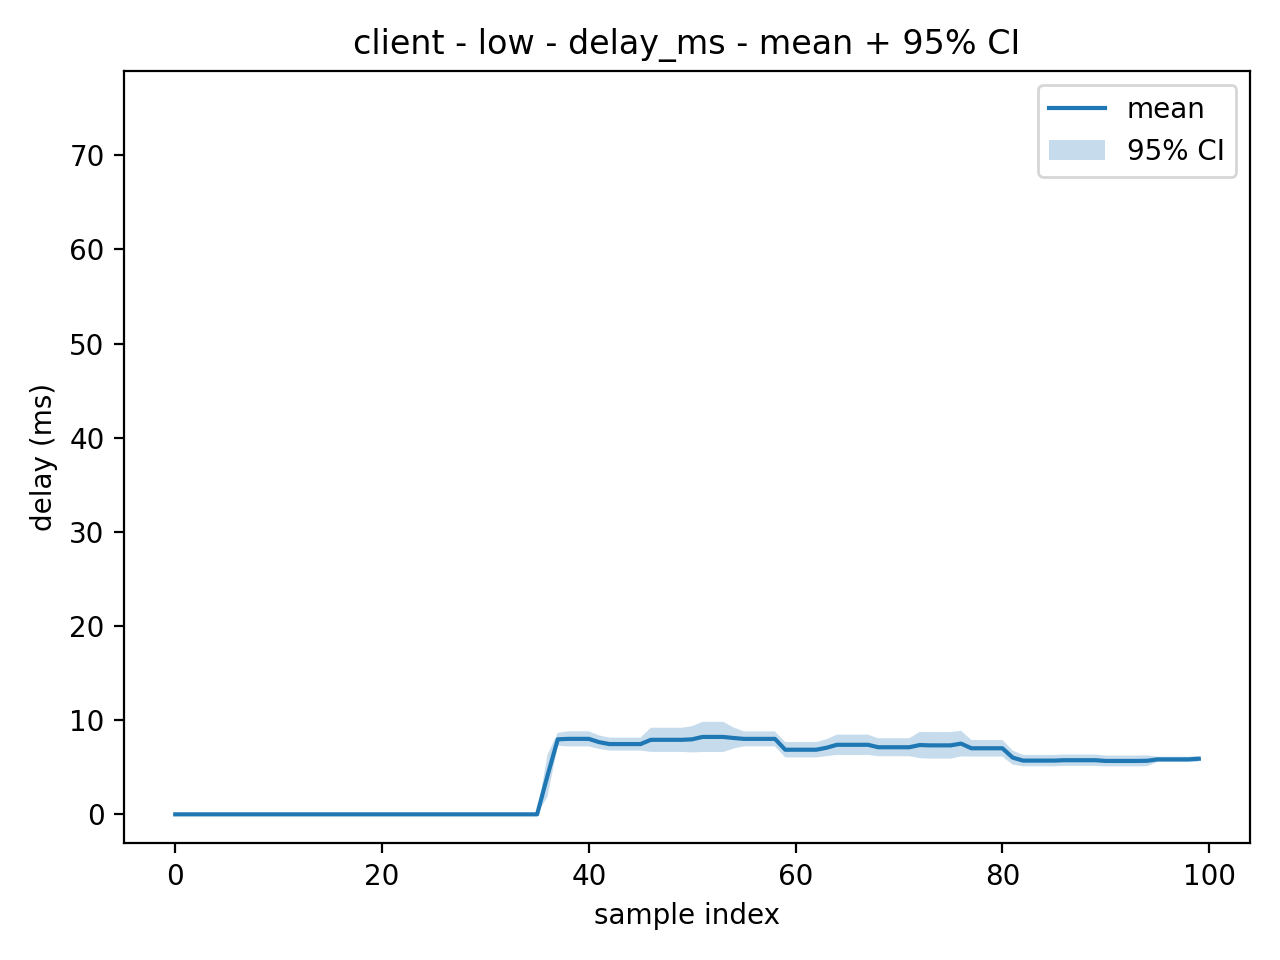
\includegraphics[width=\linewidth]{
      pars_plots/ntpsec/_aggregated/client/low/delay_ms_mean_ci95.png
    }
    \caption{Scenario LOW}
  \end{subfigure}
  \hfill
  \begin{subfigure}
    {0.32\textwidth}
    \centering
    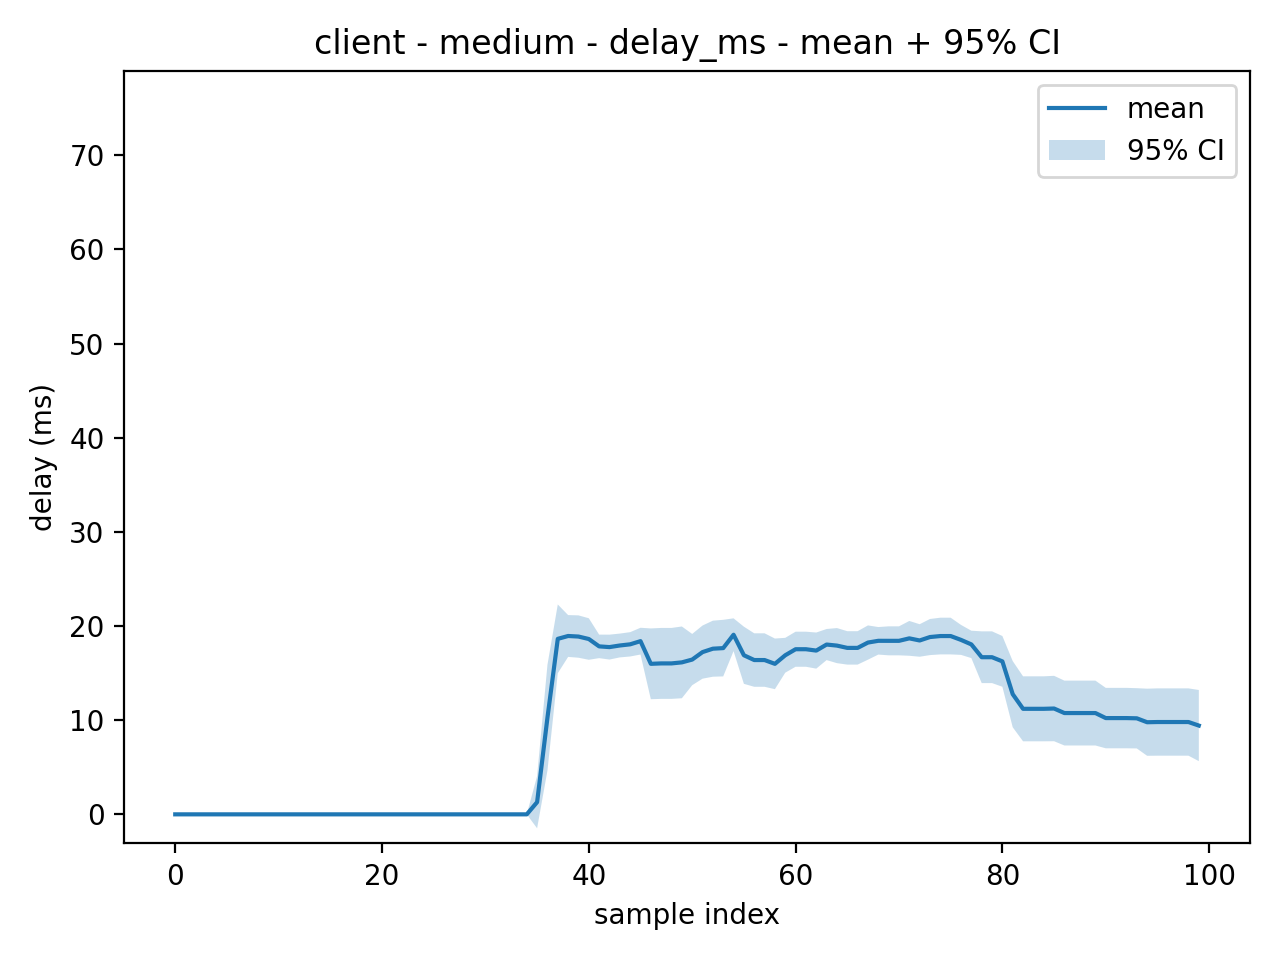
\includegraphics[width=\linewidth]{
      pars_plots/ntpsec/_aggregated/client/medium/delay_ms_mean_ci95.png
    }
    \caption{Scenario MEDIUM}
  \end{subfigure}
  \hfill
  \begin{subfigure}
    {0.32\textwidth}
    \centering
    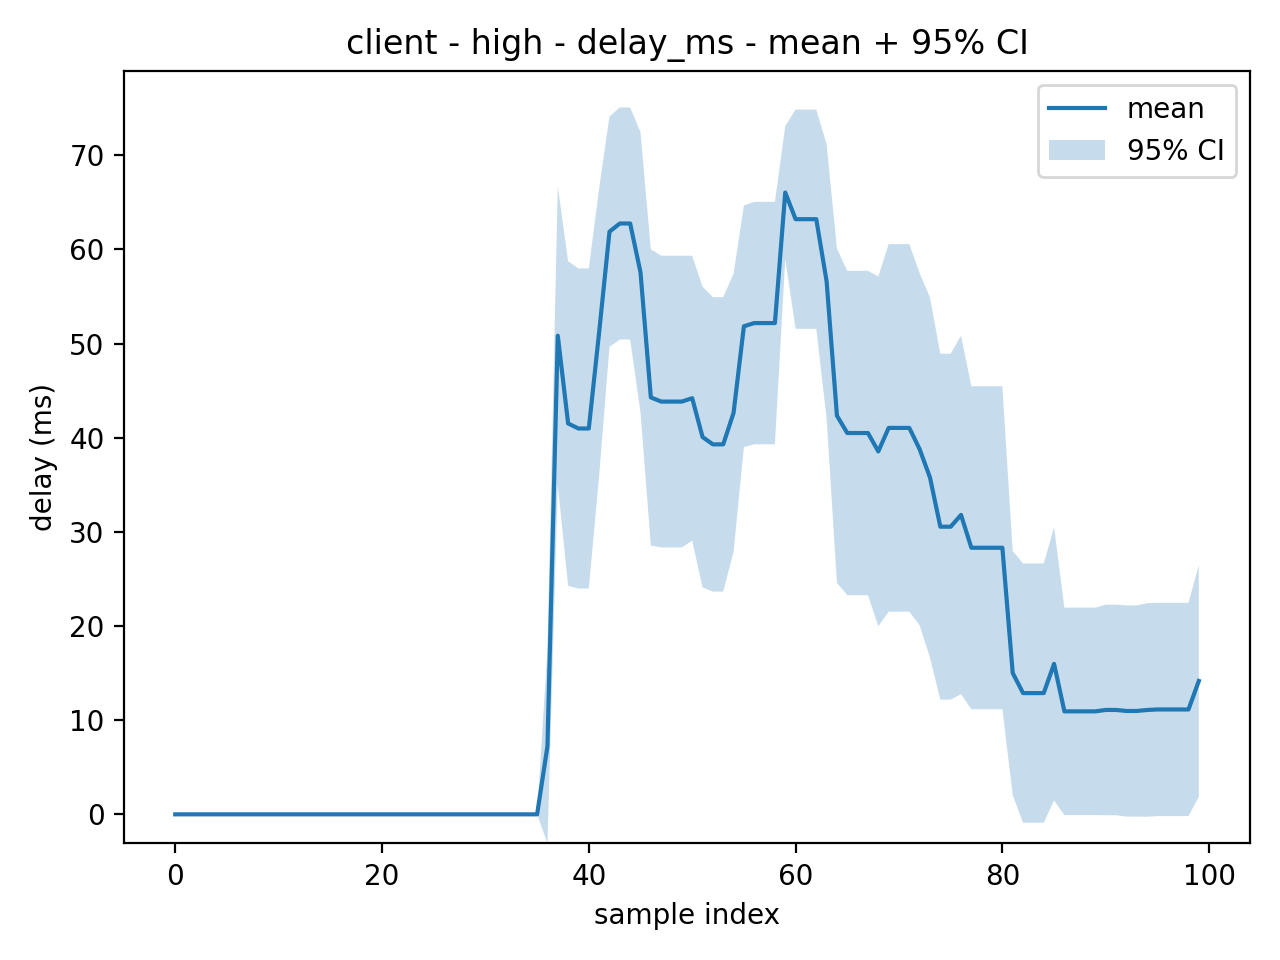
\includegraphics[width=\linewidth]{
      pars_plots/ntpsec/_aggregated/client/high/delay_ms_mean_ci95.png
    }
    \caption{Scenario HIGH}
  \end{subfigure}

  \caption{Media con intervallo di confidenza al 95\% - nodo: \texttt{clientntp}}
  \label{fig:scenario_comparison}
\end{figure}
\begin{figure}[H]
  \centering

  \begin{subfigure}
    {0.32\textwidth}
    \centering
    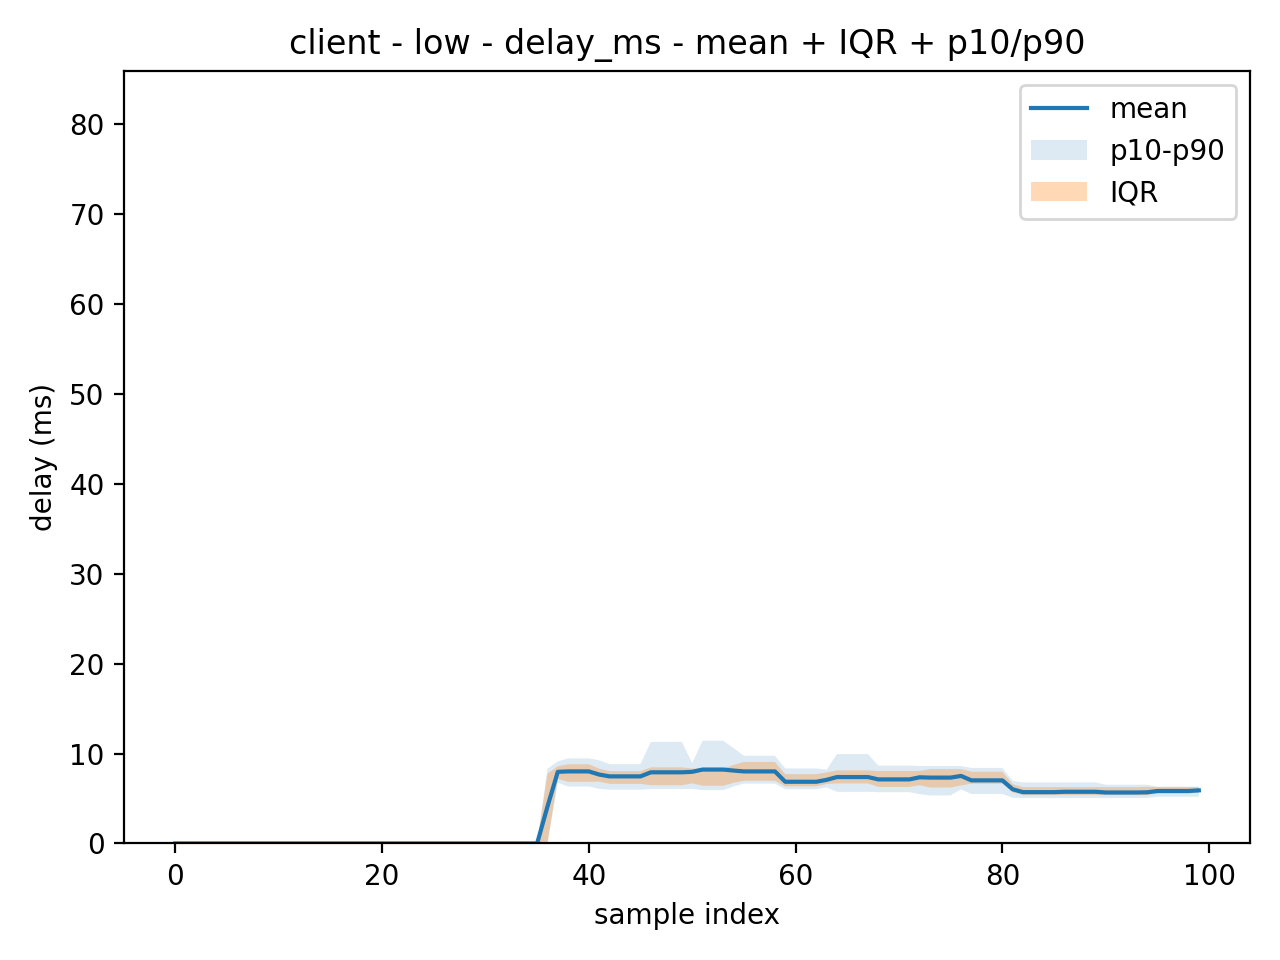
\includegraphics[width=\linewidth]{
      pars_plots/ntpsec/_aggregated/client/low/delay_ms_mean_iqr_p10_p90.png
    }
    \caption{Scenario LOW}
  \end{subfigure}
  \hfill
  \begin{subfigure}
    {0.32\textwidth}
    \centering
    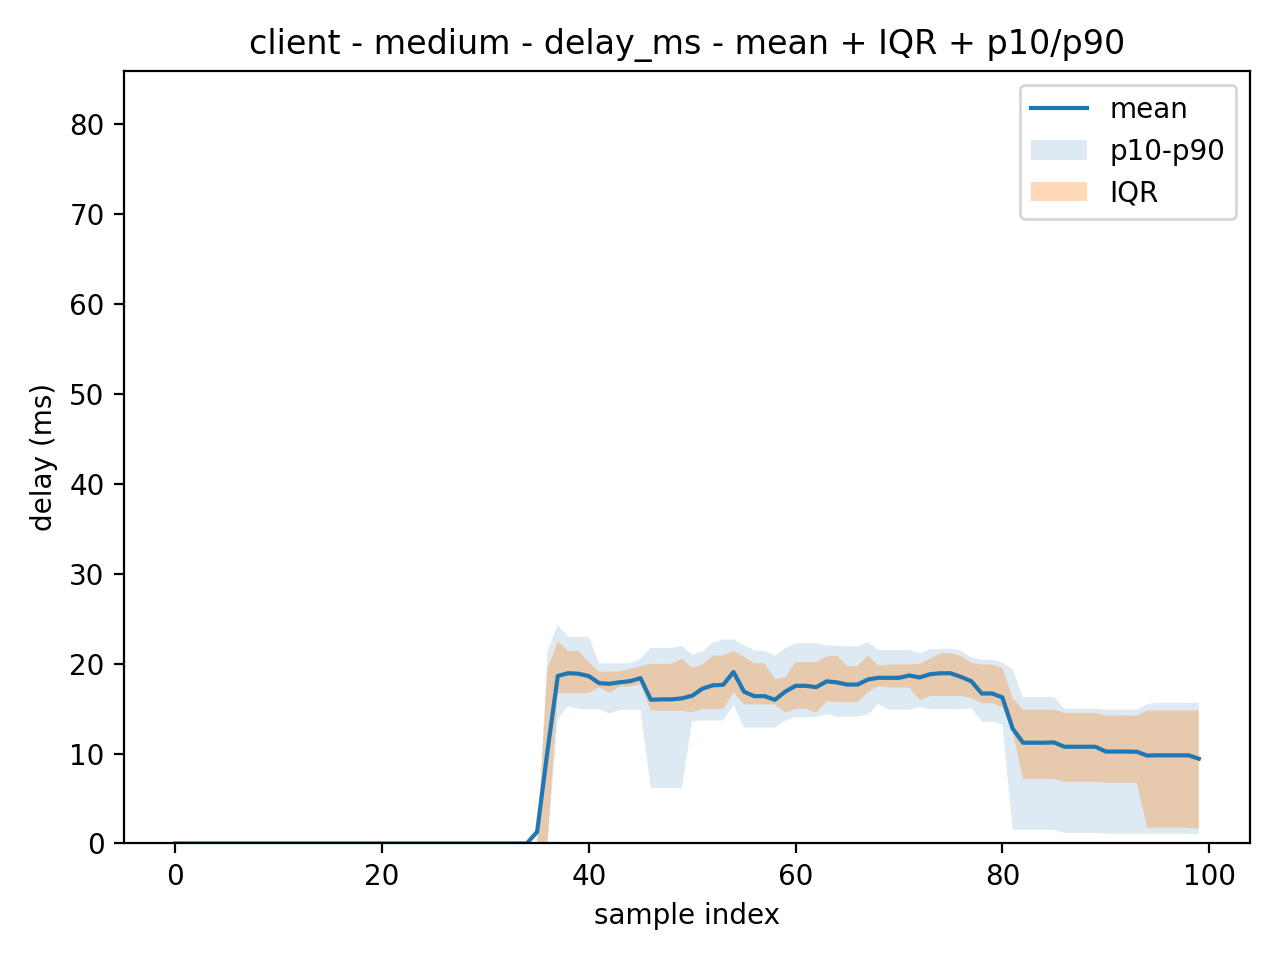
\includegraphics[width=\linewidth]{
      pars_plots/ntpsec/_aggregated/client/medium/delay_ms_mean_iqr_p10_p90.png
    }
    \caption{Scenario MEDIUM}
  \end{subfigure}
  \hfill
  \begin{subfigure}
    {0.32\textwidth}
    \centering
    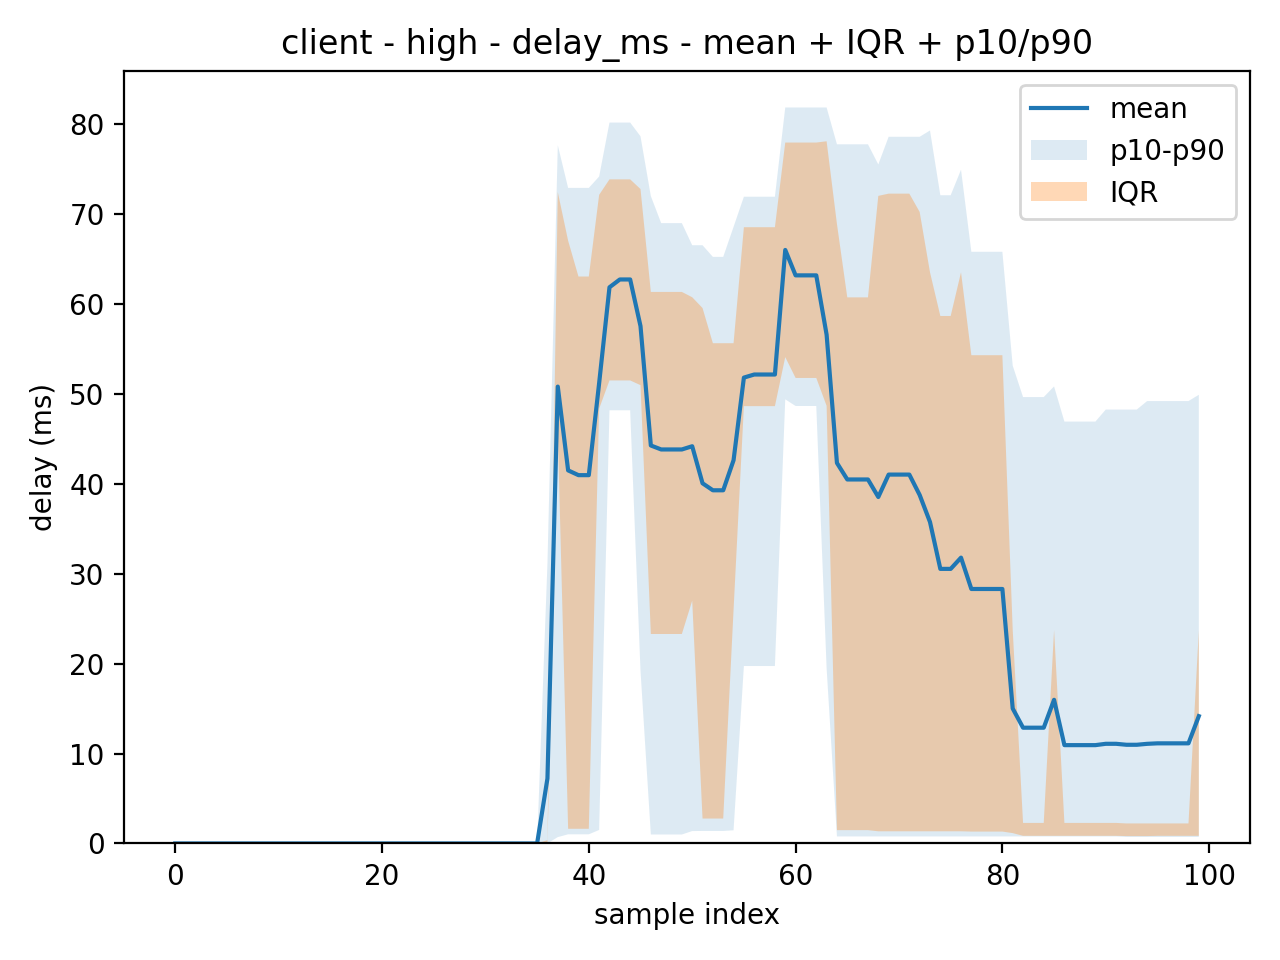
\includegraphics[width=\linewidth]{
      pars_plots/ntpsec/_aggregated/client/high/delay_ms_mean_iqr_p10_p90.png
    }
    \caption{Scenario HIGH}
  \end{subfigure}

  \caption{Media con banda interquartile e banda p10-p90 - nodo: \texttt{clientntp}}
  \label{fig:scenario_comparison}
\end{figure}
L’analisi del delay misurato sul nodo \texttt{clientntp} per il demone \texttt{NTPsec}
mostra una chiara dipendenza dalle condizioni di rete introdotte nei tre scenari sperimentali.
La metrica risulta particolarmente informativa perché riflette in modo diretto
il costo temporale del percorso di rete osservato dal demone durante il processo
di sincronizzazione. Per questa ragione, oltre al livello medio del delay, assumono
rilievo anche la sua stabilità nel tempo e l’ampiezza della variabilità tra le diverse
run.

Nello scenario \texttt{low}, il delay assume valori contenuti e presenta un andamento
complessivamente regolare. Dopo la fase iniziale, la curva media si colloca stabilmente
in una fascia di circa 6–8 ms, con oscillazioni moderate e bande di dispersione
relativamente strette. Considerando i soli campioni \texttt{post-selected}, il delay
medio è pari a circa 7.00 ms, con mediana 6.82 ms e intervallo interquartile
pari a circa 1.95 ms. Anche la dispersione lungo la curva aggregata rimane limitata:
la media della banda interquartile è di circa 1.43 ms, mentre la larghezza media della
banda p10–p90 è circa 2.85 ms. Nel complesso, il comportamento osservato è coerente
con uno scenario a basso impairment, nel quale il client raggiunge rapidamente
un regime relativamente stabile e mantiene una variabilità contenuta tra le run.

Nel caso \texttt{medium}, il delay cresce in modo netto e si colloca su una
fascia superiore rispetto al caso precedente. Dopo il primo aggancio, la curva
media si mantiene prevalentemente tra circa 16 e 19 ms per una parte consistente
dell’osservazione, per poi ridursi nella parte finale verso valori prossimi a 10 ms.
Sui campioni \texttt{post-selected}, il delay medio è circa 15.5 ms, con mediana 16.5
ms e intervallo interquartile di circa 5.18 ms. Rispetto allo scenario \texttt{low},
non aumenta soltanto il livello centrale della metrica, ma cresce anche la variabilità:
la larghezza media della banda IQR lungo la curva è circa 5.62 ms e quella
p10–p90 circa 10.0 ms. L’andamento resta leggibile e non presenta instabilità estreme,
ma mostra una sensibilità decisamente maggiore alle perturbazioni di rete. Il passaggio
da \texttt{low} a \texttt{medium} corrisponde quindi a un cambio di livello ben riconoscibile,
accompagnato da una dispersione più marcata.

Lo scenario \texttt{high} è quello che presenta il comportamento più degradato e meno
regolare. Dopo la selezione del peer, la curva media si colloca inizialmente su valori
molto elevati, spesso compresi tra circa 40 e 65 ms, con oscillazioni ampie e una
forte eterogeneità tra run, come evidenziato dall’allargamento delle bande di
dispersione. Nella parte finale della serie si osserva una riduzione del livello medio
verso valori attorno a 10–15 ms, ma tale riduzione non elimina la marcata
instabilità osservata nella parte centrale del tracciato. Sui campioni \texttt{post-selected},
il delay medio è pari a circa 35.0 ms, con mediana 46.7 ms e intervallo
interquartile molto ampio, pari a circa 59.9 ms. Anche le statistiche della
curva aggregata confermano questa forte dispersione: la larghezza media della banda
IQR è circa 31.0 ms e quella p10–p90 circa 59.4 ms. Ne risulta uno scenario in
cui il degrado di rete non produce soltanto un incremento del ritardo osservato, ma
anche una forte perdita di stabilità e di omogeneità tra le differenti run.

Il confronto tra i tre scenari mostra quindi una progressione complessivamente coerente
con l’aumento della severità degli impairment di rete. Passando da \texttt{low} a
\texttt{medium}, il delay del client cresce in modo evidente e la dispersione aumenta
sensibilmente, pur mantenendo una dinamica ancora relativamente controllata. Il passaggio
a \texttt{high} introduce invece una discontinuità più marcata: il livello medio si
sposta su valori molto superiori e la variabilità si amplia in modo sostanziale,
segnalando una condizione di sincronizzazione molto meno stabile. In termini qualitativi,
la metrica del delay risulta quindi efficace nel discriminare i tre scenari e
nel mostrare come l’incremento del degrado di rete si traduca, per il nodo client
NTPsec, in un peggioramento sia del livello della misura sia della sua
regolarità temporale.
\subsubsection{Analisi metrica: \texttt{jitter}}
\begin{figure}[H]
  \centering

  \begin{subfigure}
    {0.32\textwidth}
    \centering
    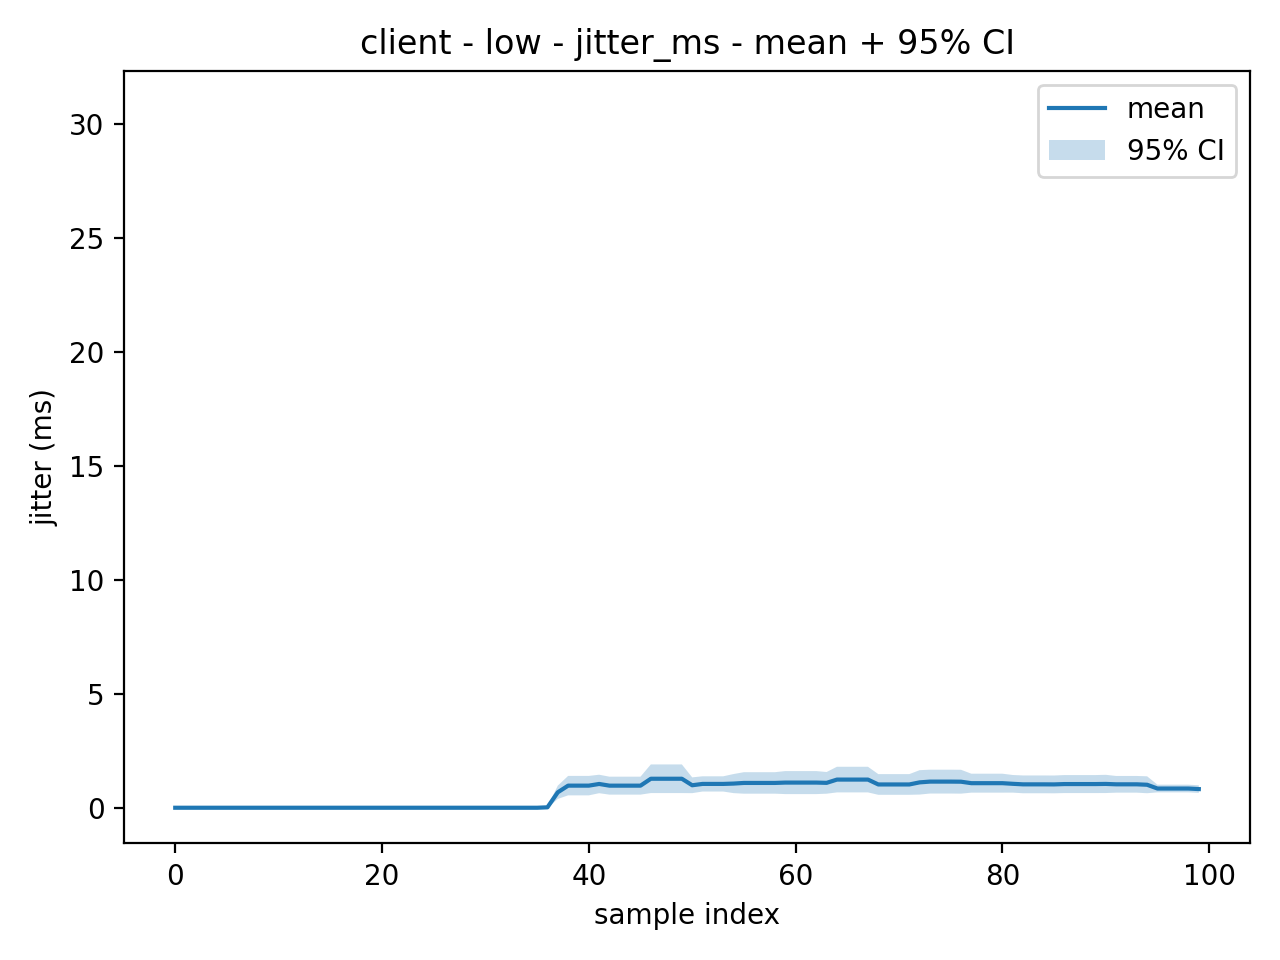
\includegraphics[width=\linewidth]{
      pars_plots/ntpsec/_aggregated/client/low/jitter_ms_mean_ci95.png
    }
    \caption{Scenario LOW}
  \end{subfigure}
  \hfill
  \begin{subfigure}
    {0.32\textwidth}
    \centering
    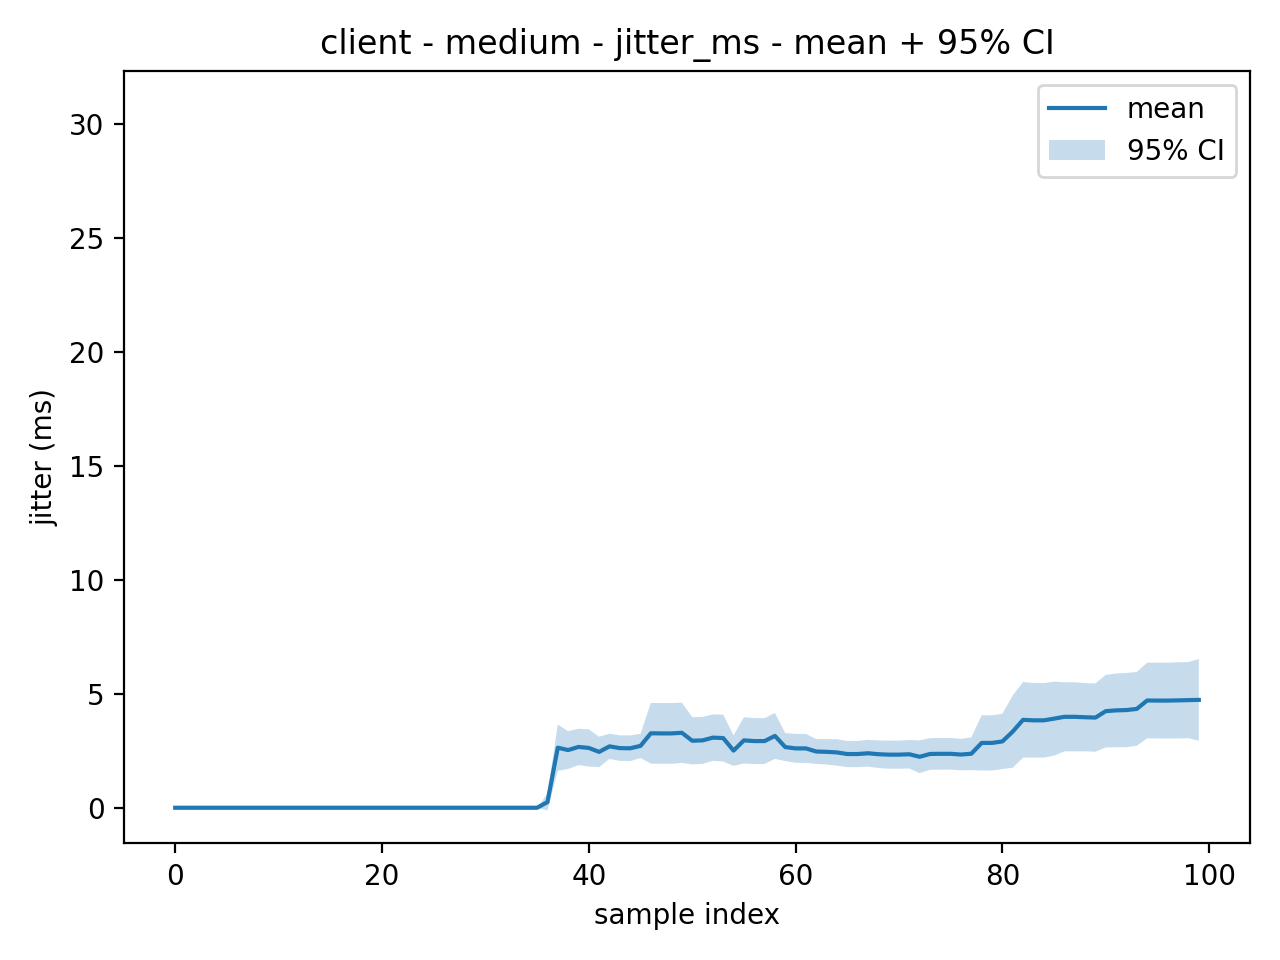
\includegraphics[width=\linewidth]{
      pars_plots/ntpsec/_aggregated/client/medium/jitter_ms_mean_ci95.png
    }
    \caption{Scenario MEDIUM}
  \end{subfigure}
  \hfill
  \begin{subfigure}
    {0.32\textwidth}
    \centering
    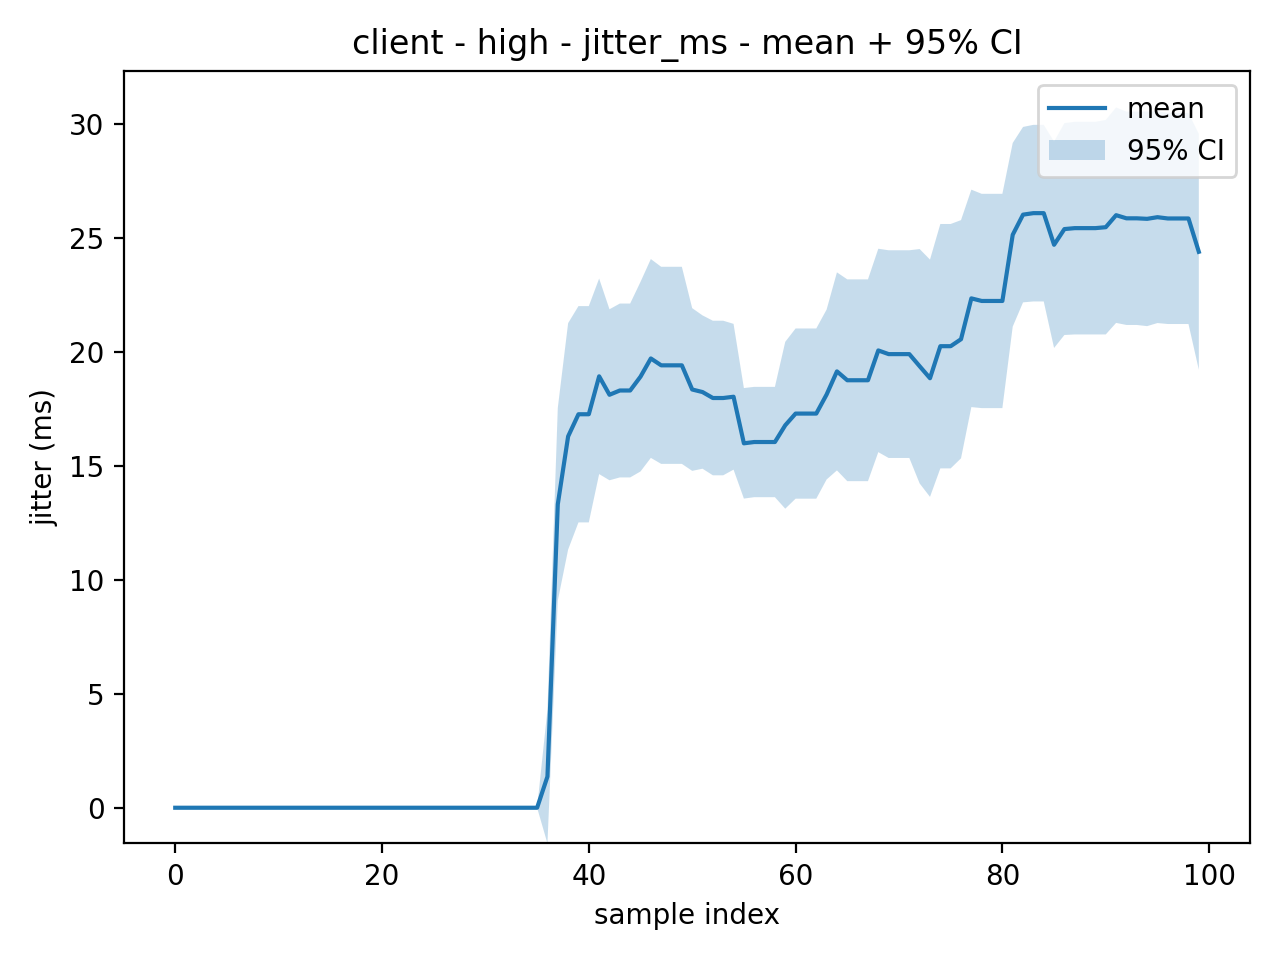
\includegraphics[width=\linewidth]{
      pars_plots/ntpsec/_aggregated/client/high/jitter_ms_mean_ci95.png
    }
    \caption{Scenario HIGH}
  \end{subfigure}

  \caption{Media con intervallo di confidenza al 95\% - nodo: \texttt{clientntp}}
  \label{fig:scenario_comparison}
\end{figure}
\begin{figure}[H]
  \centering

  \begin{subfigure}
    {0.32\textwidth}
    \centering
    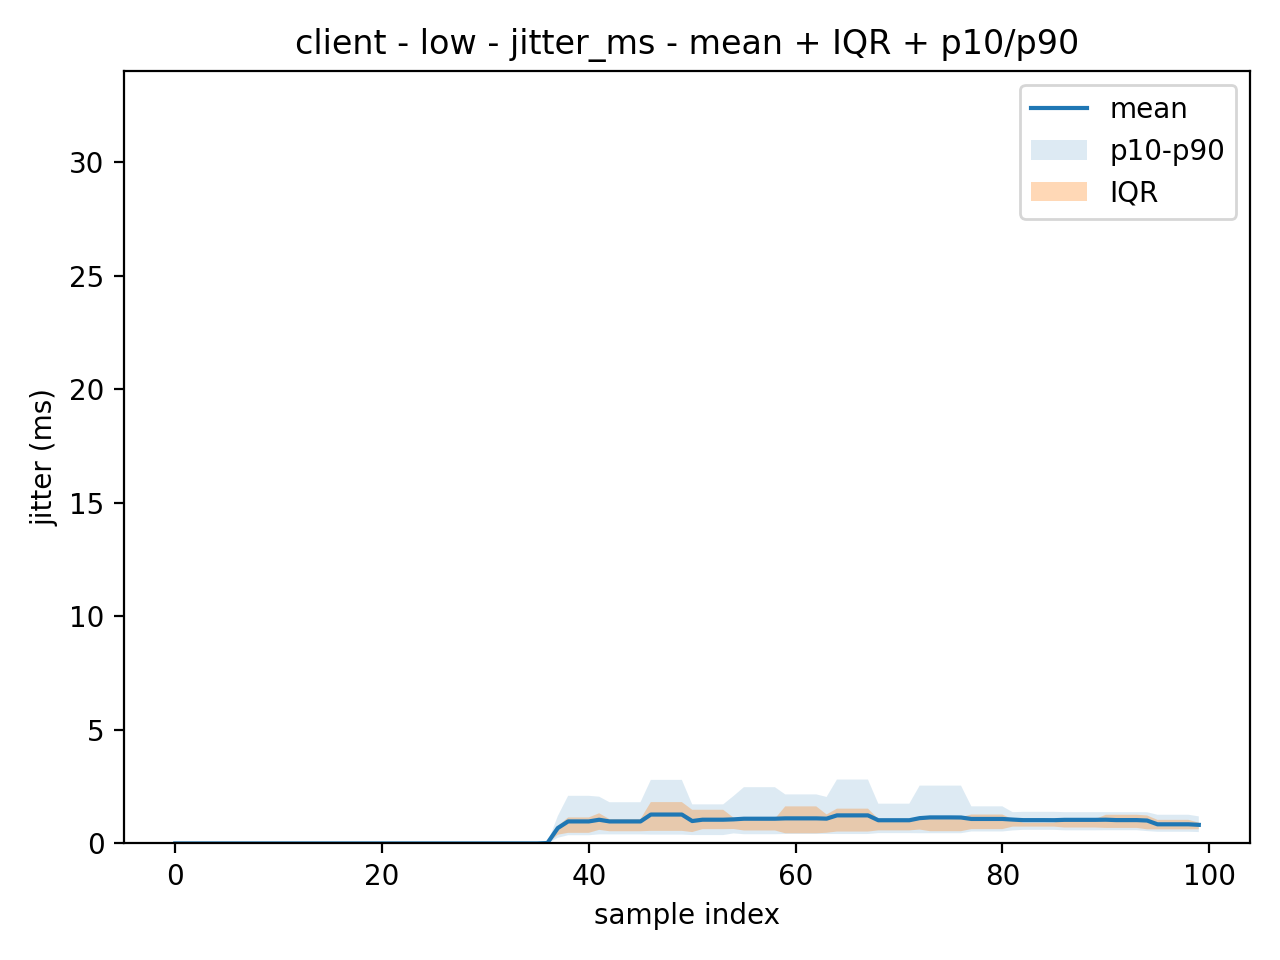
\includegraphics[width=\linewidth]{
      pars_plots/ntpsec/_aggregated/client/low/jitter_ms_mean_iqr_p10_p90.png
    }
    \caption{Scenario LOW}
  \end{subfigure}
  \hfill
  \begin{subfigure}
    {0.32\textwidth}
    \centering
    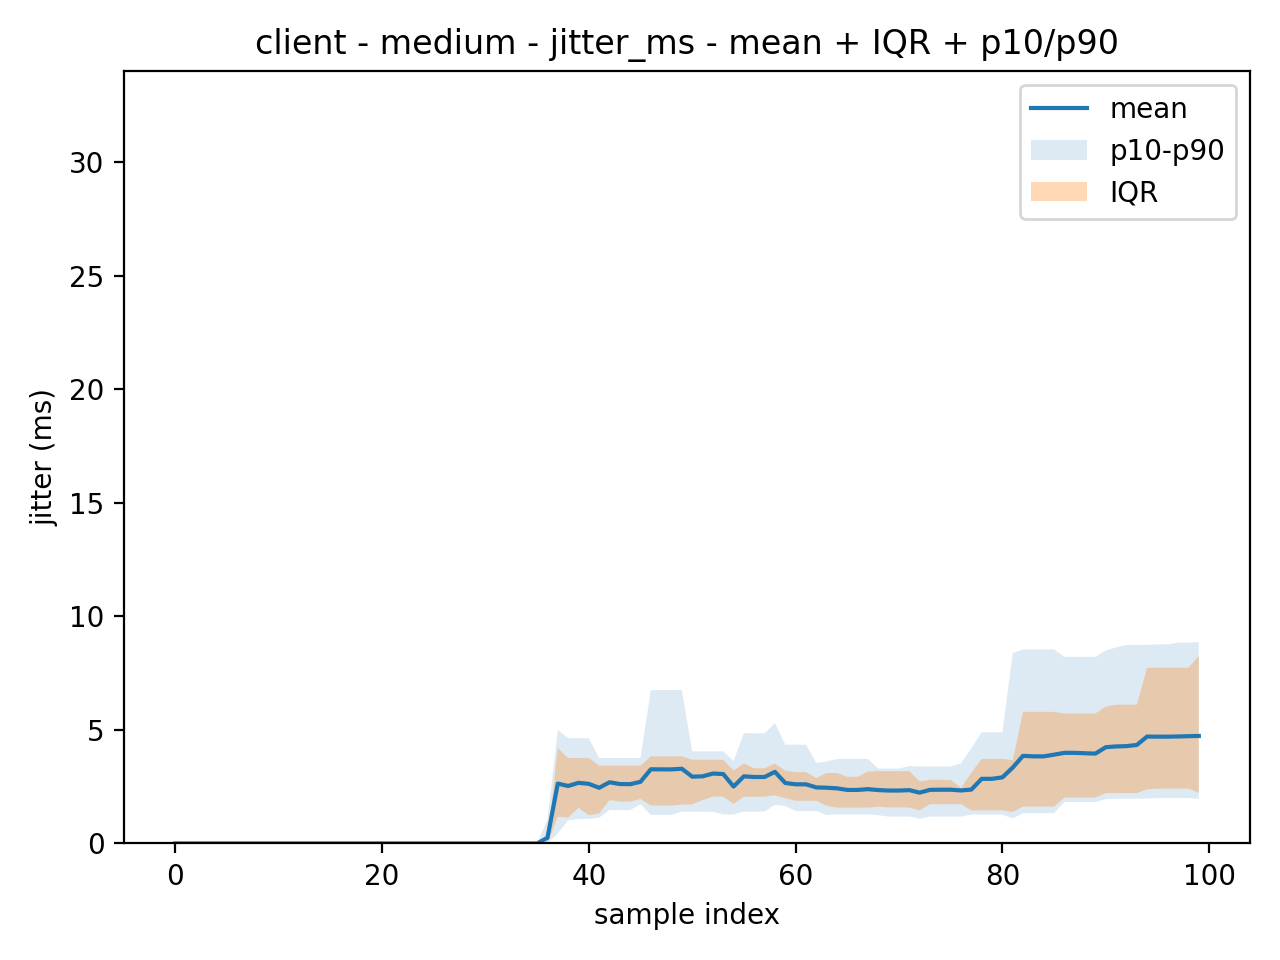
\includegraphics[width=\linewidth]{
      pars_plots/ntpsec/_aggregated/client/medium/jitter_ms_mean_iqr_p10_p90.png
    }
    \caption{Scenario MEDIUM}
  \end{subfigure}
  \hfill
  \begin{subfigure}
    {0.32\textwidth}
    \centering
    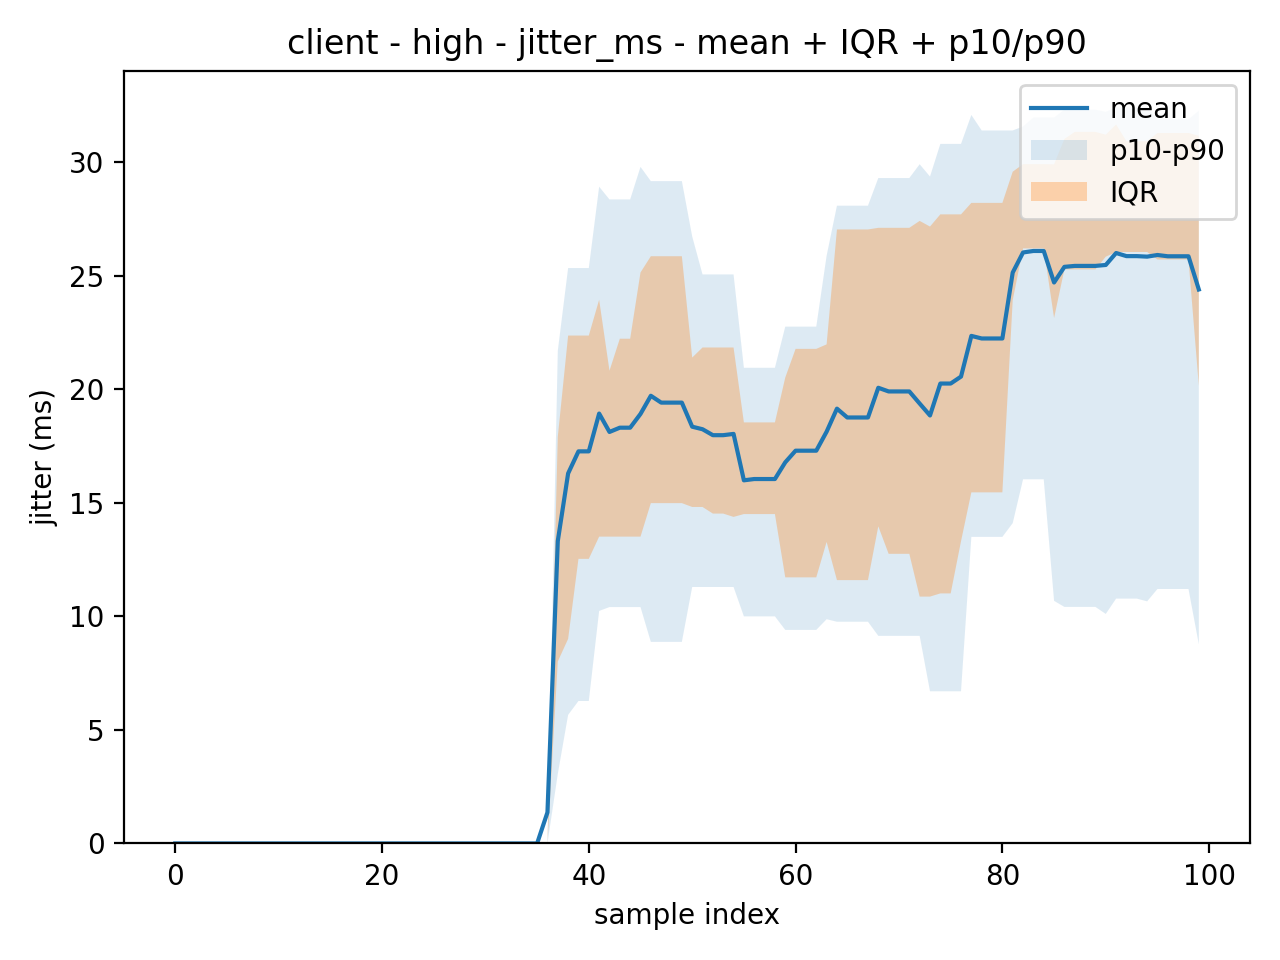
\includegraphics[width=\linewidth]{
      pars_plots/ntpsec/_aggregated/client/high/jitter_ms_mean_iqr_p10_p90.png
    }
    \caption{Scenario HIGH}
  \end{subfigure}

  \caption{Media con banda interquartile e banda p10-p90 - nodo: \texttt{clientntp}}
  \label{fig:scenario_comparison}
\end{figure}

L’analisi del jitter misurato sul nodo client per il demone NTPsec evidenzia una
chiara dipendenza dal livello di impairment introdotto nei tre scenari
sperimentali. La metrica mostra infatti un incremento progressivo sia del livello
medio sia della variabilità all’aumentare della severità delle condizioni di rete.

Nello scenario \texttt{low}, una volta superata la fase iniziale precedente alla selezione
del peer di sincronizzazione, il jitter si mantiene su valori contenuti e
relativamente regolari. Considerando i soli campioni \texttt{post-selected}, il valore
medio risulta pari a circa 1.05 ms, con una dispersione moderata: la banda interquartile
media della curva aggregata è pari a circa 0.65 ms, mentre la banda p10--p90 si attesta
intorno a 1.46 ms. Il comportamento osservato è quindi compatibile con una
condizione di rete stabile, nella quale il client mantiene una sincronizzazione sufficientemente
regolare.

Nel caso \texttt{medium}, il jitter cresce in modo evidente e si colloca su una fascia
sensibilmente superiore. Sui campioni post-selected il valore medio è pari a
circa 3.14 ms, cioè circa tre volte il corrispondente valore osservato nello scenario
\texttt{low}. Parallelamente aumenta anche la dispersione, con una banda
interquartile media di circa 2.40 ms e una banda p10--p90 di circa 4.18 ms. Il
sistema resta complessivamente stabile, ma il processo di sincronizzazione risulta
più sensibile alla variabilità introdotta dalla rete.

Lo scenario \texttt{high} presenta il comportamento più degradato. Dopo la fase iniziale,
il jitter assume valori elevati lungo l’intera serie aggregata, con media post-selected
pari a circa 20.9 ms. L’incremento rispetto allo scenario \texttt{medium} è molto
marcato, e rispetto allo scenario \texttt{low} il divario diventa di un ordine di
grandezza. Anche la dispersione aumenta nettamente: la banda interquartile media raggiunge
circa 9.38 ms, mentre la banda p10--p90 arriva a circa 18.3 ms. Il grafico
evidenzia inoltre oscillazioni ampie e persistenti, indicative di una condizione di
sincronizzazione significativamente meno regolare.

Nel complesso, la metrica del jitter sul client NTPsec mostra una progressione
coerente con l’aumento della severità degli impairment di rete. Il passaggio da \texttt{low}
a \texttt{medium} comporta già un deterioramento misurabile, mentre il passaggio
a \texttt{high} introduce un cambiamento di regime molto più netto,
caratterizzato da valori medi elevati e da una dispersione significativamente
maggiore. La metrica risulta pertanto efficace nel mettere in evidenza l’impatto del
degrado di rete sulla stabilità temporale del client.

\subsubsection{Analisi metrica: \texttt{offset}}
\begin{figure}[H]
  \centering

  \begin{subfigure}
    {0.32\textwidth}
    \centering
    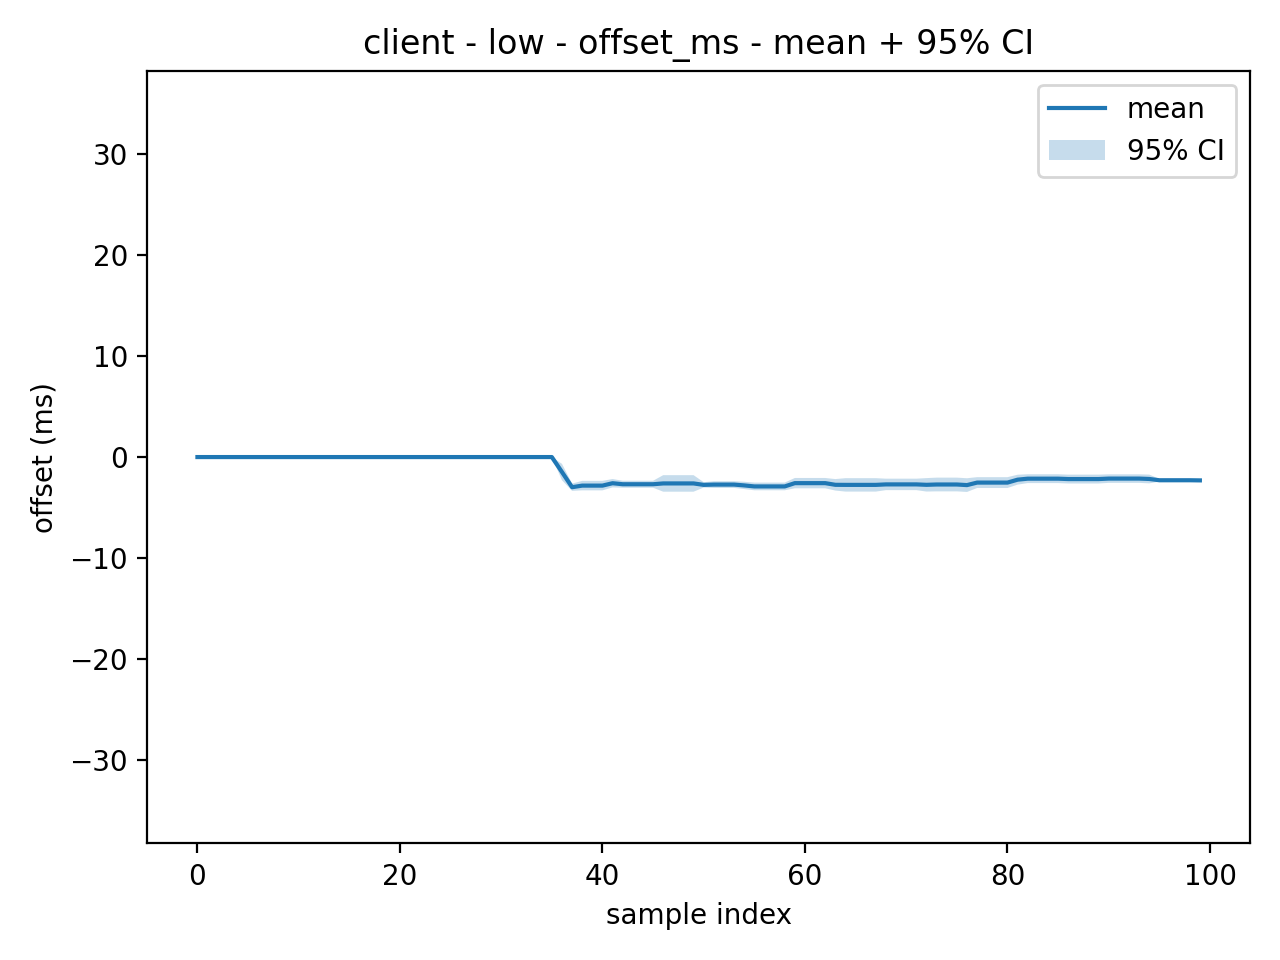
\includegraphics[width=\linewidth]{
      pars_plots/ntpsec/_aggregated/client/low/offset_ms_mean_ci95.png
    }
    \caption{Scenario LOW}
  \end{subfigure}
  \hfill
  \begin{subfigure}
    {0.32\textwidth}
    \centering
    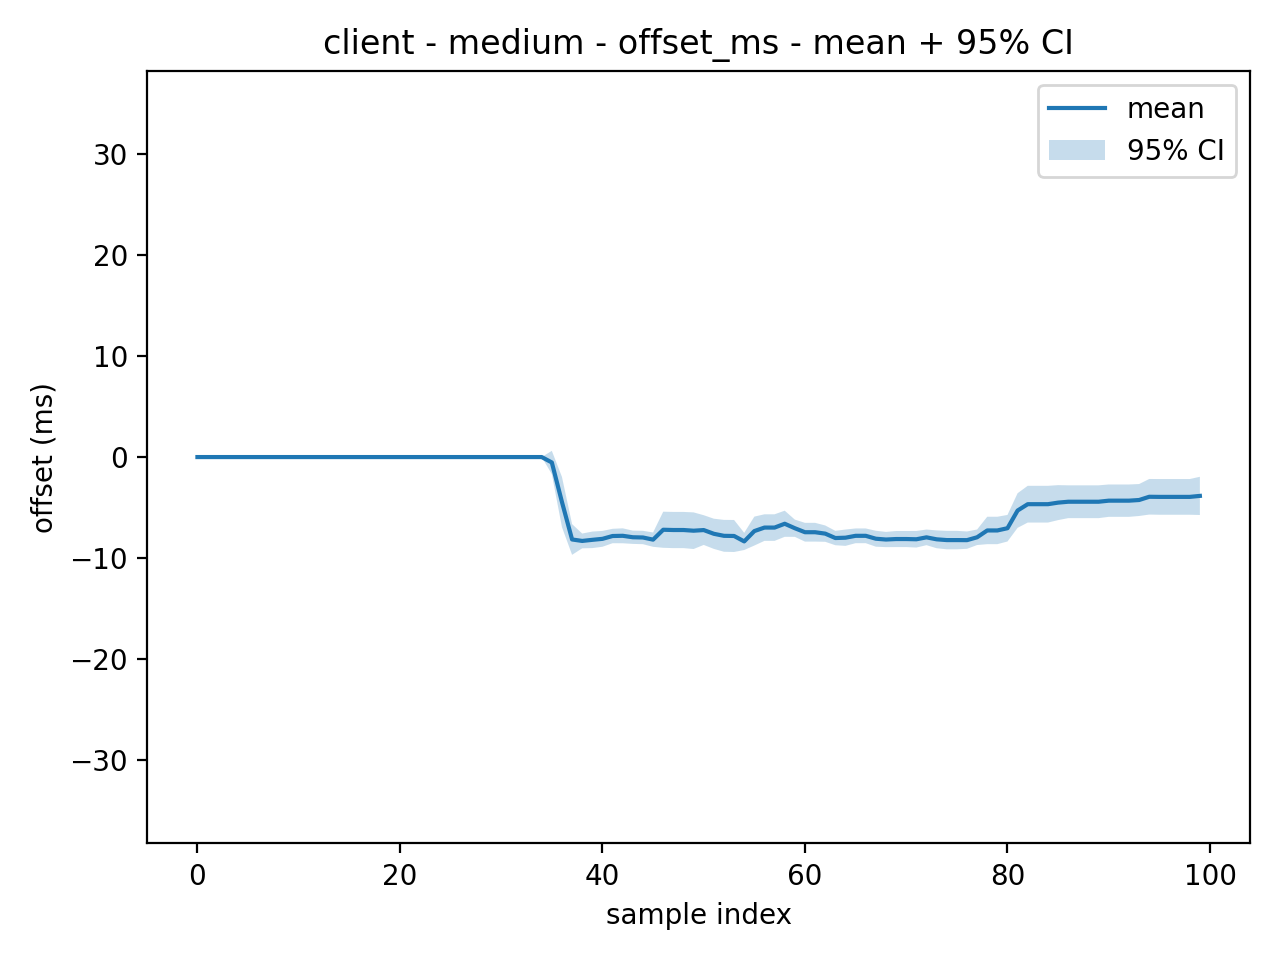
\includegraphics[width=\linewidth]{
      pars_plots/ntpsec/_aggregated/client/medium/offset_ms_mean_ci95.png
    }
    \caption{Scenario MEDIUM}
  \end{subfigure}
  \hfill
  \begin{subfigure}
    {0.32\textwidth}
    \centering
    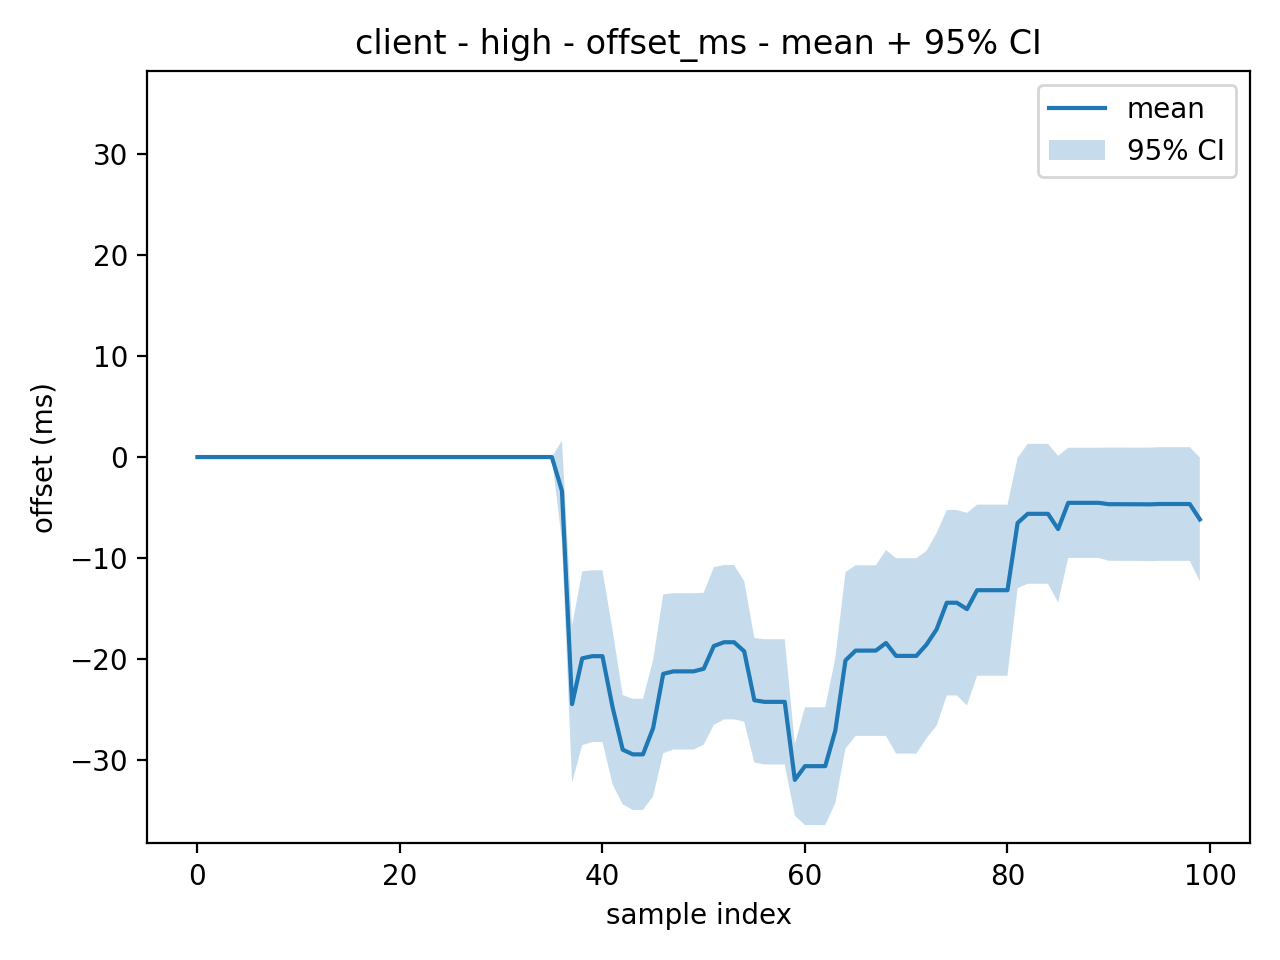
\includegraphics[width=\linewidth]{
      pars_plots/ntpsec/_aggregated/client/high/offset_ms_mean_ci95.png
    }
    \caption{Scenario HIGH}
  \end{subfigure}

  \caption{Media con intervallo di confidenza al 95\% - nodo: \texttt{clientntp}}
  \label{fig:scenario_comparison}
\end{figure}
\begin{figure}[H]
  \centering

  \begin{subfigure}
    {0.32\textwidth}
    \centering
    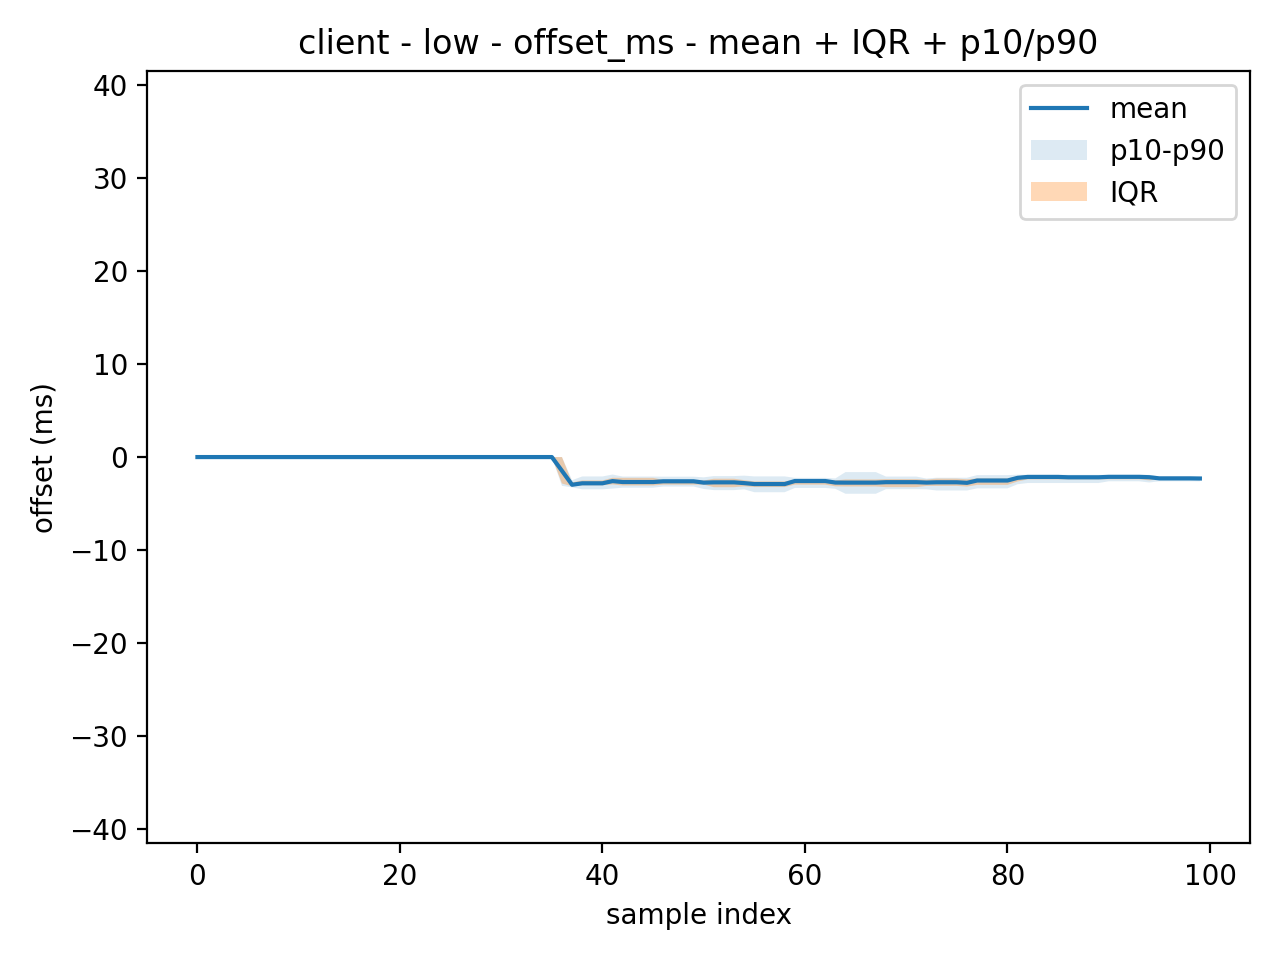
\includegraphics[width=\linewidth]{
      pars_plots/ntpsec/_aggregated/client/low/offset_ms_mean_iqr_p10_p90.png
    }
    \caption{Scenario LOW}
  \end{subfigure}
  \hfill
  \begin{subfigure}
    {0.32\textwidth}
    \centering
    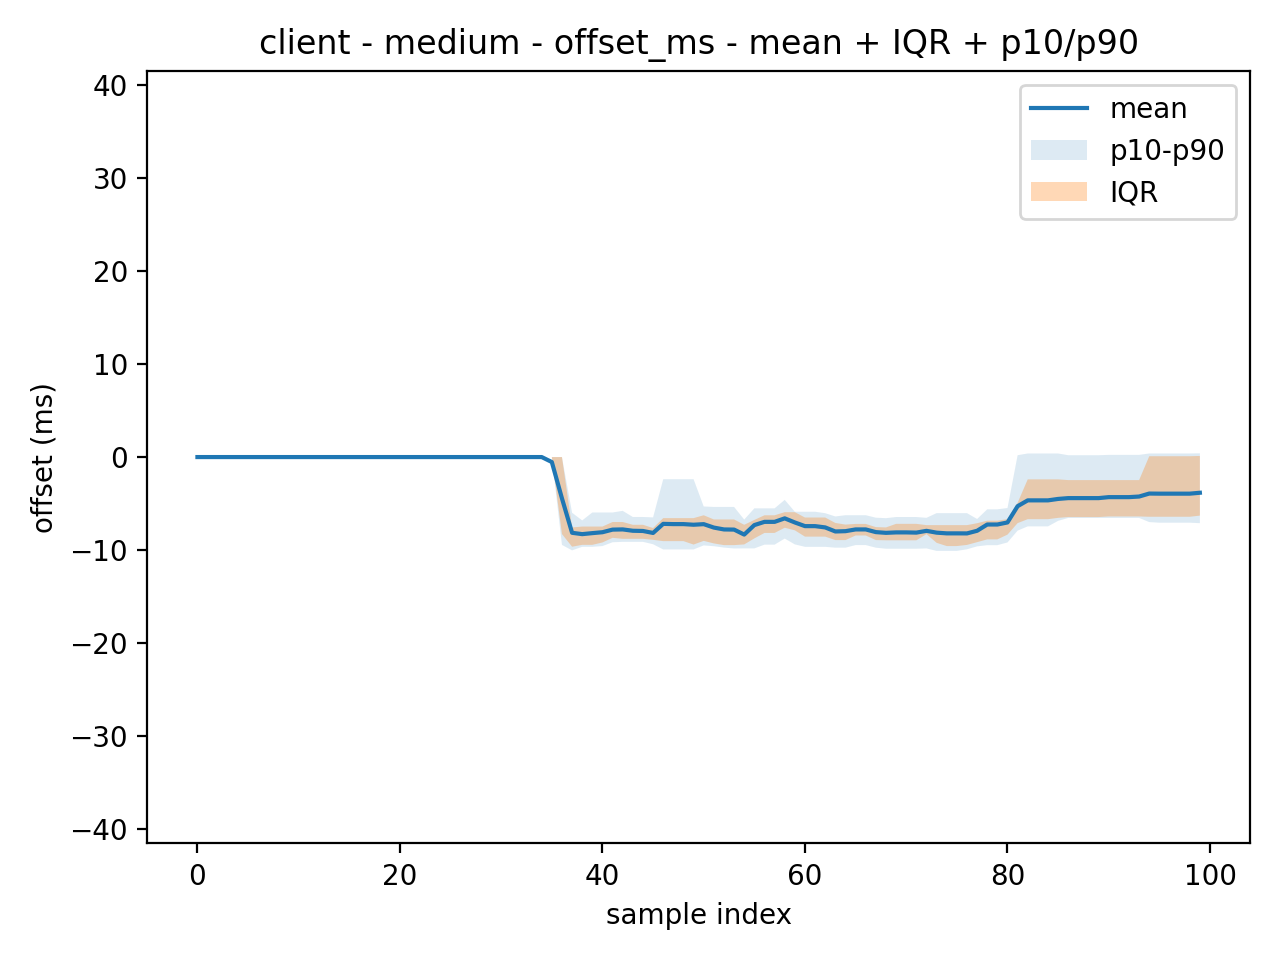
\includegraphics[width=\linewidth]{
      pars_plots/ntpsec/_aggregated/client/medium/offset_ms_mean_iqr_p10_p90.png
    }
    \caption{Scenario MEDIUM}
  \end{subfigure}
  \hfill
  \begin{subfigure}
    {0.32\textwidth}
    \centering
    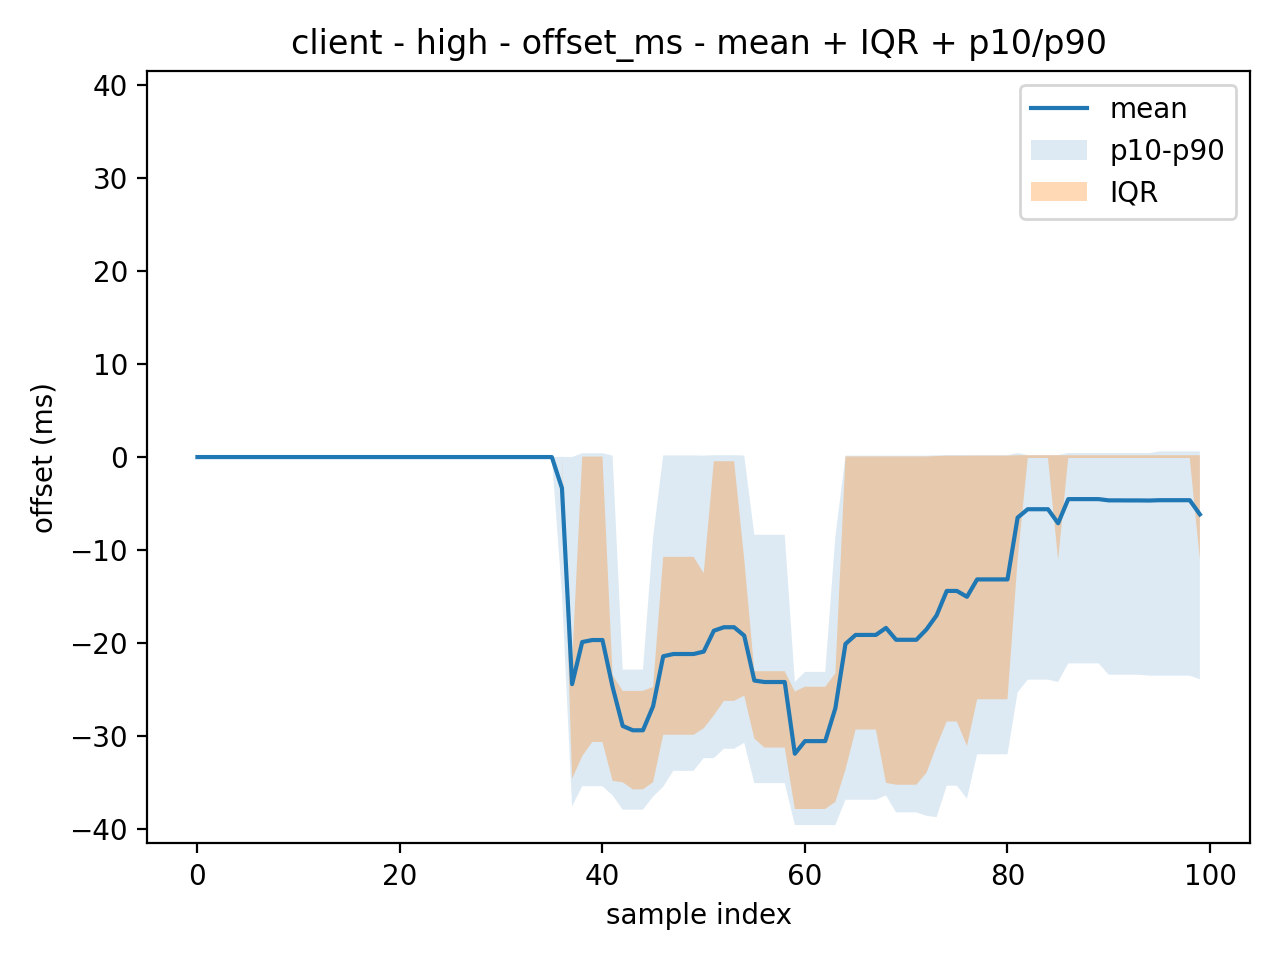
\includegraphics[width=\linewidth]{
      pars_plots/ntpsec/_aggregated/client/high/offset_ms_mean_iqr_p10_p90.png
    }
    \caption{Scenario HIGH}
  \end{subfigure}

  \caption{Media con banda interquartile e banda p10-p90 - nodo: \texttt{clientntp}}
  \label{fig:scenario_comparison}
\end{figure}

L’analisi dell’offset misurato sul nodo client per il demone \texttt{NTPsec} evidenzia
una chiara dipendenza dal livello di impairment introdotto nei tre scenari sperimentali.
La metrica assume valori sistematicamente negativi dopo la selezione del peer di
riferimento, indicando quindi una deviazione del clock locale rispetto al riferimento
temporale nella medesima direzione lungo tutto l’intervallo di osservazione utile.
Il confronto tra gli scenari mostra che, al crescere della severità delle condizioni
di rete, aumenta sia il modulo dell’offset sia la sua variabilità tra le diverse
run.

Nello scenario \texttt{low}, dopo la fase iniziale in cui la misura rimane nulla
prima della selezione effettiva del peer, l’offset si stabilizza rapidamente su valori
contenuti e relativamente regolari, collocandosi attorno a $-2.5$/$-3\,\mathrm{ms}$.
Considerando i soli campioni successivi alla selezione, si osserva una media
pari a circa $-2.55\,\mathrm{ms}$ e una mediana pressoché coincidente, pari a $-2
.55\,\mathrm{ms}$, con una dispersione moderata ($\sigma \approx 0.91\,\mathrm{ms}$).
Anche la curva aggregata conferma tale stabilità: il valore medio centrale
risulta pari a circa $-2.55\,\mathrm{ms}$, mentre l’ampiezza media della banda interquartile
resta contenuta ($\mathrm{IQR}\approx 0.56\,\mathrm{ms}$), così come la fascia
$p10$--$p90$ ($\approx 1.21\,\mathrm{ms}$). Nel complesso, il comportamento osservato
nello scenario \texttt{low} appare quindi stabile e caratterizzato da uno
scostamento limitato rispetto al riferimento.

Nel caso \texttt{medium}, la curva dell’offset si sposta in modo netto verso
valori più negativi. Dopo la transizione iniziale, la misura si colloca per gran
parte dell’intervallo osservato in una fascia prossima a $-7$/$-8\,\mathrm{ms}$, con
una lieve risalita nella parte finale della serie. Sui campioni post-selezione
la media è pari a circa $-6.70\,\mathrm{ms}$, con mediana pari a $-7.08\,\mathrm{ms}$
e deviazione standard di circa $2.81\,\mathrm{ms}$. Anche in questo caso la
curva aggregata restituisce un quadro coerente: il valor medio centrale è pari a circa
$-6.69\,\mathrm{ms}$, mentre la variabilità cresce rispetto allo scenario
precedente, come mostrato dall’aumento dell’ampiezza media della banda interquartile
($\approx 2.74\,\mathrm{ms}$) e della fascia $p10$--$p90$ ($\approx 4.97\,\mathrm{ms}$).
Rispetto allo scenario \texttt{low} si osserva quindi non solo un incremento del
modulo dell’offset, ma anche una minore regolarità della misura nel corso delle run.

Lo scenario \texttt{high} presenta il comportamento più degradato tra i tre
considerati. Dopo la fase iniziale, l’offset assume valori fortemente negativi, con
escursioni ampie e un andamento sensibilmente meno regolare rispetto ai casi precedenti.
La curva aggregata mostra infatti una permanenza prolungata in una fascia
compresa approssimativamente tra $-20$ e $-30\,\mathrm{ms}$, seguita da una successiva
risalita verso valori meno negativi nella parte finale della sequenza. Le
statistiche post-selezione confermano questo quadro: la media risulta pari a circa
$-16.42\,\mathrm{ms}$, la mediana a $-21.87\,\mathrm{ms}$ e la deviazione
standard a circa $15.38\,\mathrm{ms}$. Anche gli indicatori derivati dalla curva aggregata
mostrano una dispersione nettamente superiore rispetto agli altri scenari:
l’ampiezza media della banda interquartile è pari a circa $15.17\,\mathrm{ms}$, mentre
la fascia $p10$--$p90$ raggiunge in media circa $29.44\,\mathrm{ms}$. Il minimo della
curva media aggregata scende inoltre fino a circa $-30.12\,\mathrm{ms}$,
indicando la presenza di run con scostamenti temporali decisamente più marcati.

Nel complesso, il confronto tra i tre scenari mostra una progressione coerente del
degrado della metrica al crescere della severità degli impairment di rete. Il
passaggio da \texttt{low} a \texttt{medium} comporta un incremento netto del
modulo dell’offset e della dispersione associata; il passaggio da \texttt{medium}
a \texttt{high} introduce un ulteriore peggioramento, molto più marcato, caratterizzato
da valori medi più distanti dallo zero e da una variabilità significativamente maggiore
tra le run. Per questa metrica, l’uso dei campioni successivi alla selezione del peer
risulta particolarmente utile, poiché consente di isolare la fase effettiva di
sincronizzazione ed evitare che la presenza dei campioni iniziali nulli attenui
artificialmente il livello medio dello scostamento osservato.

\subsection{\texttt{boundary}}
Nel caso del nodo \texttt{boundary}, l’interpretazione dei risultati richiede
una precisazione preliminare. A differenza di quanto osservato sul nodo \texttt{clientntp},
gli impairment di rete introdotti mediante \texttt{tc/netem} non agiscono
direttamente sul collegamento \texttt{upstream} tra il nodo \texttt{boundary} e
il nodo di riferimento, bensì sul ramo \texttt{downstream} tra \texttt{boundary} e
\texttt{clientntp}. Ne consegue che le metriche rilevate sul \texttt{boundary}
non dovrebbero, in linea teorica, risentire in modo marcato del degrado
introdotto nei tre scenari sperimentali, o comunque non con la stessa intensità osservata
nel caso del clientntp.

L’analisi delle metriche del nodo \texttt{boundary} è pertanto orientata
principalmente a verificare la coerenza tra tale aspettativa teorica e i dati
effettivamente osservati. In particolare, il confronto tra scenari è finalizzato
a stabilire se le eventuali differenze rilevate siano effettivamente contenute, come
atteso, oppure se emergano variazioni non trascurabili che possano suggerire
effetti indiretti del degrado di rete sul comportamento del nodo.

Va inoltre considerato che il tempo di ingresso nel regime operativo può
differire rispetto a quello osservato sul nodo \texttt{clientntp}. Tale aspetto
viene tenuto in considerazione nell’interpretazione dei risultati, pur non costituendo,
di per sé, l’oggetto principale del confronto tra scenari.

\subsubsection{Analisi metriche: \texttt{delay, jitter, offset}}
\begin{figure}[H]
  \centering

  \begin{subfigure}
    {0.32\textwidth}
    \centering
    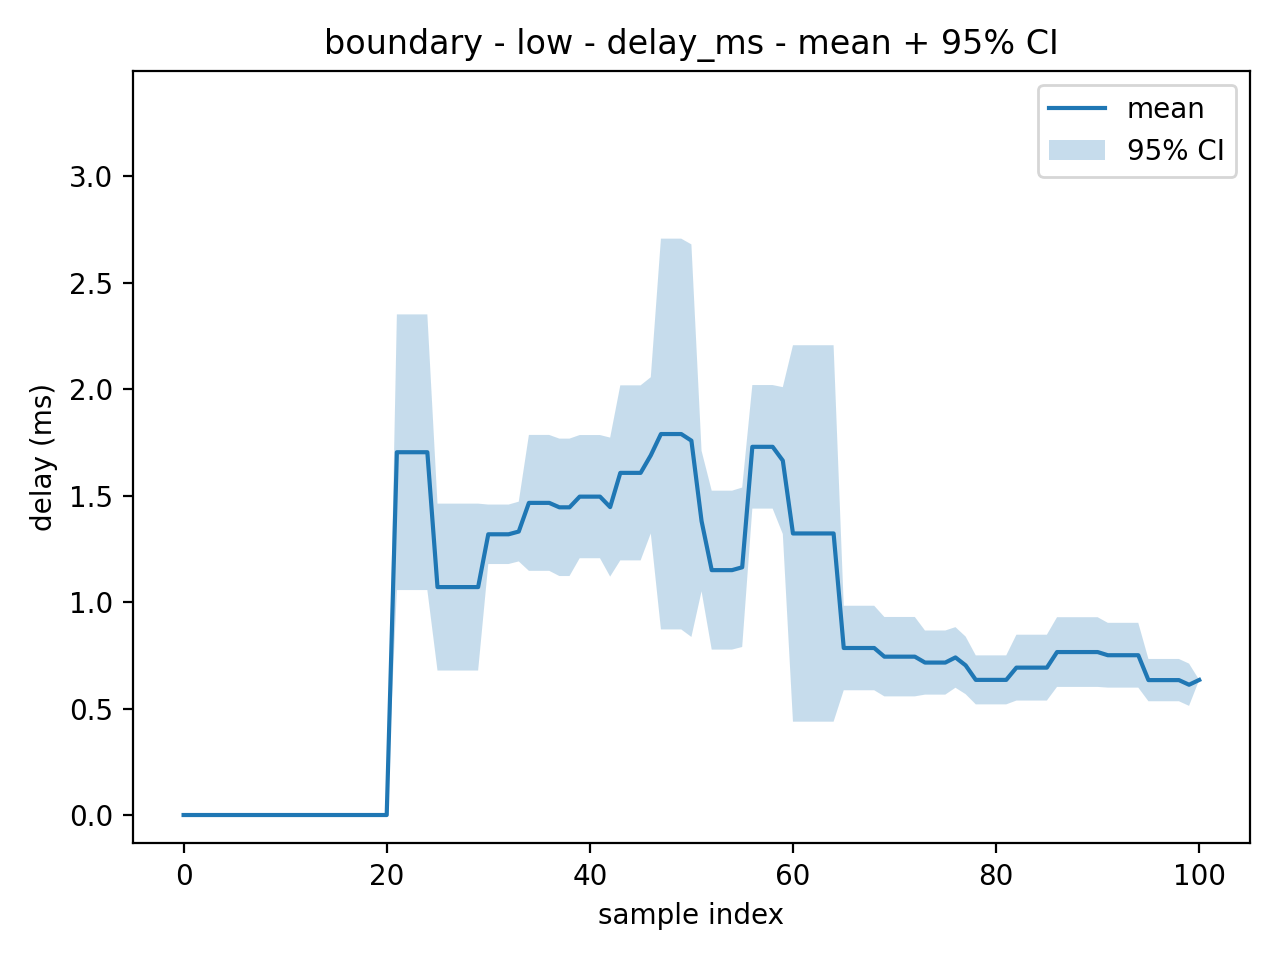
\includegraphics[width=\linewidth]{
      pars_plots/ntpsec/_aggregated/boundary/low/delay_ms_mean_ci95.png
    }
    \caption{Scenario LOW}
  \end{subfigure}
  \hfill
  \begin{subfigure}
    {0.32\textwidth}
    \centering
    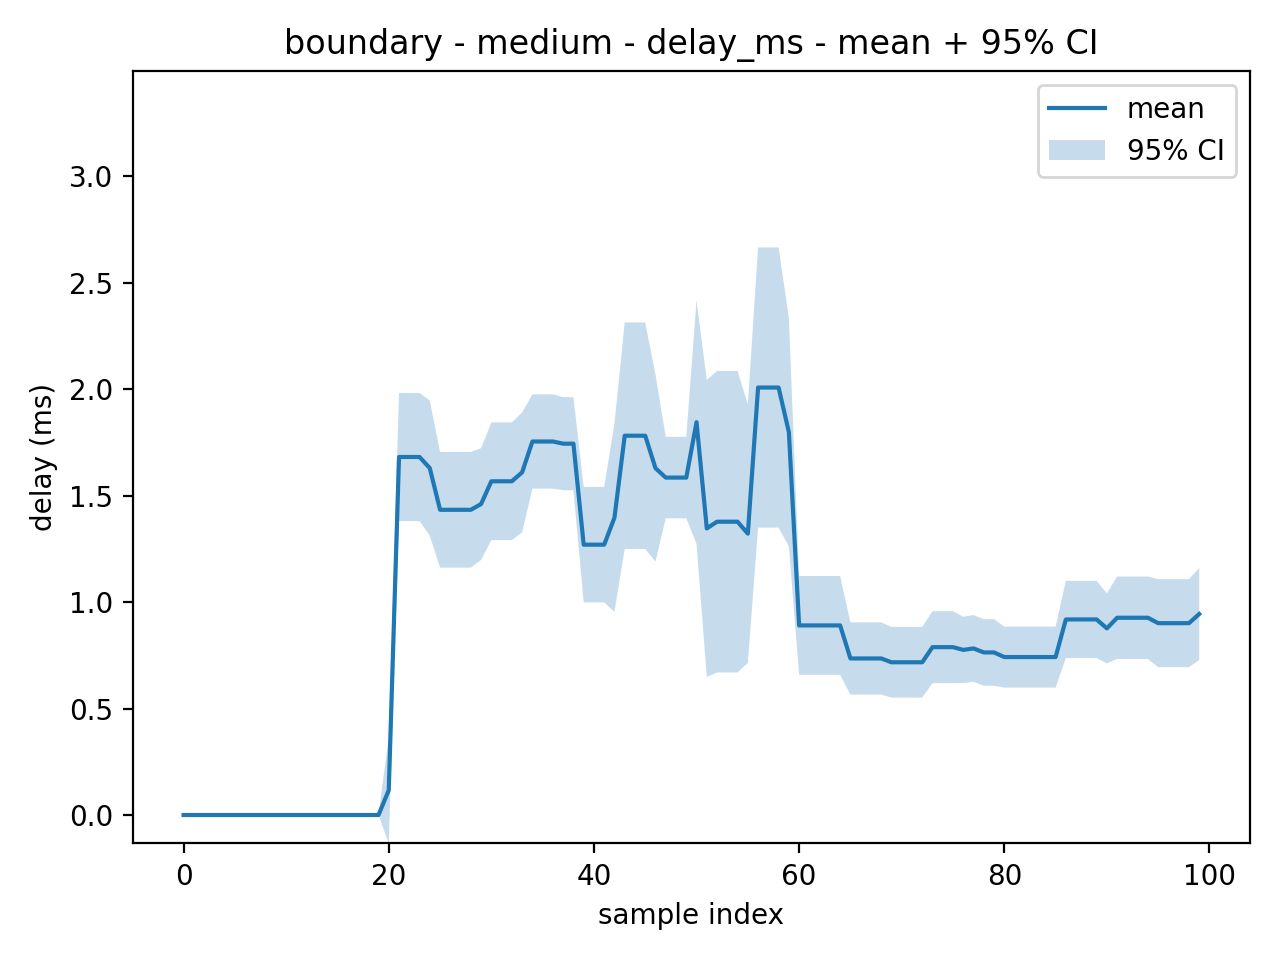
\includegraphics[width=\linewidth]{
      pars_plots/ntpsec/_aggregated/boundary/medium/delay_ms_mean_ci95.png
    }
    \caption{Scenario MEDIUM}
  \end{subfigure}
  \hfill
  \begin{subfigure}
    {0.32\textwidth}
    \centering
    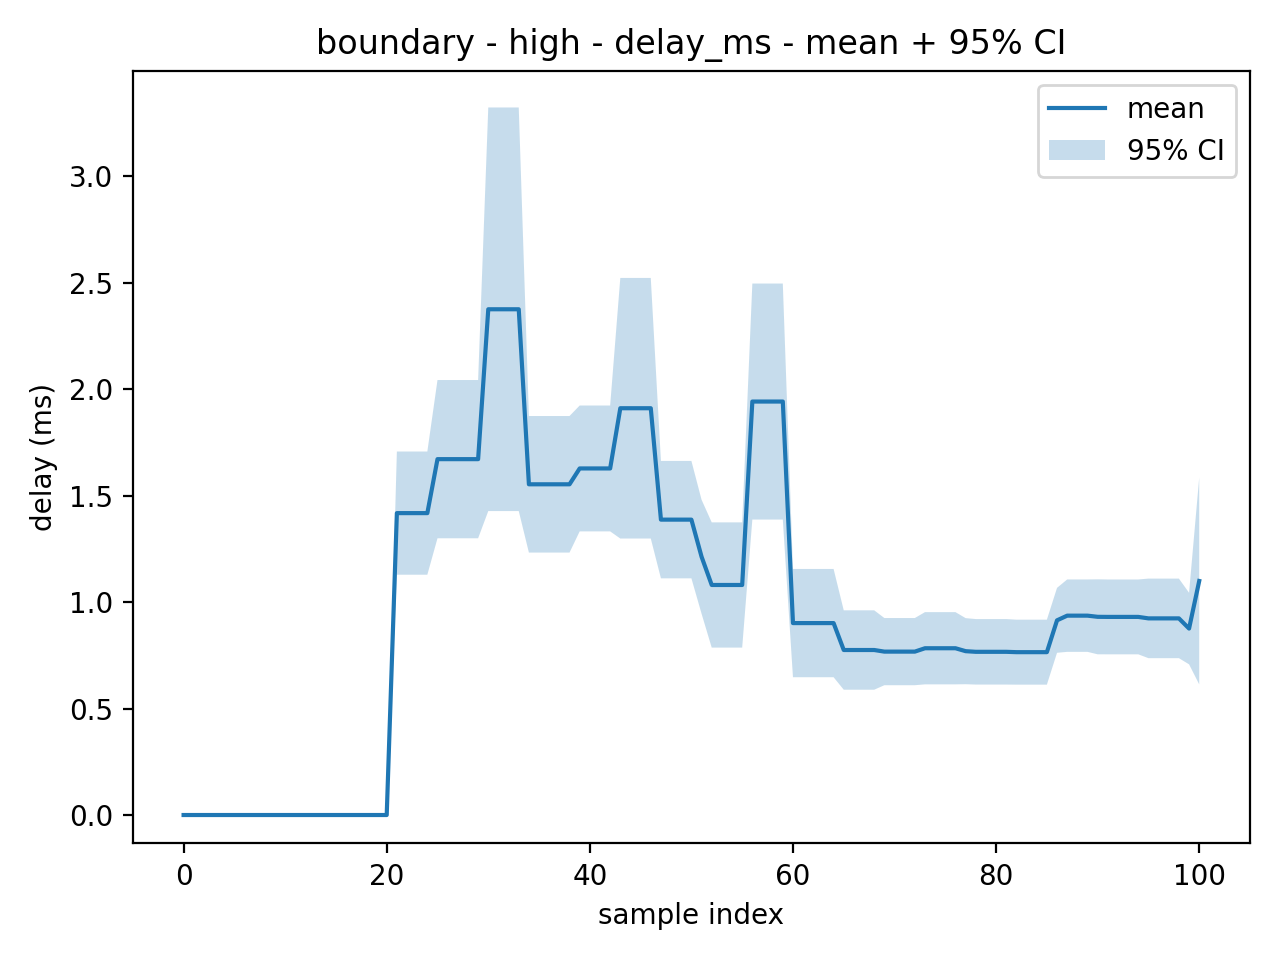
\includegraphics[width=\linewidth]{
      pars_plots/ntpsec/_aggregated/boundary/high/delay_ms_mean_ci95.png
    }
    \caption{Scenario HIGH}
  \end{subfigure}

  \caption{Media con intervallo di confidenza al 95\% - nodo: \texttt{boundary} metrica:
  \texttt{delay}}
  \label{fig:scenario_comparison}
\end{figure}
\begin{figure}[H]
  \centering

  \begin{subfigure}
    {0.32\textwidth}
    \centering
    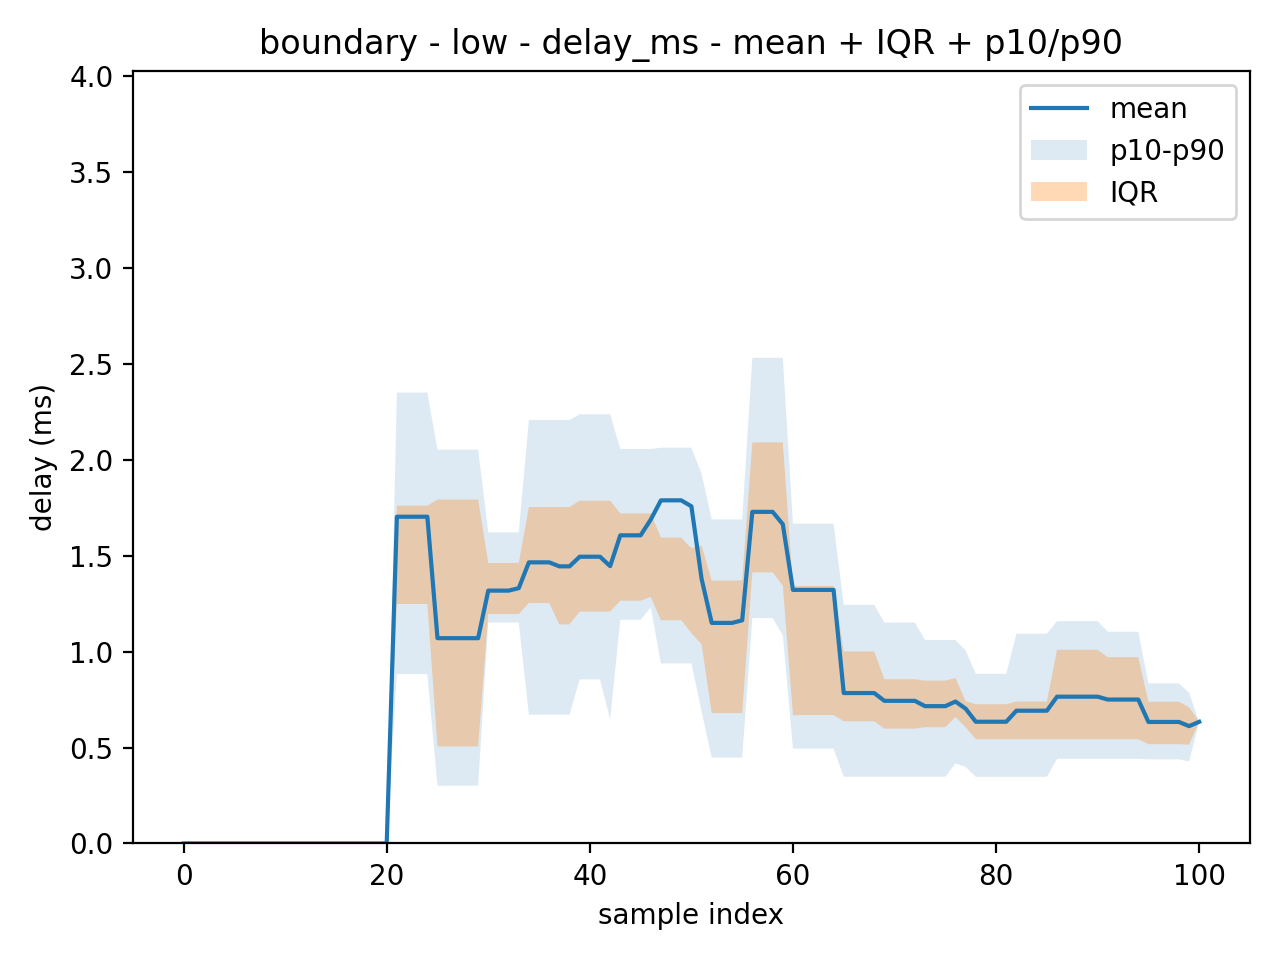
\includegraphics[width=\linewidth]{
      pars_plots/ntpsec/_aggregated/boundary/low/delay_ms_mean_iqr_p10_p90.png
    }
    \caption{Scenario LOW}
  \end{subfigure}
  \hfill
  \begin{subfigure}
    {0.32\textwidth}
    \centering
    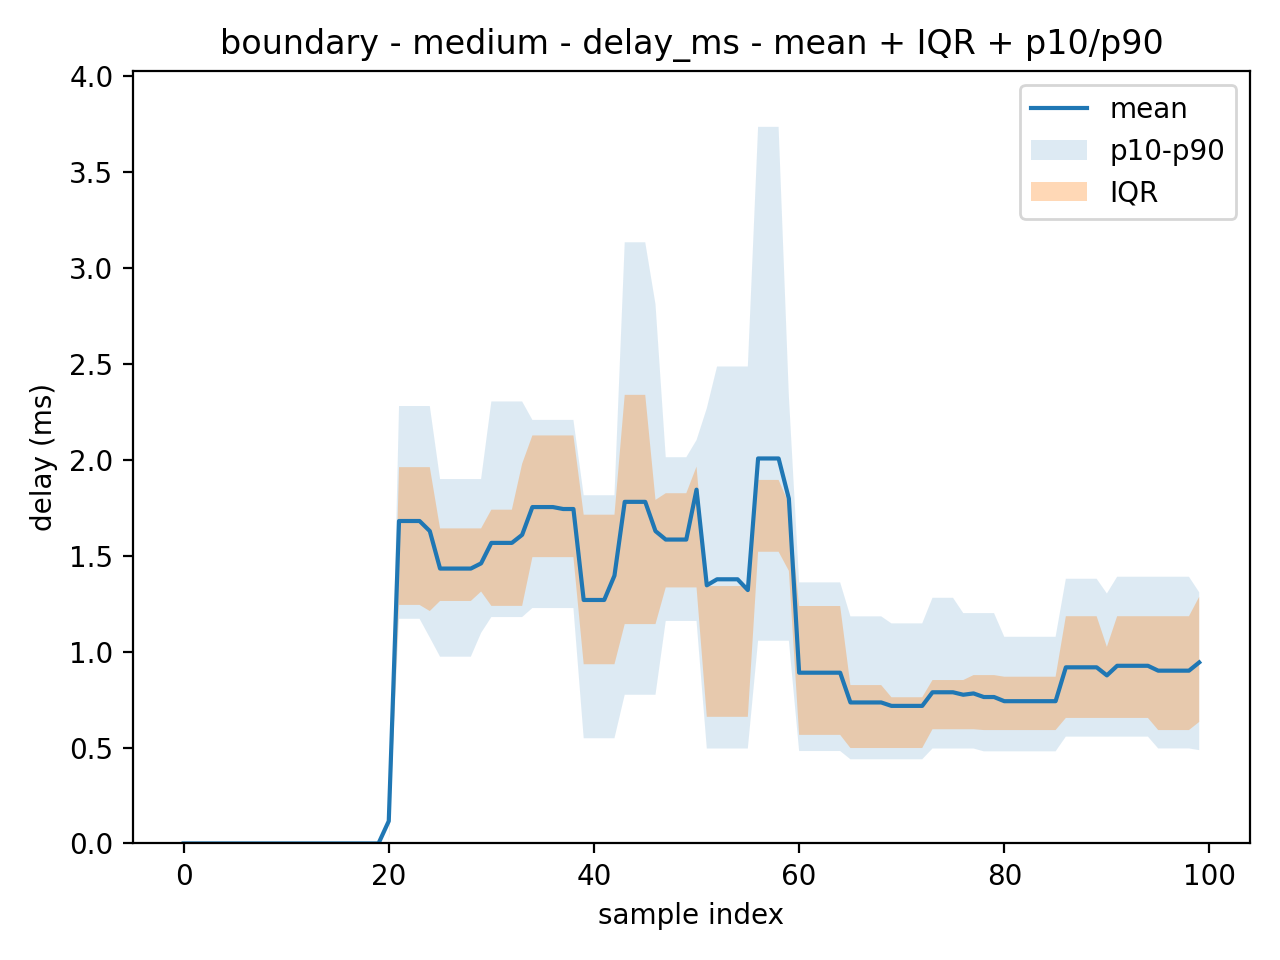
\includegraphics[width=\linewidth]{
      pars_plots/ntpsec/_aggregated/boundary/medium/delay_ms_mean_iqr_p10_p90.png
    }
    \caption{Scenario MEDIUM}
  \end{subfigure}
  \hfill
  \begin{subfigure}
    {0.32\textwidth}
    \centering
    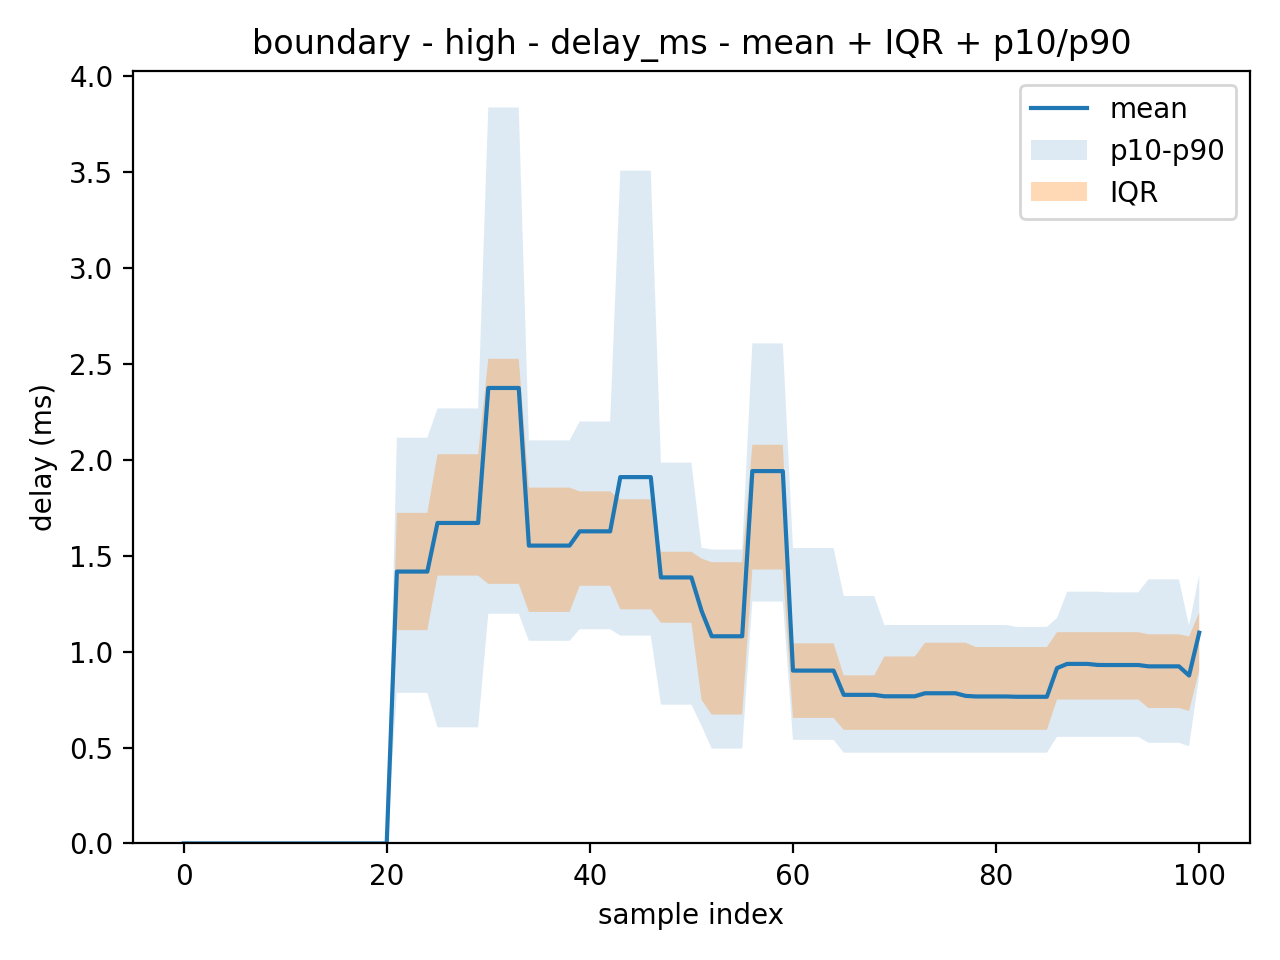
\includegraphics[width=\linewidth]{
      pars_plots/ntpsec/_aggregated/boundary/high/delay_ms_mean_iqr_p10_p90.png
    }
    \caption{Scenario HIGH}
  \end{subfigure}

  \caption{Media con banda interquartile e banda p10-p90 - nodo: \texttt{boundary}
  metrica: \texttt{delay}}
  \label{fig:scenario_comparison}
\end{figure}

\hrule

\begin{figure}[H]
  \centering

  \begin{subfigure}
    {0.32\textwidth}
    \centering
    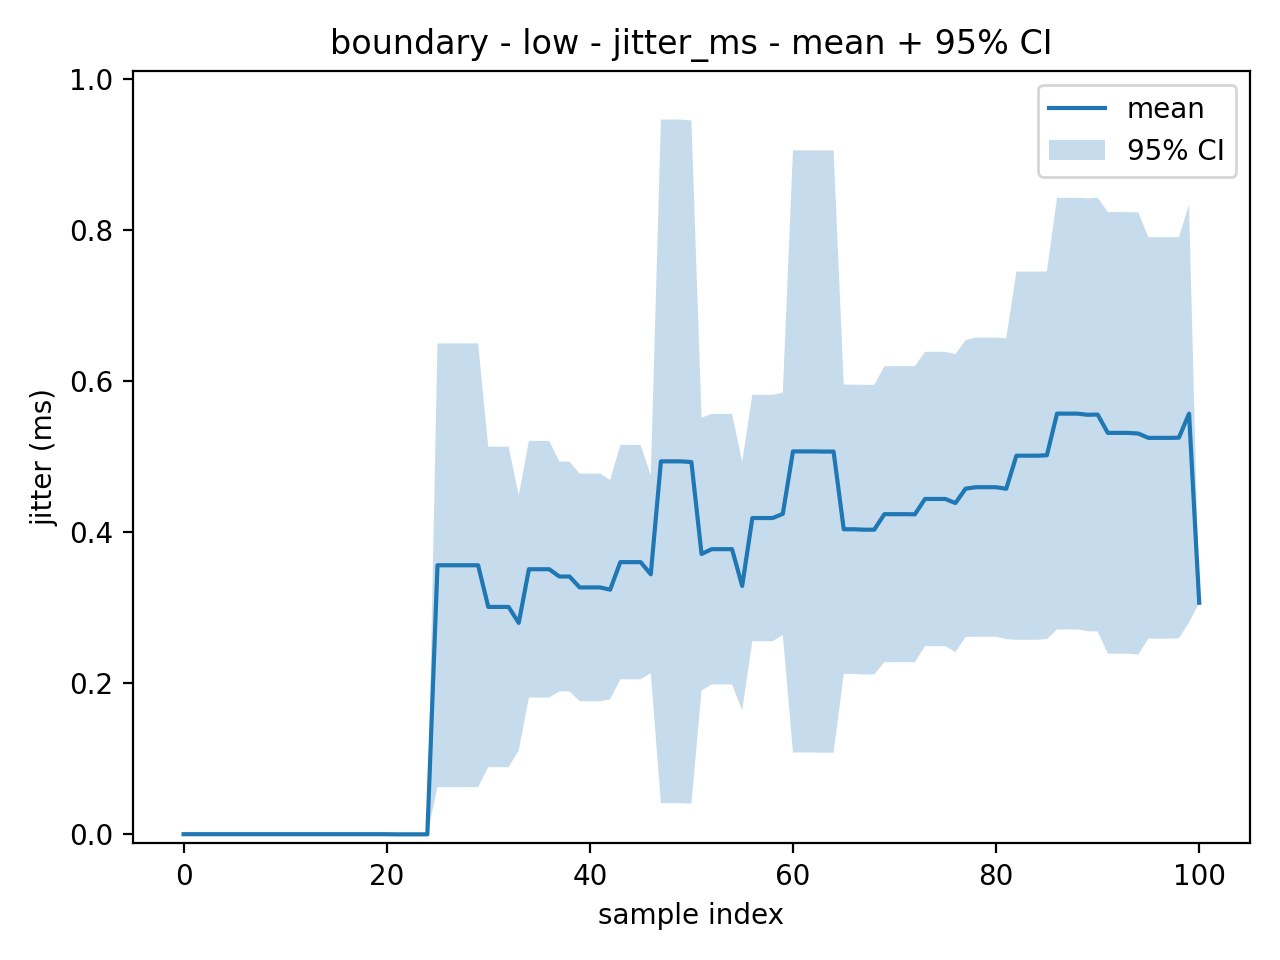
\includegraphics[width=\linewidth]{
      pars_plots/ntpsec/_aggregated/boundary/low/jitter_ms_mean_ci95.png
    }
    \caption{Scenario LOW}
  \end{subfigure}
  \hfill
  \begin{subfigure}
    {0.32\textwidth}
    \centering
    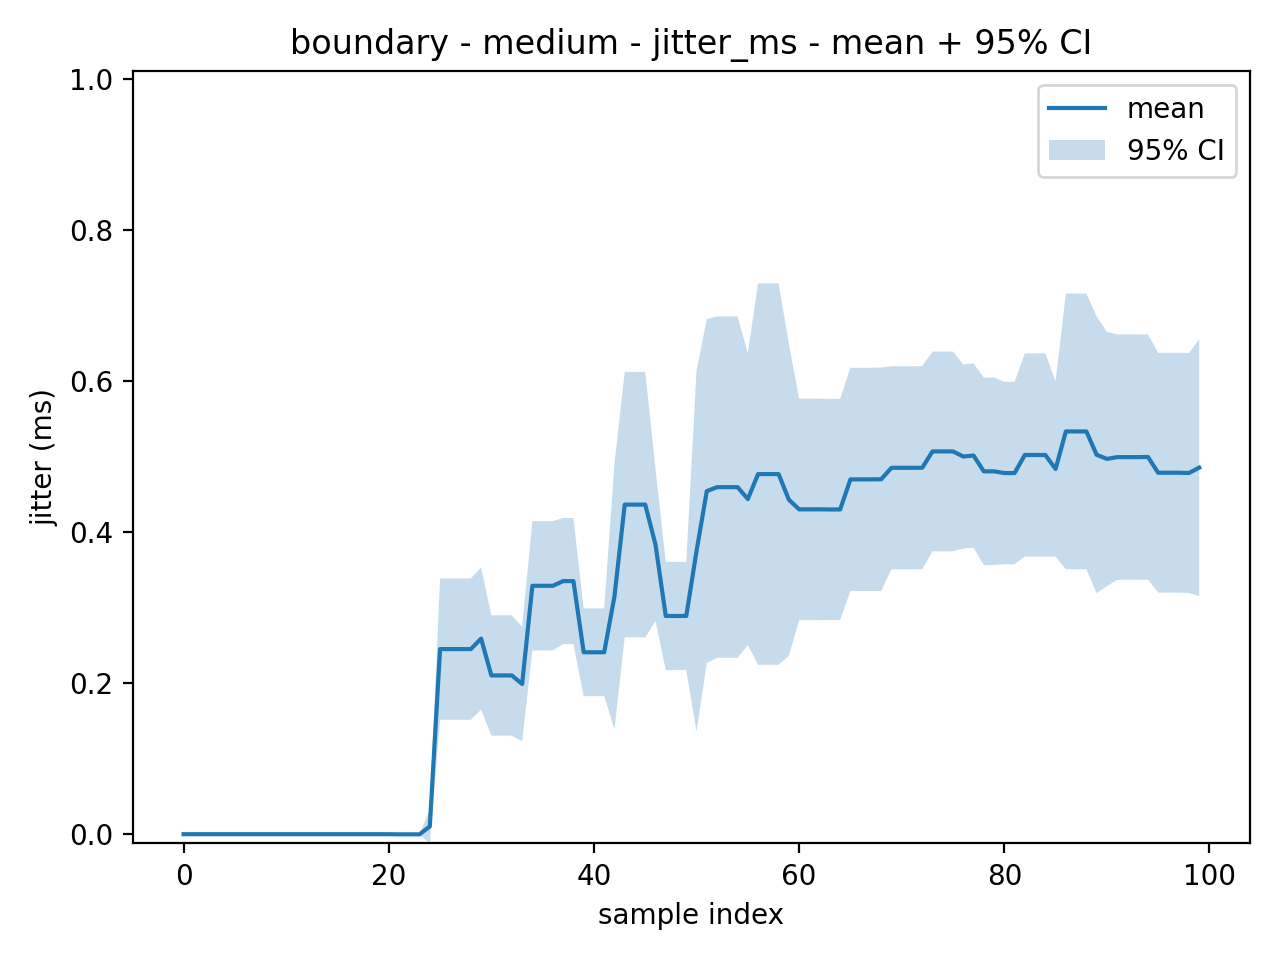
\includegraphics[width=\linewidth]{
      pars_plots/ntpsec/_aggregated/boundary/medium/jitter_ms_mean_ci95.png
    }
    \caption{Scenario MEDIUM}
  \end{subfigure}
  \hfill
  \begin{subfigure}
    {0.32\textwidth}
    \centering
    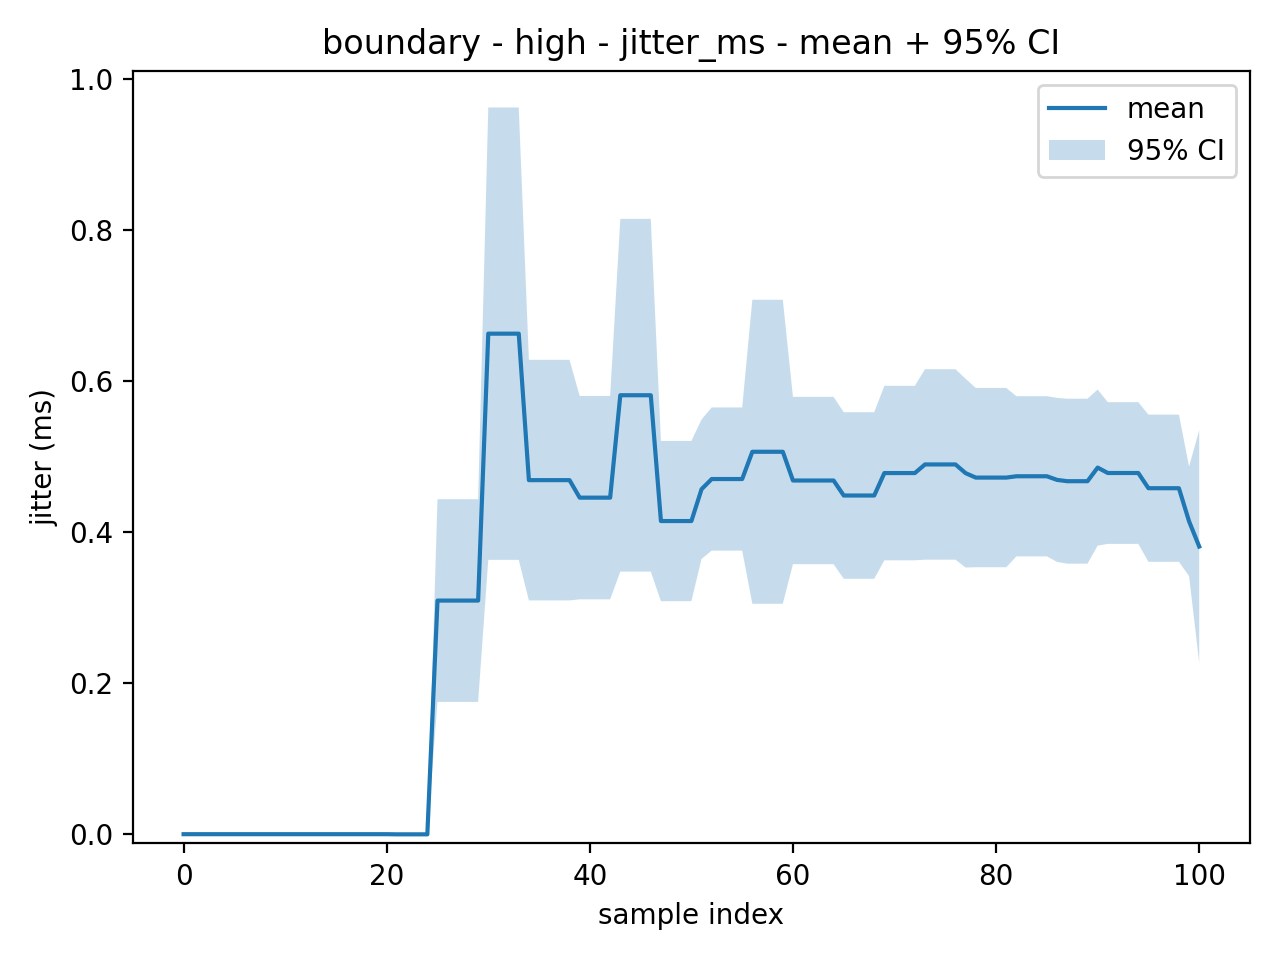
\includegraphics[width=\linewidth]{
      pars_plots/ntpsec/_aggregated/boundary/high/jitter_ms_mean_ci95.png
    }
    \caption{Scenario HIGH}
  \end{subfigure}

  \caption{Media con intervallo di confidenza al 95\% - nodo: \texttt{boundary} metrica:
  \texttt{delay}}
  \label{fig:scenario_comparison}
\end{figure}
\begin{figure}[H]
  \centering

  \begin{subfigure}
    {0.32\textwidth}
    \centering
    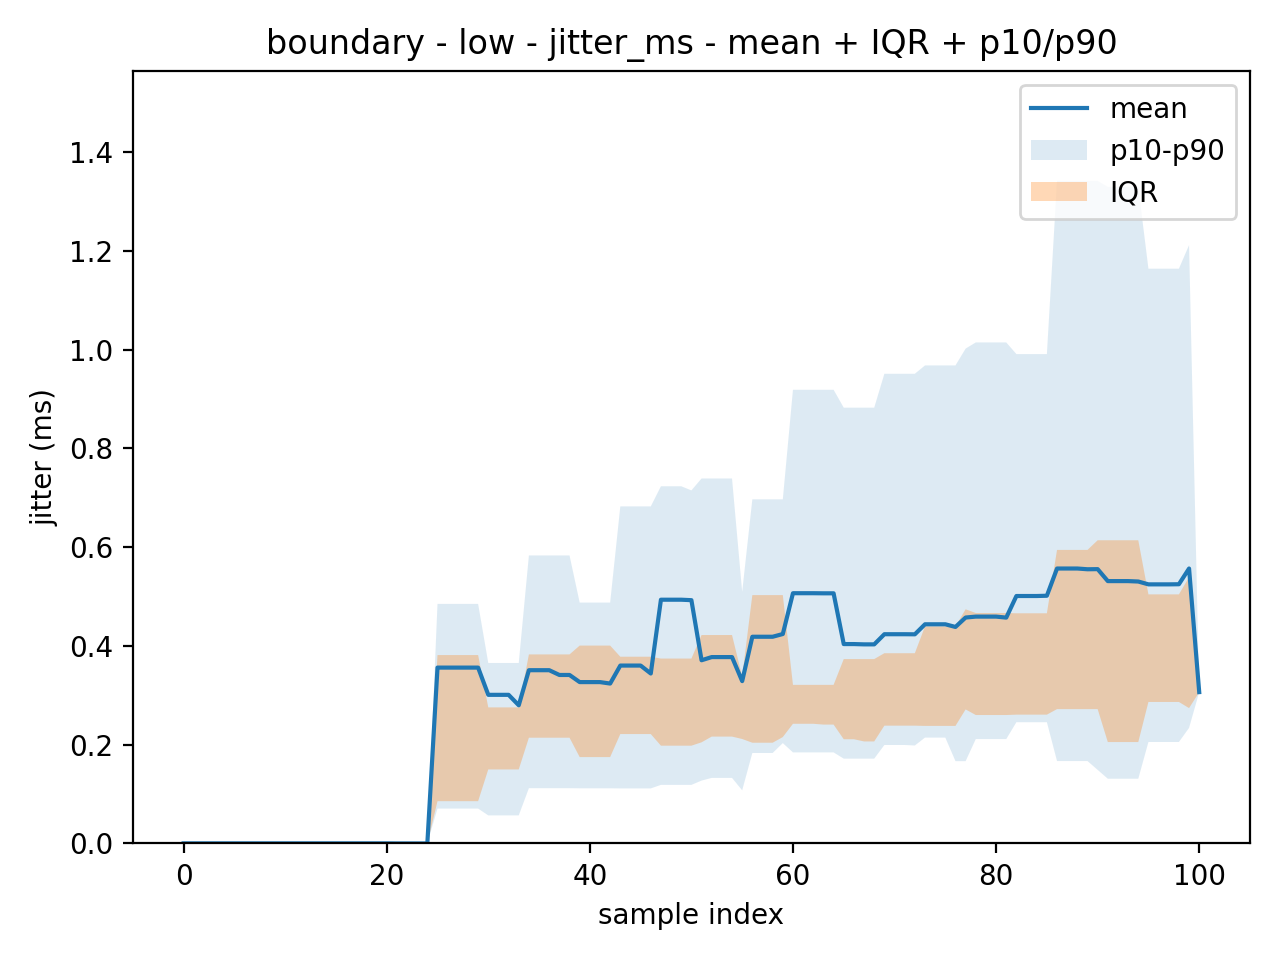
\includegraphics[width=\linewidth]{
      pars_plots/ntpsec/_aggregated/boundary/low/jitter_ms_mean_iqr_p10_p90.png
    }
    \caption{Scenario LOW}
  \end{subfigure}
  \hfill
  \begin{subfigure}
    {0.32\textwidth}
    \centering
    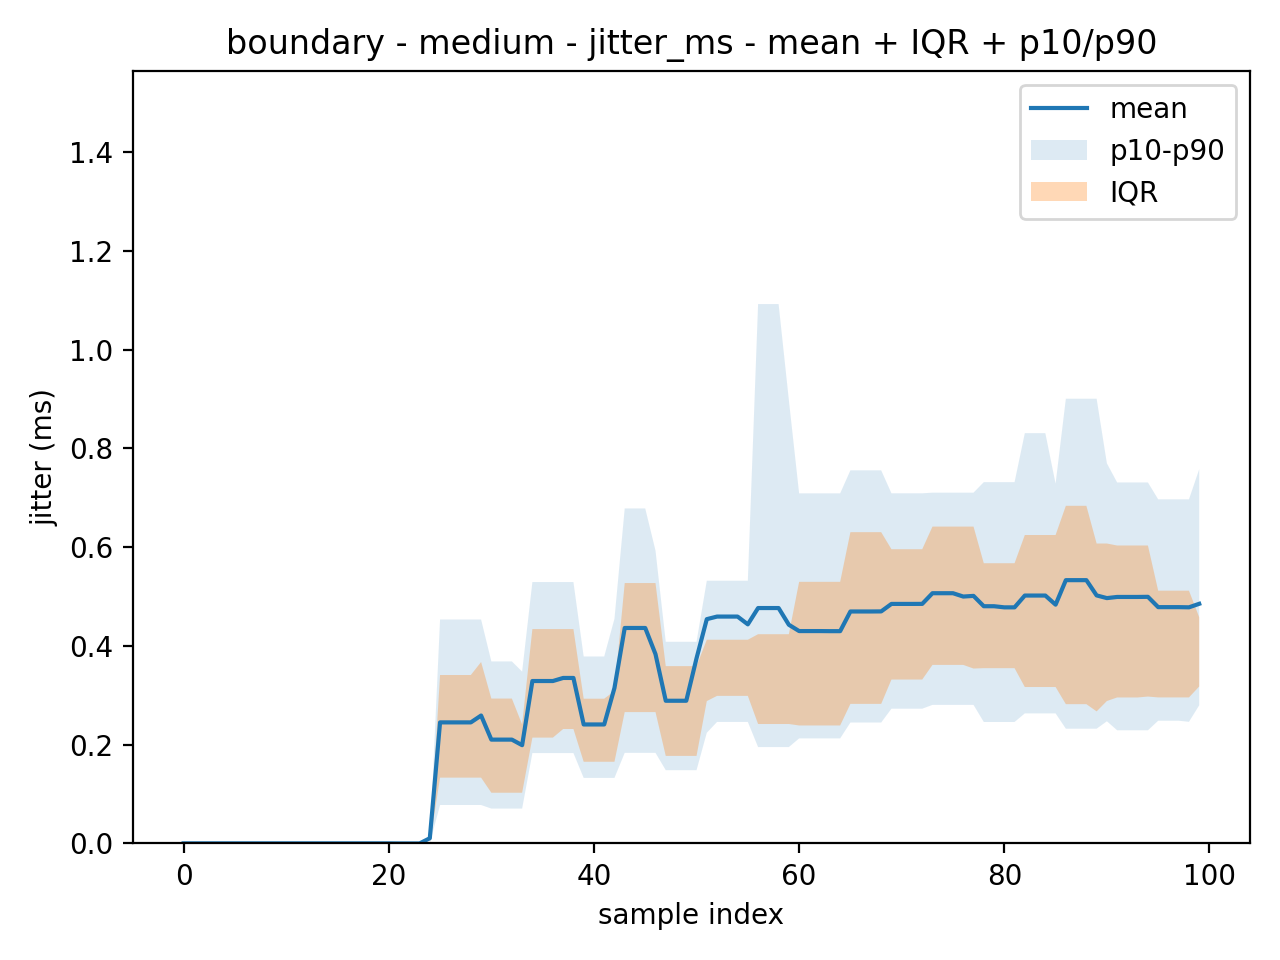
\includegraphics[width=\linewidth]{
      pars_plots/ntpsec/_aggregated/boundary/medium/jitter_ms_mean_iqr_p10_p90.png
    }
    \caption{Scenario MEDIUM}
  \end{subfigure}
  \hfill
  \begin{subfigure}
    {0.32\textwidth}
    \centering
    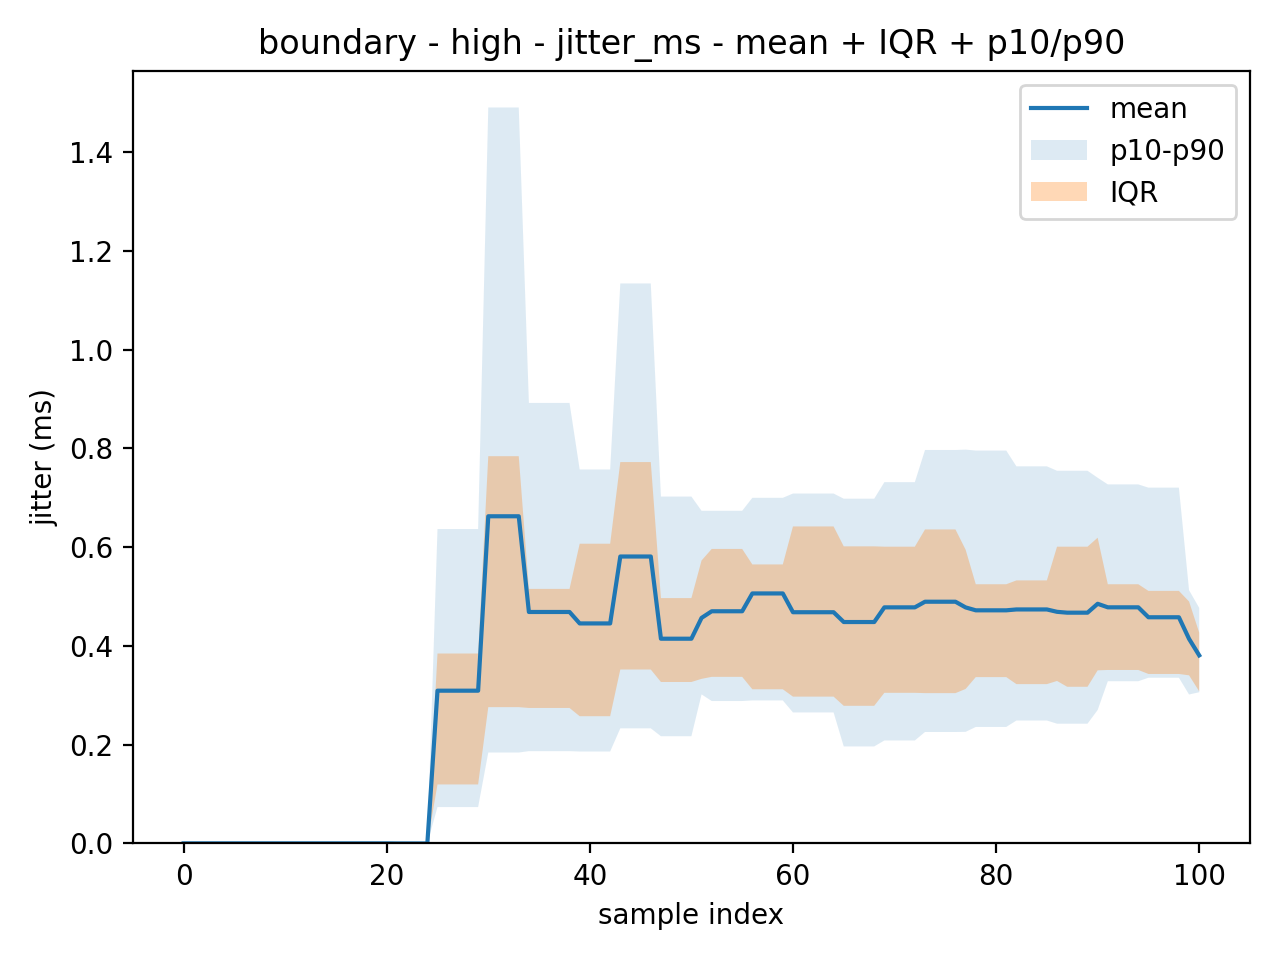
\includegraphics[width=\linewidth]{
      pars_plots/ntpsec/_aggregated/boundary/high/jitter_ms_mean_iqr_p10_p90.png
    }
    \caption{Scenario HIGH}
  \end{subfigure}

  \caption{Media con banda interquartile e banda p10-p90 - nodo: \texttt{boundary}
  metrica: \texttt{delay}}
  \label{fig:scenario_comparison}
\end{figure}

\hrule

\begin{figure}[H]
  \centering

  \begin{subfigure}
    {0.32\textwidth}
    \centering
    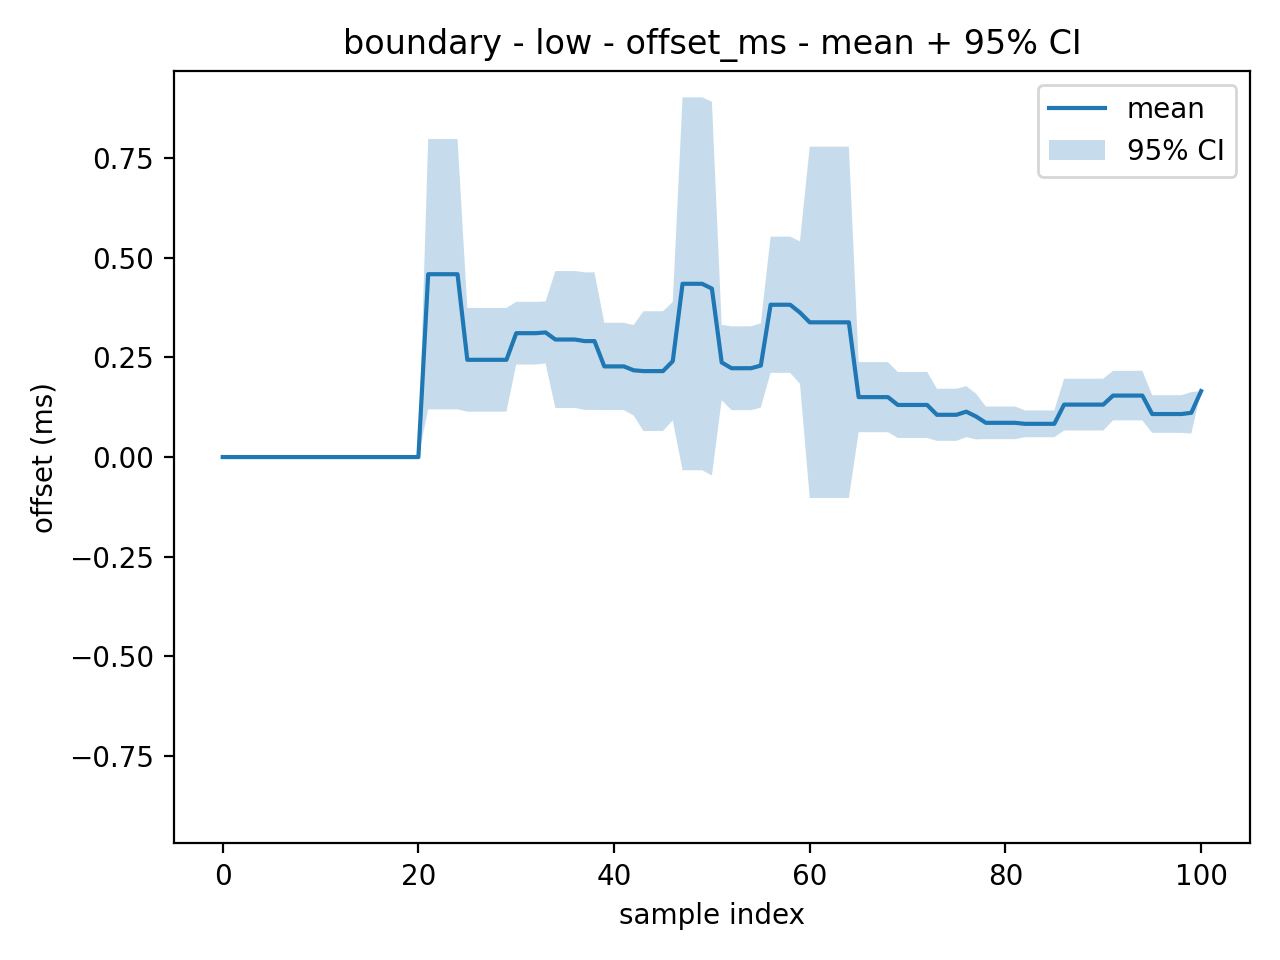
\includegraphics[width=\linewidth]{
      pars_plots/ntpsec/_aggregated/boundary/low/offset_ms_mean_ci95.png
    }
    \caption{Scenario LOW}
  \end{subfigure}
  \hfill
  \begin{subfigure}
    {0.32\textwidth}
    \centering
    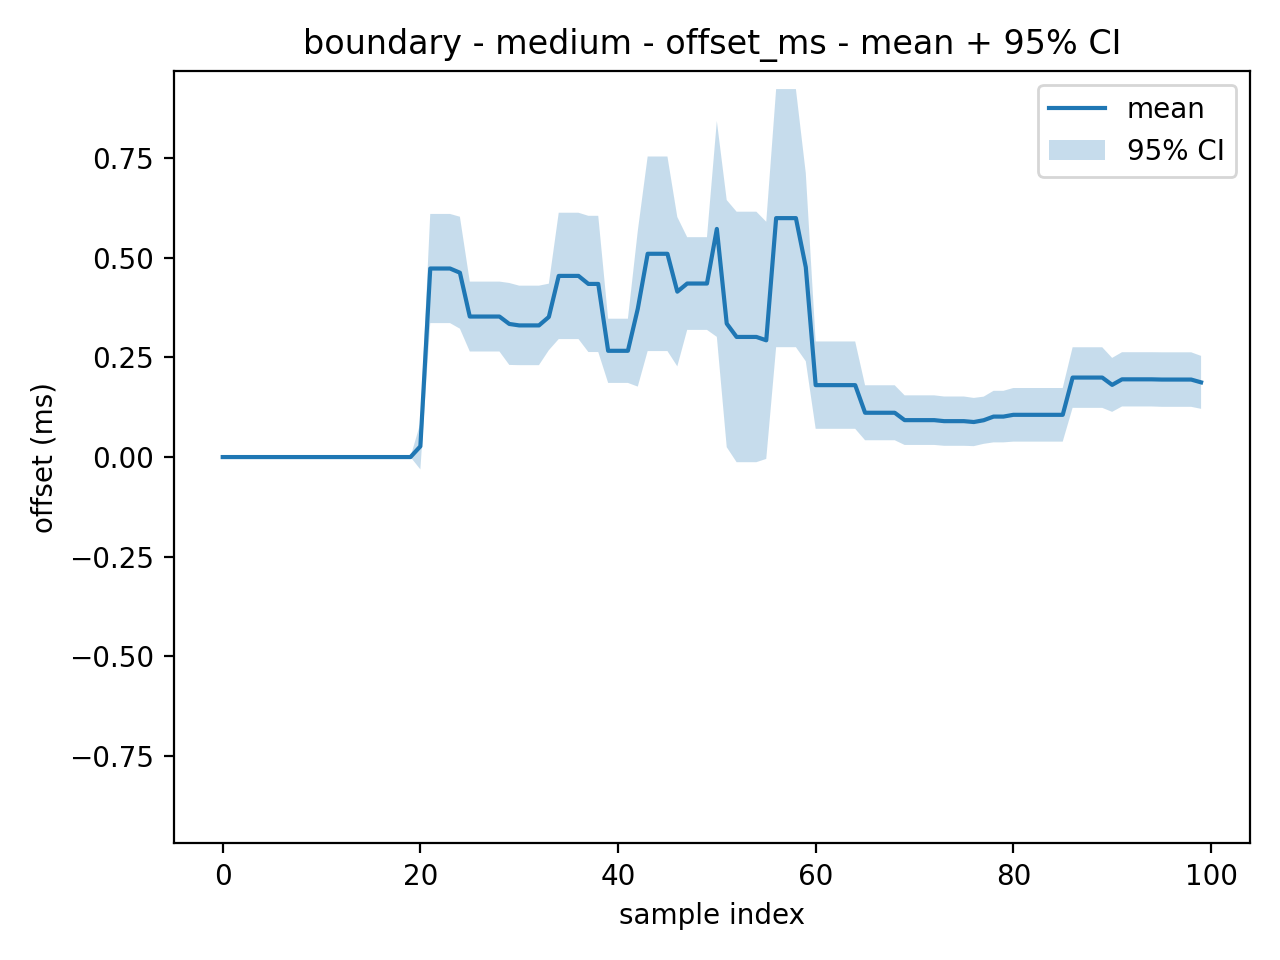
\includegraphics[width=\linewidth]{
      pars_plots/ntpsec/_aggregated/boundary/medium/offset_ms_mean_ci95.png
    }
    \caption{Scenario MEDIUM}
  \end{subfigure}
  \hfill
  \begin{subfigure}
    {0.32\textwidth}
    \centering
    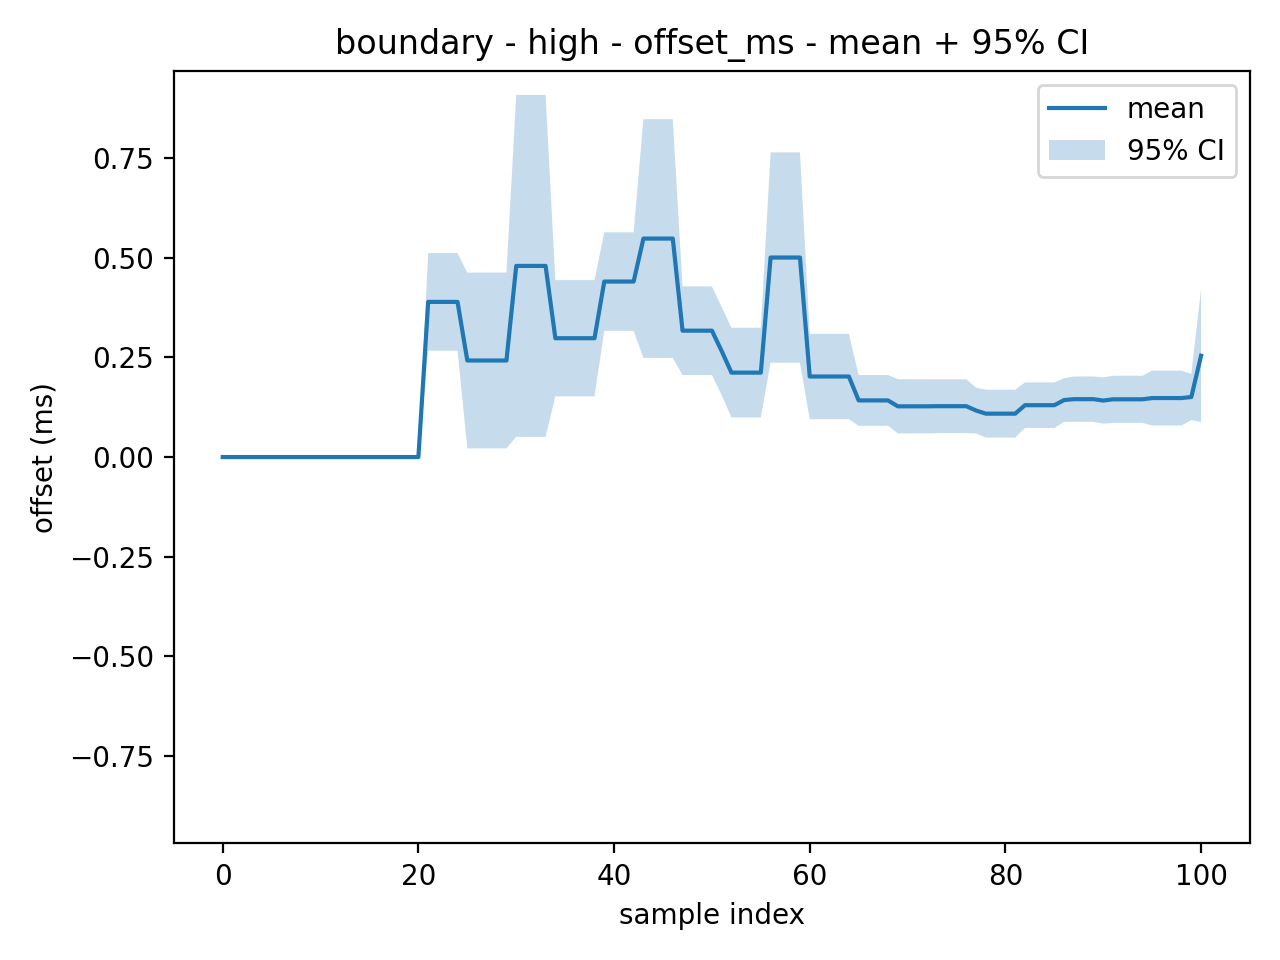
\includegraphics[width=\linewidth]{
      pars_plots/ntpsec/_aggregated/boundary/high/offset_ms_mean_ci95.png
    }
    \caption{Scenario HIGH}
  \end{subfigure}

  \caption{Media con intervallo di confidenza al 95\% - nodo: \texttt{boundary} metrica:
  \texttt{delay}}
  \label{fig:scenario_comparison}
\end{figure}
\begin{figure}[H]
  \centering

  \begin{subfigure}
    {0.32\textwidth}
    \centering
    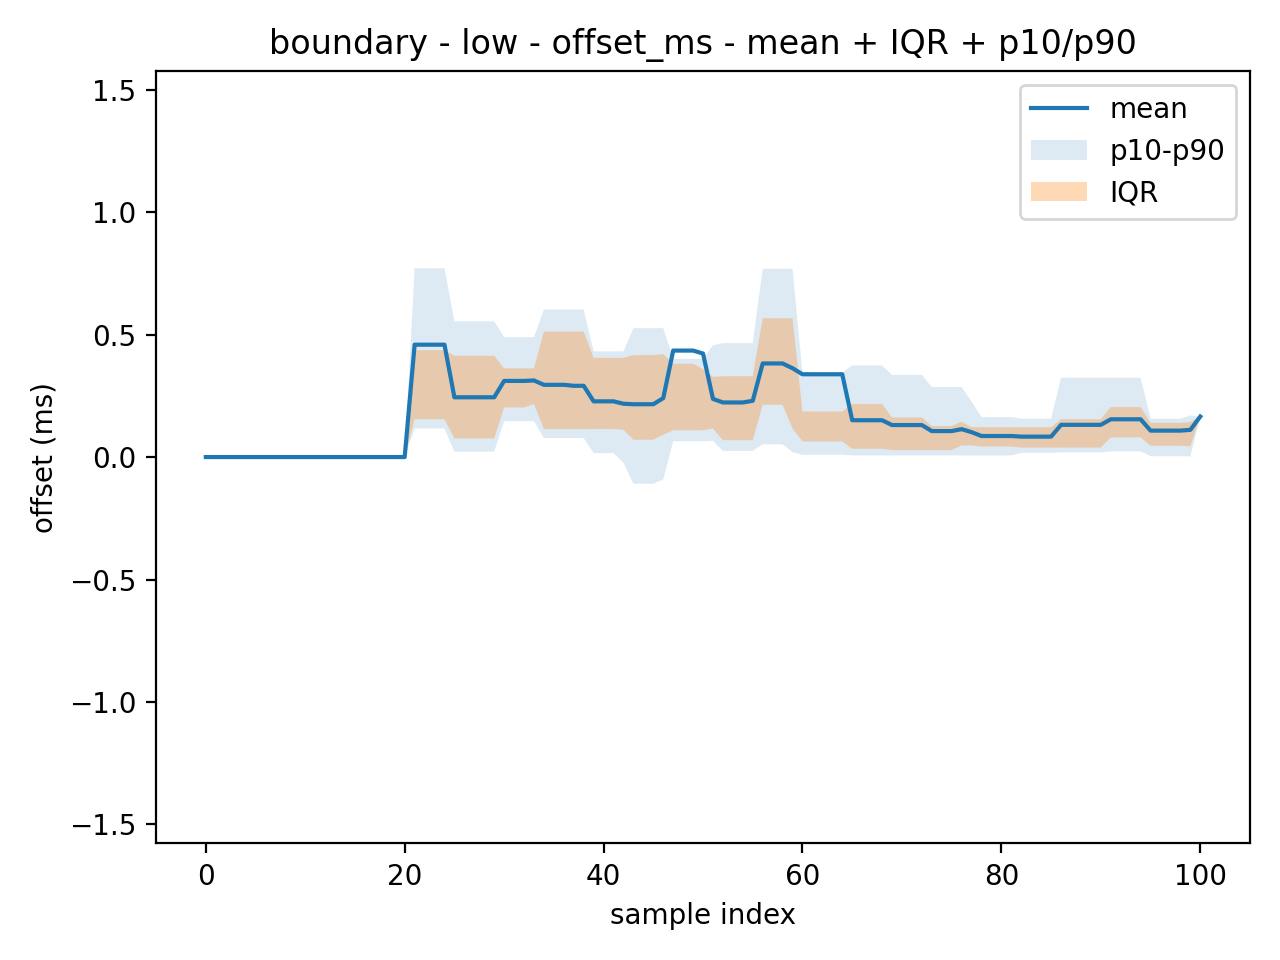
\includegraphics[width=\linewidth]{
      pars_plots/ntpsec/_aggregated/boundary/low/offset_ms_mean_iqr_p10_p90.png
    }
    \caption{Scenario LOW}
  \end{subfigure}
  \hfill
  \begin{subfigure}
    {0.32\textwidth}
    \centering
    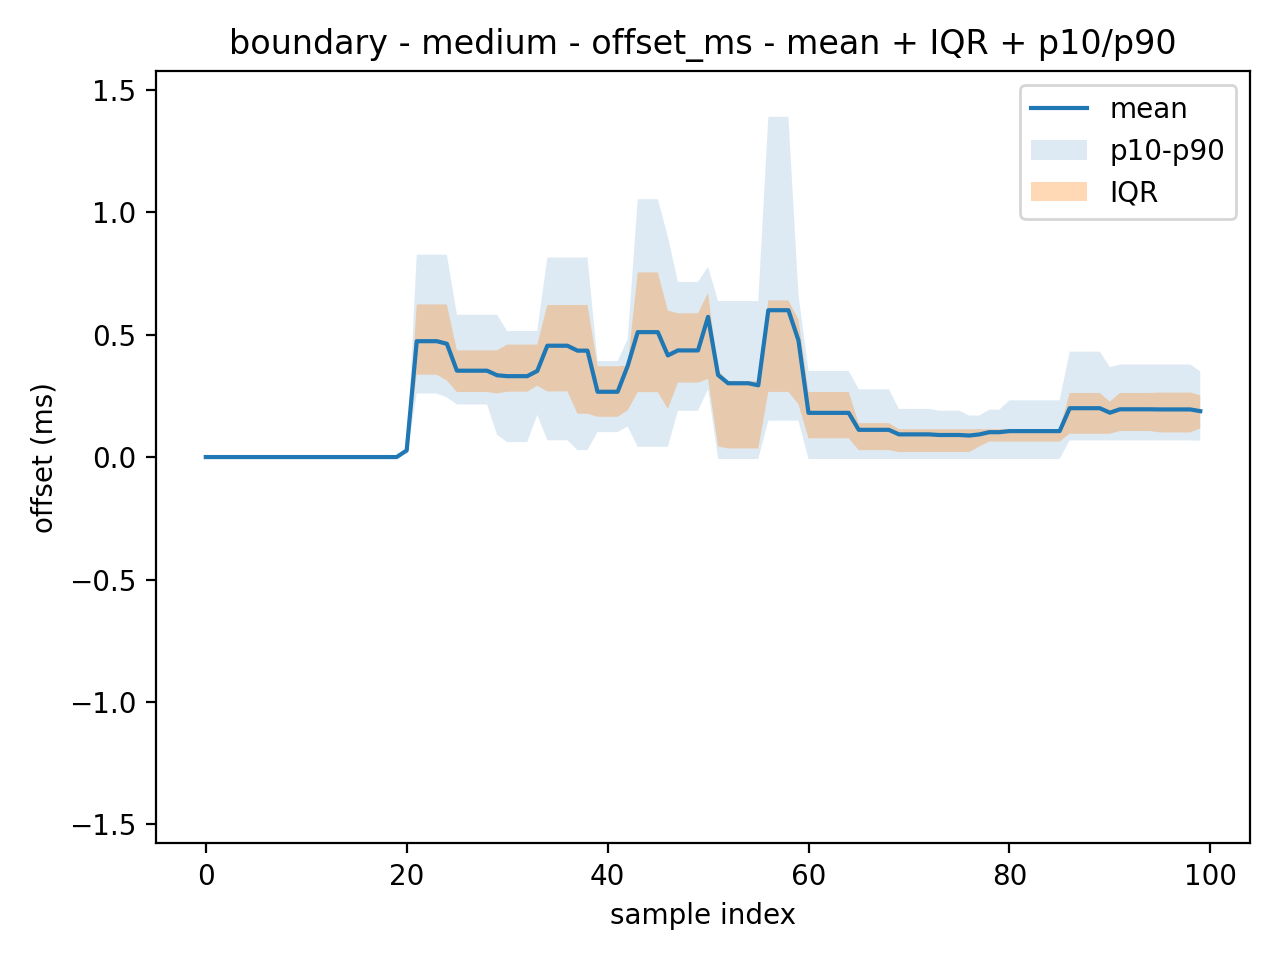
\includegraphics[width=\linewidth]{
      pars_plots/ntpsec/_aggregated/boundary/medium/offset_ms_mean_iqr_p10_p90.png
    }
    \caption{Scenario MEDIUM}
  \end{subfigure}
  \hfill
  \begin{subfigure}
    {0.32\textwidth}
    \centering
    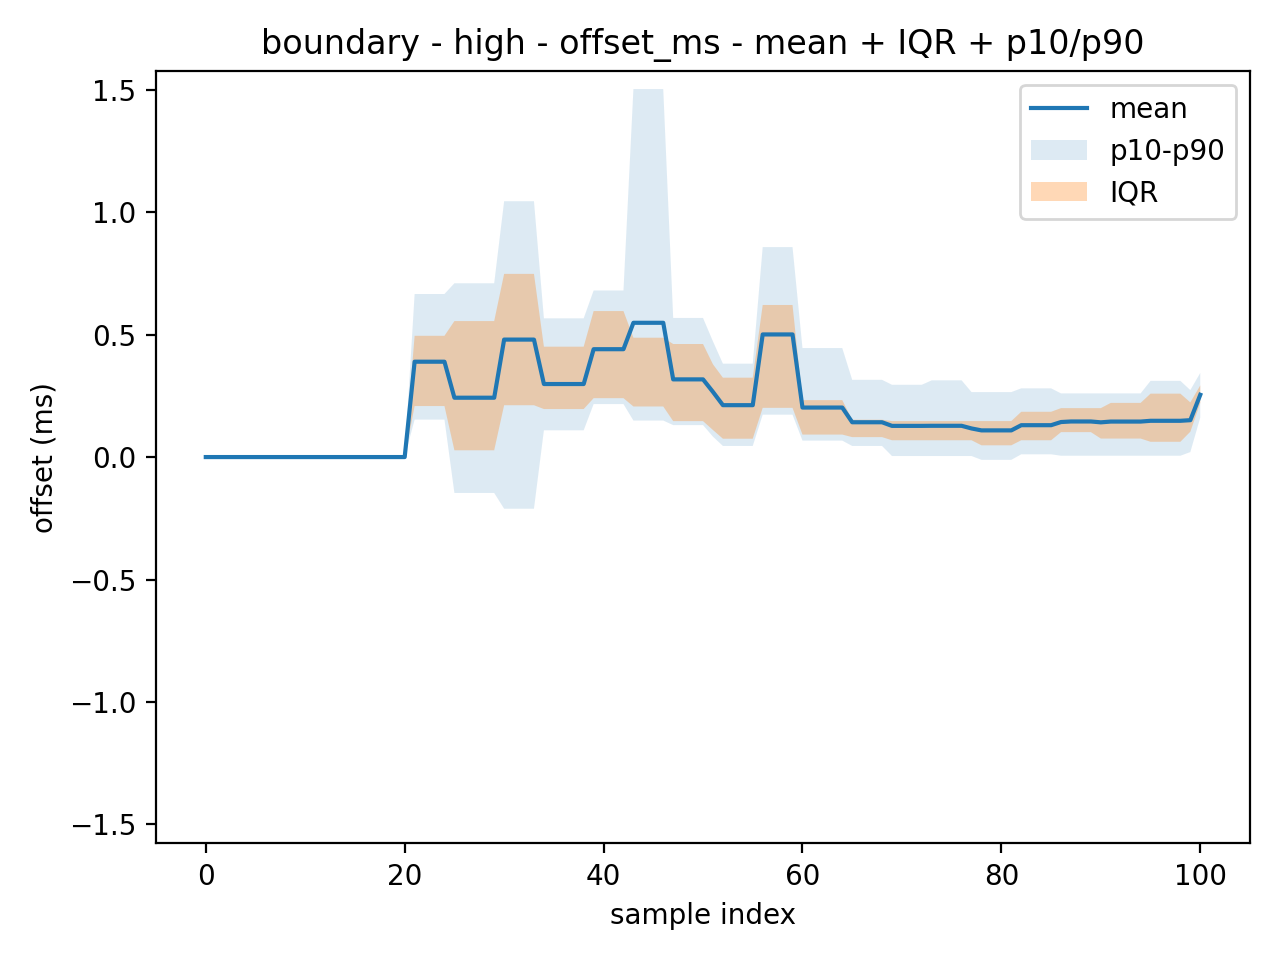
\includegraphics[width=\linewidth]{
      pars_plots/ntpsec/_aggregated/boundary/high/offset_ms_mean_iqr_p10_p90.png
    }
    \caption{Scenario HIGH}
  \end{subfigure}

  \caption{Media con banda interquartile e banda p10-p90 - nodo: \texttt{boundary}
  metrica: \texttt{delay}}
  \label{fig:scenario_comparison}
\end{figure}

L’analisi delle metriche rilevate sul nodo boundary mostra un comportamento
sensibilmente diverso rispetto a quello osservato sul nodo client. Nei tre scenari
sperimentali, infatti, offset, jitter e delay mantengono valori dello stesso
ordine di grandezza e non evidenziano una crescita progressiva netta al crescere
della severità degli impairment di rete. Tale risultato risulta coerente con la configurazione
del testbed, nella quale il degrado è stato introdotto sul ramo downstream verso
il client, mentre il collegamento upstream tra server e boundary non è stato soggetto
allo stesso trattamento.

Per quanto riguarda il delay, i valori medi post-selezione sono pari a circa
1.080 ms nello scenario low, 1.139 ms nello scenario medium e 1.127 ms nello scenario
high. Anche in questo caso le variazioni sono modeste e non configurano un
cambio di regime. La dispersione associata alla metrica rimane dello stesso ordine
di grandezza nei tre scenari, a conferma del fatto che il comportamento del
boundary non è significativamente influenzato dagli impairment introdotti a
valle.

Un andamento analogo si osserva infine per il jitter. Infatti conferma ulteriormente
questo quadro di stabilità. I valori medi post-selezione risultano pari a circa
0.446 ms in low, 0.442 ms in medium e 0.473 ms in high. Le differenze tra i tre
scenari sono molto ridotte e non indicano una sensibilità marcata del nodo
boundary al progressivo aumento del degrado di rete. Anche la variabilità delle curve
aggregate resta limitata, suggerendo un comportamento regolare e sostanzialmente
omogeneo nei tre casi.

Come ultimo si ha l’offset, con i valori post-selezione che restano contenuti in tutti
gli scenari, con media pari a circa 0.204 ms nel caso low, 0.254 ms nel caso medium
e 0.236 ms nel caso high. Si osserva quindi una lieve variazione tra gli scenari,
ma non un andamento monotono né un incremento tale da suggerire un peggioramento strutturale
della sincronizzazione sul boundary. Anche la dispersione resta complessivamente
contenuta, senza evidenza di un allargamento sistematico delle bande di variabilità.

Nel complesso, i risultati ottenuti sul boundary non mostrano un degrado netto e
progressivo al crescere della severità dello scenario sperimentale. Le differenze
osservate tra low, medium e high risultano contenute e prive di una tendenza
sistematica, a differenza di quanto rilevato sul client. I dati confermano
quindi che l’impatto principale degli impairment introdotti nella rete si
manifesta sul nodo downstream, mentre il boundary mantiene un comportamento sostanzialmente
stabile.

\section{\texttt{ptp4l}}
L’analisi dei dati relativa al demone \texttt{\textbf{ptp4l}} è articolata in
funzione dei nodi della topologia sui quali sono state rilevate le metriche di
interesse. In particolare, l’attenzione è rivolta ai nodi \texttt{clientptp} e \texttt{boundary},
per i quali sono disponibili misurazioni direttamente riconducibili al comportamento
del protocollo in termini di sincronizzazione e ritardo.

Il nodo \texttt{servergm}, al contrario, non fornisce una serie di metriche
comparabili a quelle osservate sugli altri nodi, poiché il relativo output è limitato
essenzialmente allo stato di inizializzazione del demone e alla selezione del clock
locale come \texttt{best master}. Per tale ragione, esso non viene incluso
nell’analisi quantitativa presentata in questa sezione.

Anche nel caso di \texttt{\textbf{ptp4l}}, gli impairment di rete introdotti
mediante \texttt{tc/netem} sono applicati sul ramo \texttt{downstream} a valle
del nodo \texttt{boundary}. Ne consegue che il confronto tra scenari assume un
significato diverso a seconda del nodo osservato: nel caso del \texttt{clientptp},
le metriche possono riflettere in modo diretto il degrado introdotto sulla rete,
mentre nel caso del \texttt{boundary} ci si attende, in linea teorica, un impatto
più contenuto, poiché il collegamento verso il nodo di riferimento non è quello
direttamente soggetto agli impairment configurati.

Alla luce di ciò, l’analisi viene sviluppata separatamente per i nodi \texttt{clientptp}
e \texttt{boundary}, così da evidenziare sia gli effetti diretti del degrado di
rete sul nodo terminale, sia l’eventuale presenza di variazioni indirette sul nodo
intermedio della topologia.

\subsection{\texttt{clientptp}}
Nel caso del nodo \texttt{clientptp}, l’analisi quantitativa delle metriche non può
essere estesa in modo uniforme a tutti e tre gli scenari sperimentali. In
particolare, nello scenario \texttt{high} non viene raggiunta una condizione
operativa stabile tale da produrre una serie di campioni utilizzabile per il
calcolo delle metriche considerate. Per tale ragione, i confronti quantitativi
sul nodo \texttt{clientptp} sono necessariamente limitati ai soli scenari \texttt{low}
e \texttt{medium}.

Nello scenario \texttt{high} non si raggiunge una condizione di sincronizzazione
stabile: il log mostra ripetute selezioni del clock locale come miglior master e un
solo tentativo transitorio di passaggio verso un master esterno, seguito
tuttavia da ritorno allo stato di \texttt{LISTENING}. L’assenza di campioni
numerici confrontabili nello scenario \texttt{high} rappresenta dunque un risultato
sperimentale, e segnala un livello di degrado tale da impedire la normale
operatività del client PTP. Il relativo output grezzo viene comunque richiamato a
supporto di tale evidenza qualitativa.

\subsubsection{Analisi metrica: \texttt{path Delay}}
\begin{figure}[H]
  \centering

  \begin{subfigure}
    {0.4\textwidth}
    \centering
    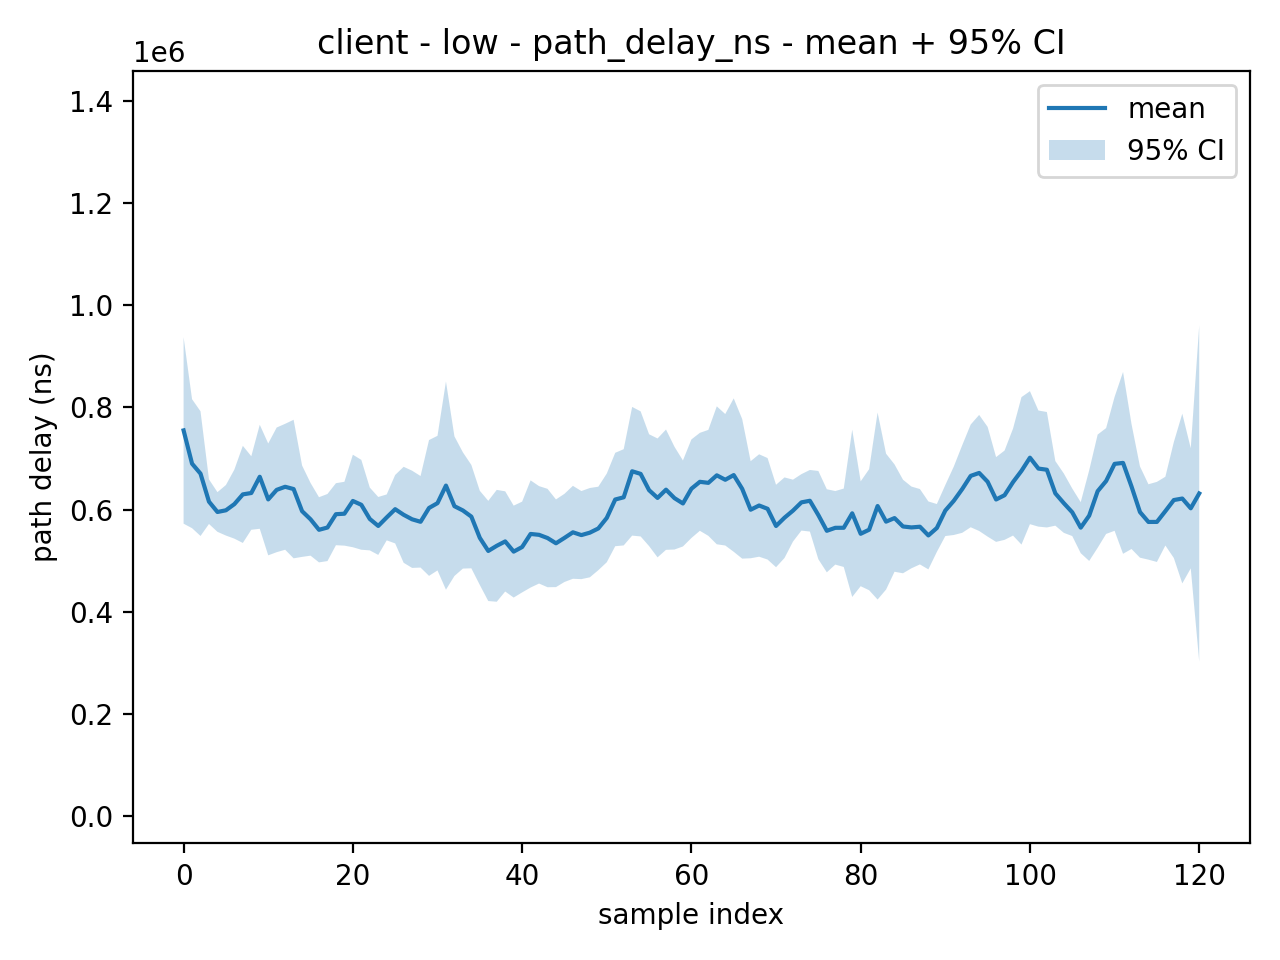
\includegraphics[width=\linewidth]{
      pars_plots/ptp/_aggregated/client/low/path_delay_ns_mean_ci95.png
    }
    \caption{Scenario LOW}
  \end{subfigure}
  \hfill
  \begin{subfigure}
    {0.4\textwidth}
    \centering
    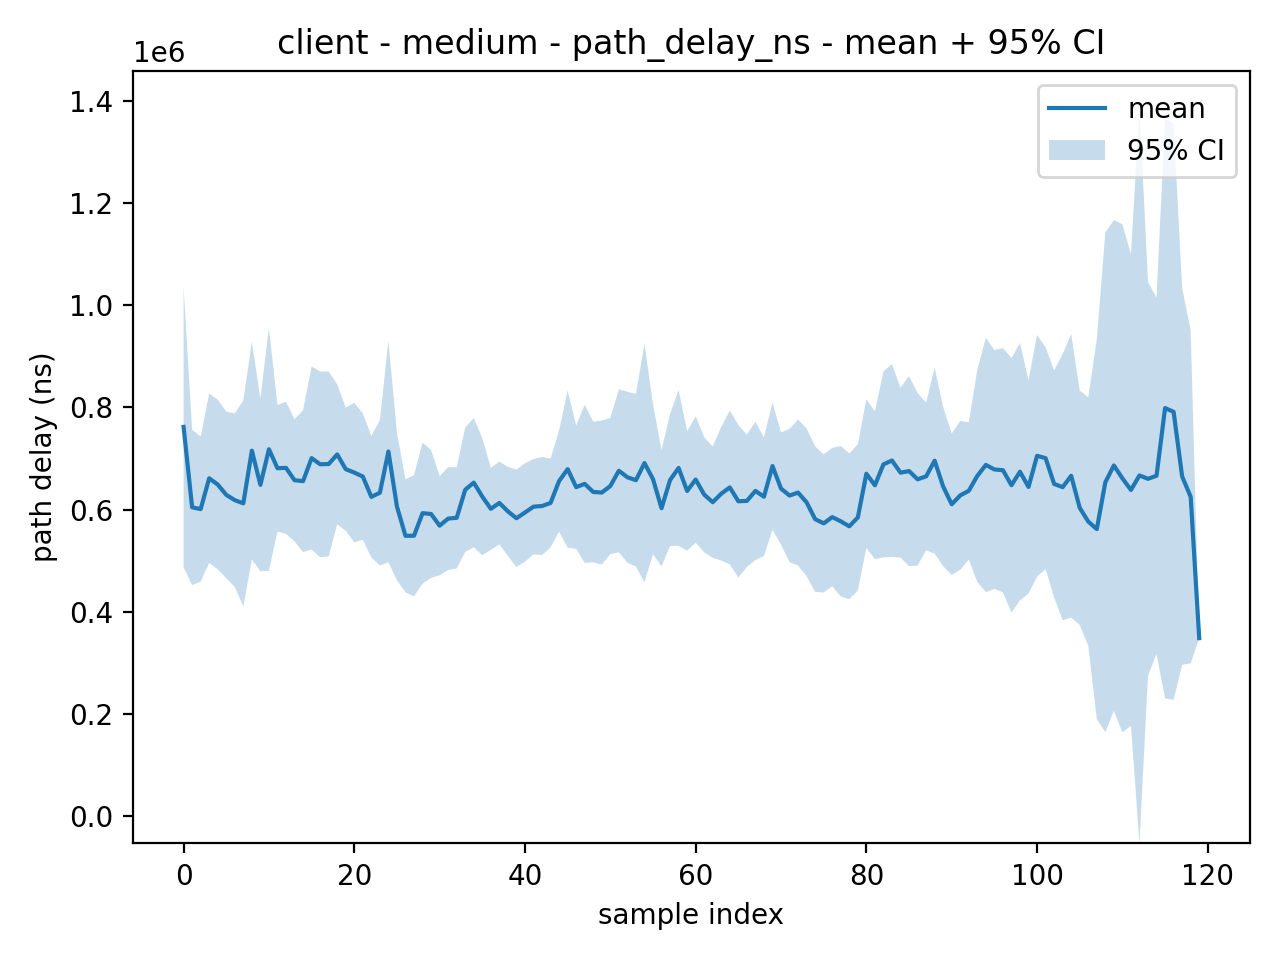
\includegraphics[width=\linewidth]{
      pars_plots/ptp/_aggregated/client/medium/path_delay_ns_mean_ci95.png
    }
    \caption{Scenario MEDIUM}
  \end{subfigure}
  \caption{Media con intervallo di confidenza al 95\% - nodo: \texttt{clientptp}}
  \label{fig:scenario_comparison}
\end{figure}
\begin{figure}[H]
  \centering

  \begin{subfigure}
    {0.4\textwidth}
    \centering
    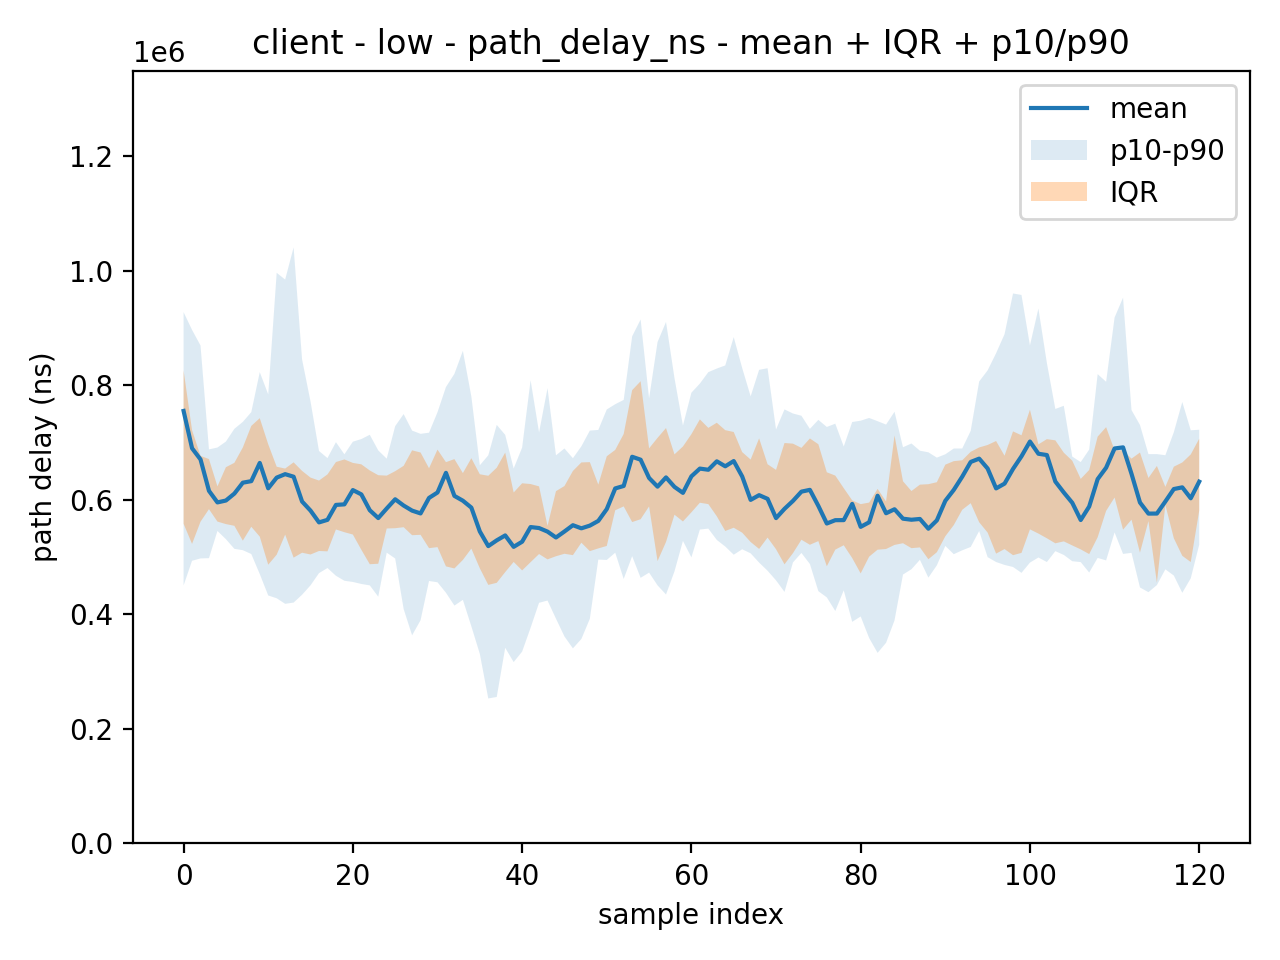
\includegraphics[width=\linewidth]{
      pars_plots/ptp/_aggregated/client/low/path_delay_ns_mean_iqr_p10_p90.png
    }
    \caption{Scenario LOW}
  \end{subfigure}
  \hfill
  \begin{subfigure}
    {0.4\textwidth}
    \centering
    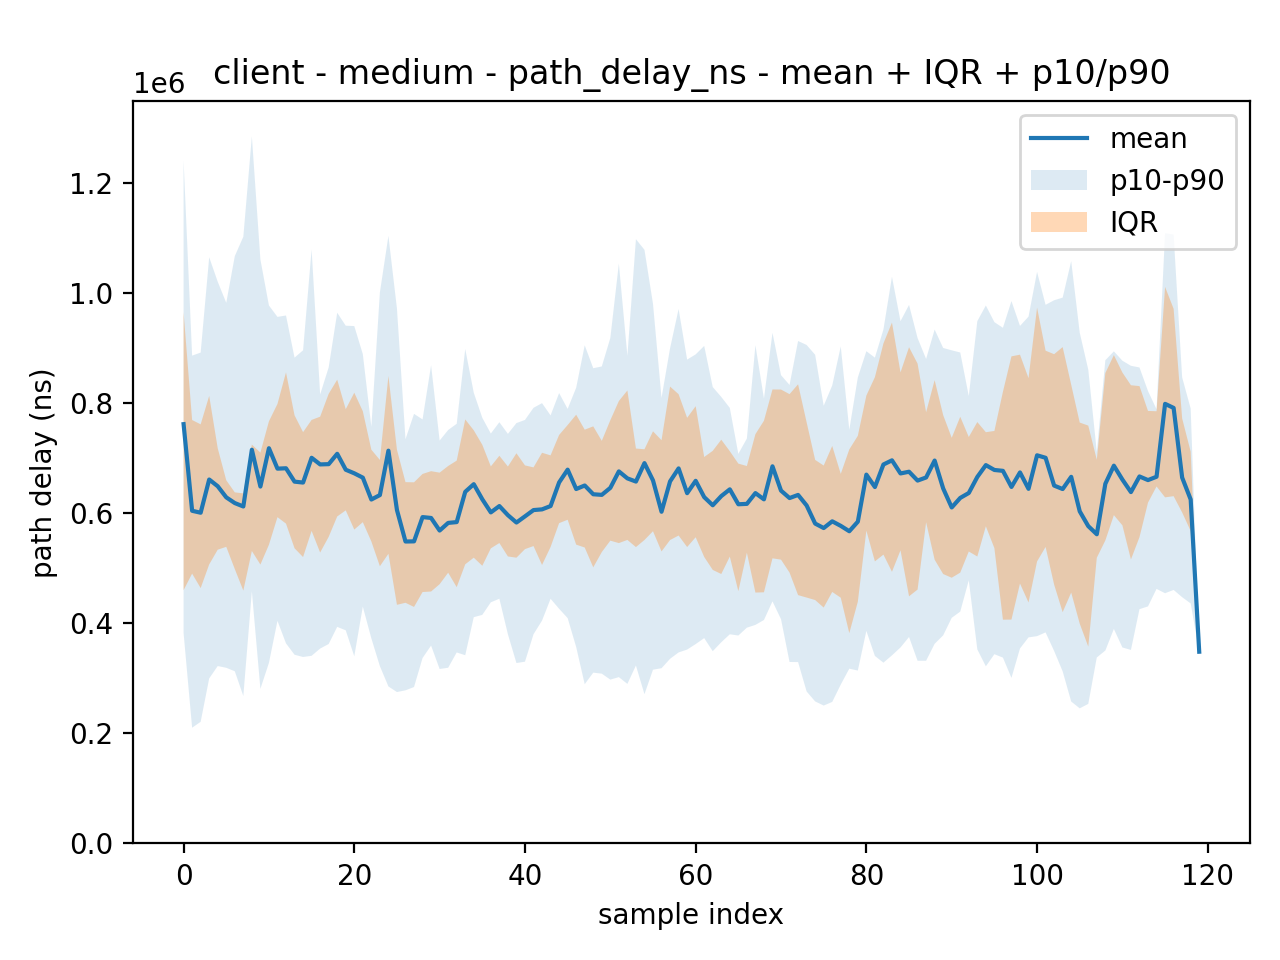
\includegraphics[width=\linewidth]{
      pars_plots/ptp/_aggregated/client/medium/path_delay_ns_mean_iqr_p10_p90.png
    }
    \caption{Scenario MEDIUM}
  \end{subfigure}
  \caption{Media con banda interquartile e banda p10-p90 - nodo: \texttt{clientptp}}
  \label{fig:scenario_comparison}
\end{figure}

La metrica \texttt{path delay} sul nodo \texttt{clientptp} consente di valutare
il ritardo stimato lungo il percorso di sincronizzazione tra il client e il
master. Nel caso del demone PTP, l’analisi quantitativa di tale grandezza può
essere condotta soltanto sugli scenari \texttt{low} e \texttt{medium}, poiché nello
scenario \texttt{high} non viene raggiunta una condizione sufficientemente
stabile da produrre una serie di campioni confrontabile con le altre due
condizioni sperimentali.

Nel caso \texttt{low}, il \texttt{path delay} presenta un andamento mediamente regolare
e si colloca su valori dell’ordine di alcune centinaia di microsecondi. La curva
aggregata assume un valore medio pari a circa $606.8\,\mu s$, con mediana pari a circa
$602.5\,\mu s$. La distribuzione dei valori centrali della serie si concentra in
una fascia relativamente contenuta, con intervallo interquartile compreso approssimativamente
tra $575.8\,\mu s$ e $638.6\,\mu s$. Anche dal punto di vista grafico
l’andamento risulta abbastanza stabile, pur con oscillazioni locali non trascurabili,
ma complessivamente compatibili con una condizione di rete moderatamente
controllata.

Nel caso \texttt{medium}, il livello medio del \texttt{path delay} cresce, ma in
misura contenuta. La curva aggregata assume infatti un valore medio pari a circa $6
42.2\,\mu s$, con mediana pari a circa $645.5\,\mu s$. L’incremento rispetto allo
scenario \texttt{low} è dunque dell’ordine di alcune decine di microsecondi, e non
evidenzia una discontinuità marcata nel livello della metrica. Tuttavia, lo scenario
\texttt{medium} mostra una dispersione più elevata: l’intervallo interquartile della
curva centrale si colloca approssimativamente tra $613.0\,\mu s$ e $672.3\,\mu s$,
mentre le bande di variabilità rappresentate nei grafici risultano mediamente
più ampie rispetto al caso \texttt{low}. In particolare, aumentano sia l’ampiezza
dell’IQR sia quella della fascia $p10$--$p90$, segnalando una minore regolarità della
stima del ritardo di percorso.

Nel complesso, il confronto tra \texttt{low} e \texttt{medium} mostra che, per il
nodo \texttt{clientptp}, il degrado della rete non produce un forte aumento del valore
medio del \texttt{path delay}, ma si riflette soprattutto in una maggiore variabilità
delle misurazioni. La metrica risulta quindi sensibile al peggioramento dello
scenario sperimentale, ma l’effetto osservato si manifesta principalmente come perdita
di stabilità più che come incremento netto del livello centrale. Per lo scenario
\texttt{high}, come già discusso, non è invece possibile formulare un confronto quantitativo,
poiché il client non raggiunge una condizione operativa stabile tale da generare
una serie di campioni omogenea e utilizzabile ai fini statistici, rafforzando un evidenza
del degrado indotto dovuto a elevati parametri di congestione di rete.

\subsubsection{Analisi metrica: \texttt{RMS offset}}
\begin{figure}[H]
  \centering

  \begin{subfigure}
    {0.4\textwidth}
    \centering
    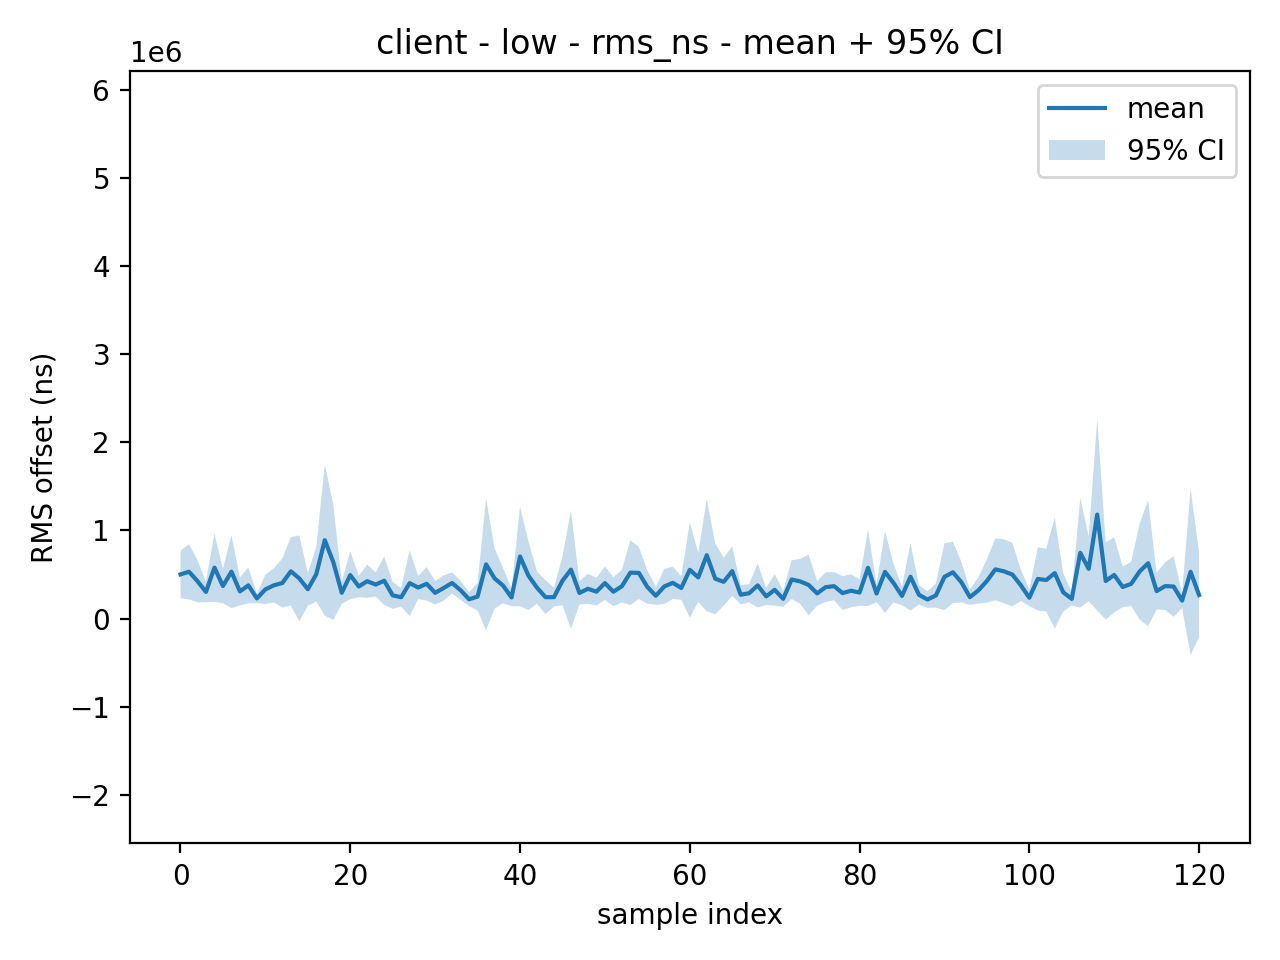
\includegraphics[width=\linewidth]{
      pars_plots/ptp/_aggregated/client/low/rms_ns_mean_ci95.png
    }
    \caption{Scenario LOW}
  \end{subfigure}
  \hfill
  \begin{subfigure}
    {0.4\textwidth}
    \centering
    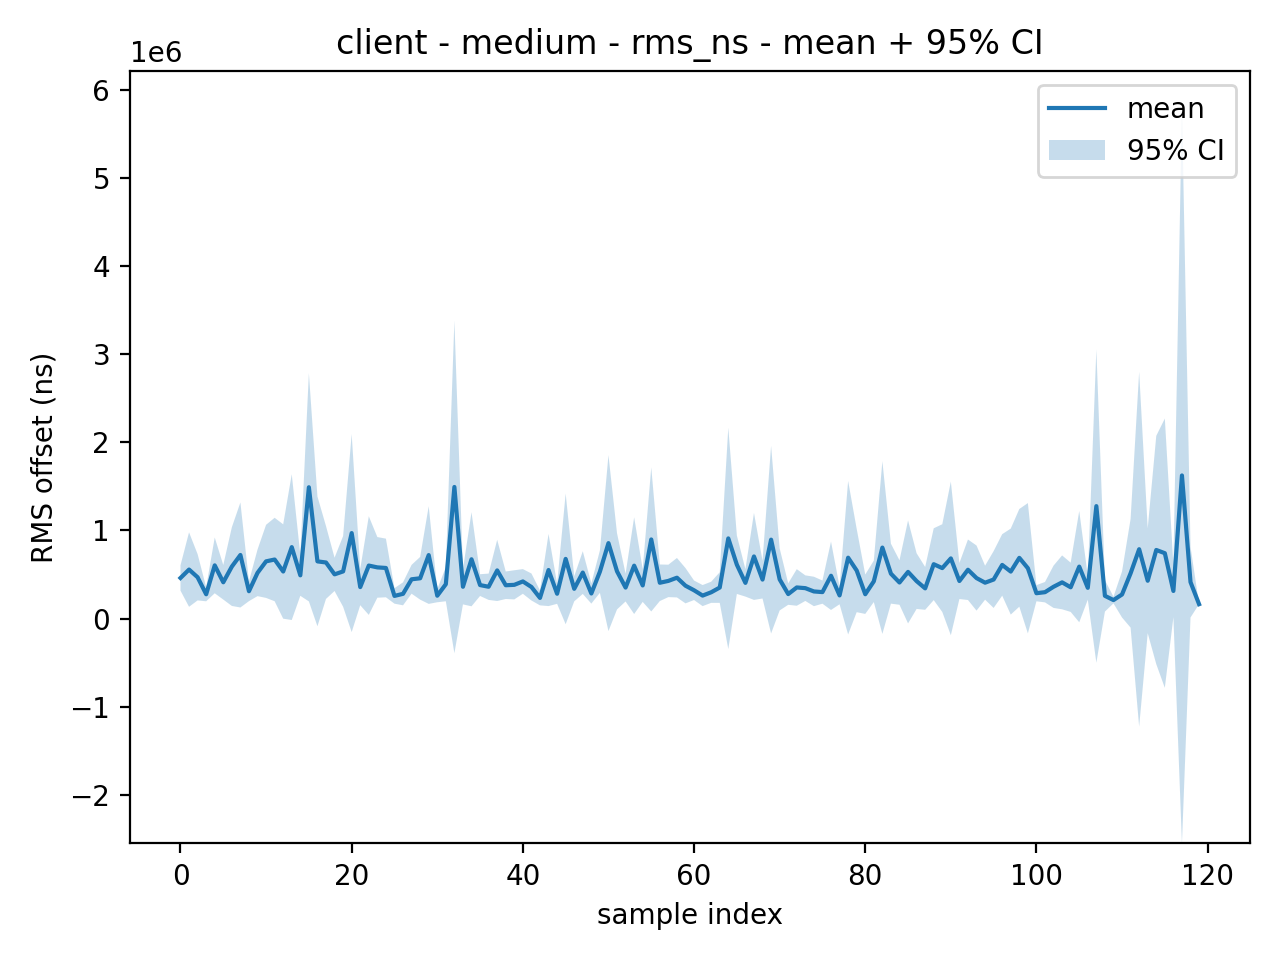
\includegraphics[width=\linewidth]{
      pars_plots/ptp/_aggregated/client/medium/rms_ns_mean_ci95.png
    }
    \caption{Scenario MEDIUM}
  \end{subfigure}
  \caption{Media con intervallo di confidenza al 95\% - nodo: \texttt{clientptp}}
  \label{fig:scenario_comparison}
\end{figure}
\begin{figure}[H]
  \centering

  \begin{subfigure}
    {0.4\textwidth}
    \centering
    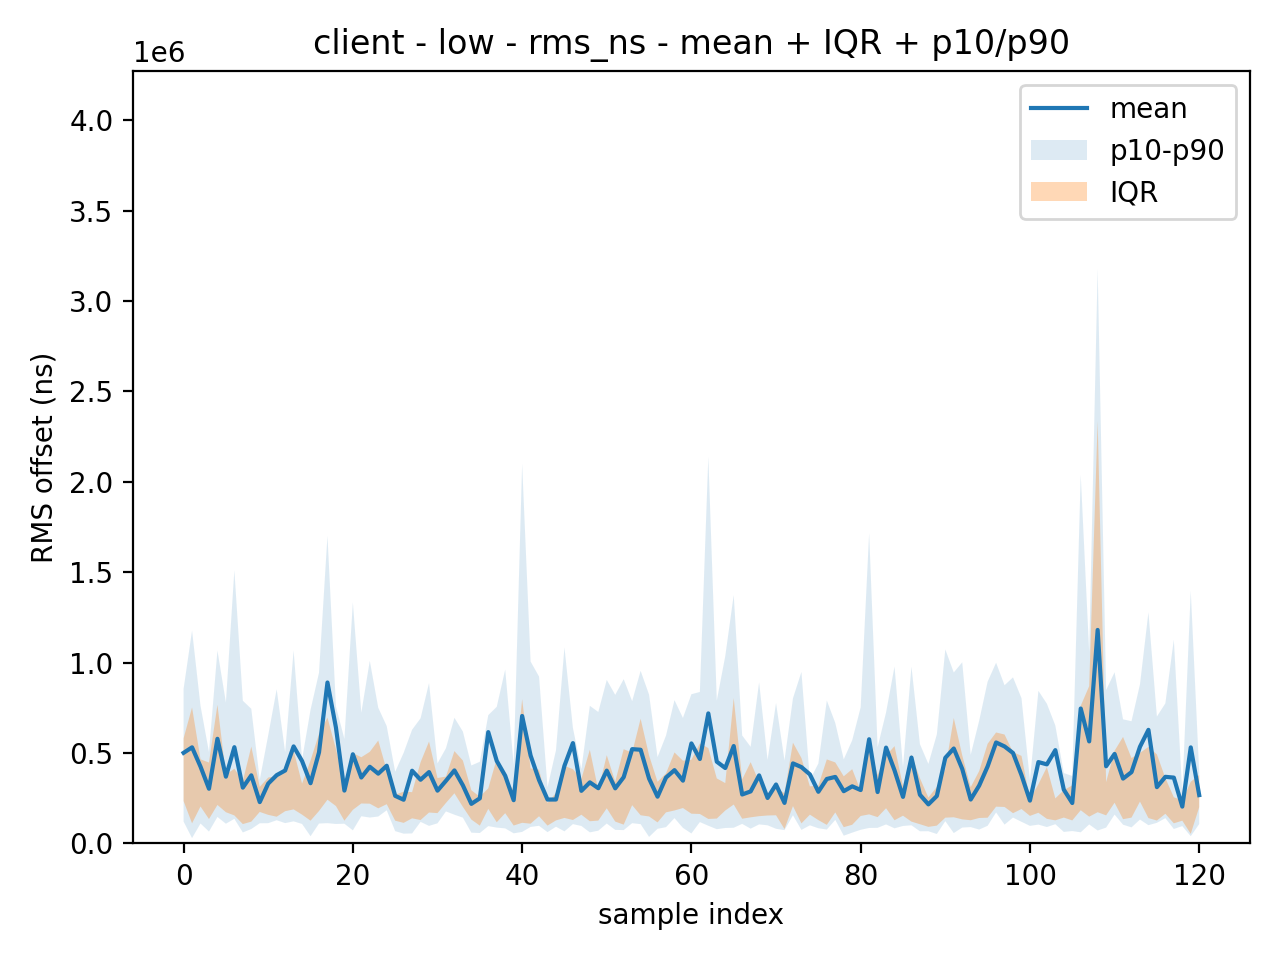
\includegraphics[width=\linewidth]{
      pars_plots/ptp/_aggregated/client/low/rms_ns_mean_iqr_p10_p90.png
    }
    \caption{Scenario LOW}
  \end{subfigure}
  \hfill
  \begin{subfigure}
    {0.4\textwidth}
    \centering
    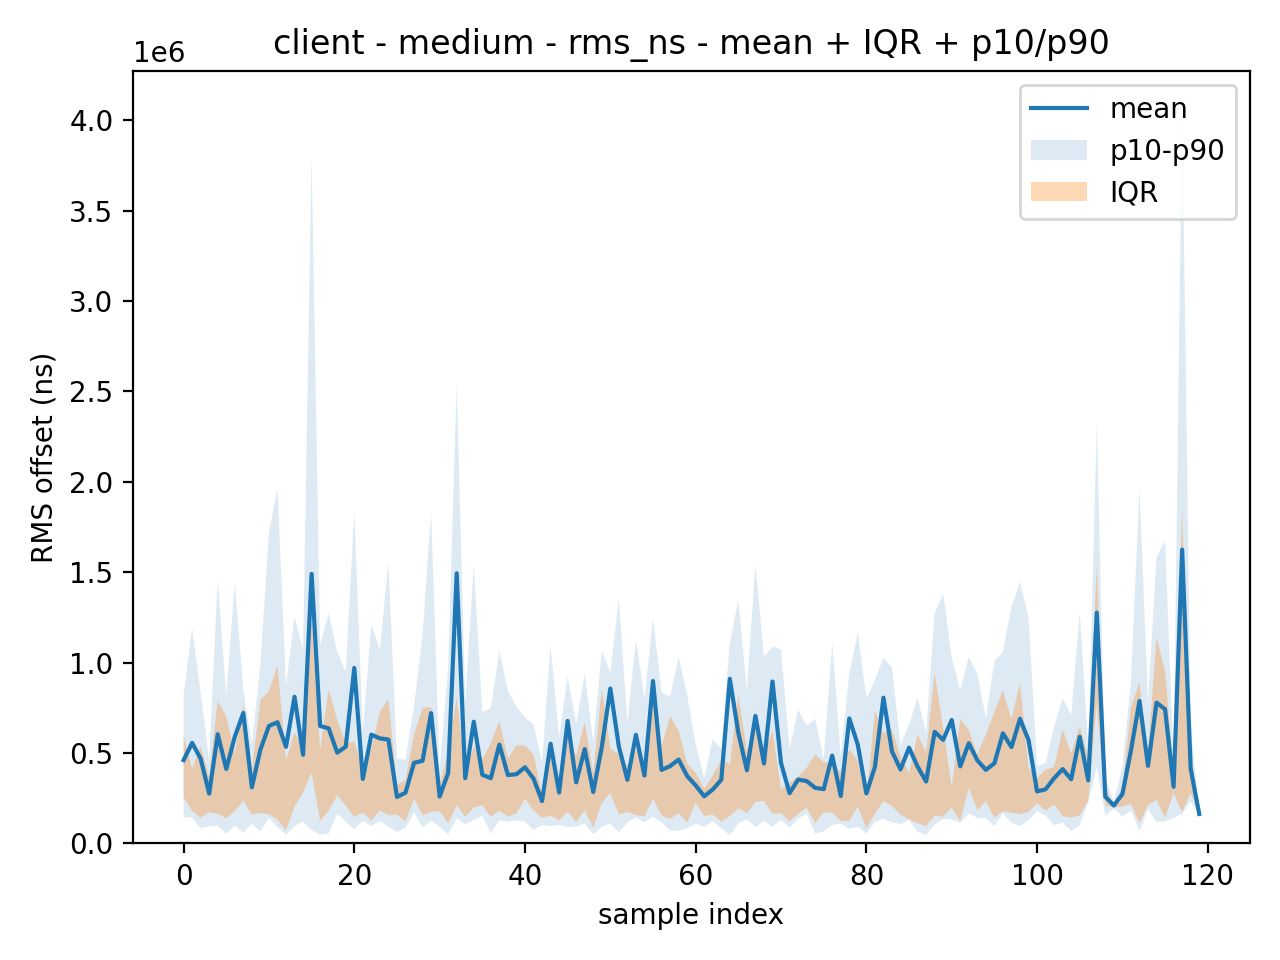
\includegraphics[width=\linewidth]{
      pars_plots/ptp/_aggregated/client/medium/rms_ns_mean_iqr_p10_p90.png
    }
    \caption{Scenario MEDIUM}
  \end{subfigure}
  \caption{Media con banda interquartile e banda p10-p90 - nodo: \texttt{clientptp}}
  \label{fig:scenario_comparison}
\end{figure}

La metrica \texttt{RMS} sul nodo \texttt{clientptp} sintetizza l’entità media
dell’errore di sincronizzazione osservato dal client PTP e fornisce quindi una
misura complessiva della qualità temporale raggiunta dal nodo nel corso
dell’esperimento. Anche in questo caso, il confronto quantitativo può essere
sviluppato soltanto sugli scenari \texttt{low} e \texttt{medium}, poiché nello scenario
\texttt{high} il client non raggiunge una condizione operativa stabile tale da
generare una serie numerica confrontabile.

Nel caso \texttt{low}, la metrica RMS si mantiene su valori medi dell’ordine di
alcune centinaia di microsecondi. La curva aggregata presenta infatti un valore medio
pari a circa $406.7\,\mu s$, con mediana pari a circa $378.1\,\mu s$. La distribuzione
dei valori centrali si colloca prevalentemente in una fascia compresa tra circa $3
02.5\,\mu s$ e $493.2\,\mu s$, pur in presenza di alcuni picchi locali più
elevati. L’andamento della serie risulta nel complesso irregolare ma ancora contenuto
entro limiti compatibili con una condizione di rete relativamente favorevole.

Nel caso \texttt{medium}, la RMS aumenta in modo più evidente rispetto a quanto osservato
per la metrica di \texttt{path delay}. Il valore medio della curva aggregata sale
infatti a circa $514.9\,\mu s$, mentre la mediana si attesta intorno a
$458.5\,\mu s$. Rispetto allo scenario \texttt{low}, si osserva quindi un incremento
sensibile del livello della metrica, pari a poco più di $100\,\mu s$. Tuttavia,
l’aspetto più rilevante è rappresentato dall’aumento della dispersione: l’intervallo
interquartile dei valori centrali si amplia, le bande di variabilità nei grafici
risultano più estese e la serie mostra una maggiore presenza di spike e
oscillazioni ampie. In particolare, aumentano sia l’ampiezza dell’IQR sia quella
della fascia $p10$--$p90$, indicando una minore stabilità della sincronizzazione.

Nel complesso, la metrica RMS evidenzia in modo chiaro il peggioramento del comportamento
del nodo \texttt{clientptp} nel passaggio da \texttt{low} a \texttt{medium}. A differenza
di quanto osservato sul \texttt{path delay}, in questo caso il degrado non si manifesta
soltanto come aumento della variabilità, ma anche come incremento apprezzabile
del livello medio dell’errore temporale. La RMS risulta dunque una metrica particolarmente
utile per mettere in evidenza la perdita di qualità della sincronizzazione PTP al
crescere della severità dello scenario di rete. Per lo scenario \texttt{high},
come già osservato, non è invece possibile sviluppare un confronto quantitativo,
poiché il client non raggiunge una condizione di sincronizzazione stabile, confermando
l'eccessivo degrado di rete che non permette a \texttt{clientptp} di
stabilizarsi.

\subsection{\texttt{boundary}}
L'analisi relativa al nodo \texttt{boundary} deve essere interpretata in modo differente
rispetto a quella condotta sul client. Le metriche osservate in questo caso
descrivono infatti il comportamento della sincronizzazione del boundary rispetto
al \texttt{master upstream} (\texttt{servergm}), e non il collegamento downstream
verso il \texttt{clientptp}, sul quale è stato introdotto il degrado di rete. Di
conseguenza, in linea teorica, non ci si attende un impatto diretto e
strutturale degli impairment applicati nei tre scenari sulle misure di \texttt{offset}
e \texttt{path delay} rilevate sul boundary.

Occorre tuttavia considerare che il demone \texttt{ptp4l} opera sul nodo in modo unitario,
gestendo contemporaneamente più porte della topologia. Per tale ragione,
eventuali fault, transizioni di stato o condizioni di instabilità osservate sulla
porta downstream possono comunque riflettersi indirettamente sulla stabilità complessiva
del processo di sincronizzazione, introducendo fluttuazioni o anomalie anche
nelle metriche riferite al tratto upstream. L'analisi che segue è pertanto finalizzata
a verificare se i dati confermino una sostanziale stabilità del nodo \texttt{boundary}
nei tre scenari sperimentali, oppure se emergano effetti indiretti riconducibili alle
criticità operative osservate durante il testing.

\subsubsection{Analisi metrica: \texttt{path delay}}
\begin{figure}[H]
  \centering

  \begin{subfigure}
    {0.32\textwidth}
    \centering
    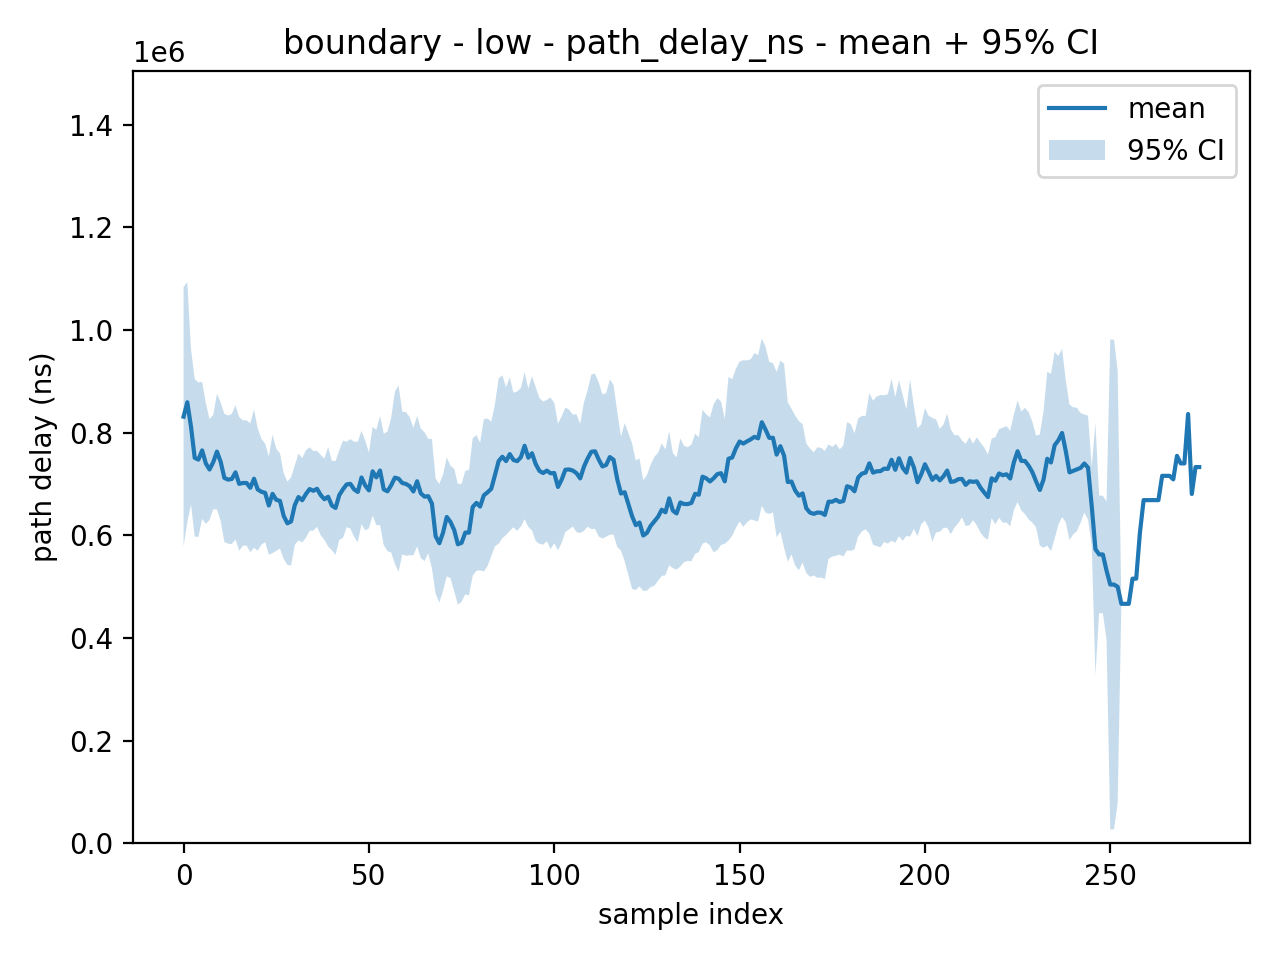
\includegraphics[width=\linewidth]{
      pars_plots/ptp/_aggregated/boundary/low/path_delay_ns_mean_ci95.png
    }
    \caption{Scenario LOW}
  \end{subfigure}
  \hfill
  \begin{subfigure}
    {0.32\textwidth}
    \centering
    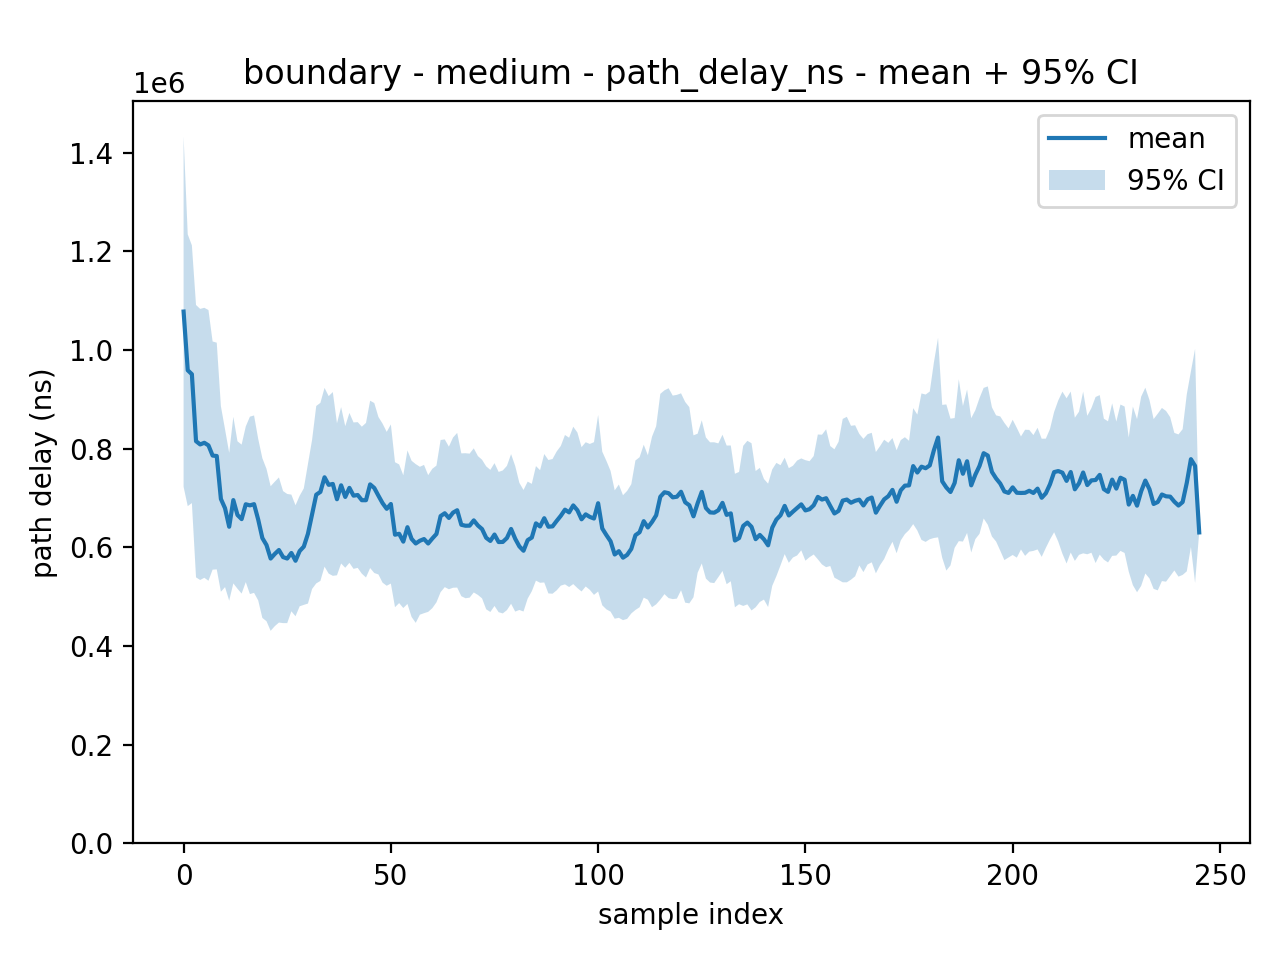
\includegraphics[width=\linewidth]{
      pars_plots/ptp/_aggregated/boundary/medium/path_delay_ns_mean_ci95.png
    }
    \caption{Scenario MEDIUM}
  \end{subfigure}
  \begin{subfigure}
    {0.32\textwidth}
    \centering
    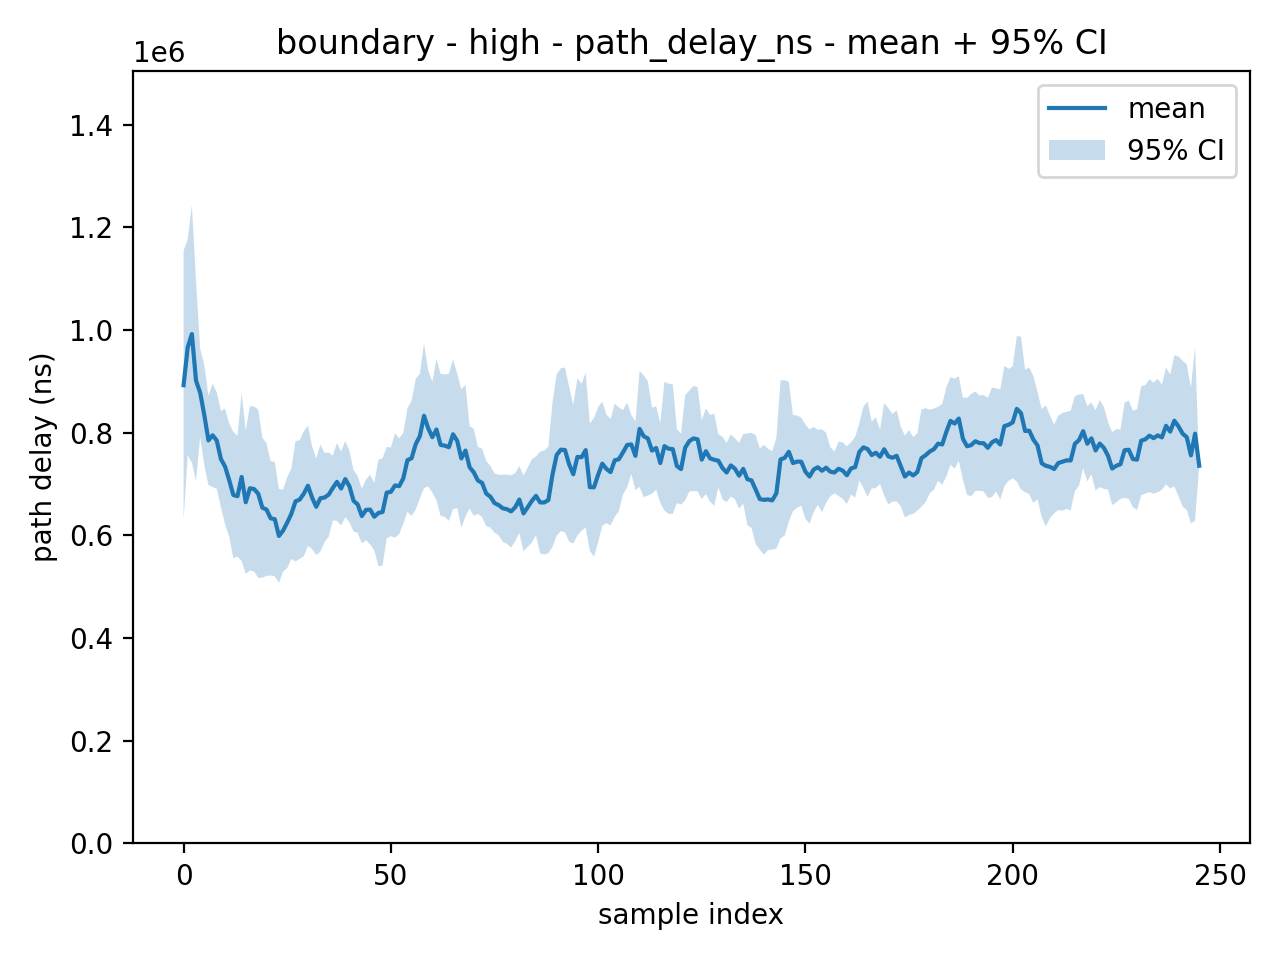
\includegraphics[width=\linewidth]{
      pars_plots/ptp/_aggregated/boundary/high/path_delay_ns_mean_ci95.png
    }
    \caption{Scenario HIGH}
  \end{subfigure}
  \caption{Media con intervallo di confidenza al 95\% - nodo: \texttt{boundary}}
  \label{fig:scenario_comparison}
\end{figure}
\begin{figure}[H]
  \centering

  \begin{subfigure}
    {0.32\textwidth}
    \centering
    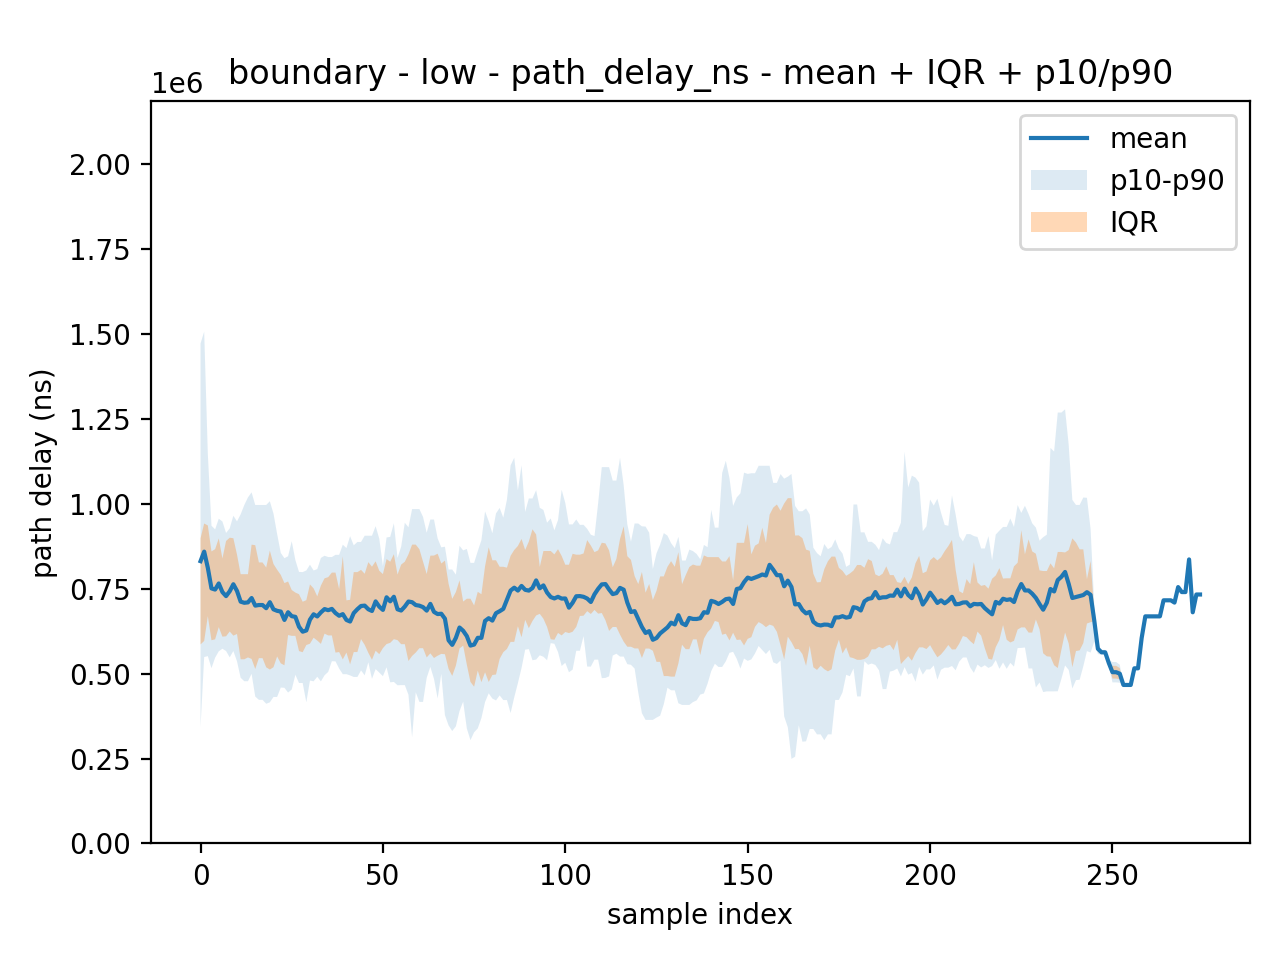
\includegraphics[width=\linewidth]{
      pars_plots/ptp/_aggregated/boundary/low/path_delay_ns_mean_iqr_p10_p90.png
    }
    \caption{Scenario LOW}
  \end{subfigure}
  \hfill
  \begin{subfigure}
    {0.32\textwidth}
    \centering
    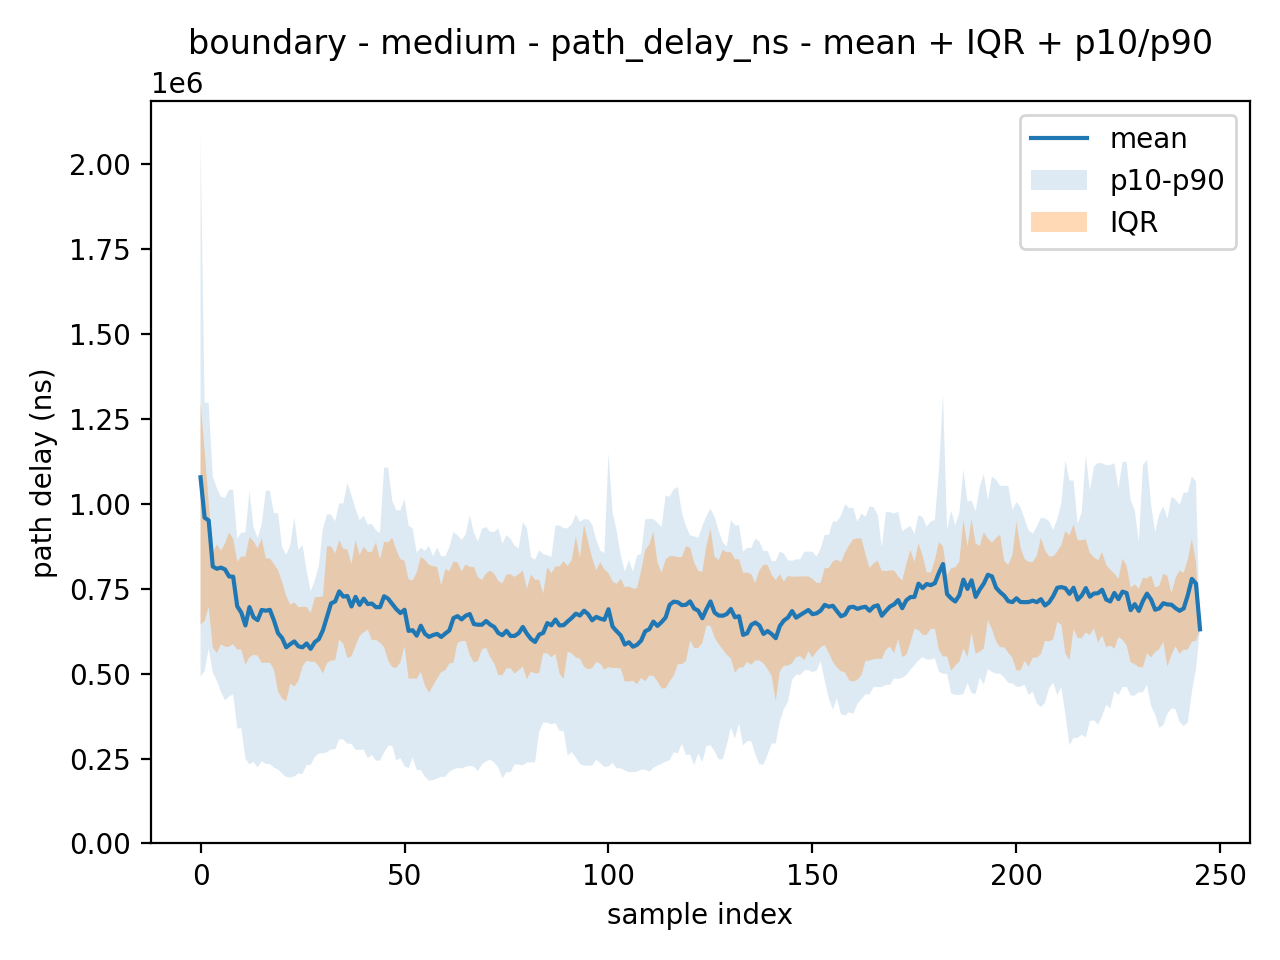
\includegraphics[width=\linewidth]{
      pars_plots/ptp/_aggregated/boundary/medium/path_delay_ns_mean_iqr_p10_p90.png
    }
    \caption{Scenario MEDIUM}
  \end{subfigure}
  \begin{subfigure}
    {0.32\textwidth}
    \centering
    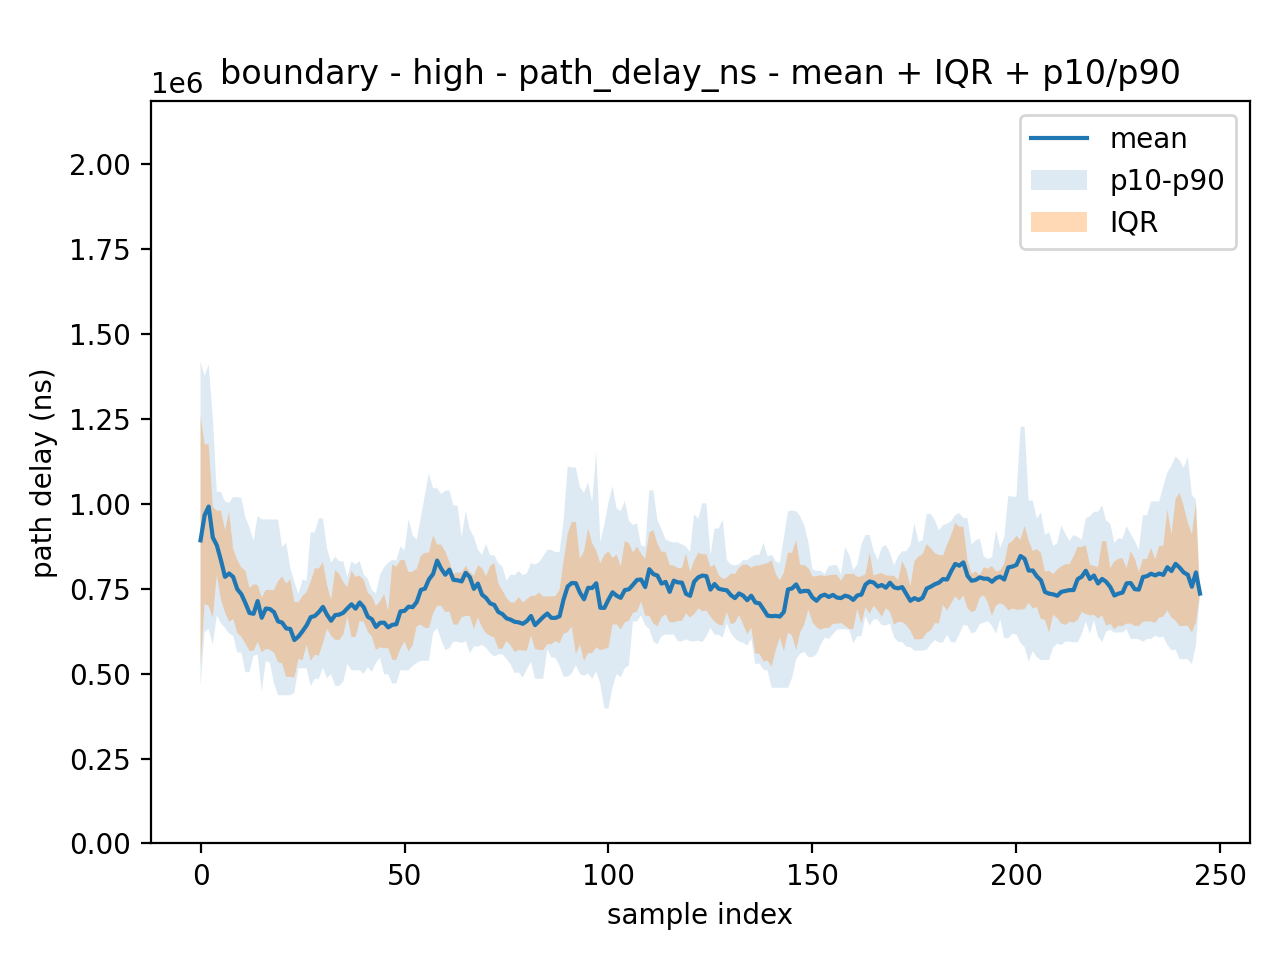
\includegraphics[width=\linewidth]{
      pars_plots/ptp/_aggregated/boundary/high/path_delay_ns_mean_iqr_p10_p90.png
    }
    \caption{Scenario HIGH}
  \end{subfigure}
  \caption{Media con banda interquartile e banda p10-p90 - nodo: \texttt{boundary}}
  \label{fig:scenario_comparison}
\end{figure}
L'analisi del \texttt{path delay} misurato sul nodo \texttt{boundary} conferma,
nel complesso, l'ipotesi di una sostanziale stabilità del collegamento verso il master
upstream anche al variare dello scenario di degrado applicato sul ramo downstream.
Le tre condizioni sperimentali presentano infatti valori medi dello stesso
ordine di grandezza e profili temporali complessivamente regolari, senza evidenza
di un deterioramento sistematico e monotono all'aumentare dell'impairment di rete.

Dal punto di vista quantitativo, il valore medio aggregato del \texttt{path
delay} risulta pari a circa 697.227~\textmu s nello scenario \texttt{low}, 687.669~\textmu
s nello scenario \texttt{medium} e 740.415~\textmu s nello scenario \texttt{high}.
Le differenze tra scenari sono quindi contenute e non indicano una variazione
strutturale del comportamento del boundary. Anche le misure di dispersione confermano
tale lettura: l'ampiezza interquartile media e la banda p10--p90 non mostrano infatti
un incremento progressivo e coerente con il livello di stress applicato,
evidenziando piuttosto oscillazioni moderate e non univocamente ordinate.

A livello grafico, nello scenario \texttt{low} la curva media oscilla attorno a
un livello pressoché stabile, con alcune fluttuazioni locali e una discontinuità più
marcata nella parte finale della serie. Lo scenario \texttt{medium} mostra un andamento
particolarmente regolare nel tratto centrale, mentre nello scenario \texttt{high}
si osserva un innalzamento moderato del livello medio, comunque compatibile con
una condizione di sincronizzazione ancora stabile. In nessun caso emerge un comportamento
riconducibile a una degradazione diretta del tratto upstream.

Nel complesso, i dati suggeriscono quindi che il \texttt{path delay} del \texttt{boundary}
resti sostanzialmente robusto rispetto agli impairment introdotti sul
collegamento downstream. Le variazioni osservate possono essere interpretate più plausibilmente
come effetti indiretti del funzionamento complessivo del demone \texttt{ptp4l}
sul nodo, piuttosto che come conseguenza diretta del degrado di rete imposto al client.

\subsubsection{Analisi metrica: \texttt{offset}}
\begin{figure}[H]
  \centering

  \begin{subfigure}
    {0.32\textwidth}
    \centering
    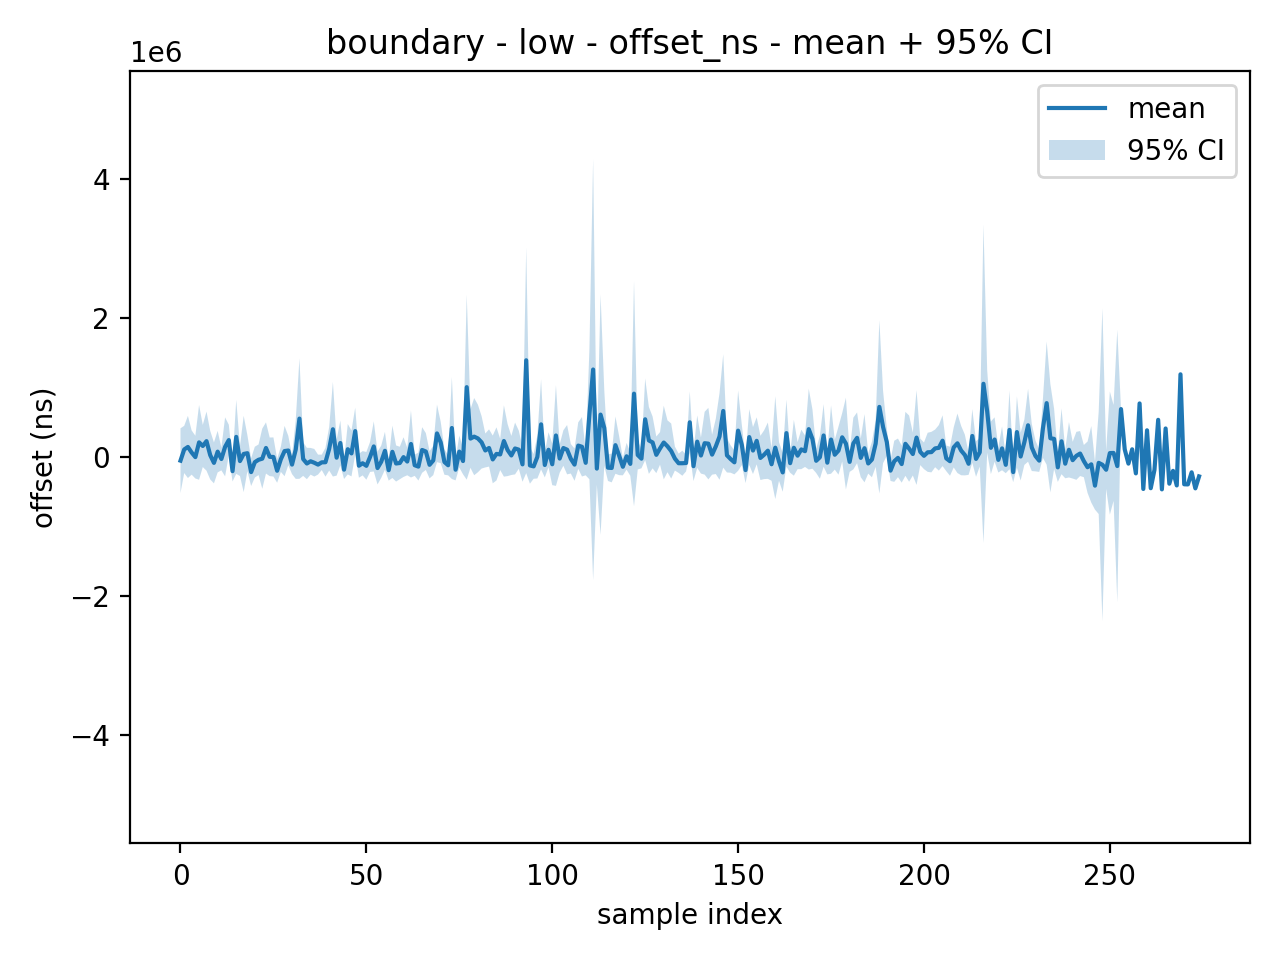
\includegraphics[width=\linewidth]{
      pars_plots/ptp/_aggregated/boundary/low/offset_ns_mean_ci95.png
    }
    \caption{Scenario LOW}
  \end{subfigure}
  \hfill
  \begin{subfigure}
    {0.32\textwidth}
    \centering
    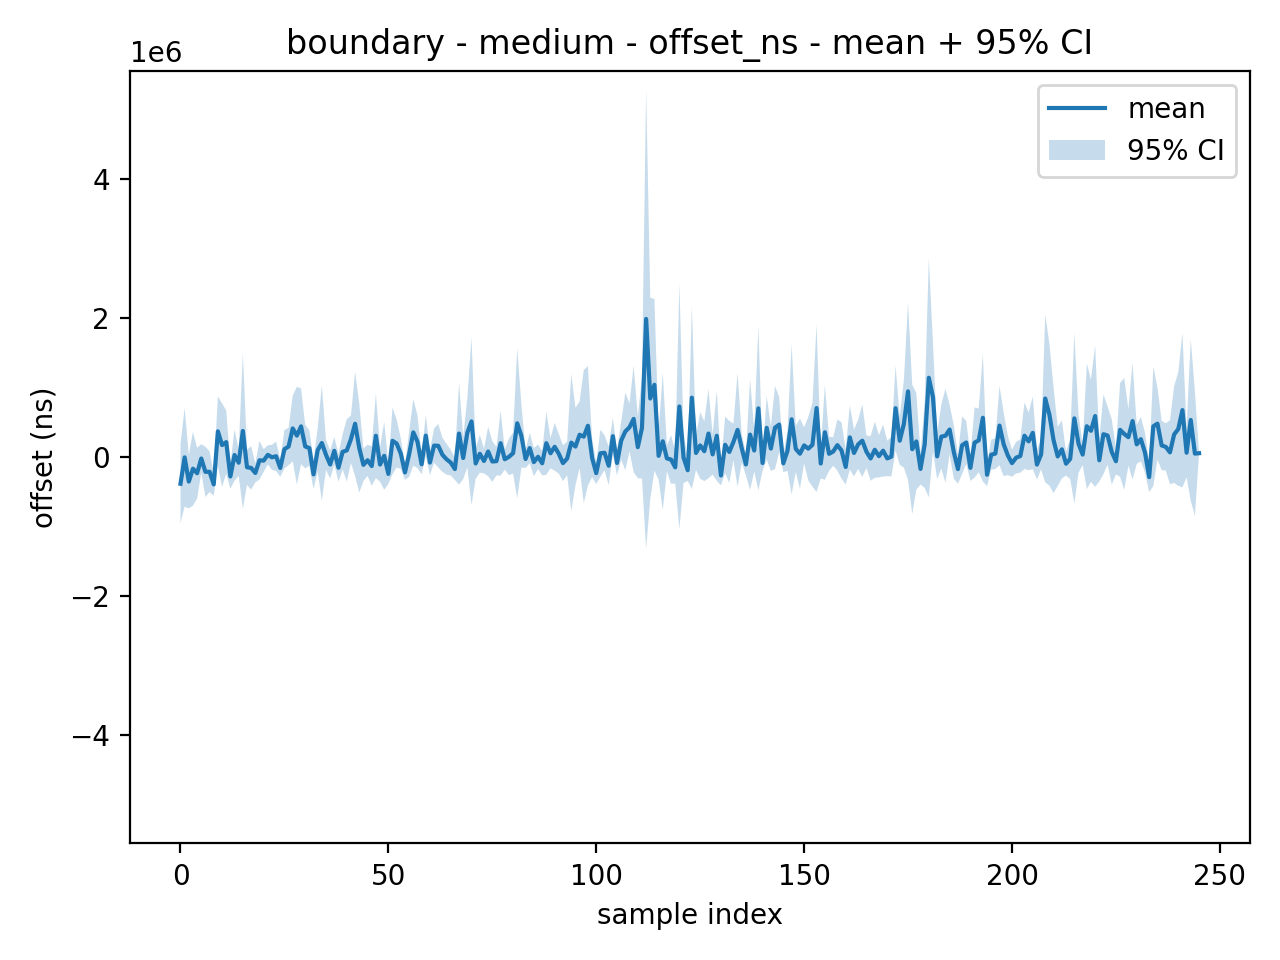
\includegraphics[width=\linewidth]{
      pars_plots/ptp/_aggregated/boundary/medium/offset_ns_mean_ci95.png
    }
    \caption{Scenario MEDIUM}
  \end{subfigure}
  \begin{subfigure}
    {0.32\textwidth}
    \centering
    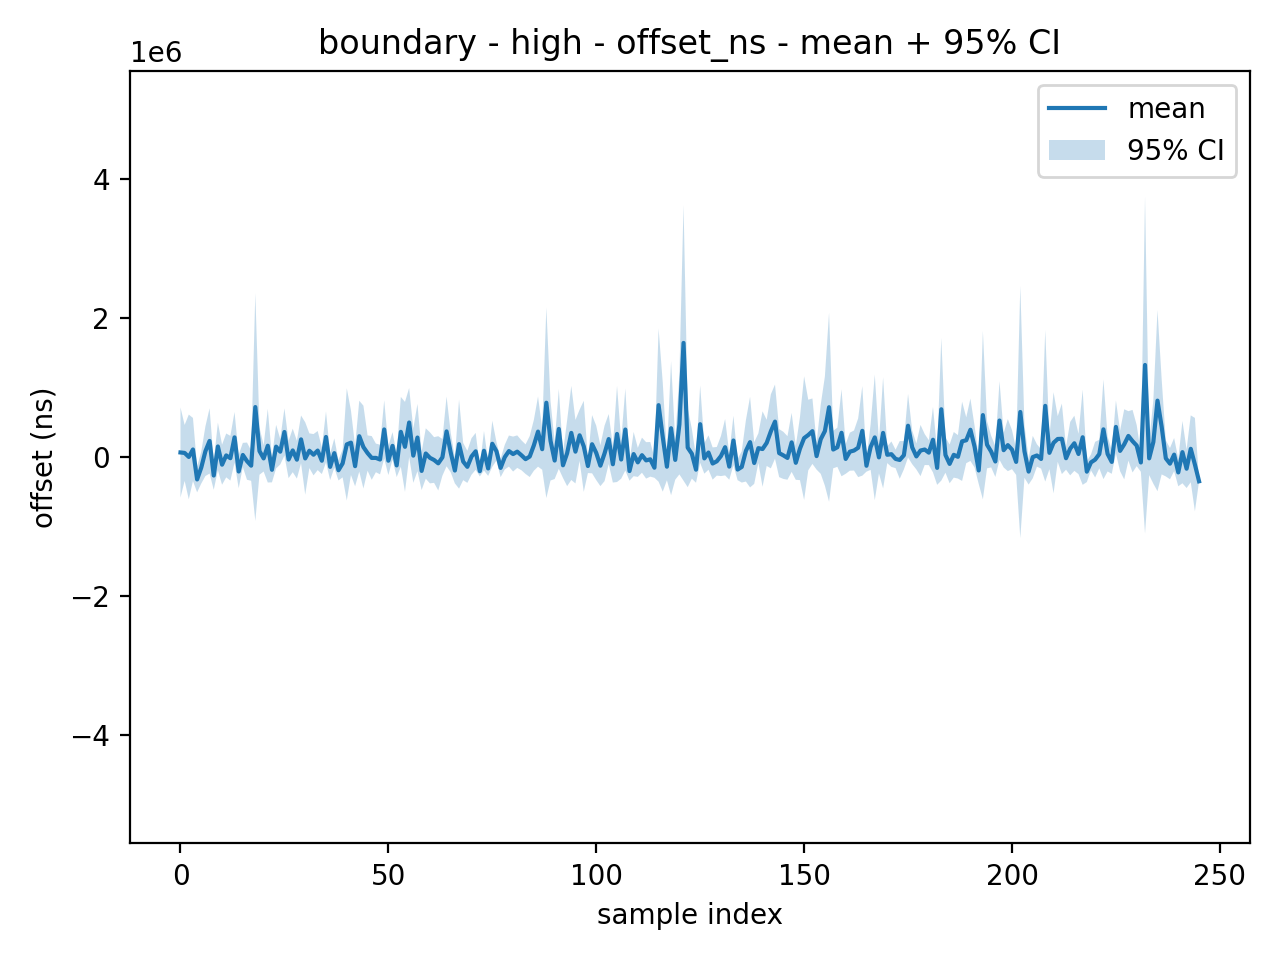
\includegraphics[width=\linewidth]{
      pars_plots/ptp/_aggregated/boundary/high/offset_ns_mean_ci95.png
    }
    \caption{Scenario HIGH}
  \end{subfigure}
  \caption{Media con intervallo di confidenza al 95\% - nodo: \texttt{boundary} -
  dati completi}
  \label{fig:scenario_comparison}
\end{figure}
\begin{figure}[H]
  \centering

  \begin{subfigure}
    {0.32\textwidth}
    \centering
    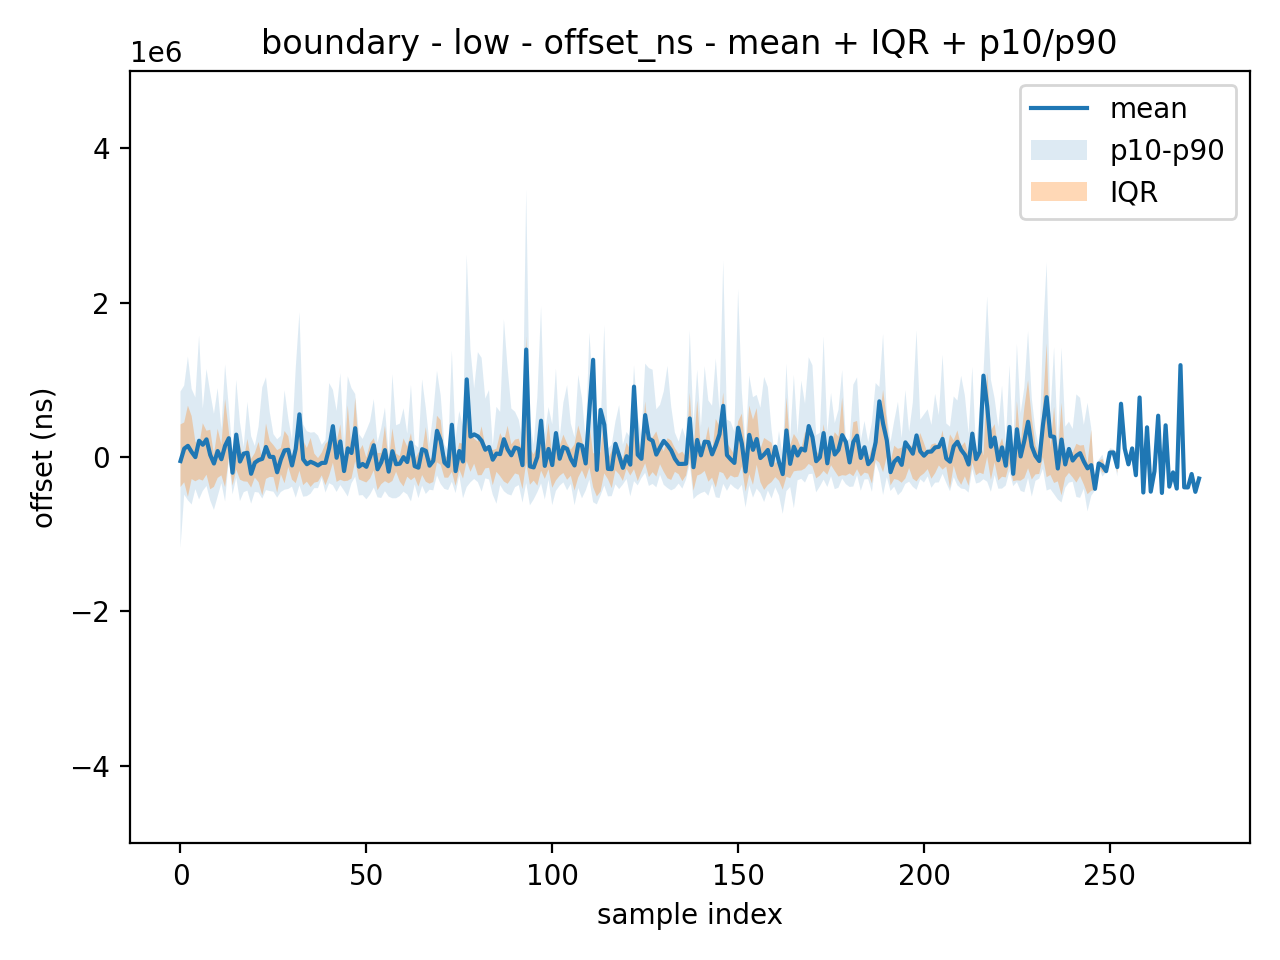
\includegraphics[width=\linewidth]{
      pars_plots/ptp/_aggregated/boundary/low/offset_ns_mean_iqr_p10_p90.png
    }
    \caption{Scenario LOW}
  \end{subfigure}
  \hfill
  \begin{subfigure}
    {0.32\textwidth}
    \centering
    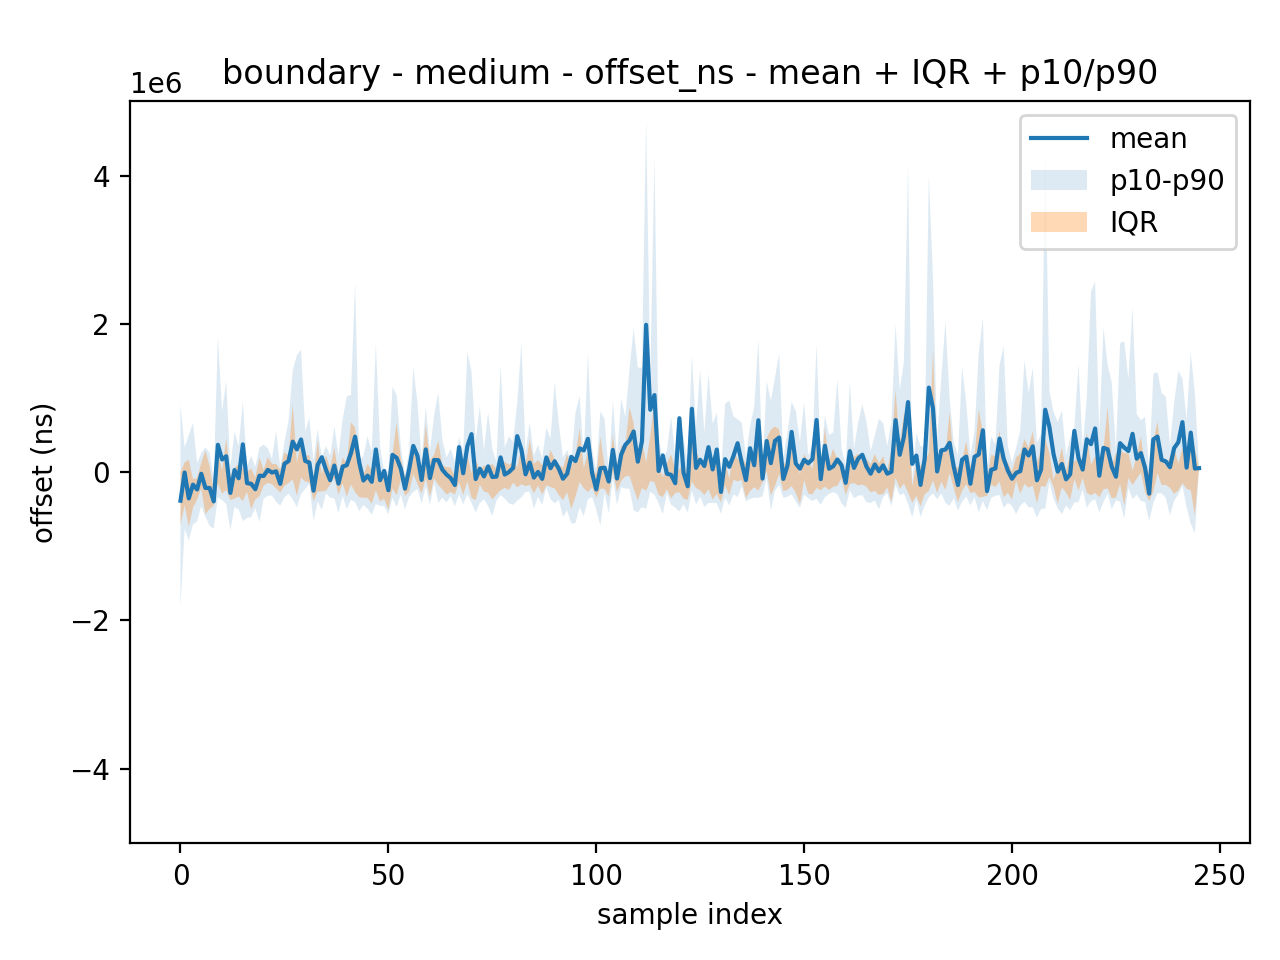
\includegraphics[width=\linewidth]{
      pars_plots/ptp/_aggregated/boundary/medium/offset_ns_mean_iqr_p10_p90.png
    }
    \caption{Scenario MEDIUM}
  \end{subfigure}
  \begin{subfigure}
    {0.32\textwidth}
    \centering
    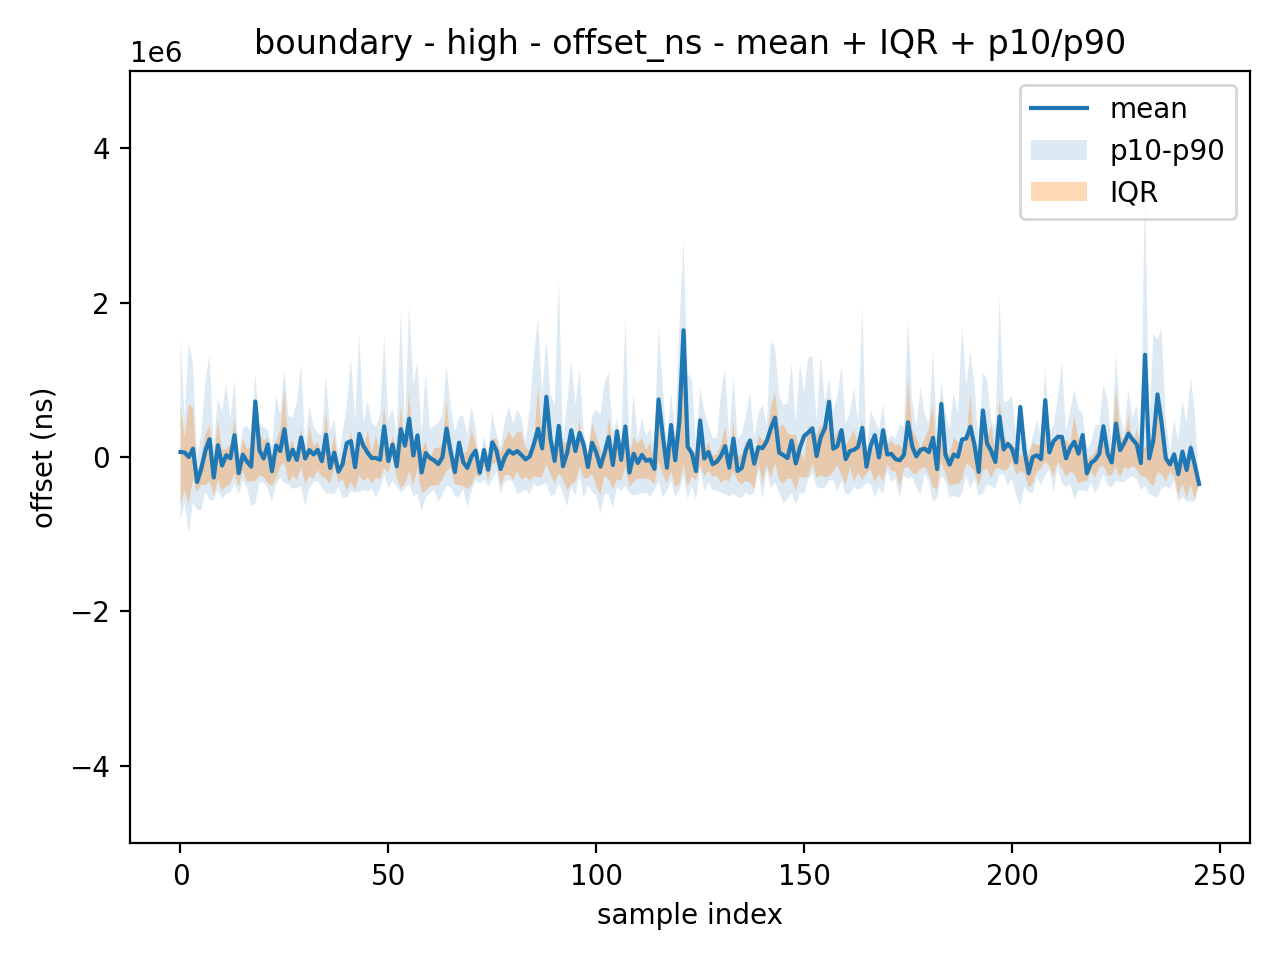
\includegraphics[width=\linewidth]{
      pars_plots/ptp/_aggregated/boundary/high/offset_ns_mean_iqr_p10_p90.png
    }
    \caption{Scenario HIGH}
  \end{subfigure}
  \caption{Media con banda interquartile e banda p10-p90 - nodo: \texttt{boundary}}
  \label{fig:scenario_comparison}
\end{figure}
L'analisi dell'\texttt{offset} misurato sul nodo \texttt{boundary} conferma,
anche in questo caso, l'assenza di un effetto diretto e sistematico degli impairment
applicati sul collegamento downstream verso il client. I tre scenari mostrano
infatti un andamento complessivamente centrato in prossimità dello zero, con oscillazioni
di segno alterno e picchi sporadici, ma senza una progressione monotona
riconducibile all'aumento del degrado di rete.

Dal punto di vista quantitativo, il valore medio aggregato dell'\texttt{offset}
risulta pari a circa 87.809~\textmu s nello scenario \texttt{low}, 153.961~\textmu
s nello scenario \texttt{medium} e 110.782~\textmu s nello scenario \texttt{high}.
Anche considerando la mediana, i valori restano contenuti e pari rispettivamente
a circa 45.375~\textmu s, 97.301~\textmu s e 65.087~\textmu s. Tali risultati
indicano quindi una lieve prevalenza di offset positivo, ma non una crescita strutturale
all'aumentare dello stress: lo scenario \texttt{medium} presenta il valore centrale
più elevato, mentre lo scenario \texttt{high} torna su livelli più contenuti e più
vicini a quelli del caso \texttt{low}.

Anche le misure di dispersione confermano questa interpretazione. L'ampiezza interquartile
media è pari a circa 279.114~\textmu s nello scenario \texttt{low}, 327.530~\textmu
s nello scenario \texttt{medium} e 250.843~\textmu s nello scenario \texttt{high};
analogamente, la banda p10--p90 media assume valori pari a circa 1017.673~\textmu
s, 1243.040~\textmu s e 1122.148~\textmu s. Anche in questo caso non si osserva
un incremento regolare e cumulativo della variabilità al crescere dell'impairment:
lo scenario \texttt{medium} appare il più disperso, mentre lo scenario \texttt{high}
non peggiora ulteriormente e mantiene una dispersione comparabile, se non in parte
inferiore, rispetto al caso intermedio.

L'osservazione dei profili temporali porta alle stesse conclusioni. Nel caso \texttt{low}
la serie è caratterizzata da oscillazioni contenute attorno allo zero, intervallate
da alcuni spike isolati di maggiore ampiezza e da una parte finale leggermente più
irregolare. Lo scenario \texttt{medium} mostra una dinamica molto simile, con
una maggiore frequenza di escursioni positive e una variabilità lievemente più
pronunciata in alcuni tratti centrali. Nel caso \texttt{high}, pur in presenza di
picchi locali anche rilevanti, la curva media rimane comunque prossima allo zero
e non evidenzia deriva persistente né instabilità sistematica.

Nel complesso, l'\texttt{offset} del \texttt{boundary} conferma quindi una condizione
di sostanziale stabilità della sincronizzazione sul tratto upstream. Le
differenze osservate tra i tre scenari appaiono limitate, non monotone e non sufficienti
a sostenere l'ipotesi di un impatto diretto del degrado downstream sulla sincronizzazione
del \texttt{boundary} rispetto al \texttt{servergm}. Gli eventuali scostamenti
locali sono più plausibilmente interpretabili come fluttuazioni operative del
processo \texttt{ptp4l} o come effetti indiretti transitori, piuttosto che come
conseguenza strutturale del livello di stress applicato al client.

\section{\texttt{chronyd}}
Nel caso di \texttt{Chrony}, l’analisi è stata svolta su una topologia composta
dal solo collegamento tra \texttt{servergm} e \texttt{clientchrony}, senza la presenza
di nodi \texttt{boundary}. In questo contesto, il degrado di rete tramite
\texttt{tc}/\texttt{netem} è stato applicato in due configurazioni distinte: in un
primo caso sull’interfaccia del \texttt{clientchrony}, in un secondo caso sull’interfaccia
del \texttt{servergm}.

Questa doppia configurazione consente di osservare separatamente gli effetti del
degrado introdotto lungo le due direzioni logiche della comunicazione tra client
e server. Poiché il meccanismo di sincronizzazione di \texttt{Chrony} si basa
sullo scambio di messaggi tra i due estremi, applicare l’alterazione su un lato oppure
sull’altro permette di valutare se il posizionamento del disturbo lungo il percorso
influenzi in modo differente le metriche osservate.

Nel seguito verranno quindi confrontati non solo i diversi livelli di stress di rete,
ma anche i risultati ottenuti nelle due configurazioni di applicazione del
degrado. È inoltre opportuno precisare che tutte le metriche analizzate sono state
rilevate esclusivamente tramite interrogazione del nodo \texttt{clientchrony}, poiché
è da esso che si ricavano le misure direttamente rilevanti per valutare la qualità
della sincronizzazione dal punto di vista del client.

\subsection{Analisi metrica: \texttt{offset}}
\begin{figure}[H]
  \centering

  \begin{subfigure}
    {0.32\textwidth}
    \centering
    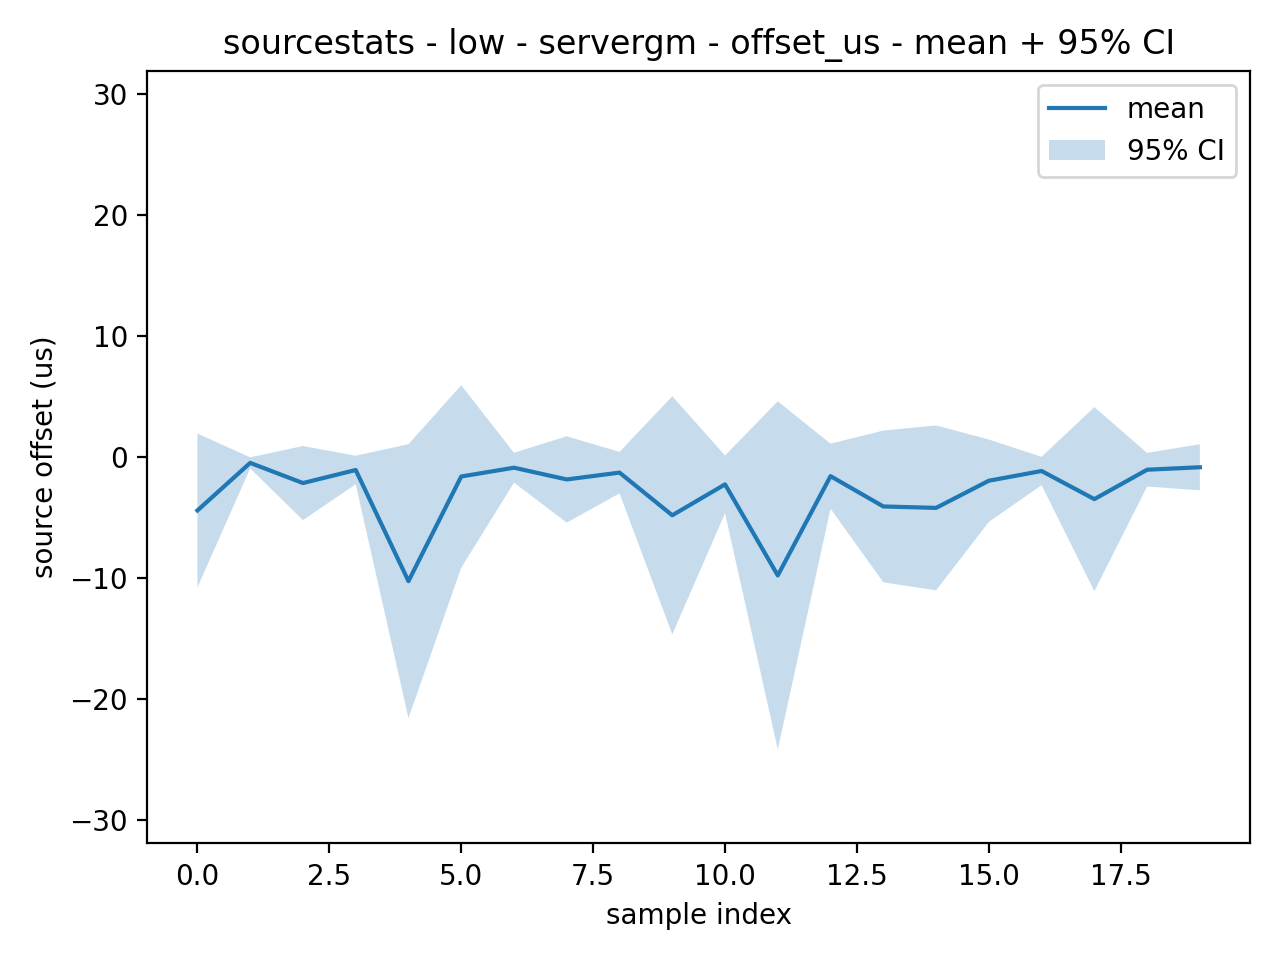
\includegraphics[width=\linewidth]{
      pars_plots/chrony_clientchrony/_aggregated/sourcestats/low/servergm/offset_us_mean_ci95.png
    }
    \caption{Scenario LOW}
  \end{subfigure}
  \hfill
  \begin{subfigure}
    {0.32\textwidth}
    \centering
    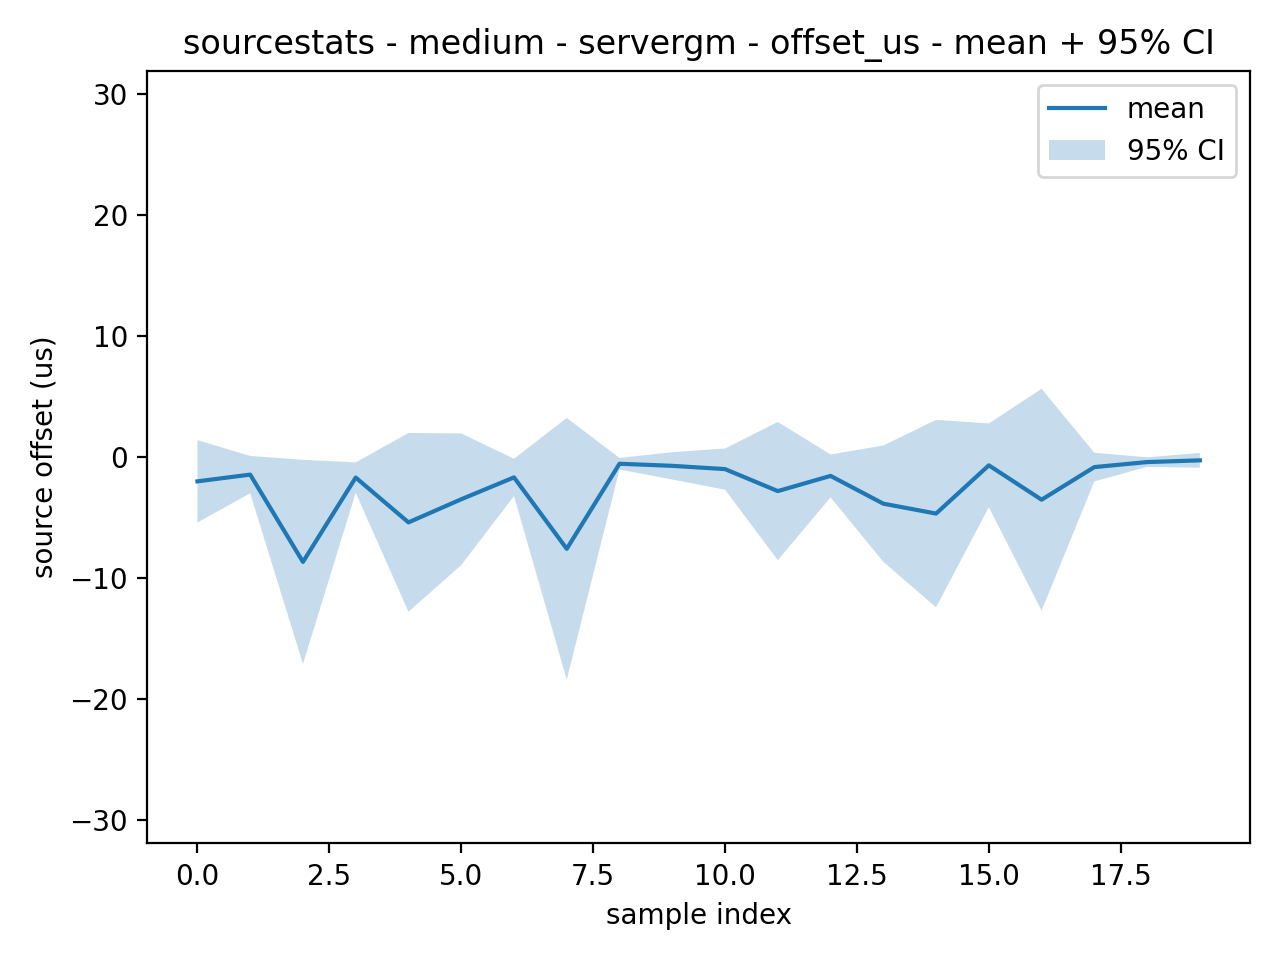
\includegraphics[width=\linewidth]{
      pars_plots/chrony_clientchrony/_aggregated/sourcestats/medium/servergm/offset_us_mean_ci95.png
    }
    \caption{Scenario MEDIUM}
  \end{subfigure}
  \begin{subfigure}
    {0.32\textwidth}
    \centering
    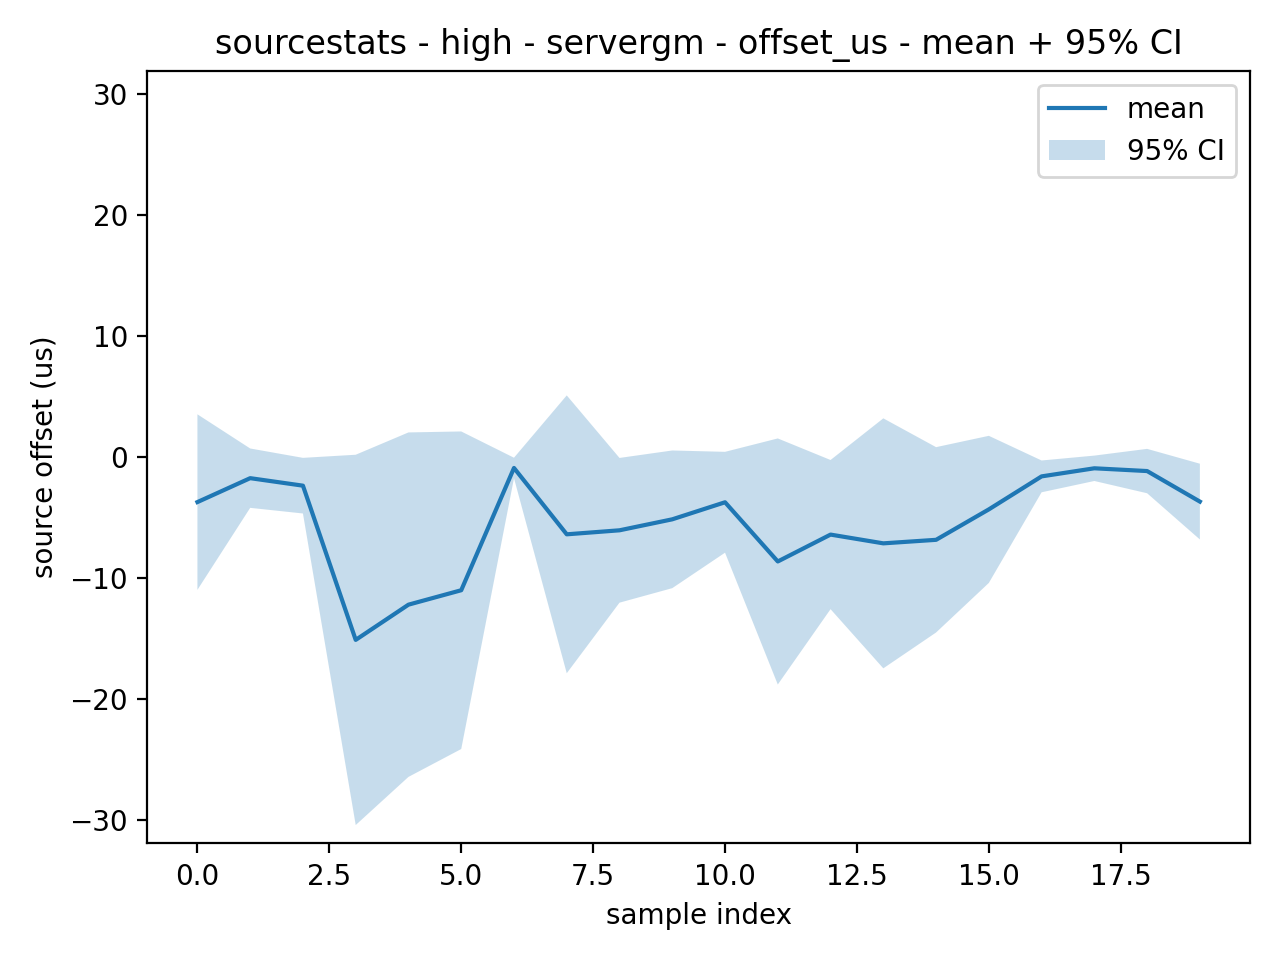
\includegraphics[width=\linewidth]{
      pars_plots/chrony_clientchrony/_aggregated/sourcestats/high/servergm/offset_us_mean_ci95.png
    }
    \caption{Scenario HIGH}
  \end{subfigure}
  \caption{Media con intervallo di confidenza al 95\% - nodo: \texttt{clientchrony}
  - netem/tc: \texttt{clientchrony}}
  \label{fig:scenario_comparison}
\end{figure}
\begin{figure}[H]
  \centering

  \begin{subfigure}
    {0.32\textwidth}
    \centering
    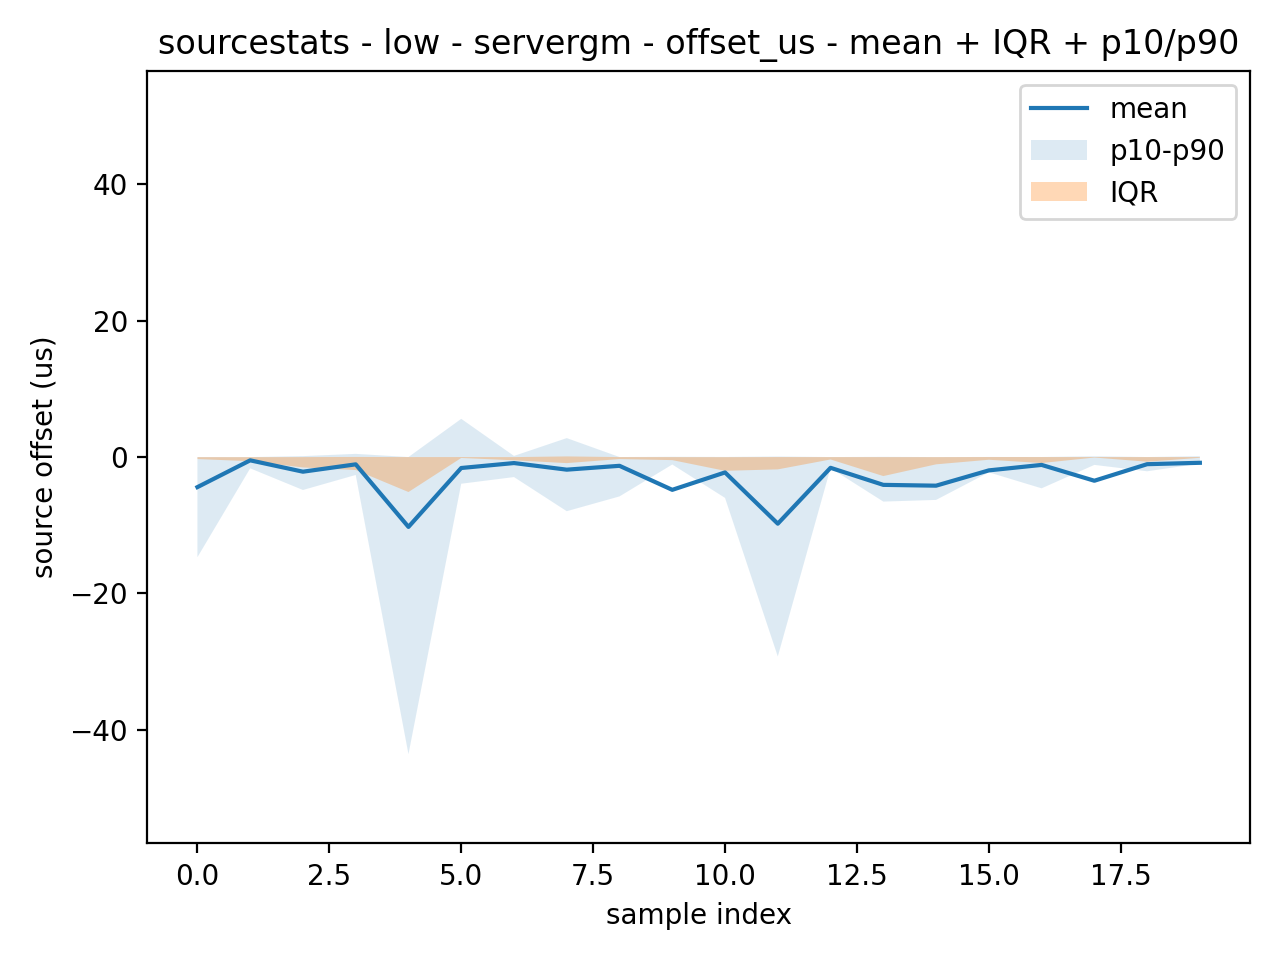
\includegraphics[width=\linewidth]{
      pars_plots/chrony_clientchrony/_aggregated/sourcestats/low/servergm/offset_us_mean_iqr_p10_p90.png
    }
    \caption{Scenario LOW}
  \end{subfigure}
  \hfill
  \begin{subfigure}
    {0.32\textwidth}
    \centering
    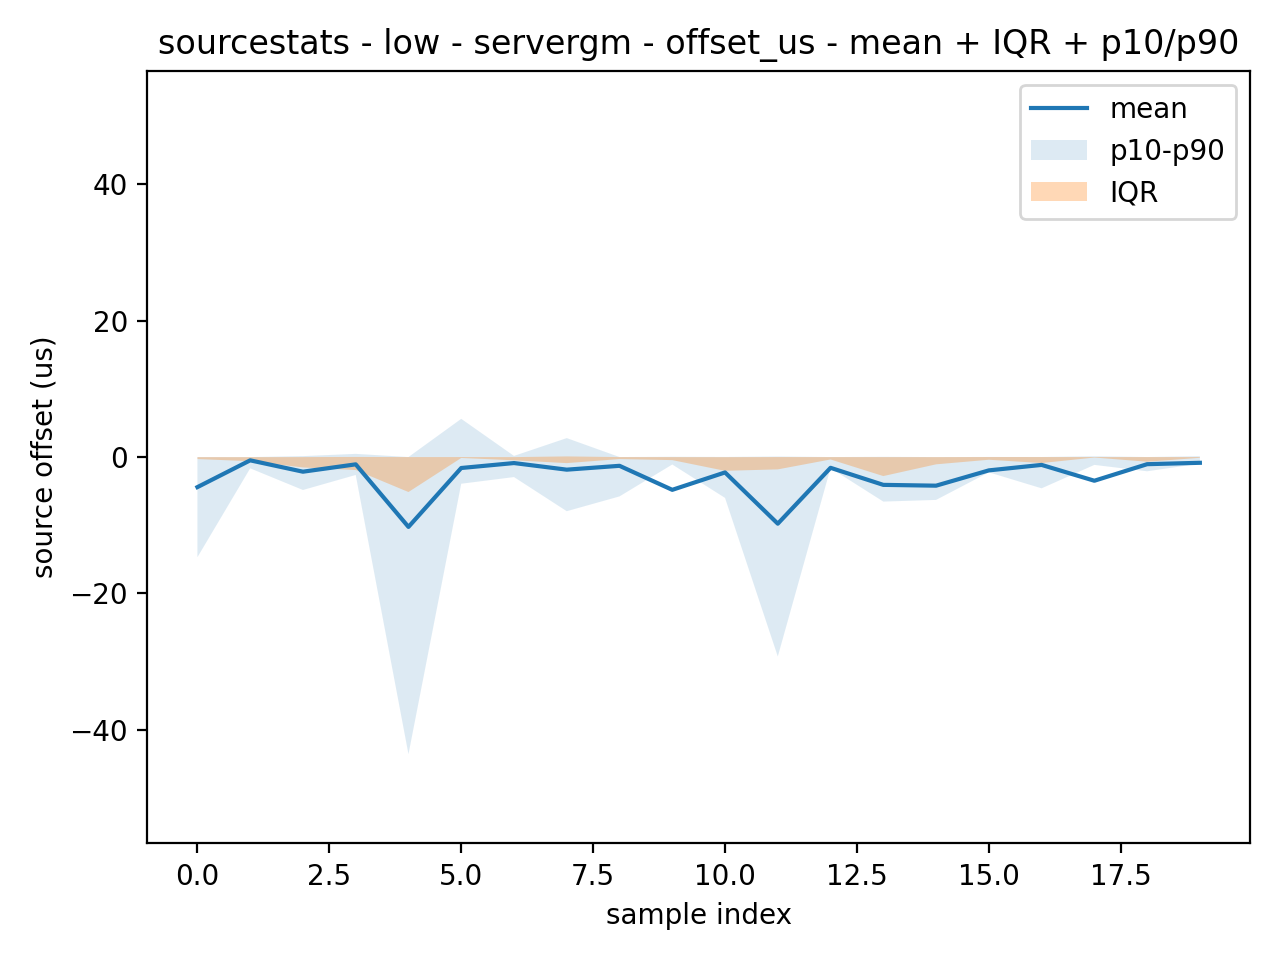
\includegraphics[width=\linewidth]{
      pars_plots/chrony_clientchrony/_aggregated/sourcestats/low/servergm/offset_us_mean_iqr_p10_p90.png
    }
    \caption{Scenario MEDIUM}
  \end{subfigure}
  \begin{subfigure}
    {0.32\textwidth}
    \centering
    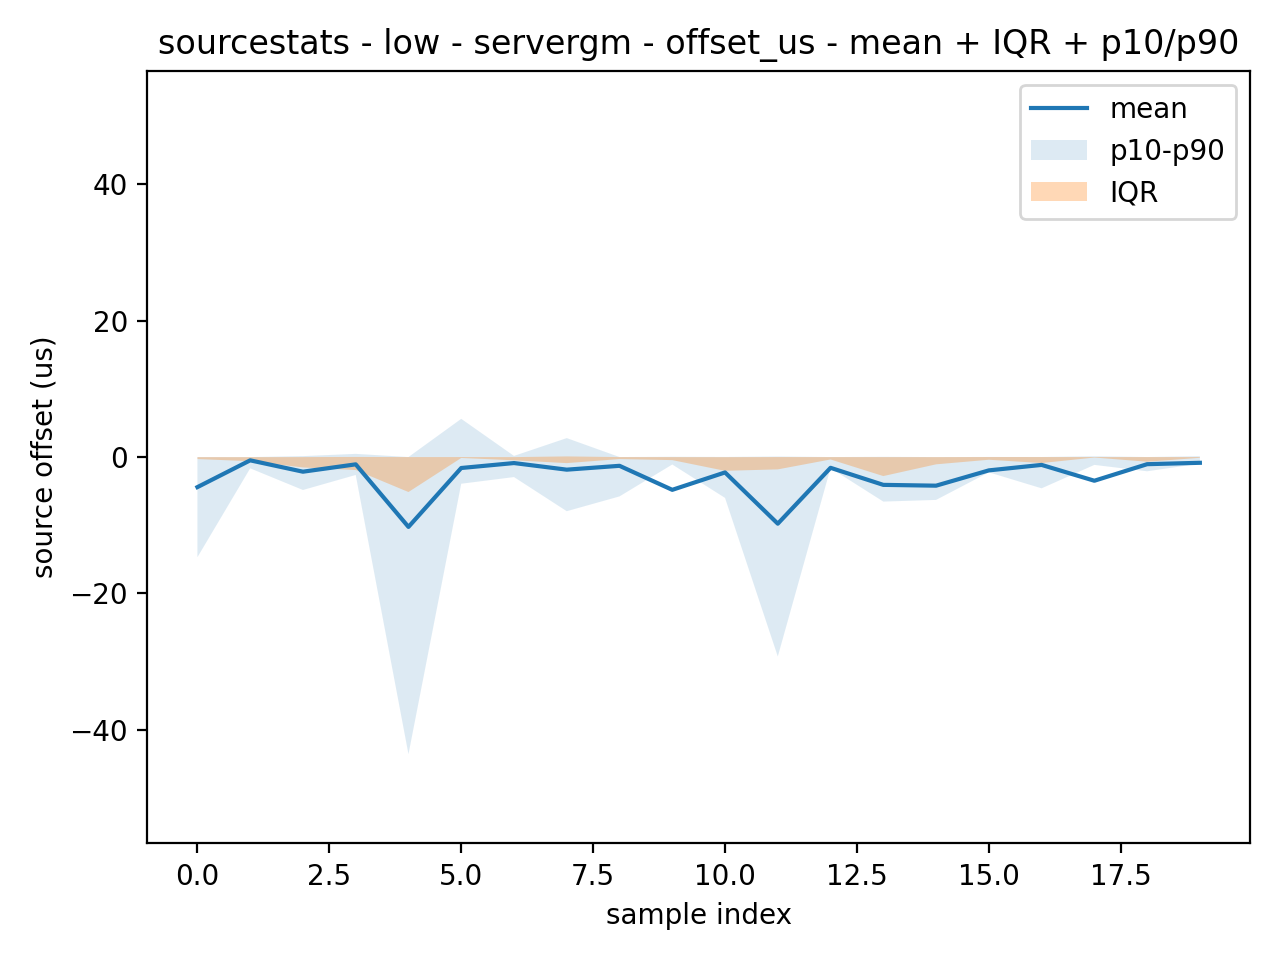
\includegraphics[width=\linewidth]{
      pars_plots/chrony_clientchrony/_aggregated/sourcestats/low/servergm/offset_us_mean_iqr_p10_p90.png
    }
    \caption{Scenario HIGH}
  \end{subfigure}
  \caption{Media con banda interquartile e banda p10-p90 - nodo: \texttt{clientchrony}
  - netem/tc: \texttt{clientchrony}}
  \label{fig:scenario_comparison}
\end{figure}
\paragraph*{clientchrony - netem/tc:}
Nel caso della metrica \texttt{offset\_us}, l'analisi relativa a \texttt{clientchrony}
con degrado applicato sul nodo client evidenzia un peggioramento progressivo all'aumentare
dell'intensità dello scenario, pur mantenendo valori complessivamente contenuti
e senza compromettere il controllo della sincronizzazione verso la sorgente.

Nello scenario \texttt{low}, la curva delle medie rimane prossima allo zero, ma con
prevalenza di valori leggermente negativi. L'aggregazione sulle curve fornisce
infatti una media complessiva pari a \texttt{-2.958 \,$\mu$s}, con valori medi
compresi tra \texttt{-10.250 \,$\mu$s} e \texttt{-0.481 \,$\mu$s}. Anche le statistiche
globali sui campioni grezzi confermano un offset generalmente molto vicino allo zero:
la media è \texttt{-2.958 \,$\mu$s}, la mediana è \texttt{-0.049 \,$\mu$s}, il
primo quartile è \texttt{-0.927 \,$\mu$s} e il terzo quartile è \texttt{-0.002 \,$\mu$s}.
Questo indica che, nella maggior parte dei campioni, lo scarto rispetto alla sorgente
rimane molto ridotto, mentre le deviazioni più marcate risultano episodiche. La variabilità
tra run non è trascurabile, come mostra l'ampiezza media dell'intervallo \texttt{p10-p90},
pari a \texttt{7.971 \,$\mu$s}, ma la banda interquartile media è molto più
contenuta, circa \texttt{1.095 \,$\mu$s}, segnalando che il comportamento tipico resta
abbastanza stabile. In termini interpretativi, nello scenario \texttt{low} il
degrado introdotto sul client produce soltanto un lieve sbilanciamento negativo
dell'offset, senza alterare in modo significativo il regime di sincronizzazione.

Nello scenario \texttt{medium}, la struttura generale del fenomeno rimane analoga,
ma la dispersione cresce leggermente e compaiono fluttuazioni negative più
frequenti. La media della curva aggregata è pari a \texttt{-2.642 \,$\mu$s}, quindi
molto vicina a quella osservata nello scenario \texttt{low}, ma i grafici mostrano
alcune discese più accentuate in specifici indici campionari. I dati grezzi
confermano che la distribuzione resta fortemente concentrata attorno a valori
prossimi allo zero: media \texttt{-2.642 \,$\mu$s}, mediana \texttt{-0.073 \,$\mu$s},
primo quartile \texttt{-1.075 \,$\mu$s} e terzo quartile \texttt{-0.004 \,$\mu$s}.
Anche in questo caso, quindi, la maggior parte delle osservazioni rimane di
piccola entità, mentre il peggioramento riguarda soprattutto la variabilità. L'ampiezza
media della banda \texttt{p10-p90} risulta pari a \texttt{6.266 \,$\mu$s}, mentre
la banda interquartile media cresce a \texttt{1.804 \,$\mu$s}; inoltre, il
valore massimo dell'IQR raggiunge \texttt{10.978 \,$\mu$s}, segnale che in
alcuni punti il comportamento tra le run diventa più irregolare. Nel complesso,
tuttavia, lo scenario \texttt{medium} non introduce una rottura netta rispetto
al caso precedente: l'offset rimane nell'ordine di pochi microsecondi negativi e continua
a descrivere un sistema sostanzialmente sotto controllo.

Nello scenario \texttt{high}, il peggioramento diventa più evidente. La media
delle curve aggregate scende a \texttt{-5.451 \,$\mu$s}, quindi circa il doppio
in valore assoluto rispetto ai casi \texttt{low} e \texttt{medium}, e la curva delle
medie mostra tratti più chiaramente distanti dallo zero, con minimi fino a
\texttt{-15.103 \,$\mu$s}. Anche i dati grezzi confermano tale tendenza: la media
globale è \texttt{-5.451 \,$\mu$s}, mentre la mediana resta comunque vicina allo zero,
pari a \texttt{-0.360 \,$\mu$s}. Questo scarto tra media e mediana è rilevante, poiché
suggerisce che il peggioramento non sia uniforme su tutti i campioni, ma sia
trainato da episodi più marcati che trascinano la media verso valori più
negativi. La dispersione aumenta sensibilmente: l'ampiezza media dell'intervallo
\texttt{p10-p90} sale a \texttt{15.836 \,$\mu$s}, quasi il doppio del caso \texttt{low},
mentre l'IQR medio raggiunge \texttt{3.693 \,$\mu$s}. Anche i grafici mostrano infatti
bande di incertezza più ampie, coerenti con una maggiore instabilità tra le run. Nonostante
ciò, il sistema non appare in collasso: l'offset rimane nell'ordine delle poche decine
di microsecondi e continua a oscillare attorno a valori compatibili con una sincronizzazione
ancora operativa, seppure meno regolare.

Nel confronto complessivo tra i tre scenari emerge dunque un andamento
progressivo. Gli scenari \texttt{low} e \texttt{medium} risultano tra loro piuttosto
vicini: in entrambi i casi l'offset medio resta attorno a \texttt{-3 \,$\mu$s} e la
maggior parte dei campioni si mantiene molto prossima allo zero. Lo scenario
\texttt{high} introduce invece un peggioramento più marcato, con media più
negativa e dispersione sensibilmente maggiore, ma senza una perdita completa di stabilità.
In sintesi, applicando il degrado di rete sul client, la metrica di \texttt{offset\_us}
verso la sorgente mostra una buona robustezza del meccanismo di sincronizzazione di
Chrony: l'effetto del degrado cresce con l'intensità dello scenario, ma rimane complessivamente
contenuto e si manifesta soprattutto come aumento della variabilità e presenza di
deviazioni negative più pronunciate, più che come deriva sistematica
incontrollata.

\begin{figure}[H]
  \centering

  \begin{subfigure}
    {0.32\textwidth}
    \centering
    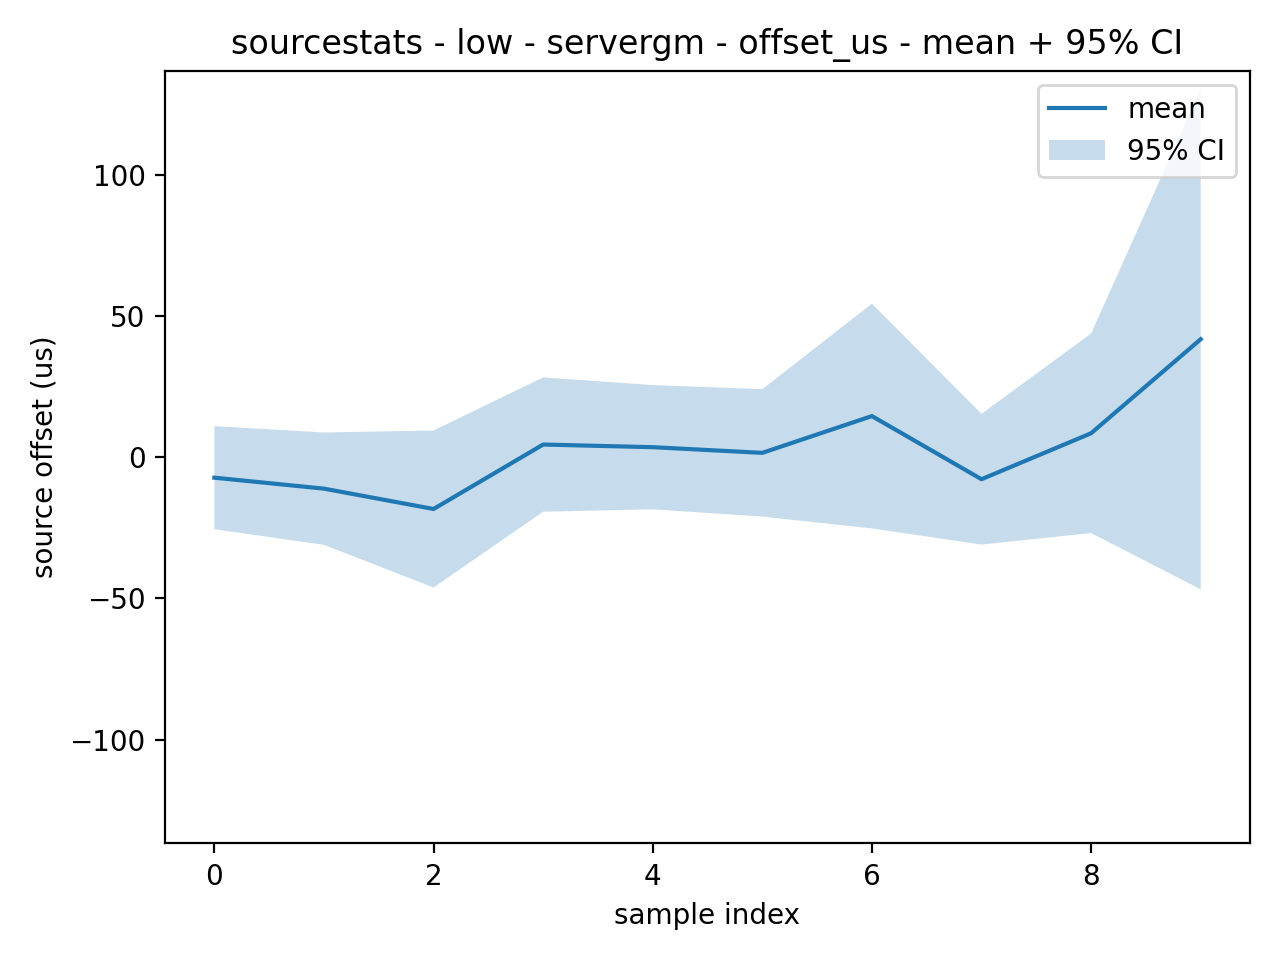
\includegraphics[width=\linewidth]{
      pars_plots/chrony_servergm/_aggregated/sourcestats/low/servergm/offset_us_mean_ci95.png
    }
    \caption{Scenario LOW}
  \end{subfigure}
  \hfill
  \begin{subfigure}
    {0.32\textwidth}
    \centering
    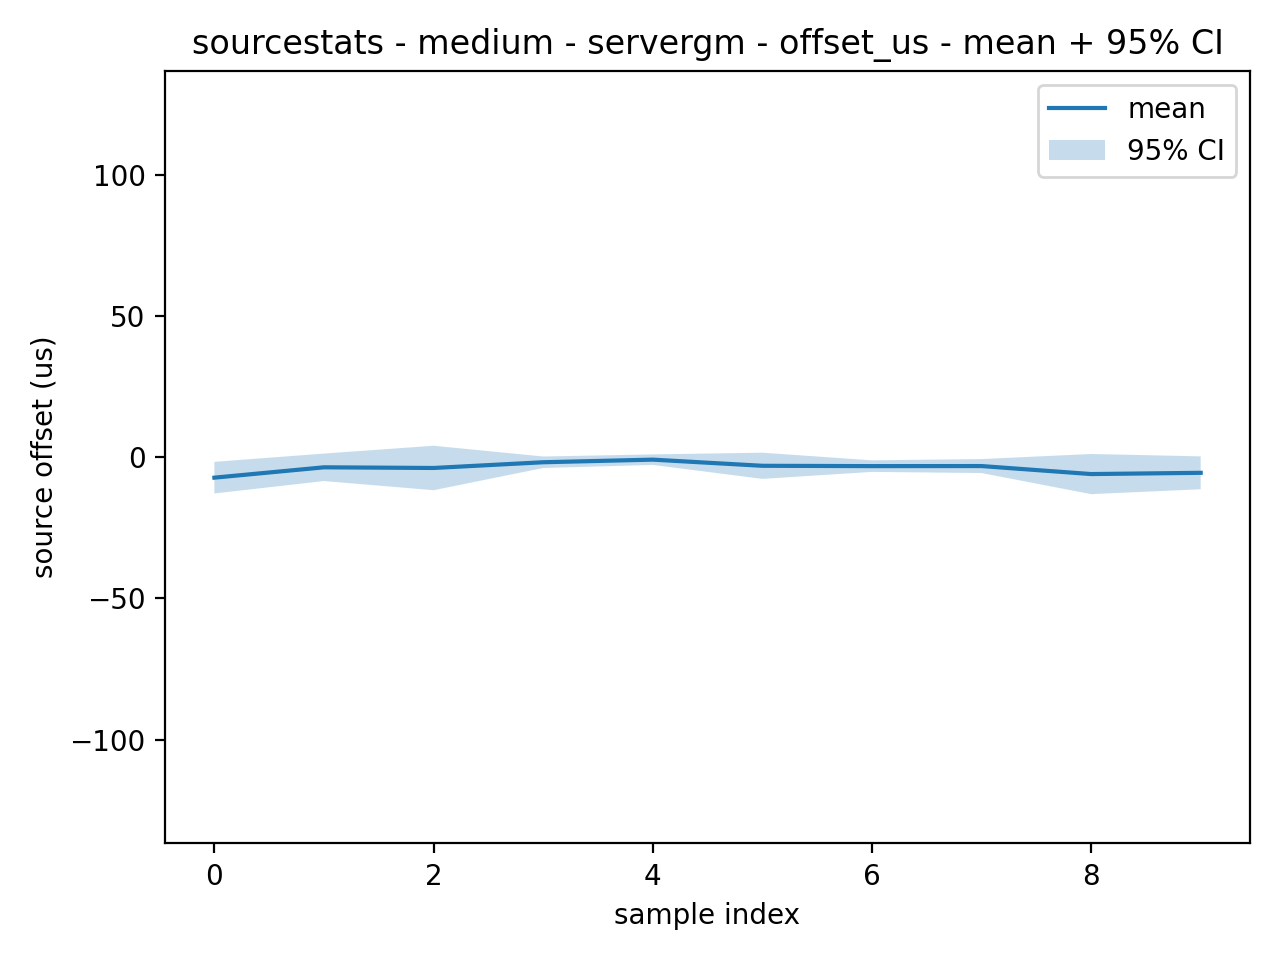
\includegraphics[width=\linewidth]{
      pars_plots/chrony_servergm/_aggregated/sourcestats/medium/servergm/offset_us_mean_ci95.png
    }
    \caption{Scenario MEDIUM}
  \end{subfigure}
  \begin{subfigure}
    {0.32\textwidth}
    \centering
    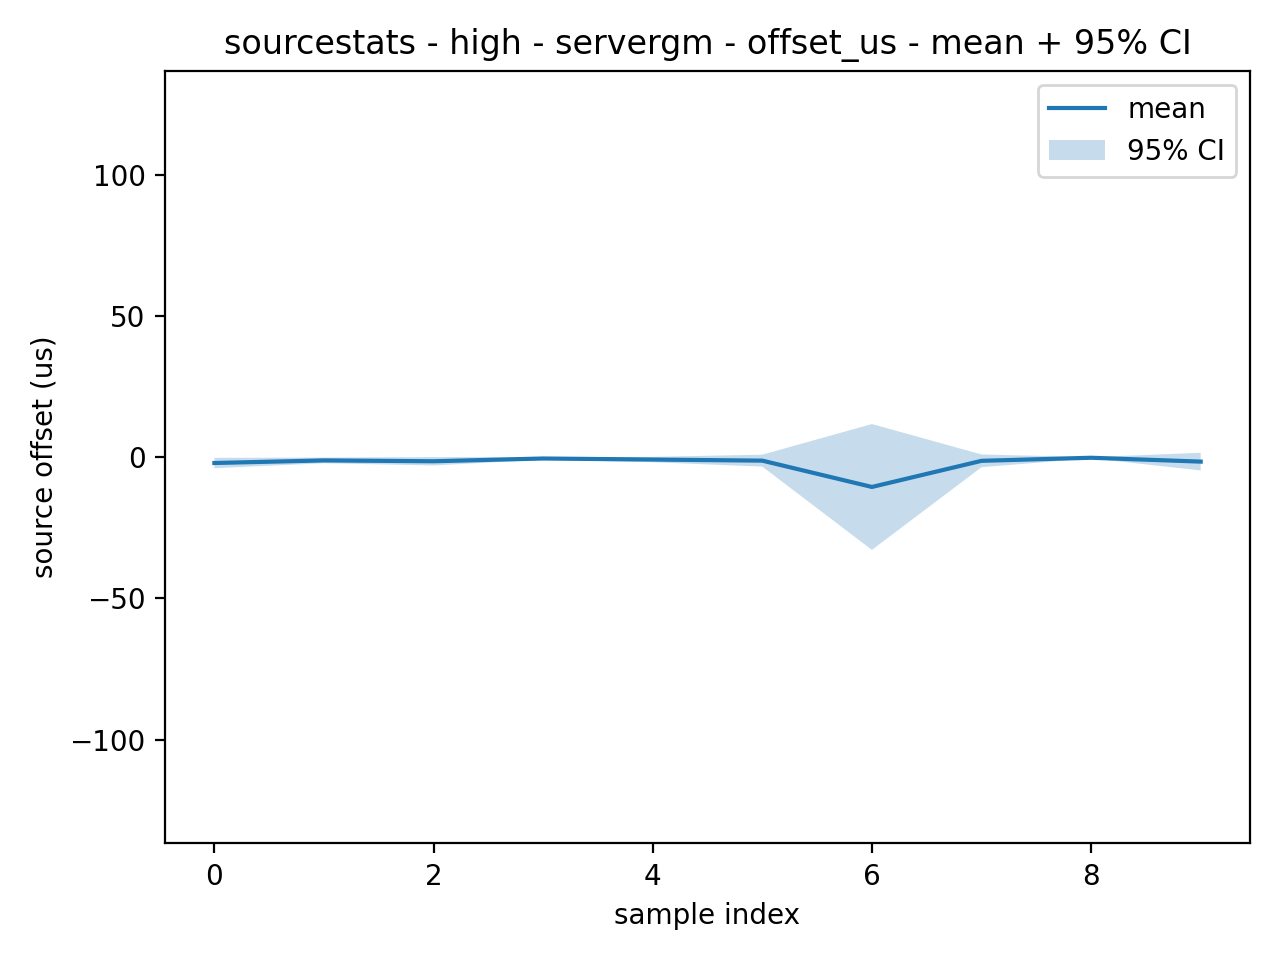
\includegraphics[width=\linewidth]{
      pars_plots/chrony_servergm/_aggregated/sourcestats/high/servergm/offset_us_mean_ci95.png
    }
    \caption{Scenario HIGH}
  \end{subfigure}
  \caption{Media con intervallo di confidenza al 95\% - nodo: \texttt{clientchrony}
  - netem/tc: \texttt{servergm}}
  \label{fig:scenario_comparison}
\end{figure}
\begin{figure}[H]
  \centering

  \begin{subfigure}
    {0.32\textwidth}
    \centering
    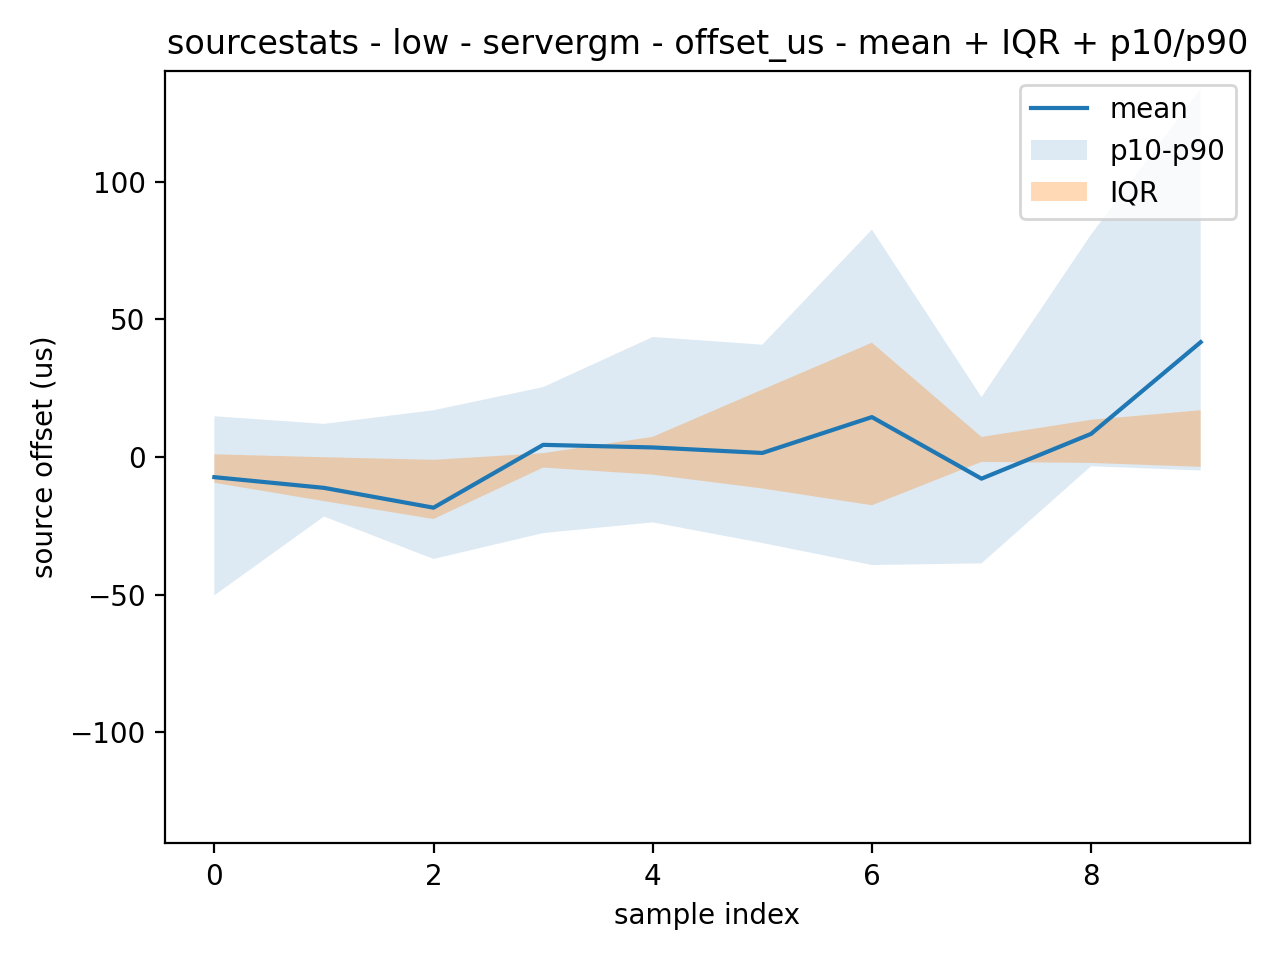
\includegraphics[width=\linewidth]{
      pars_plots/chrony_servergm/_aggregated/sourcestats/low/servergm/offset_us_mean_iqr_p10_p90.png
    }
    \caption{Scenario LOW}
  \end{subfigure}
  \hfill
  \begin{subfigure}
    {0.32\textwidth}
    \centering
    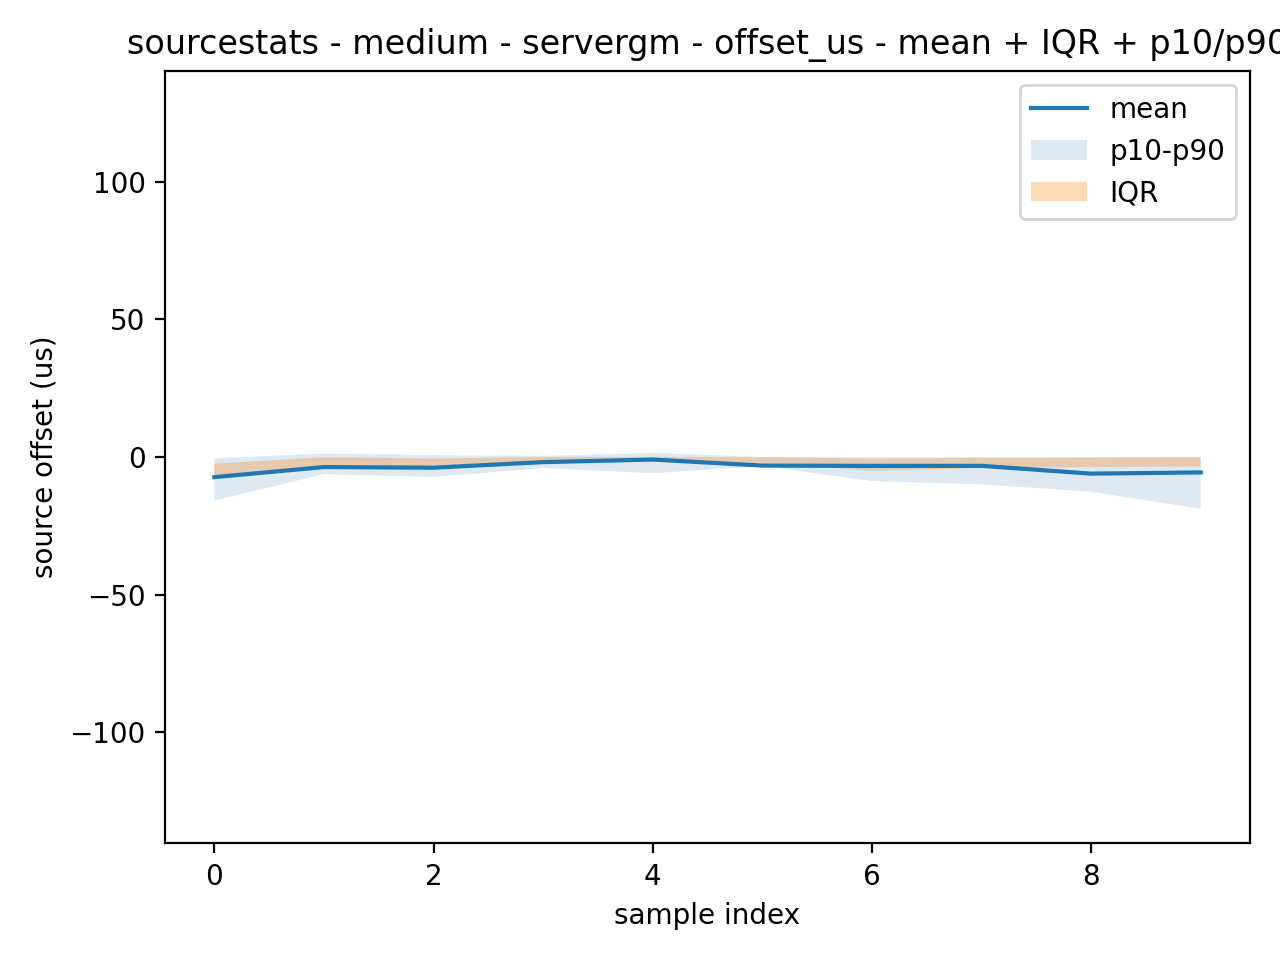
\includegraphics[width=\linewidth]{
      pars_plots/chrony_servergm/_aggregated/sourcestats/medium/servergm/offset_us_mean_iqr_p10_p90.png
    }
    \caption{Scenario MEDIUM}
  \end{subfigure}
  \begin{subfigure}
    {0.32\textwidth}
    \centering
    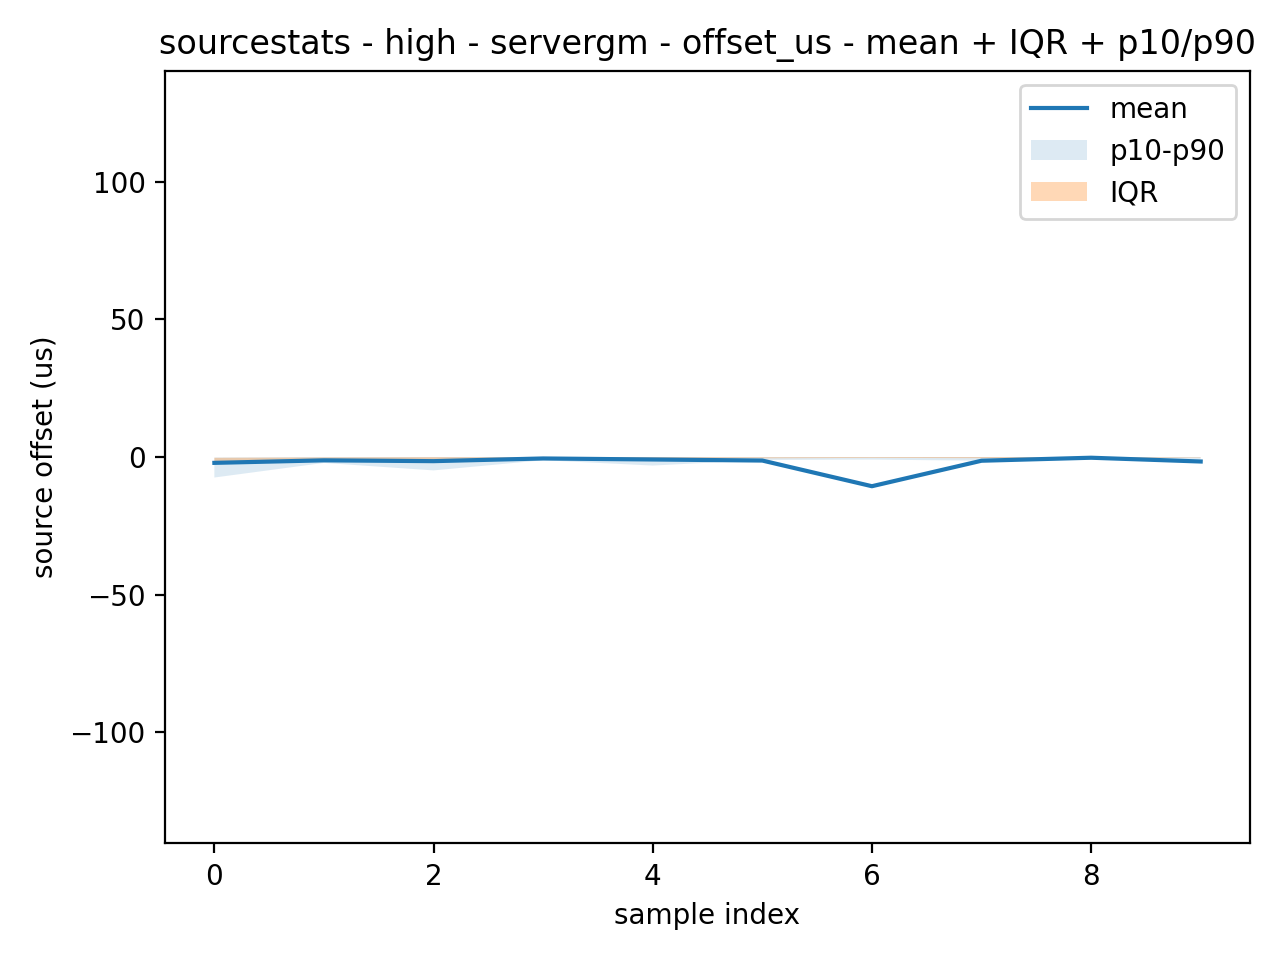
\includegraphics[width=\linewidth]{
      pars_plots/chrony_servergm/_aggregated/sourcestats/high/servergm/offset_us_mean_iqr_p10_p90.png
    }
    \caption{Scenario HIGH}
  \end{subfigure}
  \caption{Media con banda interquartile e banda p10-p90 - nodo: \texttt{clientchrony}
  - netem/tc: \texttt{servergm}}
  \label{fig:scenario_comparison}
\end{figure}
\paragraph*{servergm - netem/tc:}
Nel caso della metrica \texttt{offset\_us} riferita alla sezione \texttt{sourcestats},
l'analisi con impairment applicato sul nodo \texttt{servergm} evidenzia un comportamento
non monotono al variare dello scenario, ma nel complesso compatibile con una
sincronizzazione che resta attiva e generalmente prossima alla sorgente di
riferimento.

Nello scenario \texttt{low}, la curva delle medie presenta la maggiore
irregolarità tra i tre casi analizzati. Il valor medio aggregato risulta pari a \texttt{2.935
\,$\mu$s}, quindi molto vicino allo zero, ma la dispersione tra i diversi punti
della curva è elevata: la deviazione standard delle medie è infatti \texttt{16.824
\,$\mu$s}, con valori compresi tra \texttt{-18.383 \,$\mu$s} e \texttt{41.717 \,$\mu$s}.
Anche le bande di variabilità risultano ampie, con una larghezza media dell'intervallo
\texttt{p10-p90} pari a \texttt{74.976 \,$\mu$s} e picchi fino a \texttt{138.489
\,$\mu$s}. Le statistiche globali sui campioni grezzi confermano tale quadro: la
media complessiva è \texttt{2.935 \,$\mu$s}, ma la deviazione standard raggiunge
\texttt{68.012 \,$\mu$s}, con valori estremi fino a \texttt{555 \,$\mu$s}.
Questo indica che, pur in presenza di un valor medio contenuto, il comportamento
nello scenario \texttt{low} è caratterizzato da una marcata variabilità inter-run
e da outlier positivi che ampliano sensibilmente la dispersione osservata.

Nello scenario \texttt{medium}, la dinamica appare invece più regolare e stabile.
La curva delle medie rimane costantemente attestata su valori leggermente
negativi, con una media aggregata pari a \texttt{-3.863 \,$\mu$s}. La dispersione
si riduce in misura netta rispetto al caso precedente: la deviazione standard
delle medie scende a \texttt{1.935 \,$\mu$s}, mentre l'intervallo medio \texttt{p10-p90}
si attesta a \texttt{9.546 \,$\mu$s}. Anche le statistiche globali confermano un assetto
più compatto, con deviazione standard complessiva pari a \texttt{8.784 \,$\mu$s} e
valori estremi compresi tra \texttt{-50 \,$\mu$s} e \texttt{24 \,$\mu$s}. In
questo caso, quindi, l'offset verso la sorgente resta sistematicamente vicino
allo zero e mostra una variabilità decisamente più contenuta rispetto allo
scenario \texttt{low}.

Nello scenario \texttt{high}, il comportamento resta nel complesso stabile e,
per certi aspetti, ancora più concentrato attorno a valori prossimi allo zero.
La media aggregata della curva è pari a \texttt{-2.122 \,$\mu$s}, dunque
leggermente negativa ma di entità molto ridotta. La deviazione standard delle medie
è \texttt{3.022 \,$\mu$s}, superiore a quella osservata nello scenario \texttt{medium}
ma comunque molto inferiore al caso \texttt{low}. Inoltre, l'ampiezza media dell'IQR
è pari a soli \texttt{0.709 \,$\mu$s}, mentre l'intervallo medio \texttt{p10-p90}
è pari a \texttt{2.355 \,$\mu$s}, valori che descrivono una forte concentrazione
della parte centrale della distribuzione. I dati grezzi confermano tale lettura:
la media complessiva è \texttt{-2.122 \,$\mu$s}, con mediana \texttt{-0.178 \,$\mu$s}
e quartili molto prossimi allo zero. Nel grafico è visibile una singola
flessione più marcata, coerente con il minimo della curva pari a \texttt{-10.588 \,$\mu$s},
ma tale episodio non altera il quadro generale di sostanziale stabilità.

Nel confronto complessivo tra i tre scenari emerge dunque un risultato non lineare.
Lo scenario \texttt{low} è quello che mostra la dispersione più accentuata e la maggiore
sensibilità a valori anomali, pur mantenendo una media molto vicina allo zero. Gli
scenari \texttt{medium} e \texttt{high} appaiono invece più regolari, con offset
medi leggermente negativi ma contenuti entro pochi microsecondi e con una
variabilità sensibilmente inferiore. Pertanto, per la metrica \texttt{offset\_us}
di \texttt{sourcestats}, il degrado applicato sul nodo \texttt{servergm} non
produce una deriva sistematica progressivamente crescente al crescere dello
scenario, ma piuttosto una risposta sperimentale in cui il caso \texttt{low}
risulta il più disperso, mentre \texttt{medium} e \texttt{high} mantengono un comportamento
più compatto e vicino alla condizione nominale.

\paragraph*{Confronto:}
Nel confronto tra i due casi emerge una differenza netta nella sensibilità della
metrica \texttt{offset\_us} rispetto al punto della topologia in cui viene applicato
il degrado. Quando l'impairment è introdotto su \texttt{clientchrony}, l'effetto
sull'offset risulta più chiaramente strutturato: al crescere dello scenario si osserva
un progressivo peggioramento, con medie che si spostano verso valori più
negativi e con un aumento della dispersione, particolarmente evidente nel caso \texttt{high}.
Al contrario, con degrado applicato su \texttt{servergm}, il comportamento
appare meno regolare e non monotono: non emerge una deriva progressiva dell'offset,
ma piuttosto una risposta disomogenea, in cui lo scenario \texttt{low} risulta
paradossalmente il più disperso, mentre \texttt{medium} e \texttt{high} mantengono
un andamento più compatto e vicino alla condizione nominale.

In sintesi, il degrado applicato lato client produce un impatto più coerente e
direttamente osservabile sulla sincronizzazione stimata da Chrony, mentre il degrado
applicato lato server non determina, almeno su questa metrica, un peggioramento sistematico
crescente, ma soprattutto variazioni di dispersione tra gli scenari.

\subsection{Analisi metrica: \texttt{stddev}}
\begin{figure}[H]
  \centering

  \begin{subfigure}
    {0.32\textwidth}
    \centering
    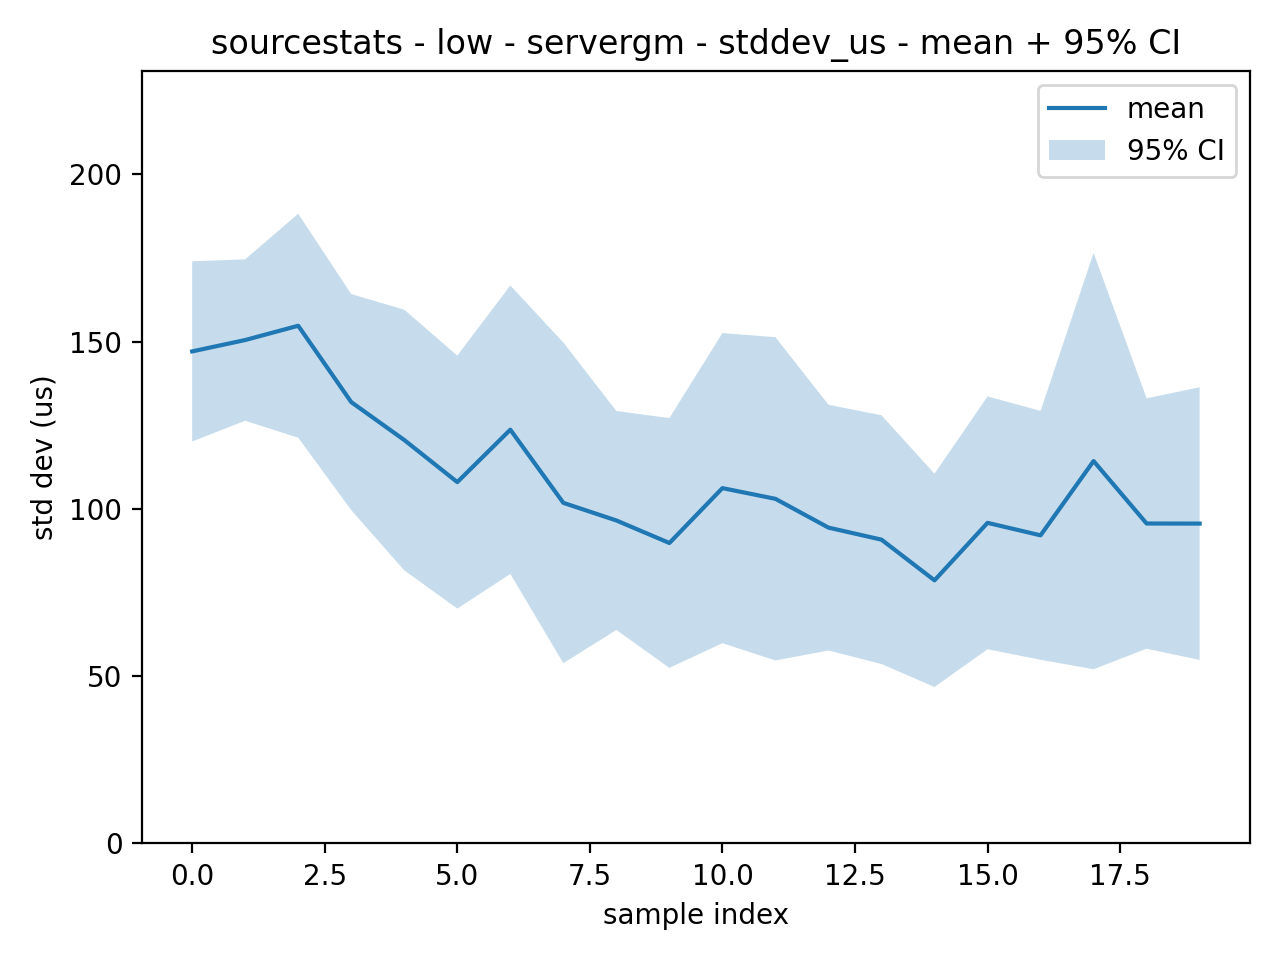
\includegraphics[width=\linewidth]{
      pars_plots/chrony_clientchrony/_aggregated/sourcestats/low/servergm/stddev_us_mean_ci95.png
    }
    \caption{Scenario LOW}
  \end{subfigure}
  \hfill
  \begin{subfigure}
    {0.32\textwidth}
    \centering
    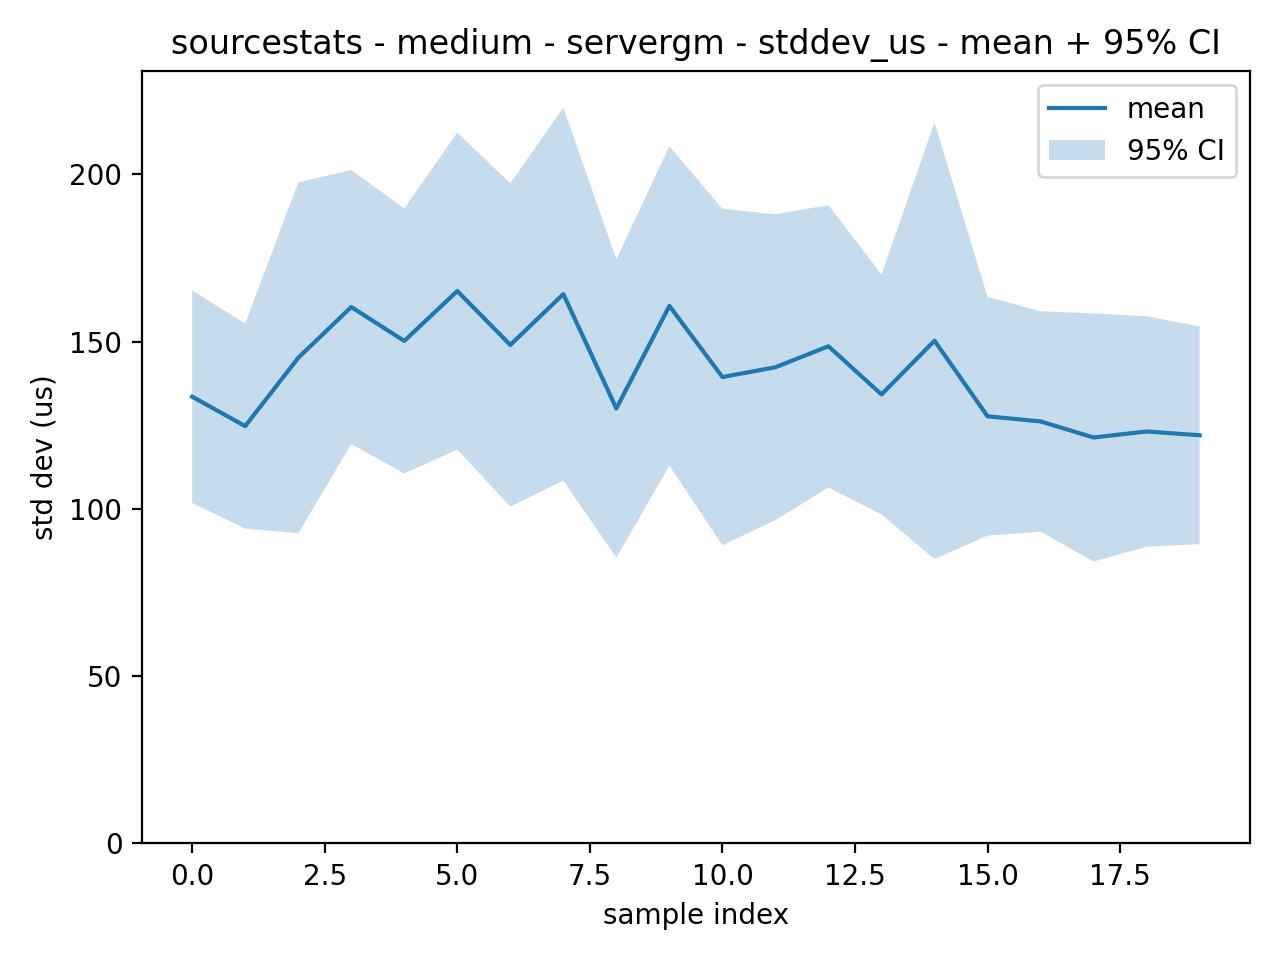
\includegraphics[width=\linewidth]{
      pars_plots/chrony_clientchrony/_aggregated/sourcestats/medium/servergm/stddev_us_mean_ci95.png
    }
    \caption{Scenario MEDIUM}
  \end{subfigure}
  \begin{subfigure}
    {0.32\textwidth}
    \centering
    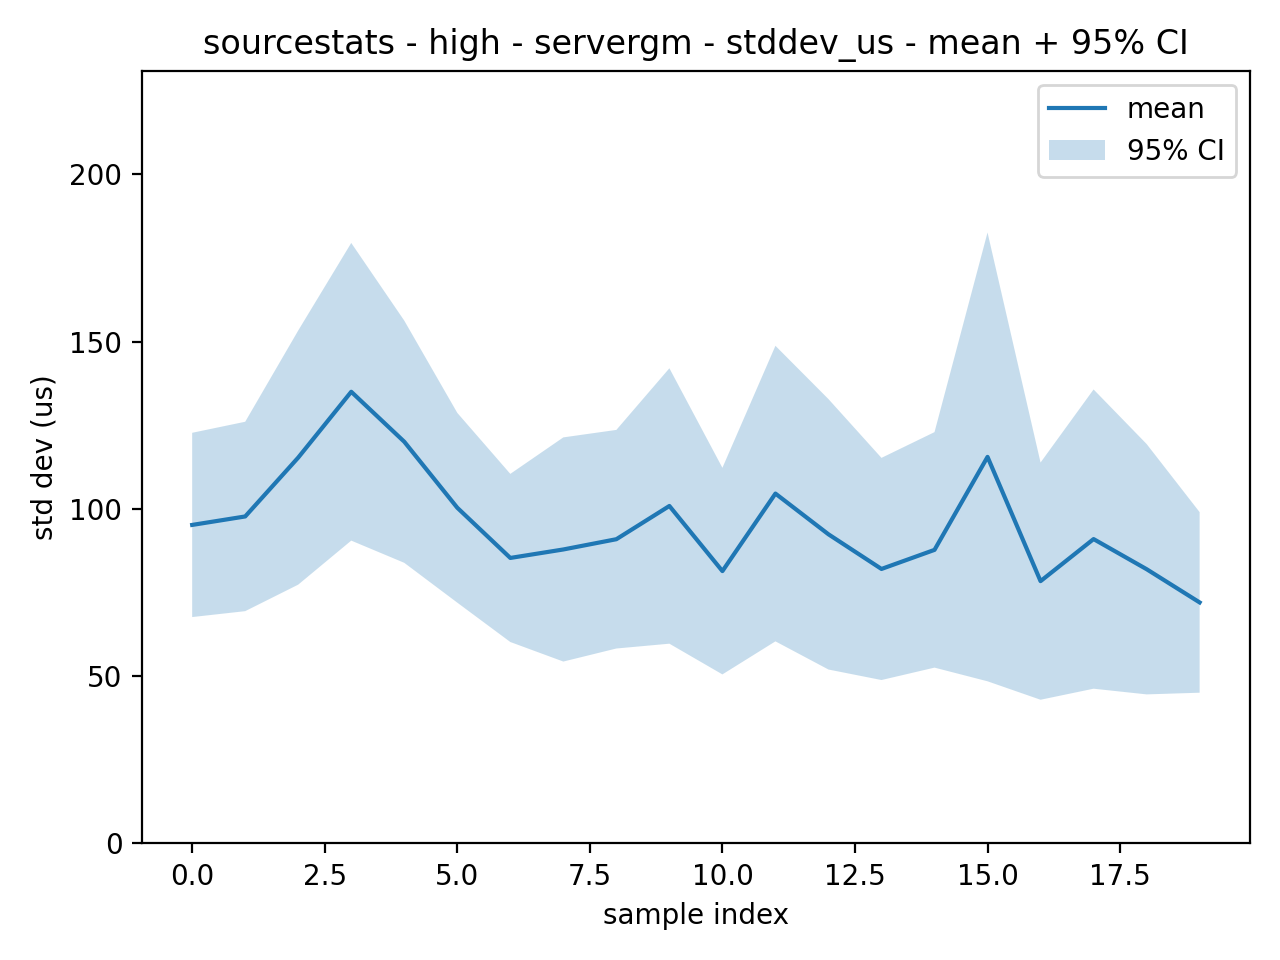
\includegraphics[width=\linewidth]{
      pars_plots/chrony_clientchrony/_aggregated/sourcestats/high/servergm/stddev_us_mean_ci95.png
    }
    \caption{Scenario HIGH}
  \end{subfigure}
  \caption{Media con intervallo di confidenza al 95\% - nodo: \texttt{clientchrony}
  - netem/tc: \texttt{clientchrony}}
  \label{fig:scenario_comparison}
\end{figure}
\begin{figure}[H]
  \centering

  \begin{subfigure}
    {0.32\textwidth}
    \centering
    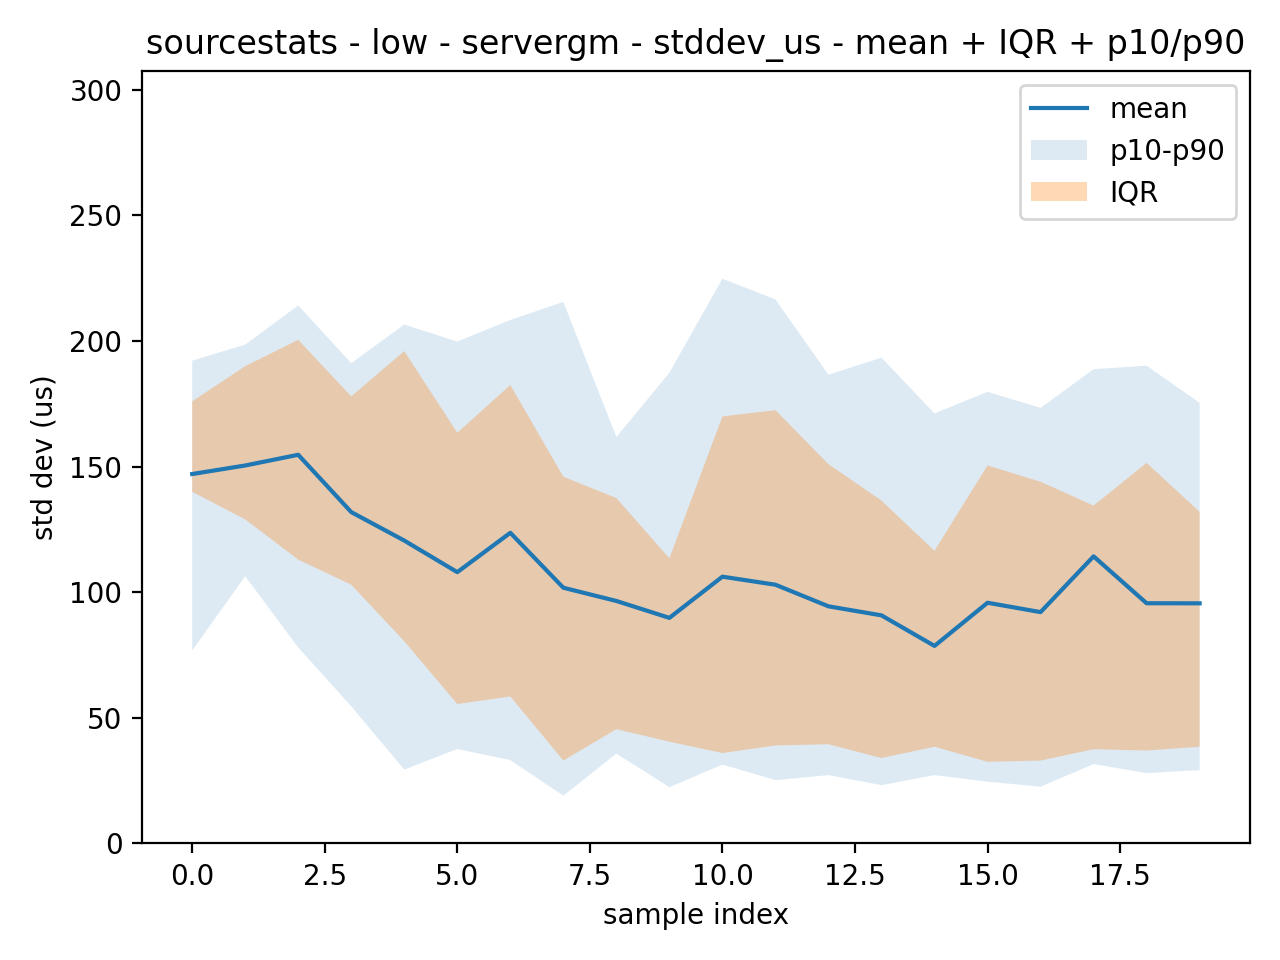
\includegraphics[width=\linewidth]{
      pars_plots/chrony_clientchrony/_aggregated/sourcestats/low/servergm/stddev_us_mean_iqr_p10_p90.png
    }
    \caption{Scenario LOW}
  \end{subfigure}
  \hfill
  \begin{subfigure}
    {0.32\textwidth}
    \centering
    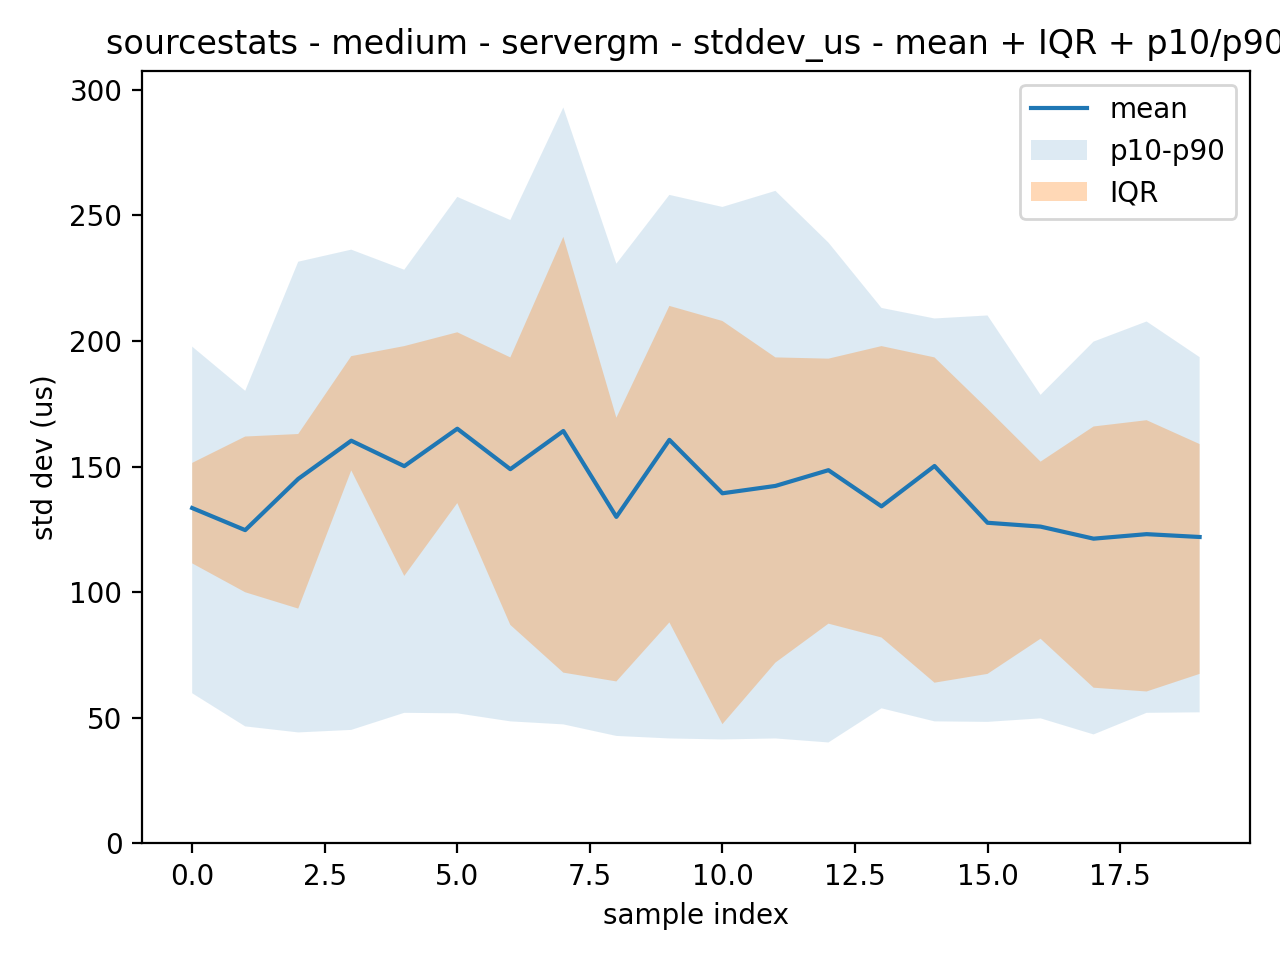
\includegraphics[width=\linewidth]{
      pars_plots/chrony_clientchrony/_aggregated/sourcestats/medium/servergm/stddev_us_mean_iqr_p10_p90.png
    }
    \caption{Scenario MEDIUM}
  \end{subfigure}
  \begin{subfigure}
    {0.32\textwidth}
    \centering
    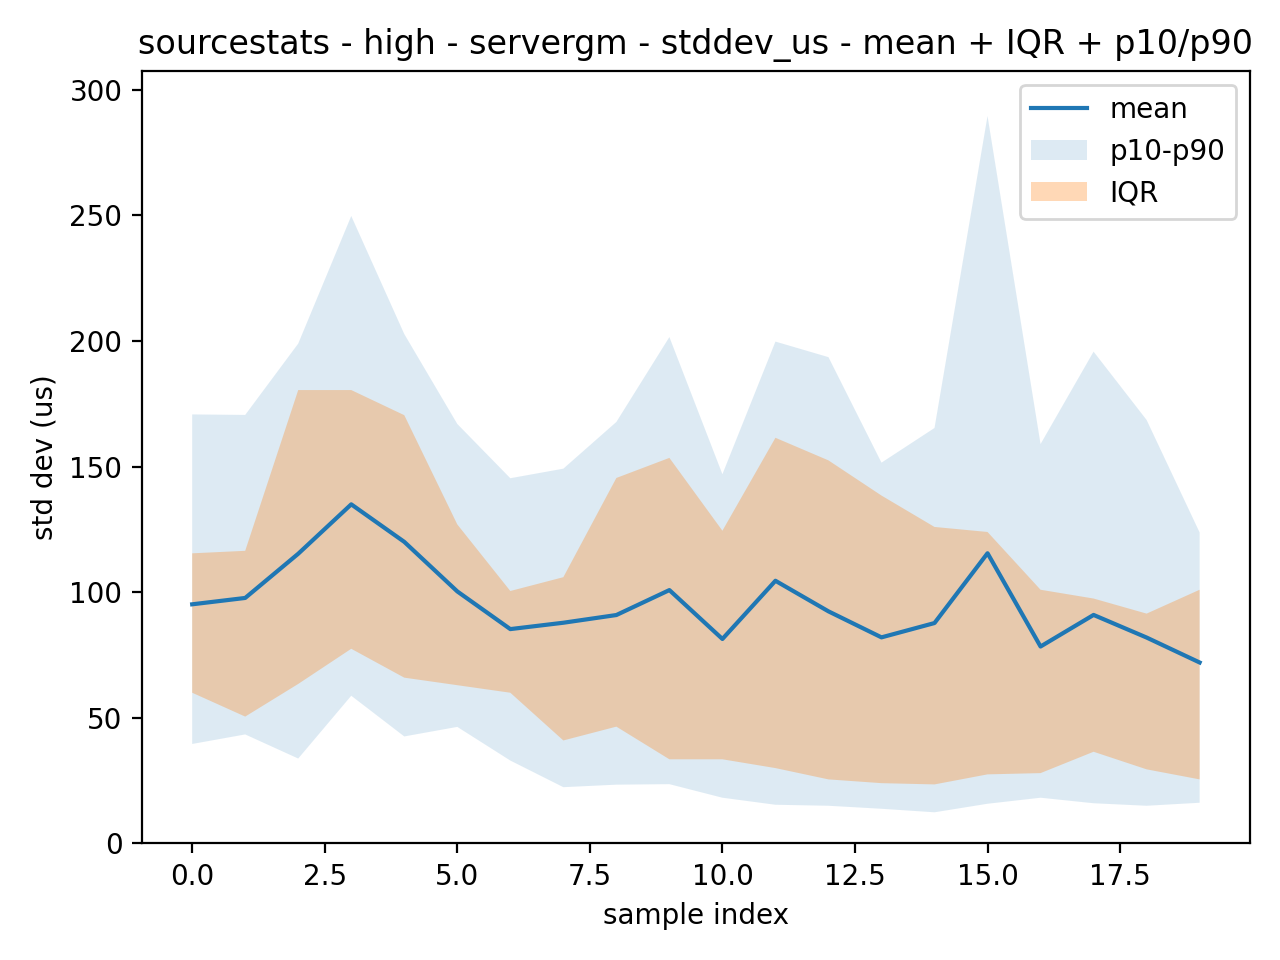
\includegraphics[width=\linewidth]{
      pars_plots/chrony_clientchrony/_aggregated/sourcestats/high/servergm/stddev_us_mean_iqr_p10_p90.png
    }
    \caption{Scenario HIGH}
  \end{subfigure}
  \caption{Media con banda interquartile e banda p10-p90 - nodo: \texttt{clientchrony}
  - netem/tc: \texttt{clientchrony}}
  \label{fig:scenario_comparison}
\end{figure}
\paragraph*{clientchrony - netem/tc:}
Nel caso della metrica \texttt{stddev\_us}, l'analisi relativa a \texttt{clientchrony}
con degrado applicato sul nodo client non mostra un peggioramento monotono al
crescere dell'intensità dello scenario, ma piuttosto una risposta non lineare della
variabilità stimata rispetto alla sorgente. In tutti i casi i valori restano
dell'ordine delle centinaia di microsecondi, ma con differenze apprezzabili sia nel
livello medio sia nella regolarità tra i diversi scenari.

Nello scenario \texttt{low}, la curva delle medie si colloca su un livello complessivamente
intermedio, con una media aggregata pari a \texttt{109.552 \,$\mu$s}. La
dinamica mostra una discesa nella prima parte della curva, passando da valori iniziali
prossimi a \texttt{150 \,$\mu$s} verso livelli più vicini a \texttt{90{-}100 \,$\mu$s},
per poi mantenersi relativamente stabile con alcune oscillazioni locali. La dispersione
lungo la curva non è trascurabile: la deviazione standard delle medie è \texttt{21.838
\,$\mu$s}, con valori compresi tra \texttt{78.637 \,$\mu$s} e \texttt{154.733 \,$\mu$s}.
Anche le bande di variabilità sono ampie, con IQR medio pari a \texttt{98.925 \,$\mu$s}
e ampiezza media \texttt{p10-p90} pari a \texttt{155.630 \,$\mu$s}. Le
statistiche globali sui campioni grezzi confermano il medesimo ordine di
grandezza: media \texttt{109.552 \,$\mu$s}, mediana \texttt{103 \,$\mu$s}, terzo quartile
\texttt{167 \,$\mu$s} e massimo \texttt{464 \,$\mu$s}. Nel complesso, quindi, lo
scenario \texttt{low} descrive una variabilità della sorgente stimata già significativa,
ma ancora distribuita in modo relativamente regolare lungo la curva.

Nello scenario \texttt{medium}, la metrica cresce in modo netto e si porta sul
livello più elevato tra i tre casi osservati. La media aggregata raggiunge infatti
\texttt{140.899 \,$\mu$s}, con mediana della curva pari a \texttt{140.867 \,$\mu$s}
e valori medi che oscillano tra \texttt{121.333 \,$\mu$s} e \texttt{165.109 \,$\mu$s}.
Anche visivamente la curva appare attestata su un piano superiore rispetto a quello
dei casi \texttt{low} e \texttt{high}. La dispersione tra i punti della curva, pur
non esplodendo, resta presente: la deviazione standard delle medie è \texttt{14.774
\,$\mu$s}. Le bande di variabilità risultano tuttavia più larghe del caso \texttt{low}:
l'IQR medio sale a \texttt{100.000 \,$\mu$s} e l'ampiezza media \texttt{p10-p90} raggiunge
\texttt{178.740 \,$\mu$s}. Le statistiche globali confermano questa configurazione,
con media complessiva \texttt{140.899 \,$\mu$s}, mediana \texttt{141 \,$\mu$s},
terzo quartile \texttt{191.250 \,$\mu$s} e massimo \texttt{510 \,$\mu$s}. Lo scenario
\texttt{medium} rappresenta quindi il caso in cui la stima di dispersione della
sorgente risulta mediamente più alta, pur senza mostrare instabilità irregolari particolarmente
marcate nella curva delle medie.

Nello scenario \texttt{high}, il livello medio della metrica diminuisce sensibilmente
rispetto al caso \texttt{medium} e si colloca anche al di sotto del caso \texttt{low}.
La media aggregata della curva è pari a \texttt{95.787 \,$\mu$s}, con mediana
\texttt{91.687 \,$\mu$s} e valori compresi tra \texttt{72.040 \,$\mu$s} e
\texttt{135.000 \,$\mu$s}. La curva appare più irregolare di quella osservata in
\texttt{medium}, ma resta comunque confinata entro un intervallo relativamente
contenuto. Le bande di variabilità rimangono ampie: l'IQR medio vale \texttt{88.450
\,$\mu$s}, mentre l'ampiezza media \texttt{p10-p90} è pari a \texttt{154.760 \,$\mu$s},
dunque molto vicina al caso \texttt{low} ma inferiore al caso \texttt{medium}.
Anche i dati grezzi confermano tale riduzione del livello medio, con media complessiva
\texttt{95.787 \,$\mu$s}, mediana \texttt{88 \,$\mu$s} e massimo \texttt{410 \,$\mu$s}.
In questo scenario, quindi, non si osserva un ulteriore aumento della
variabilità stimata, bensì un ritorno verso valori medi più bassi.

Nel confronto complessivo tra i tre scenari emerge dunque un andamento non monotono.
Lo scenario \texttt{medium} è quello che presenta il livello medio più elevato della
metrica \texttt{stddev\_us}, mentre \texttt{low} occupa una posizione intermedia
e \texttt{high} mostra invece valori medi più contenuti. Anche sul piano della
dispersione intra-curva e inter-run non si osserva una crescita progressiva con
l'intensità del degrado: le bande restano ampie in tutti i casi, ma raggiungono
i valori medi più elevati ancora nello scenario \texttt{medium}. Pertanto, per questa
metrica, il degrado applicato su \texttt{clientchrony} non produce una risposta semplicemente
crescente, ma modifica la stima della deviazione standard in modo più articolato,
con un massimo nel caso \texttt{medium} e un successivo ridimensionamento nel
caso \texttt{high}.

\begin{figure}[H]
  \centering

  \begin{subfigure}
    {0.32\textwidth}
    \centering
    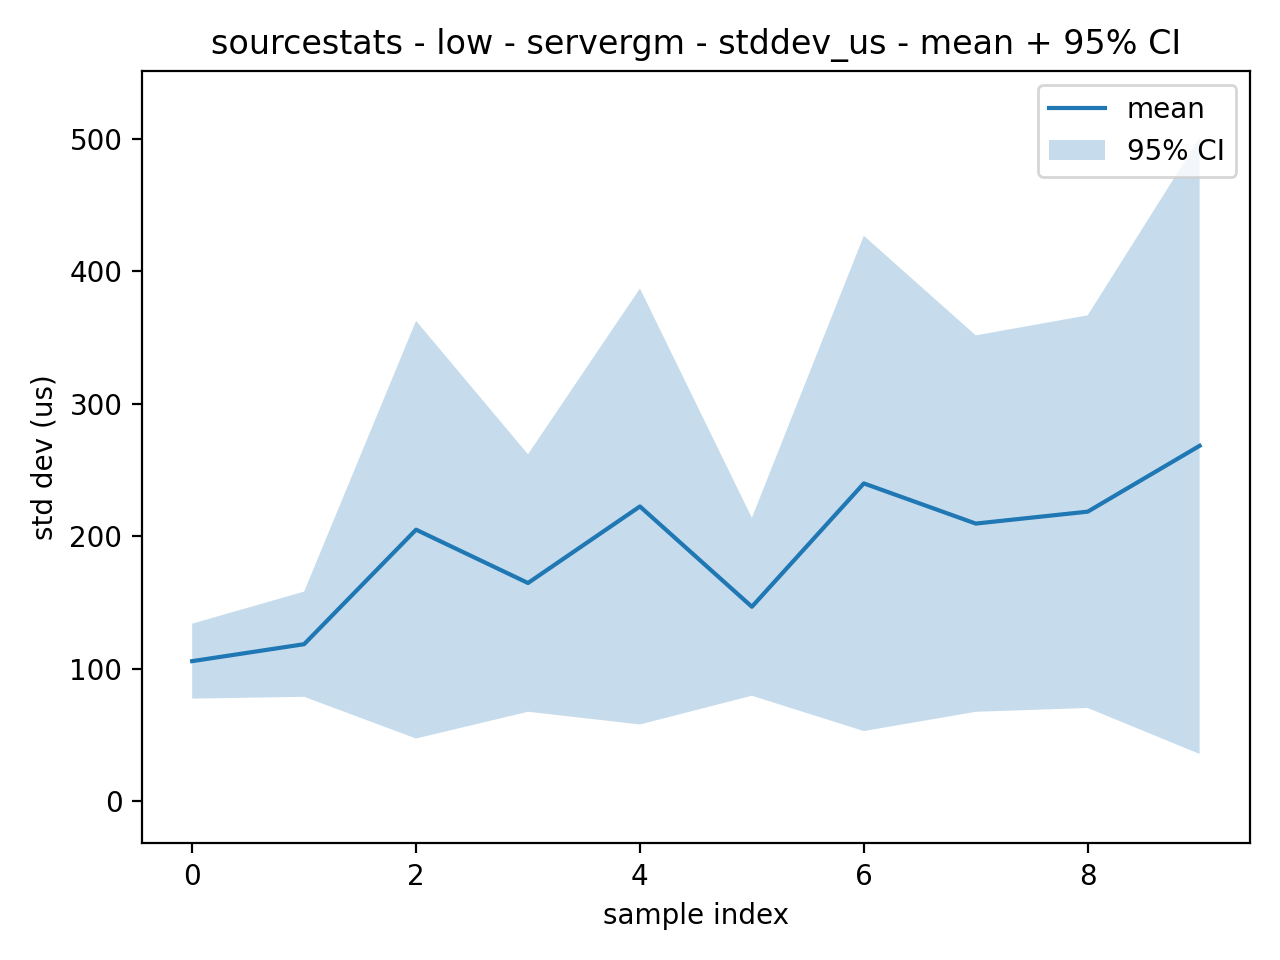
\includegraphics[width=\linewidth]{
      pars_plots/chrony_servergm/_aggregated/sourcestats/low/servergm/stddev_us_mean_ci95.png
    }
    \caption{Scenario LOW}
  \end{subfigure}
  \hfill
  \begin{subfigure}
    {0.32\textwidth}
    \centering
    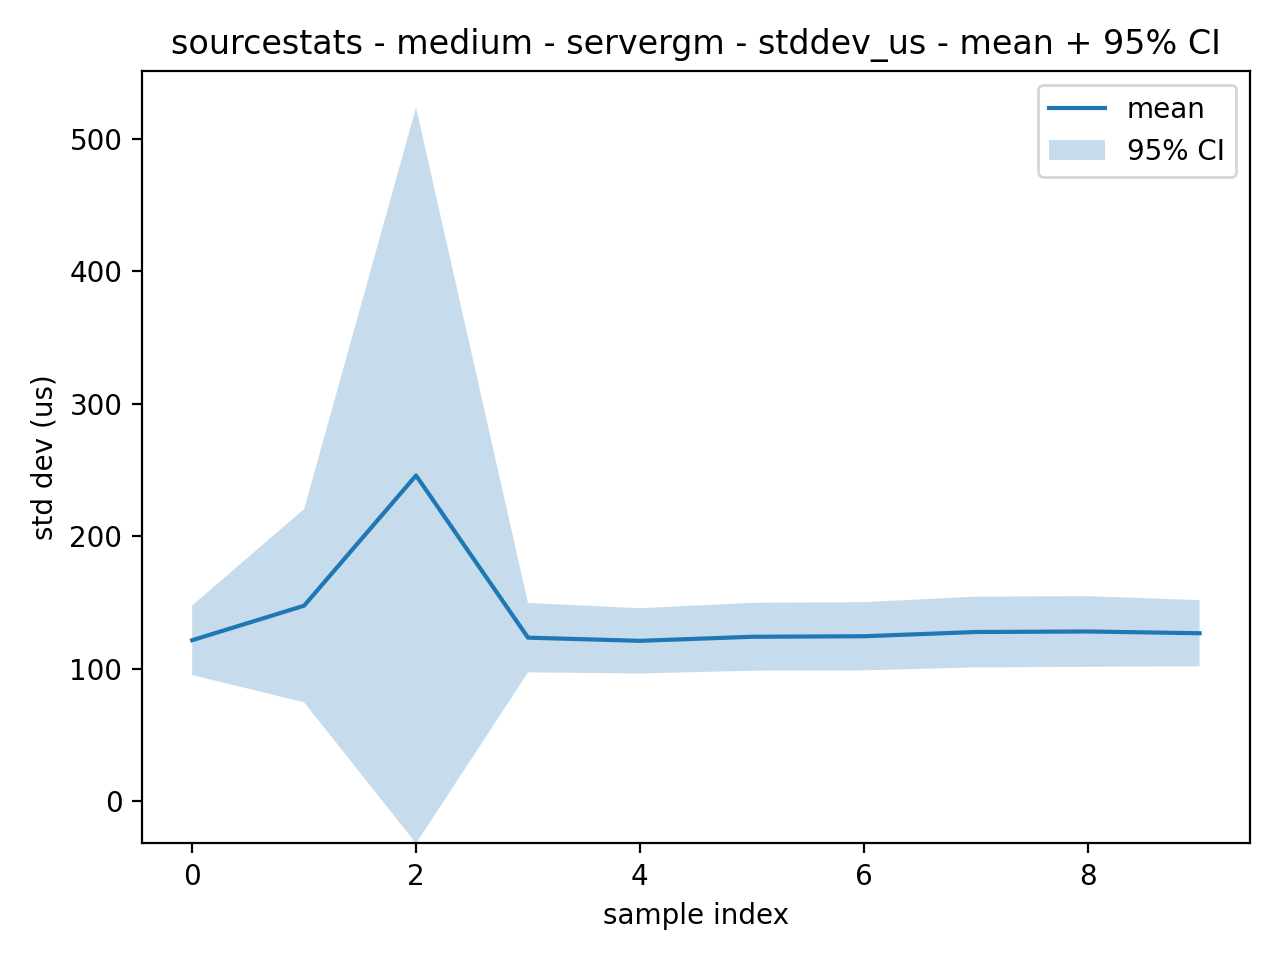
\includegraphics[width=\linewidth]{
      pars_plots/chrony_servergm/_aggregated/sourcestats/medium/servergm/stddev_us_mean_ci95.png
    }
    \caption{Scenario MEDIUM}
  \end{subfigure}
  \begin{subfigure}
    {0.32\textwidth}
    \centering
    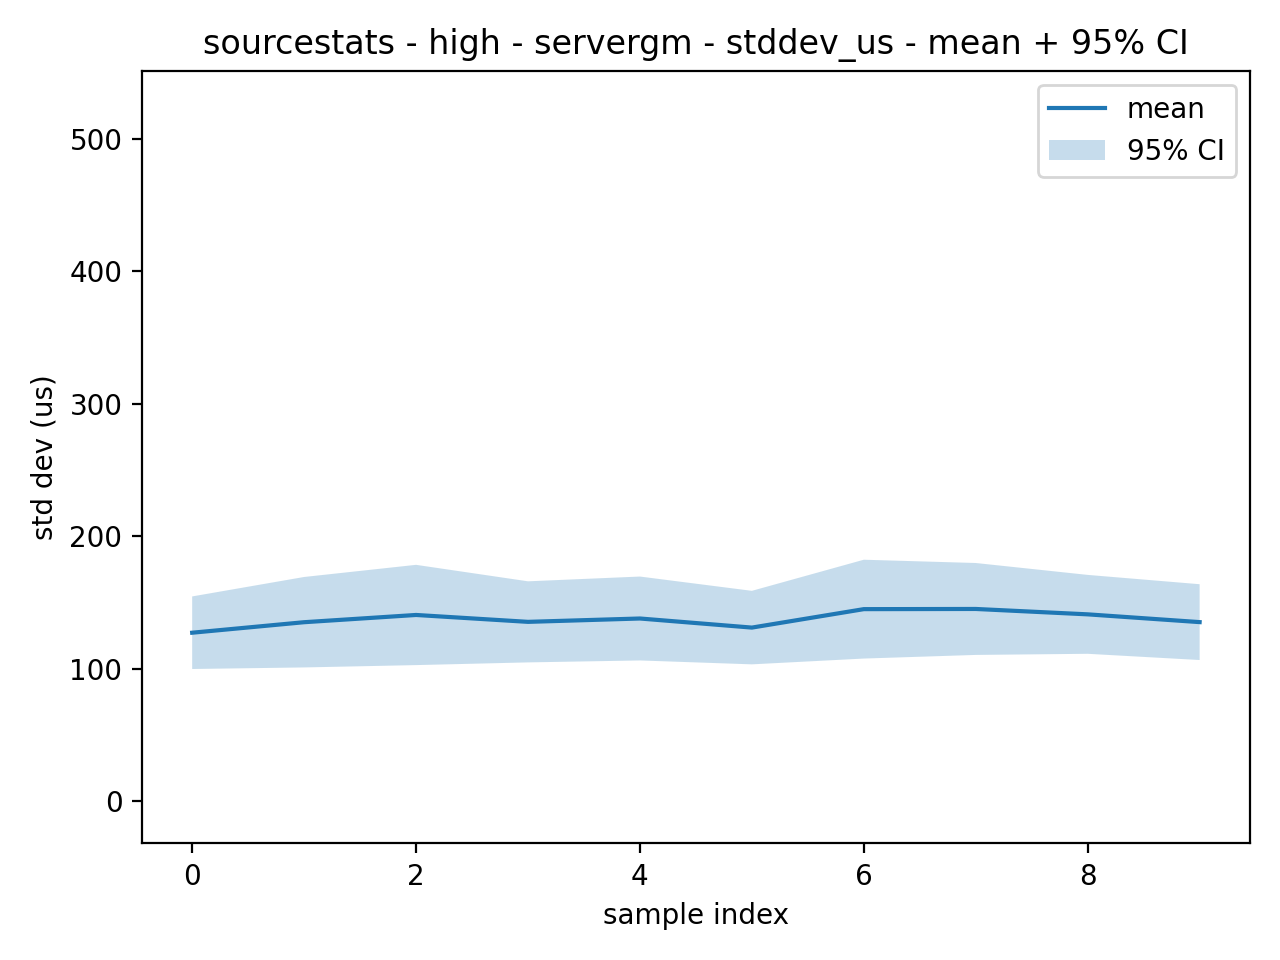
\includegraphics[width=\linewidth]{
      pars_plots/chrony_servergm/_aggregated/sourcestats/high/servergm/stddev_us_mean_ci95.png
    }
    \caption{Scenario HIGH}
  \end{subfigure}
  \caption{Media con intervallo di confidenza al 95\% - nodo: \texttt{clientchrony}
  - netem/tc: \texttt{servergm}}
  \label{fig:scenario_comparison}
\end{figure}
\begin{figure}[H]
  \centering

  \begin{subfigure}
    {0.32\textwidth}
    \centering
    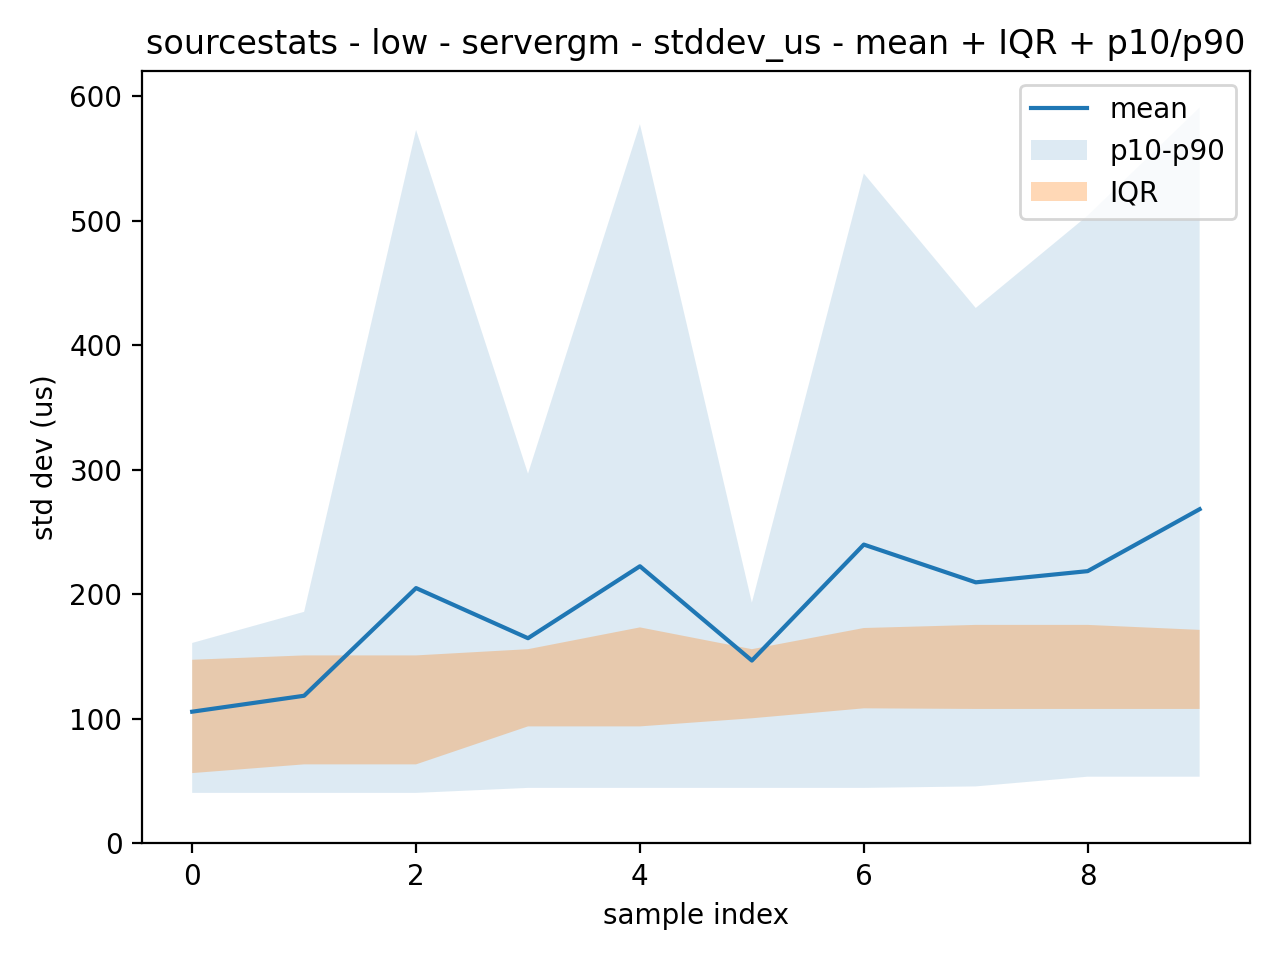
\includegraphics[width=\linewidth]{
      pars_plots/chrony_servergm/_aggregated/sourcestats/low/servergm/stddev_us_mean_iqr_p10_p90.png
    }
    \caption{Scenario LOW}
  \end{subfigure}
  \hfill
  \begin{subfigure}
    {0.32\textwidth}
    \centering
    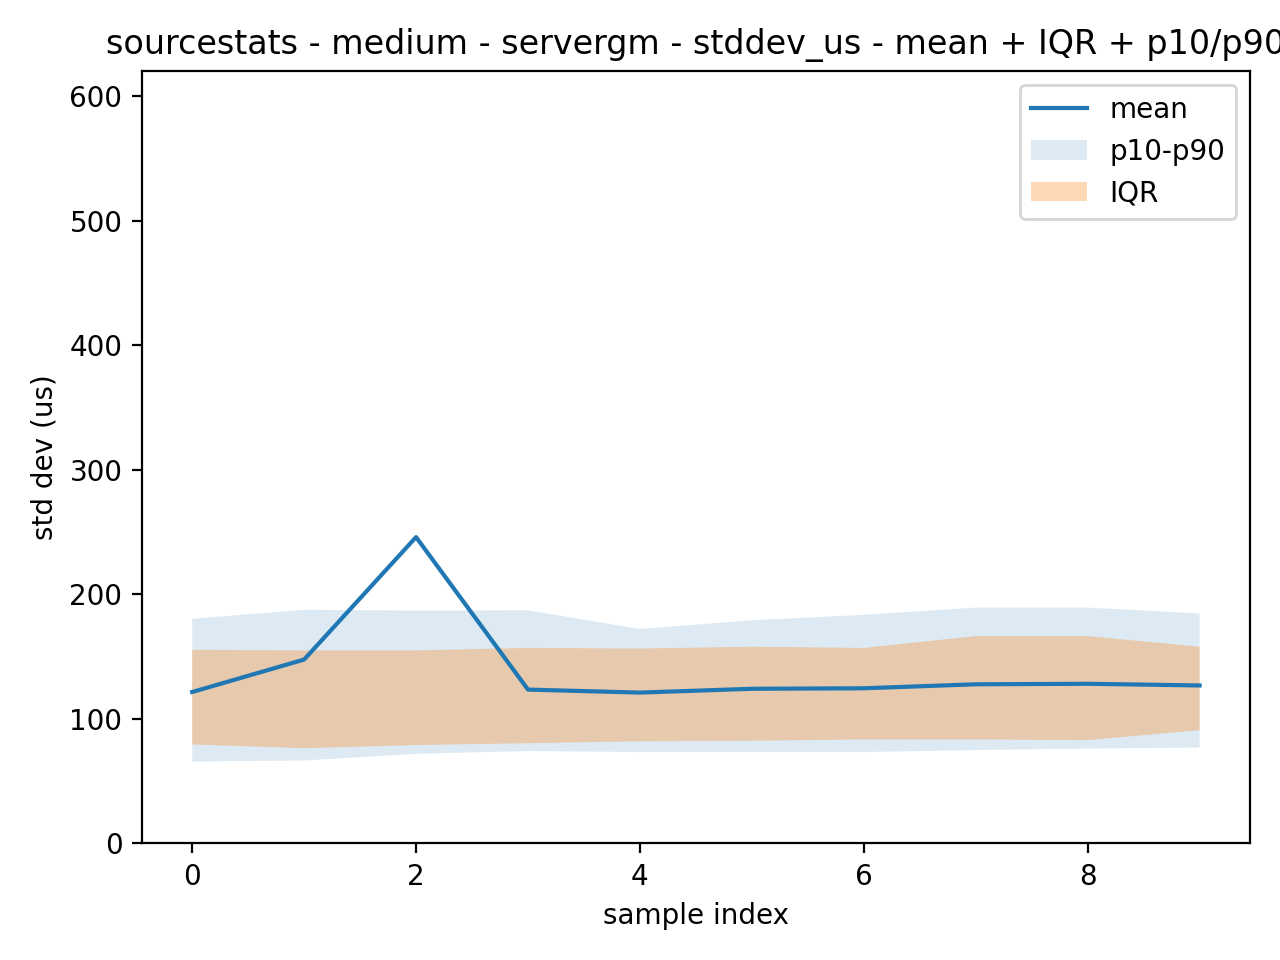
\includegraphics[width=\linewidth]{
      pars_plots/chrony_servergm/_aggregated/sourcestats/medium/servergm/stddev_us_mean_iqr_p10_p90.png
    }
    \caption{Scenario MEDIUM}
  \end{subfigure}
  \begin{subfigure}
    {0.32\textwidth}
    \centering
    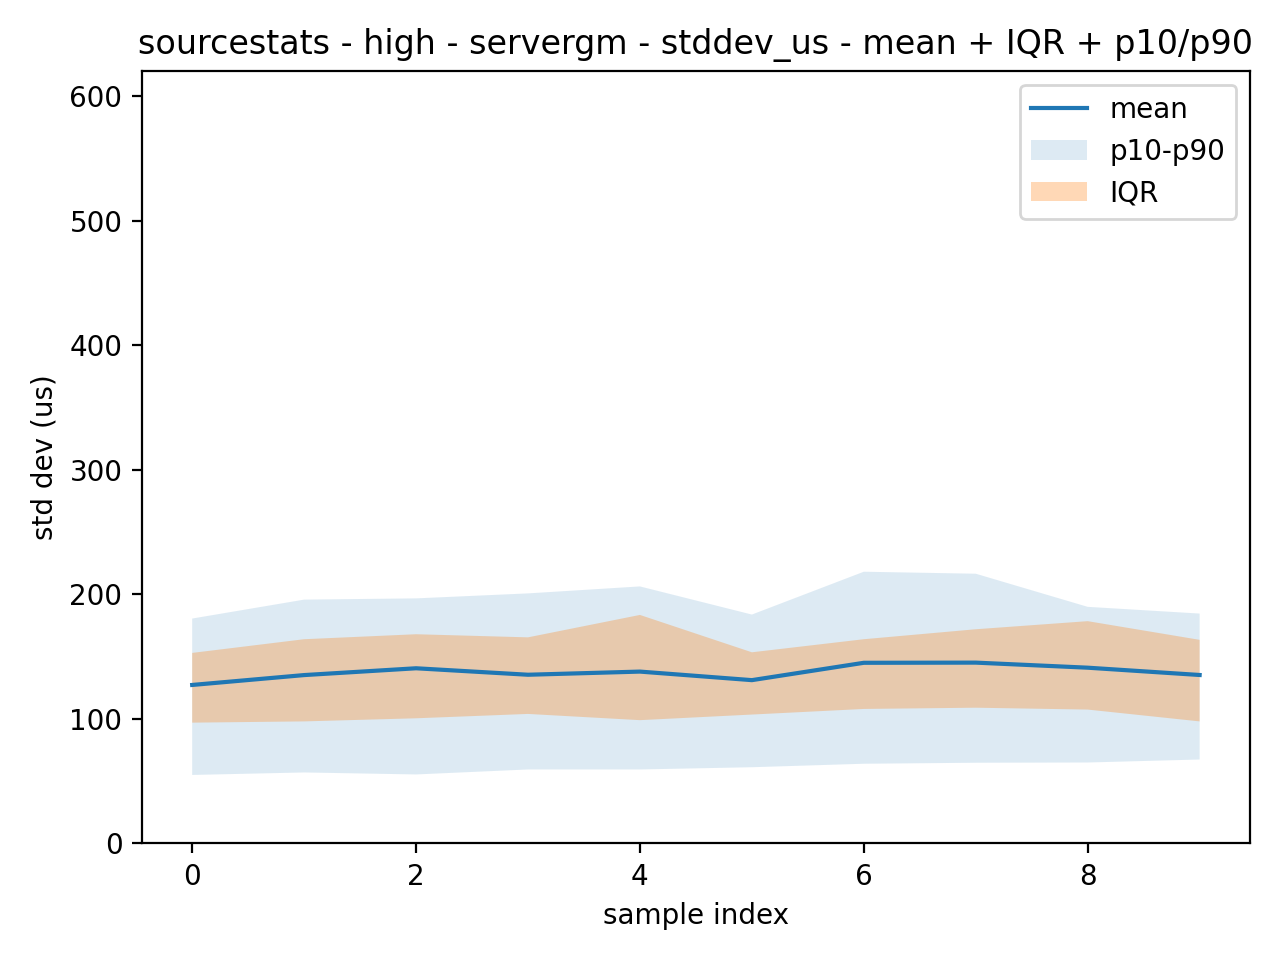
\includegraphics[width=\linewidth]{
      pars_plots/chrony_servergm/_aggregated/sourcestats/high/servergm/stddev_us_mean_iqr_p10_p90.png
    }
    \caption{Scenario HIGH}
  \end{subfigure}
  \caption{Media con banda interquartile e banda p10-p90 - nodo: \texttt{clientchrony}
  - netem/tc: \texttt{servergm}}
  \label{fig:scenario_comparison}
\end{figure}

\paragraph*{servergm - netem/tc:}
Nel caso della metrica \texttt{stddev\_us} riferita alla sezione \texttt{sourcestats},
l'analisi con impairment applicato sul nodo \texttt{servergm} evidenzia un comportamento
non monotono al variare dello scenario, ma con una chiara differenza tra il caso
\texttt{low}, più irregolare e disperso, e i casi \texttt{medium} e \texttt{high},
che risultano invece più compatti.

Nello scenario \texttt{low}, la curva delle medie si colloca sul livello più
elevato tra i tre scenari. La media aggregata risulta pari a \texttt{190.047 \,$\mu$s},
con una deviazione standard delle medie di \texttt{53.570 \,$\mu$s}; i valori medi
lungo la curva variano infatti tra \texttt{105.800 \,$\mu$s} e \texttt{268.400
\,$\mu$s}. Anche le bande di variabilità sono molto ampie: l'IQR medio è pari a \texttt{72.600
\,$\mu$s}, mentre l'ampiezza media dell'intervallo \texttt{p10-p90} raggiunge
\texttt{359.800 \,$\mu$s}, con picchi fino a \texttt{537.400 \,$\mu$s}. Le
statistiche globali sui campioni grezzi confermano questa forte dispersione, mostrando
una media complessiva di \texttt{190.047 \,$\mu$s}, una deviazione standard di \texttt{252.466
\,$\mu$s} e un valore massimo pari a \texttt{1622 \,$\mu$s}. Nel complesso, quindi,
lo scenario \texttt{low} descrive una stima della deviazione standard elevata e accompagnata
da una variabilità molto marcata tra le run, con presenza di outlier che
ampliano sensibilmente l'escursione osservata.

Nello scenario \texttt{medium}, il livello medio della metrica si riduce in
misura netta. La media aggregata della curva scende infatti a \texttt{139.160 \,$\mu$s},
con deviazione standard delle medie pari a \texttt{38.298 \,$\mu$s}. I valori medi
risultano compresi tra \texttt{121.133 \,$\mu$s} e \texttt{246.000 \,$\mu$s}.
Anche in questo caso le bande restano ampie, ma meno estese rispetto allo scenario
\texttt{low}: l'IQR medio vale \texttt{76.400 \,$\mu$s}, mentre l'intervallo medio
\texttt{p10-p90} è pari a \texttt{111.360 \,$\mu$s}. Le statistiche globali
confermano un ridimensionamento del livello medio, con media complessiva \texttt{139.160
\,$\mu$s} e mediana \texttt{130 \,$\mu$s}; tuttavia, resta una certa sensibilità a
valori estremi, come mostra il massimo pari a \texttt{2053 \,$\mu$s}. In termini
interpretativi, lo scenario \texttt{medium} mantiene una stima di variabilità
ancora significativa, ma più contenuta rispetto al caso \texttt{low}, e con un comportamento
della curva mediamente più raccolto.

Nello scenario \texttt{high}, la metrica si stabilizza ulteriormente attorno a un
livello medio simile, ma con una regolarità molto più marcata. La media aggregata
è pari a \texttt{137.440 \,$\mu$s}, dunque molto vicina al caso \texttt{medium}, ma
la deviazione standard delle medie scende drasticamente a \texttt{5.770 \,$\mu$s}.
Anche l'intervallo dei valori medi lungo la curva risulta molto ristretto,
compreso tra \texttt{127.267 \,$\mu$s} e \texttt{145.200 \,$\mu$s}. Le bande di dispersione
si contraggono: l'IQR medio è pari a \texttt{64.100 \,$\mu$s} e l'ampiezza media \texttt{p10-p90}
è \texttt{136.500 \,$\mu$s}, con oscillazioni grafiche molto più regolari lungo
i diversi indici campionari. Le statistiche globali sui dati grezzi confermano questa
lettura: la media complessiva è \texttt{137.440 \,$\mu$s}, la mediana è \texttt{141.500
\,$\mu$s} e il massimo osservato è \texttt{314 \,$\mu$s}, molto inferiore ai massimi
degli altri due scenari. Pertanto, nello scenario \texttt{high}, pur rimanendo la
metrica su un ordine di grandezza analogo a quello di \texttt{medium}, il comportamento
risulta sensibilmente più compatto e meno influenzato da run anomale.

Nel confronto complessivo emerge dunque una dinamica non lineare. Lo scenario
\texttt{low} è quello che presenta il livello medio più elevato e la maggiore dispersione,
sia nella curva aggregata sia nei campioni grezzi. Gli scenari \texttt{medium} e
\texttt{high} mostrano invece medie inferiori e molto simili tra loro, ma
differiscono sul piano della stabilità: \texttt{medium} conserva ancora una
dispersione non trascurabile, mentre \texttt{high} appare il caso più regolare e
compatto. Per la metrica \texttt{stddev\_us}, quindi, il degrado applicato sul
nodo \texttt{servergm} non determina un aumento progressivo della variabilità stimata
al crescere dello scenario; al contrario, il caso \texttt{low} risulta il più
penalizzante, mentre \texttt{high} mostra il comportamento complessivamente più
stabile.

\paragraph*{Confronto:}
Nel confronto tra i due casi emerge una differenza abbastanza netta. Con degrado
applicato su \texttt{servergm}, la metrica \texttt{stddev\_us} assume i valori medi
più elevati nello scenario \texttt{low} e poi si riduce nei casi \texttt{medium} e
\texttt{high}, con quest'ultimo che risulta il più stabile e compatto. Con
degrado applicato su \texttt{clientchrony}, invece, il massimo si osserva nello scenario
\texttt{medium}, mentre \texttt{high} riporta la metrica su livelli più bassi.

In termini comparativi, quindi, l'impairment sul server tende a produrre un
effetto più severo soprattutto nel caso \texttt{low}, accompagnato da una
dispersione molto marcata e da outlier più pronunciati. L'impairment sul client mostra
invece un comportamento più regolare, con variazioni meno estreme e una risposta
non monotona centrata sul caso \texttt{medium}. Nel complesso, il degrado lato \texttt{servergm}
appare quindi più sensibile alla presenza di condizioni instabili, mentre lato \texttt{clientchrony}
l'effetto resta più contenuto e distribuito in modo più omogeneo tra gli scenari.

\subsection{Analisi metrica: \texttt{system time offset}}
\begin{figure}[H]
  \centering

  \begin{subfigure}
    {0.32\textwidth}
    \centering
    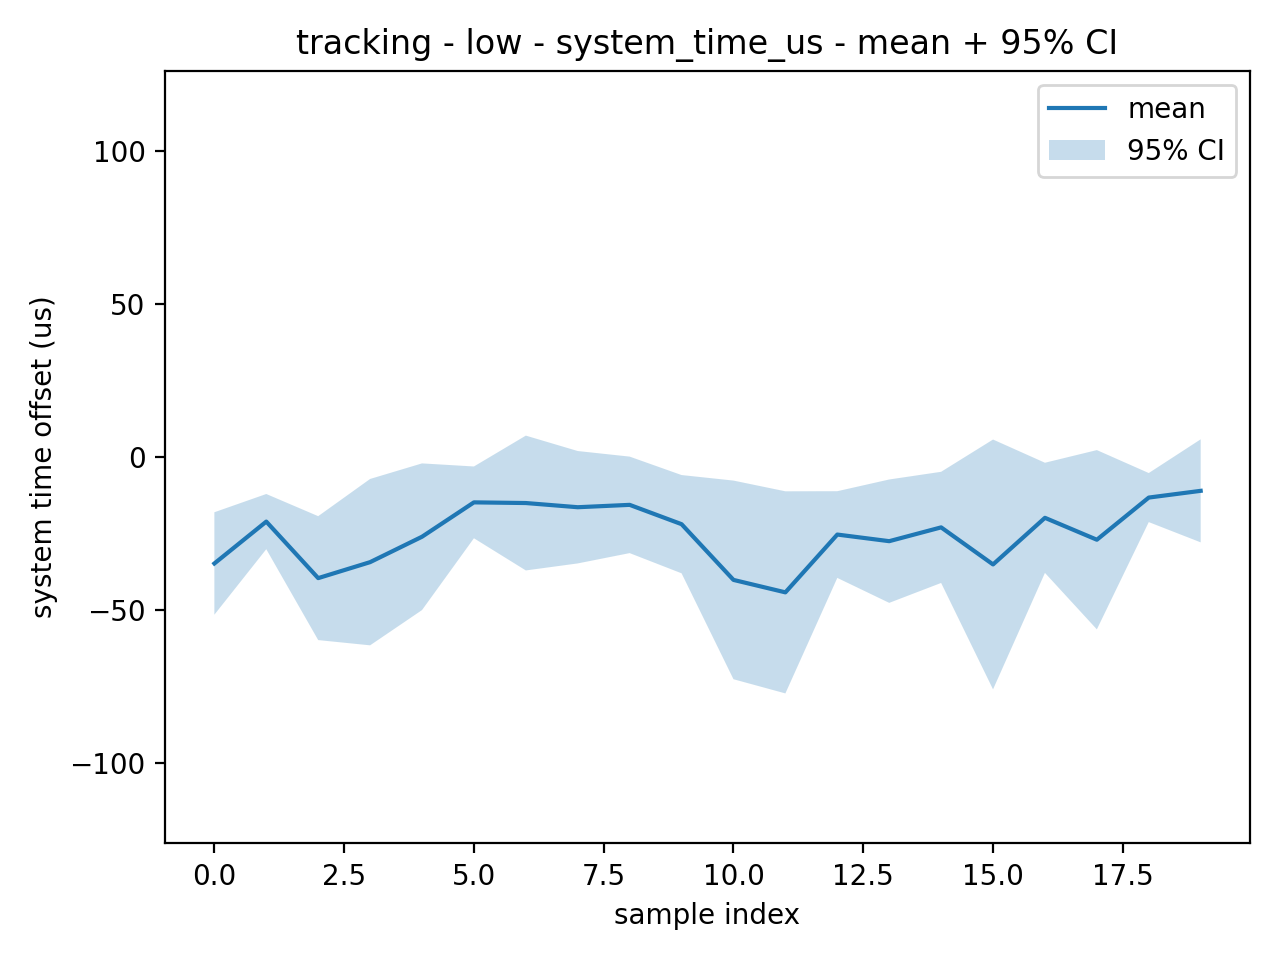
\includegraphics[width=\linewidth]{
      pars_plots/chrony_clientchrony/_aggregated/tracking/low/system_time_us_mean_ci95.png
    }
    \caption{Scenario LOW}
  \end{subfigure}
  \hfill
  \begin{subfigure}
    {0.32\textwidth}
    \centering
    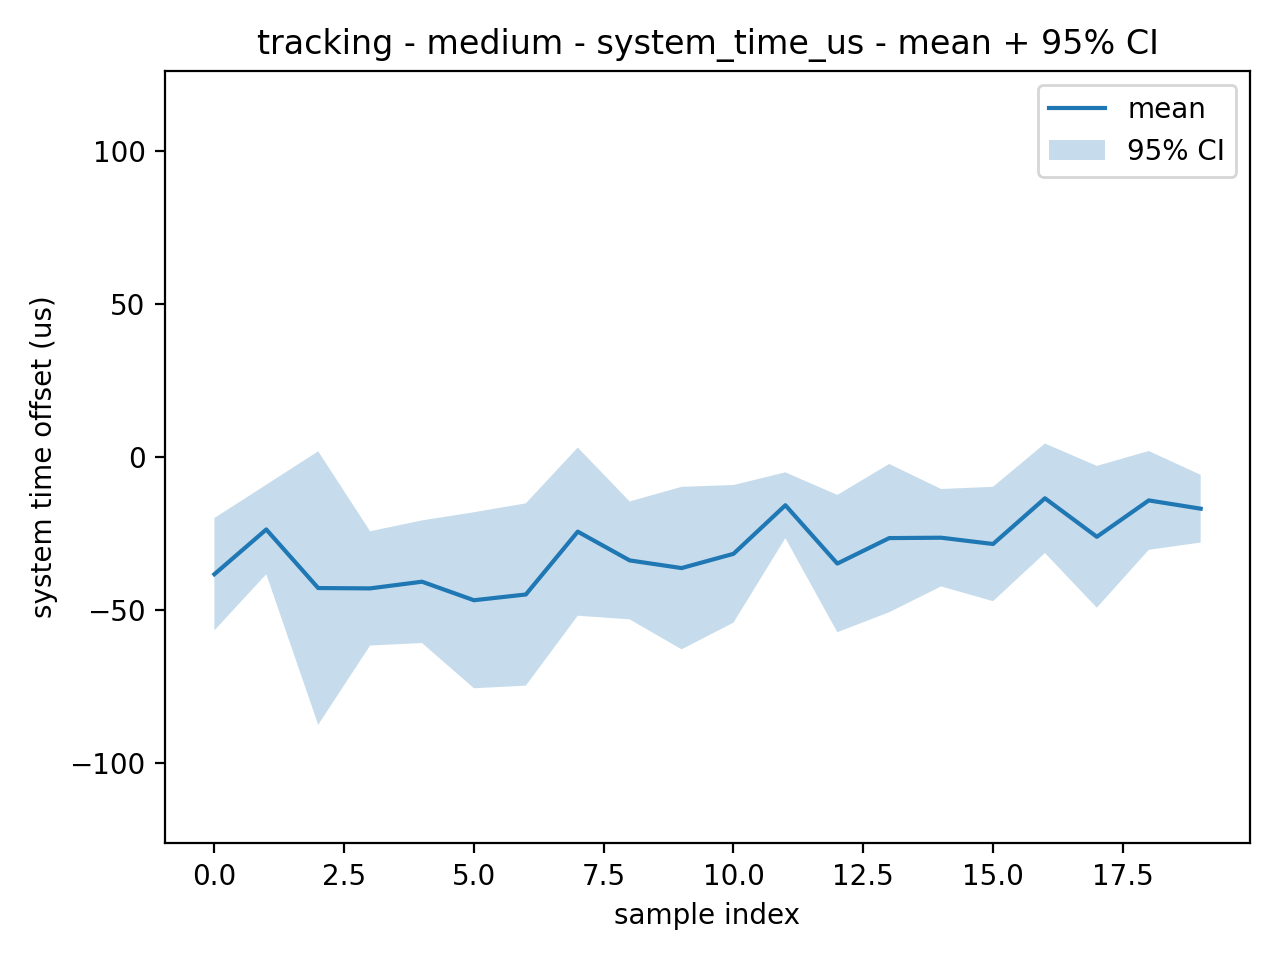
\includegraphics[width=\linewidth]{
      pars_plots/chrony_clientchrony/_aggregated/tracking/medium/system_time_us_mean_ci95.png
    }
    \caption{Scenario MEDIUM}
  \end{subfigure}
  \begin{subfigure}
    {0.32\textwidth}
    \centering
    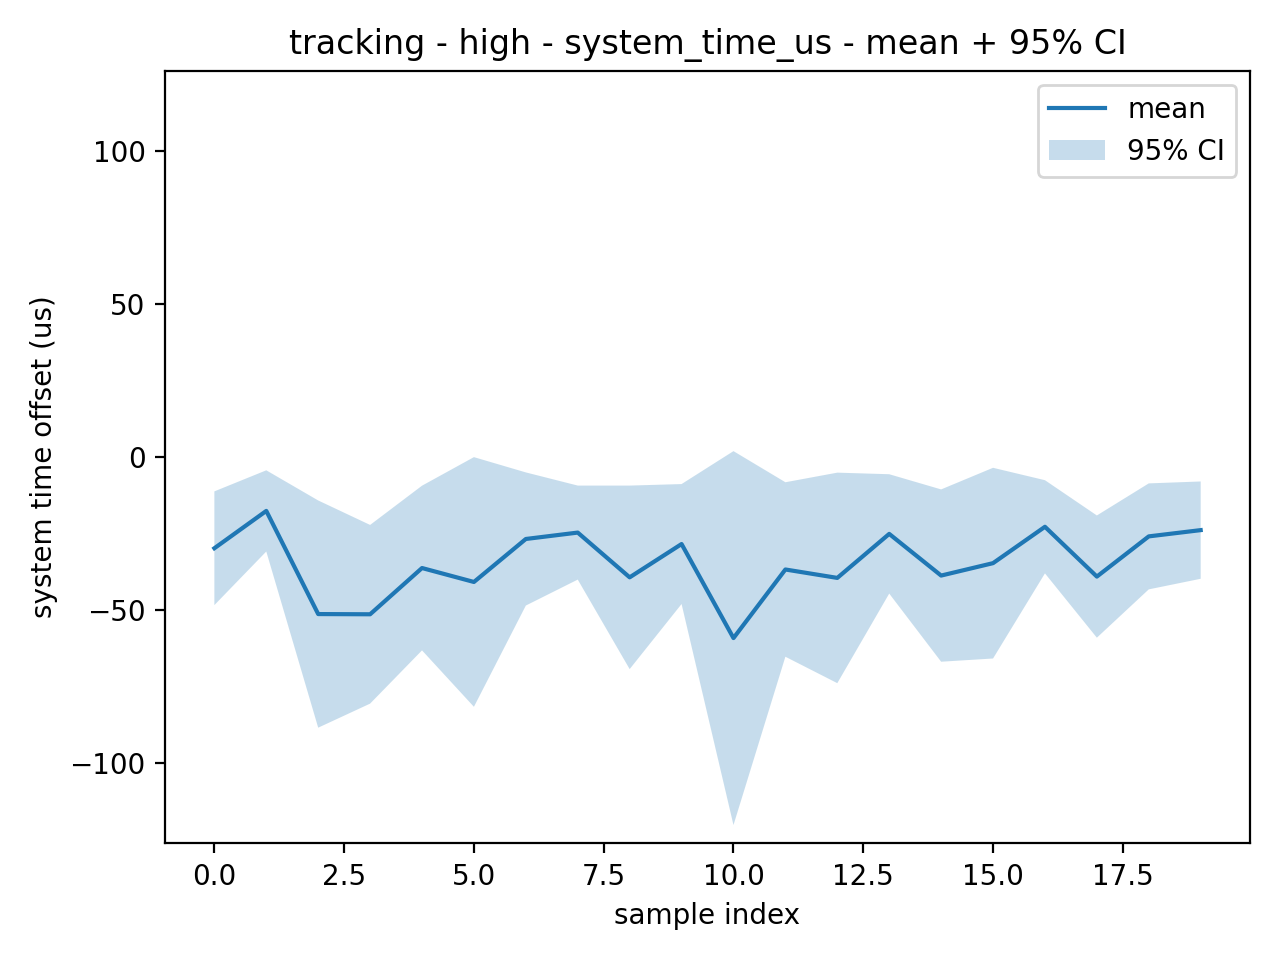
\includegraphics[width=\linewidth]{
      pars_plots/chrony_clientchrony/_aggregated/tracking/high/system_time_us_mean_ci95.png
    }
    \caption{Scenario HIGH}
  \end{subfigure}
  \caption{Media con intervallo di confidenza al 95\% - nodo: \texttt{clientchrony}
  - netem/tc: \texttt{clientchrony}}
  \label{fig:scenario_comparison}
\end{figure}
\begin{figure}[H]
  \centering

  \begin{subfigure}
    {0.32\textwidth}
    \centering
    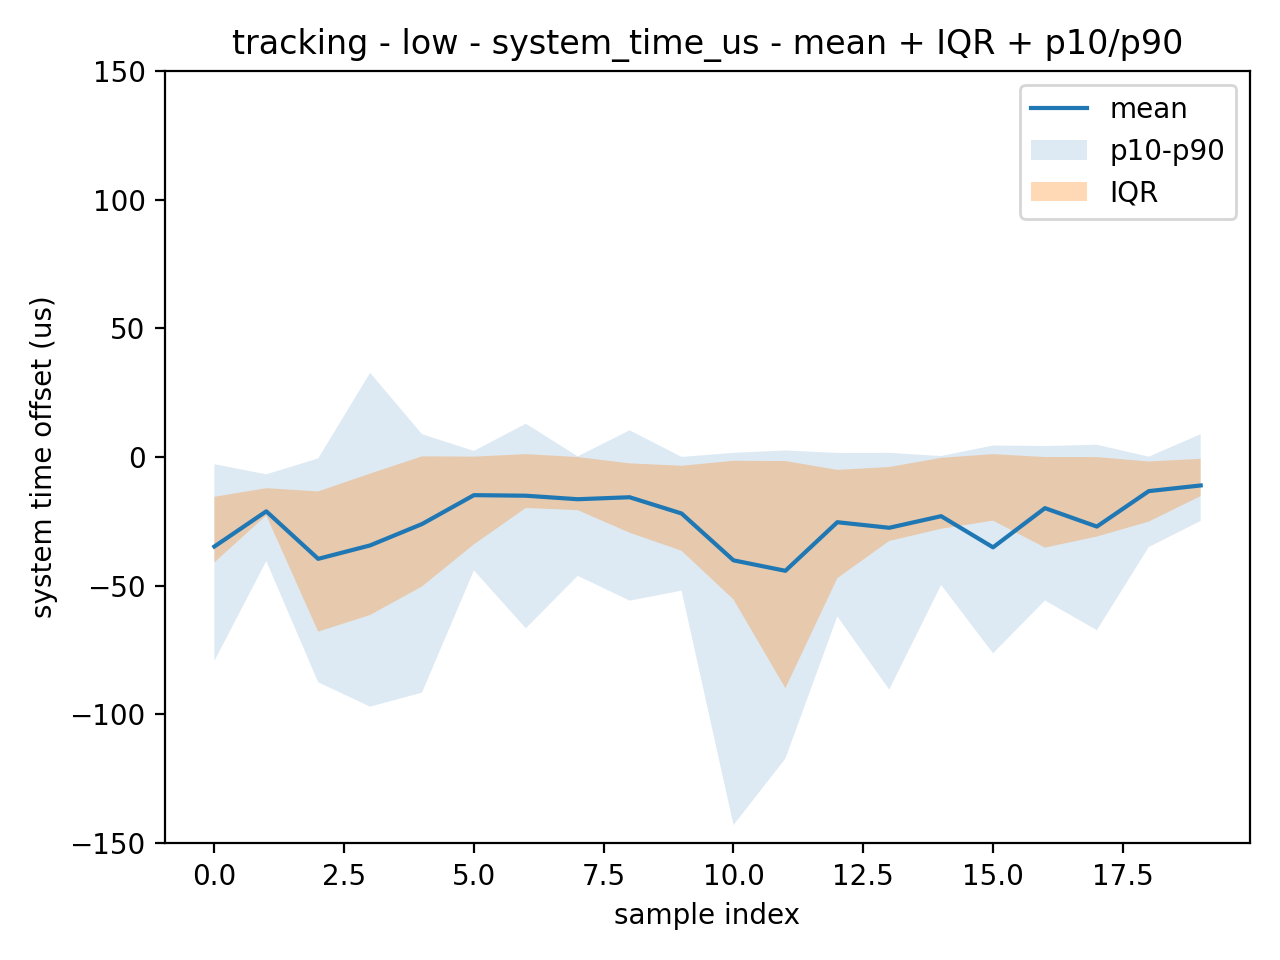
\includegraphics[width=\linewidth]{
      pars_plots/chrony_clientchrony/_aggregated/tracking/low/system_time_us_mean_iqr_p10_p90.png
    }
    \caption{Scenario LOW}
  \end{subfigure}
  \hfill
  \begin{subfigure}
    {0.32\textwidth}
    \centering
    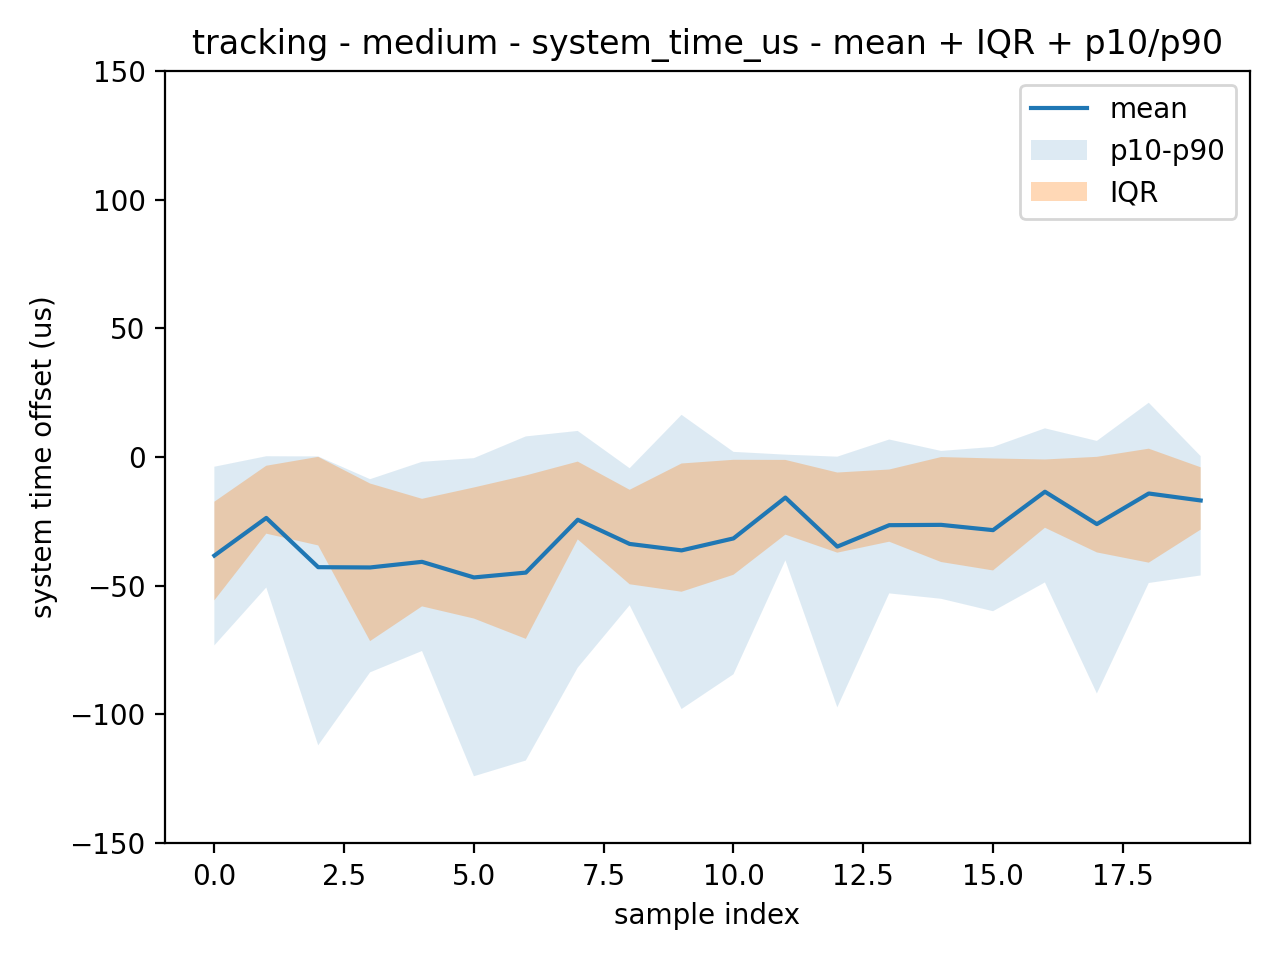
\includegraphics[width=\linewidth]{
      pars_plots/chrony_clientchrony/_aggregated/tracking/medium/system_time_us_mean_iqr_p10_p90.png
    }
    \caption{Scenario MEDIUM}
  \end{subfigure}
  \begin{subfigure}
    {0.32\textwidth}
    \centering
    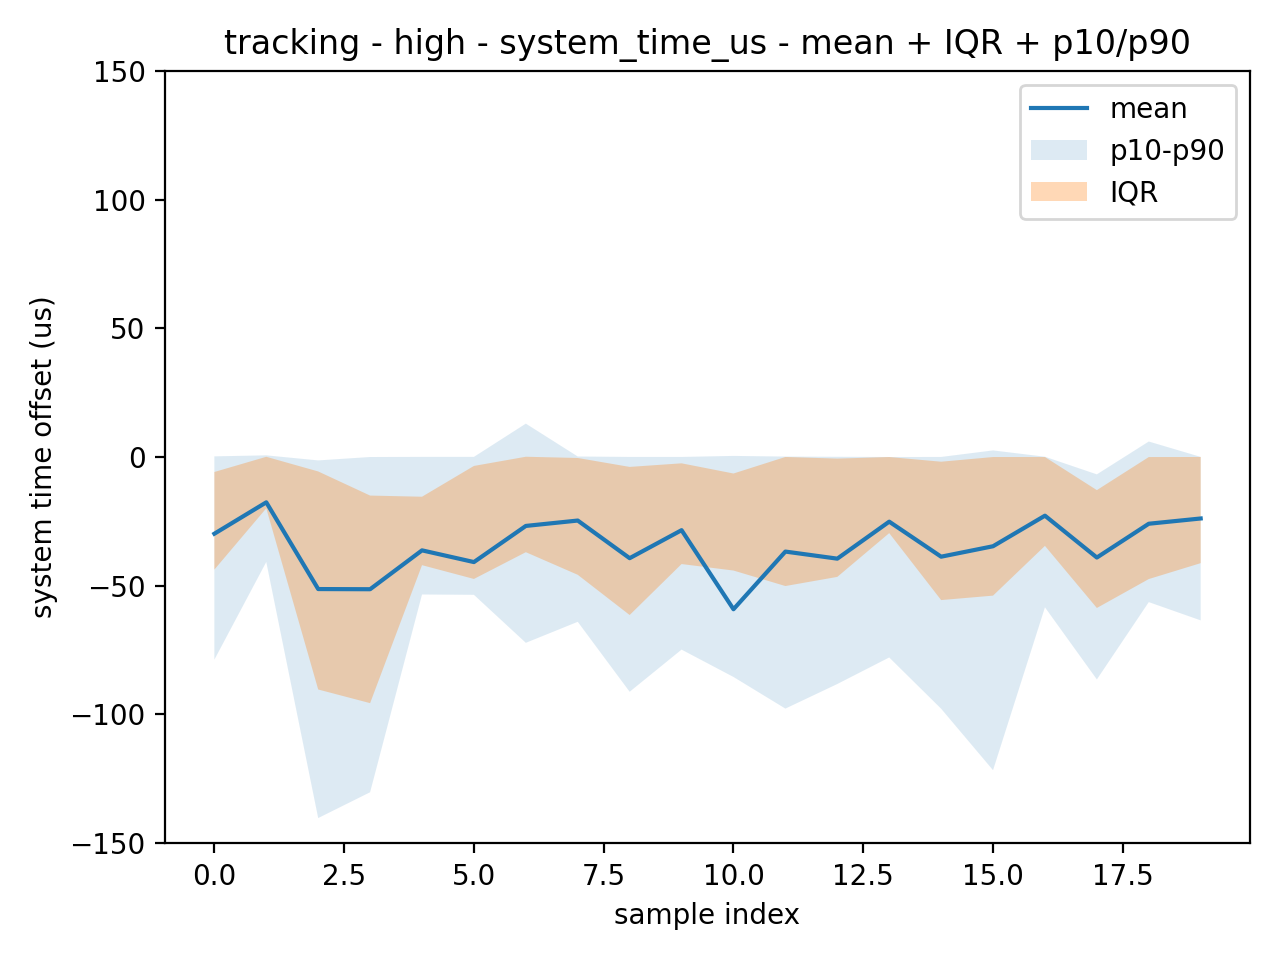
\includegraphics[width=\linewidth]{
      pars_plots/chrony_clientchrony/_aggregated/tracking/high/system_time_us_mean_iqr_p10_p90.png
    }
    \caption{Scenario HIGH}
  \end{subfigure}
  \caption{Media con banda interquartile e banda p10-p90 - nodo: \texttt{clientchrony}
  - netem/tc: \texttt{clientchrony}}
  \label{fig:scenario_comparison}
\end{figure}
\paragraph*{clientchrony - netem/tc:}
Nel caso della metrica \texttt{system\_time\_us}, l'analisi relativa a \texttt{clientchrony}
con degrado applicato sul nodo client evidenzia un comportamento più regolare
rispetto ad altre metriche, ma con una tendenza abbastanza chiara verso valori medi
progressivamente più negativi al crescere dell'intensità dello scenario. L'effetto
del degrado non si manifesta come instabilità esplosiva, bensì come uno spostamento
graduale del livello medio della curva, accompagnato da una variabilità che
rimane significativa ma nel complesso confrontabile nei tre casi.

Nello scenario \texttt{low}, la curva delle medie si mantiene costantemente su
valori negativi moderati. La media aggregata risulta pari a \texttt{-25.284 \,$\mu$s},
con deviazione standard delle medie \texttt{9.885 \,$\mu$s}; i valori della curva
risultano compresi tra \texttt{-44.187 \,$\mu$s} e \texttt{-11.031 \,$\mu$s}. I
grafici mostrano alcune oscillazioni locali, ma senza discontinuità marcate. Le
bande di dispersione restano ampie: l'IQR medio è pari a \texttt{35.089 \,$\mu$s},
mentre l'ampiezza media dell'intervallo \texttt{p10-p90} raggiunge \texttt{73.456
\,$\mu$s}, con picchi fino a \texttt{144.596 \,$\mu$s}. Anche i dati grezzi
confermano questo quadro, con media complessiva \texttt{-25.284 \,$\mu$s}, mediana
\texttt{-13.664 \,$\mu$s}, primo quartile \texttt{-34.557 \,$\mu$s} e terzo
quartile \texttt{-0.530 \,$\mu$s}. Nel complesso, quindi, lo scenario \texttt{low}
descrive un offset del tempo di sistema stabilmente negativo, ma ancora
contenuto entro poche decine di microsecondi nella maggior parte dei campioni.

Nello scenario \texttt{medium}, il livello medio si sposta ulteriormente verso
valori più negativi. La media aggregata della curva scende infatti a \texttt{-30.408
\,$\mu$s}, con deviazione standard delle medie pari a \texttt{10.531 \,$\mu$s}; i
valori medi lungo la curva variano tra \texttt{-46.762 \,$\mu$s} e \texttt{-13.465
\,$\mu$s}. L'andamento rimane abbastanza regolare e non mostra rotture
improvvise, ma si colloca complessivamente su un livello più basso rispetto al caso
\texttt{low}. Anche le bande di dispersione restano ampie, sebbene leggermente
più raccolte nella parte centrale: l'IQR medio vale \texttt{39.129 \,$\mu$s}, mentre
l'intervallo medio \texttt{p10-p90} è \texttt{78.520 \,$\mu$s}. Le statistiche
globali sui campioni grezzi confermano questo lieve peggioramento, con media complessiva
\texttt{-30.408 \,$\mu$s}, mediana \texttt{-22.285 \,$\mu$s} e quartili pari a
\texttt{-46.666 \,$\mu$s} e \texttt{-2.351 \,$\mu$s}. In termini interpretativi,
lo scenario \texttt{medium} non altera drasticamente la forma del fenomeno, ma
rende più marcato il bias negativo del tempo di sistema rispetto alla sorgente.

Nello scenario \texttt{high}, la tendenza osservata nei casi precedenti si
accentua ulteriormente. La media aggregata della curva raggiunge \texttt{-34.573 \,$\mu$s},
il valore più negativo tra i tre scenari, mentre la deviazione standard delle
medie è \texttt{10.809 \,$\mu$s}. I valori medi lungo la curva oscillano tra
\texttt{-59.120 \,$\mu$s} e \texttt{-17.588 \,$\mu$s}, mantenendosi quindi stabilmente
più bassi rispetto agli altri due casi. Anche le bande di dispersione risultano
comparabili o leggermente più ampie: l'IQR medio è \texttt{45.637 \,$\mu$s} e l'ampiezza
media \texttt{p10-p90} è \texttt{82.403 \,$\mu$s}. I dati grezzi confermano il medesimo
assetto, con media complessiva \texttt{-34.573 \,$\mu$s}, mediana \texttt{-19.111
\,$\mu$s}, primo quartile \texttt{-48.642 \,$\mu$s} e terzo quartile prossimo allo
zero, pari a \texttt{0.001 \,$\mu$s}. Anche in questo scenario, dunque, il
sistema resta operativo, ma il tempo di sistema si colloca mediamente su valori più
negativi e con una dispersione ancora significativa.

Nel confronto complessivo tra i tre scenari emerge quindi una dinamica più lineare
rispetto a quanto osservato per altre metriche. Il passaggio da \texttt{low} a \texttt{medium}
e poi a \texttt{high} produce infatti un progressivo spostamento del livello medio
verso valori più negativi: \texttt{-25.284 \,$\mu$s}, \texttt{-30.408 \,$\mu$s} e
\texttt{-34.573 \,$\mu$s}. La variabilità rimane ampia in tutti e tre i casi e non
cresce in modo altrettanto netto, ma il bias medio negativo del \texttt{system\_time\_us}
diventa gradualmente più pronunciato all'aumentare del degrado. Pertanto, per questa
metrica, l'effetto del netem applicato su \texttt{clientchrony} appare soprattutto
come una deriva progressiva del livello centrale della misura, piuttosto che
come un aumento drastico dell'instabilità.

\begin{figure}[H]
  \centering

  \begin{subfigure}
    {0.32\textwidth}
    \centering
    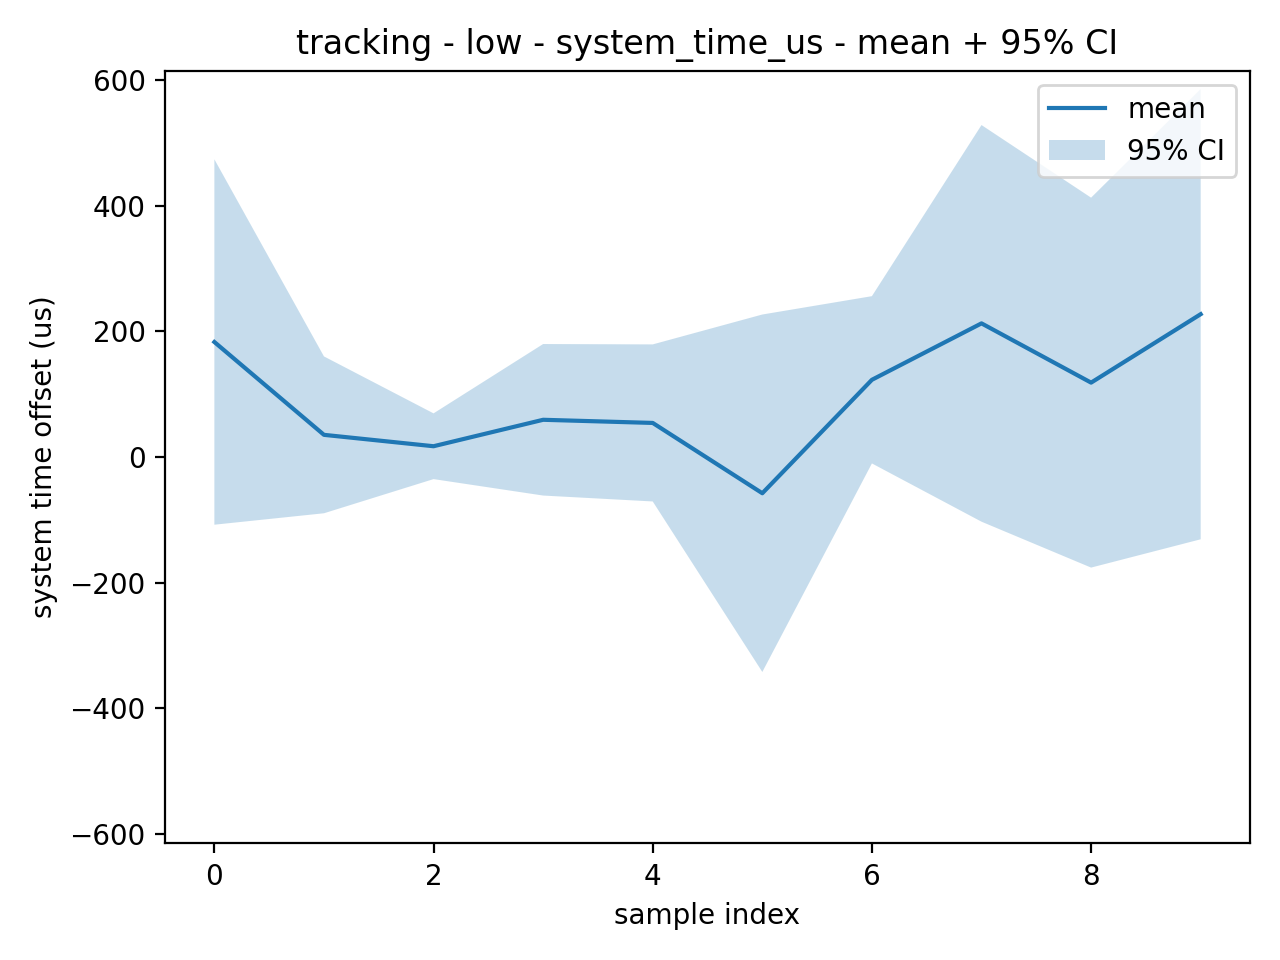
\includegraphics[width=\linewidth]{
      pars_plots/chrony_servergm/_aggregated/tracking/low/system_time_us_mean_ci95.png
    }
    \caption{Scenario LOW}
  \end{subfigure}
  \hfill
  \begin{subfigure}
    {0.32\textwidth}
    \centering
    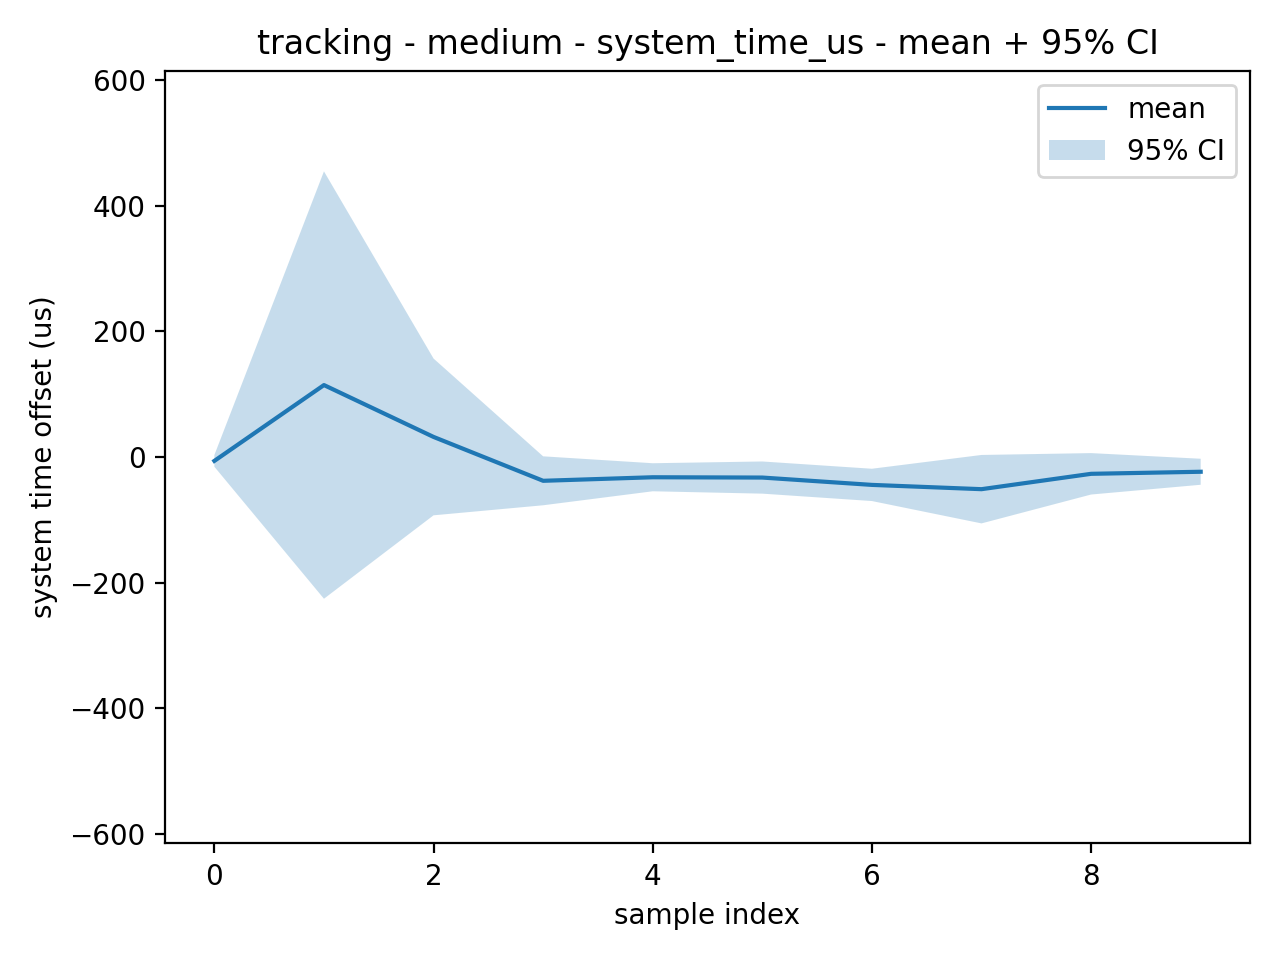
\includegraphics[width=\linewidth]{
      pars_plots/chrony_servergm/_aggregated/tracking/medium/system_time_us_mean_ci95.png
    }
    \caption{Scenario MEDIUM}
  \end{subfigure}
  \begin{subfigure}
    {0.32\textwidth}
    \centering
    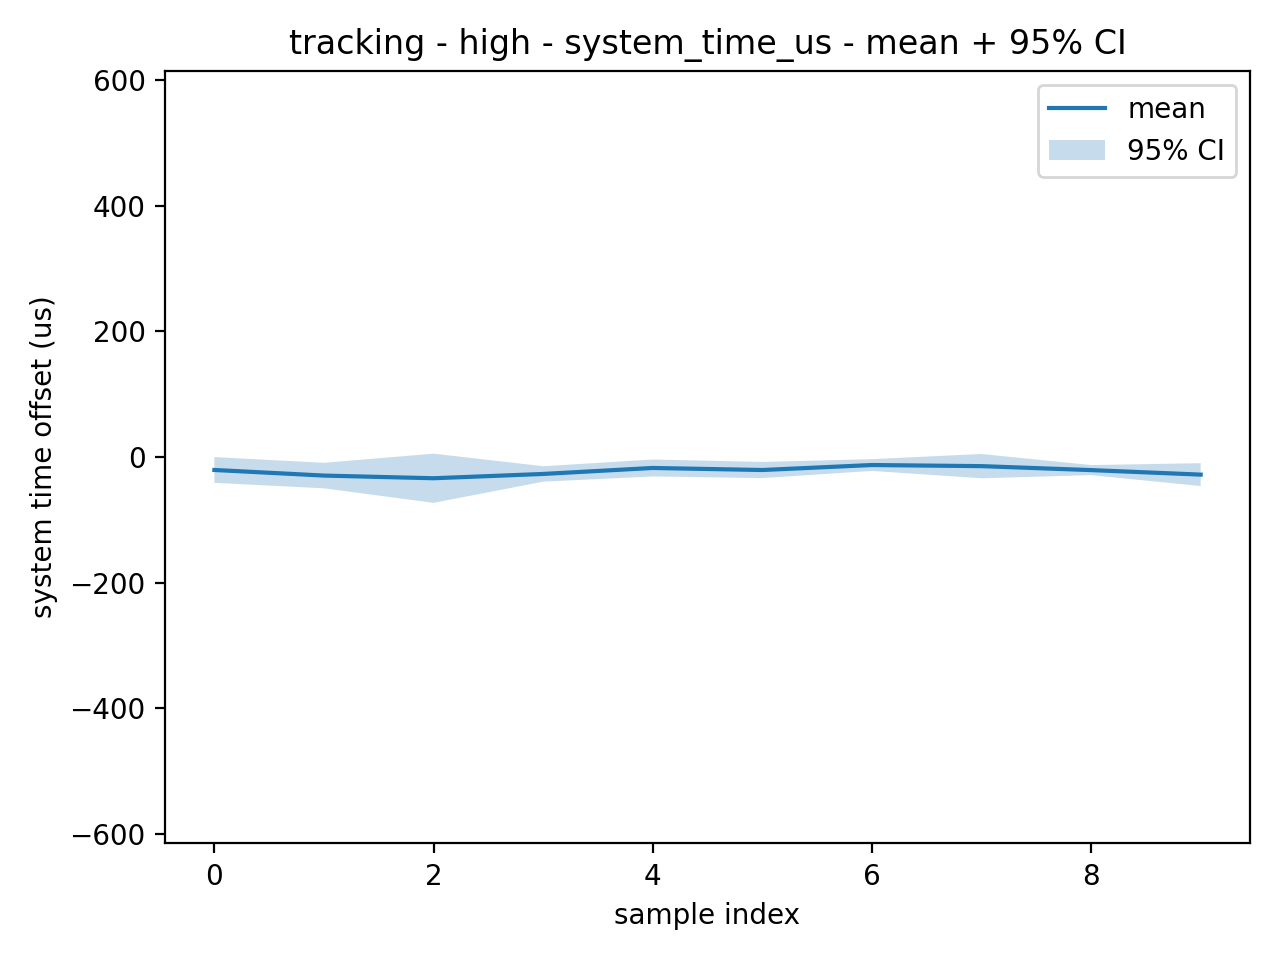
\includegraphics[width=\linewidth]{
      pars_plots/chrony_servergm/_aggregated/tracking/high/system_time_us_mean_ci95.png
    }
    \caption{Scenario HIGH}
  \end{subfigure}
  \caption{Media con intervallo di confidenza al 95\% - nodo: \texttt{clientchrony}
  - netem/tc: \texttt{servergm}}
  \label{fig:scenario_comparison}
\end{figure}
\begin{figure}[H]
  \centering

  \begin{subfigure}
    {0.32\textwidth}
    \centering
    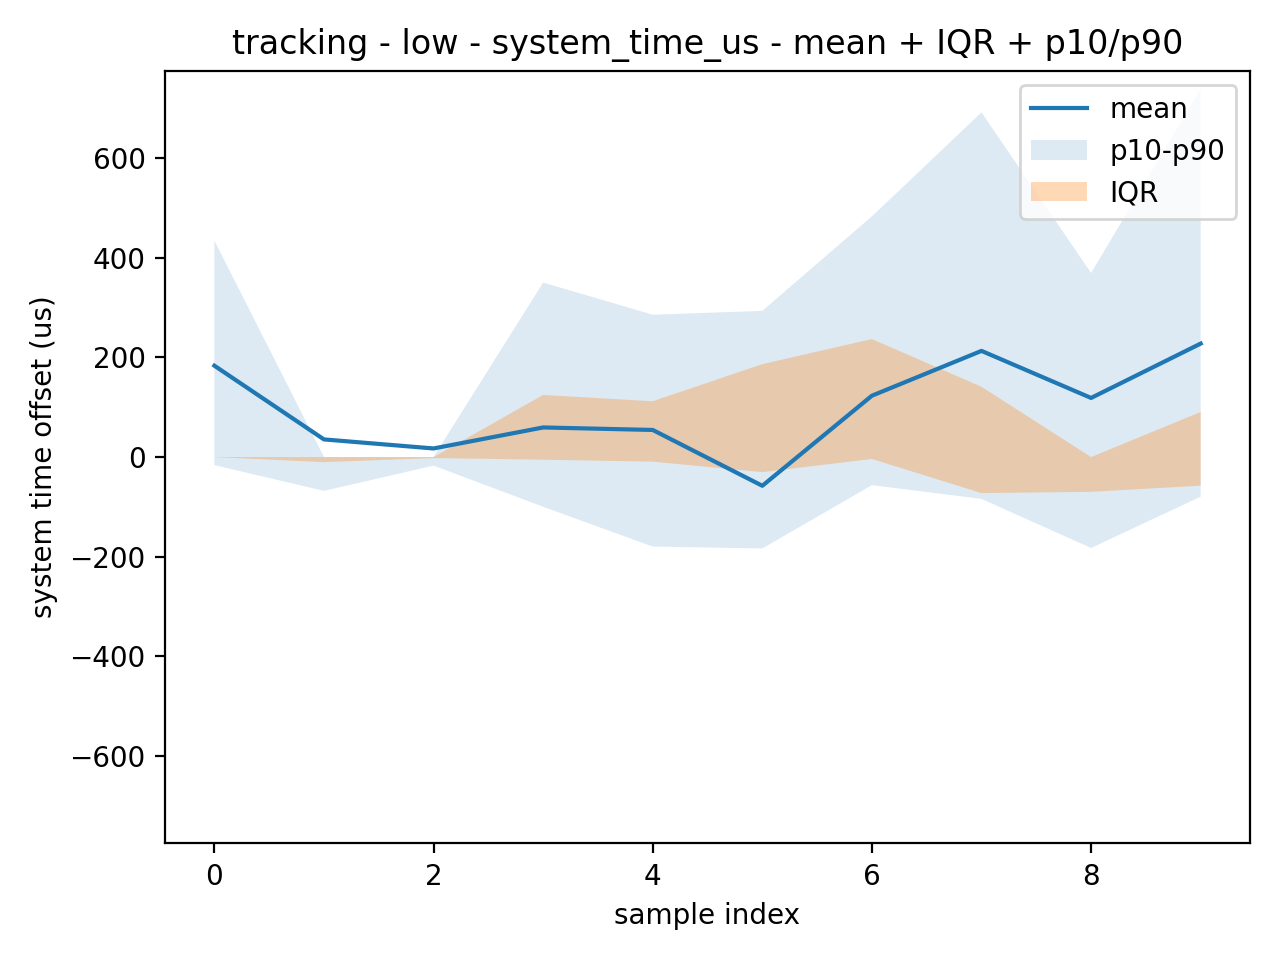
\includegraphics[width=\linewidth]{
      pars_plots/chrony_servergm/_aggregated/tracking/low/system_time_us_mean_iqr_p10_p90.png
    }
    \caption{Scenario LOW}
  \end{subfigure}
  \hfill
  \begin{subfigure}
    {0.32\textwidth}
    \centering
    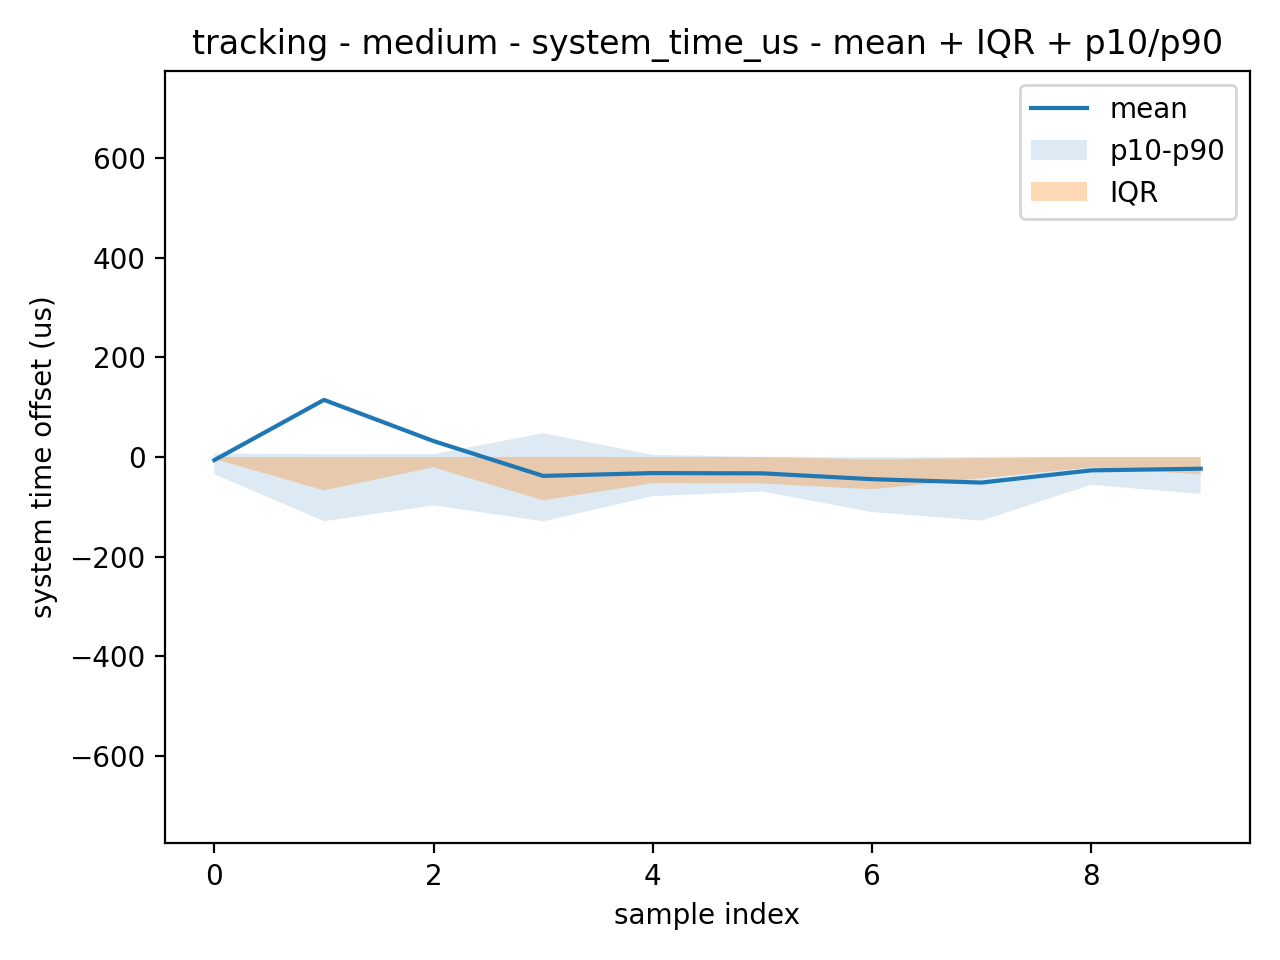
\includegraphics[width=\linewidth]{
      pars_plots/chrony_servergm/_aggregated/tracking/medium/system_time_us_mean_iqr_p10_p90.png
    }
    \caption{Scenario MEDIUM}
  \end{subfigure}
  \begin{subfigure}
    {0.32\textwidth}
    \centering
    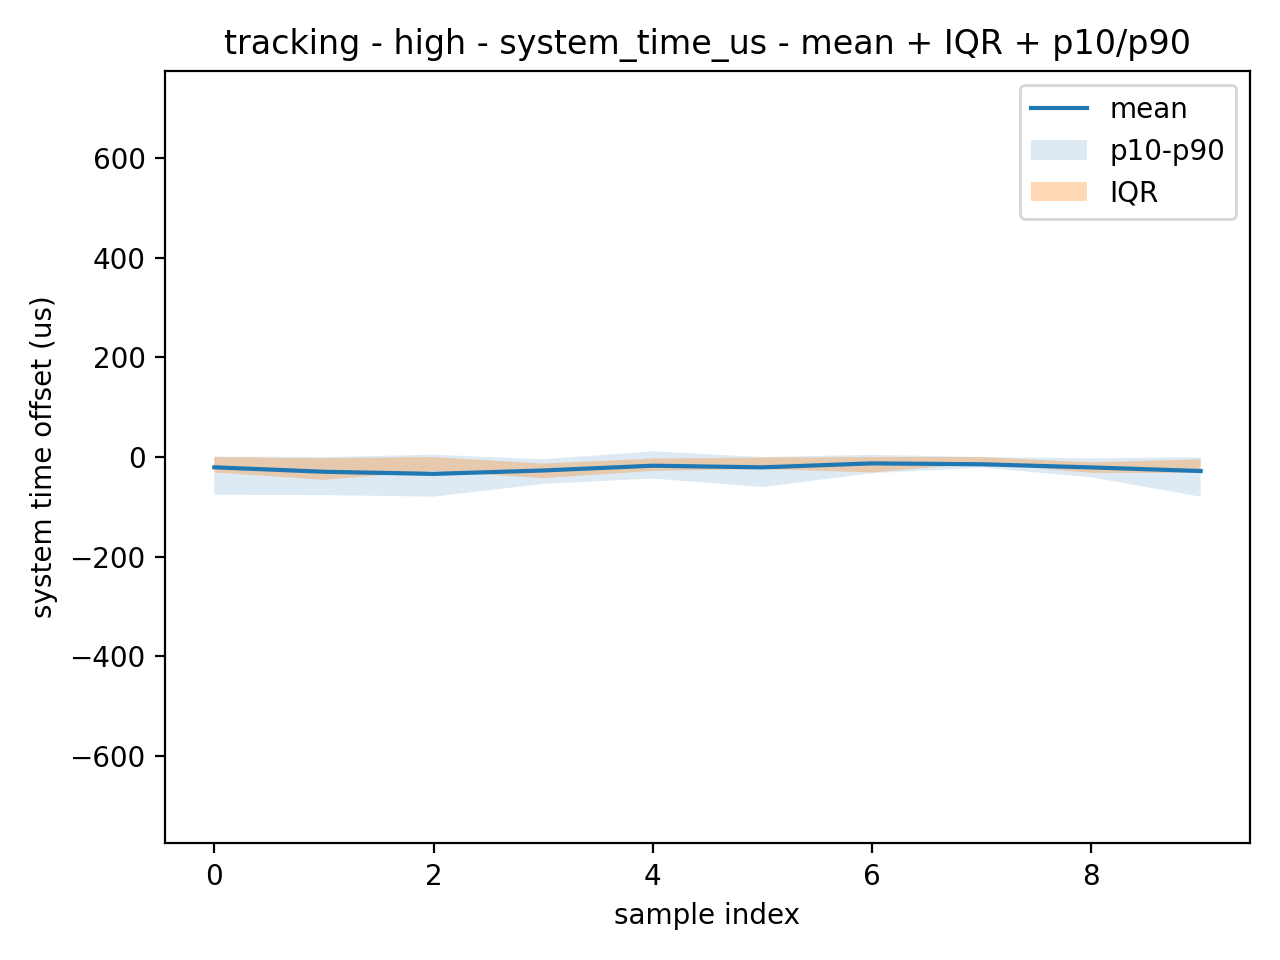
\includegraphics[width=\linewidth]{
      pars_plots/chrony_servergm/_aggregated/tracking/high/system_time_us_mean_iqr_p10_p90.png
    }
    \caption{Scenario HIGH}
  \end{subfigure}
  \caption{Media con banda interquartile e banda p10-p90 - nodo: \texttt{clientchrony}
  - netem/tc: \texttt{servergm}}
  \label{fig:scenario_comparison}
\end{figure}

\paragraph*{servergm - netem/tc:}
Nel caso della metrica \texttt{system\_time\_us} riferita alla sezione \texttt{tracking},
l'analisi con impairment applicato sul nodo \texttt{servergm} evidenzia un
comportamento fortemente non monotono al variare dello scenario. Il caso \texttt{low}
risulta nettamente il più irregolare e disperso, mentre gli scenari \texttt{medium}
e soprattutto \texttt{high} mostrano una sensibile contrazione sia del livello medio
sia della variabilità, pur mantenendo un offset del tempo di sistema
prevalentemente negativo.

Nello scenario \texttt{low}, la metrica assume il livello medio più elevato tra
i tre casi ed è accompagnata dalla maggiore dispersione osservata nell'intera
analisi. La media aggregata della curva è pari a \texttt{97.407 \,$\mu$s}, con deviazione
standard delle medie pari a \texttt{92.121 \,$\mu$s}; i valori medi lungo la curva
risultano compresi tra \texttt{-57.631 \,$\mu$s} e \texttt{227.575 \,$\mu$s}. I
grafici mostrano infatti una curva molto irregolare, con alternanza tra valori moderatamente
positivi e una flessione negativa locale, oltre a bande di incertezza molto
ampie. Tale quadro è confermato dagli indicatori di dispersione: l'IQR medio è
\texttt{115.127 \,$\mu$s}, mentre l'ampiezza media dell'intervallo \texttt{p10-p90}
raggiunge \texttt{461.010 \,$\mu$s}, con picchi fino a \texttt{817.440 \,$\mu$s}.
Anche i dati grezzi confermano un comportamento estremamente disperso, con media
complessiva \texttt{97.407 \,$\mu$s}, deviazione standard \texttt{418.691 \,$\mu$s}
e un valore massimo pari a \texttt{2342.321 \,$\mu$s}. In termini interpretativi,
lo scenario \texttt{low} descrive quindi una risposta molto instabile, con forte
eterogeneità tra run e presenza di episodi anomali che trascinano la media su
valori positivi elevati.

Nello scenario \texttt{medium}, il comportamento cambia in modo netto. La media aggregata
della curva scende a \texttt{-10.765 \,$\mu$s}, passando dunque da un livello chiaramente
positivo a uno leggermente negativo. La deviazione standard delle medie si
riduce a \texttt{49.927 \,$\mu$s}, circa la metà del valore osservato nel caso
\texttt{low}, mentre i valori della curva si collocano tra \texttt{-51.169 \,$\mu$s}
e \texttt{114.676 \,$\mu$s}. Anche visivamente il grafico mostra un picco iniziale
positivo più pronunciato, seguito però da una stabilizzazione su valori
moderatamente negativi. Le bande di dispersione si restringono sensibilmente rispetto
al caso precedente: l'IQR medio è pari a \texttt{43.947 \,$\mu$s} e l'intervallo medio
\texttt{p10-p90} vale \texttt{97.563 \,$\mu$s}. I dati grezzi confermano il
ridimensionamento del fenomeno, con media complessiva \texttt{-10.765 \,$\mu$s}, mediana
\texttt{-7.355 \,$\mu$s} e quartili pari a \texttt{-50.338 \,$\mu$s} e \texttt{0.031
\,$\mu$s}. Pertanto, nello scenario \texttt{medium}, il tempo di sistema resta
variabile ma risulta nel complesso molto meno disperso del caso \texttt{low},
con una tendenza centrale tornata leggermente sotto lo zero.

Nello scenario \texttt{high}, la metrica mostra il comportamento più compatto e
regolare. La media aggregata della curva è pari a \texttt{-22.466 \,$\mu$s}, quindi
più negativa rispetto al caso \texttt{medium}, ma accompagnata da una deviazione standard
delle medie molto contenuta, pari a soli \texttt{6.852 \,$\mu$s}. L'intervallo
dei valori medi lungo la curva è infatti ristretto, compreso tra \texttt{-33.763 \,$\mu$s}
e \texttt{-12.696 \,$\mu$s}, e il grafico mostra una linea quasi piatta attorno
a valori debolmente negativi. Anche gli indicatori di dispersione confermano questo
assetto più stabile: l'IQR medio è \texttt{27.040 \,$\mu$s}, mentre l'ampiezza
media \texttt{p10-p90} è \texttt{57.641 \,$\mu$s}, entrambe inferiori ai valori osservati
negli altri due scenari. Le statistiche globali sui campioni grezzi sono
coerenti con tale lettura, con media complessiva \texttt{-22.466 \,$\mu$s}, deviazione
standard \texttt{34.432 \,$\mu$s} e massimo pari a \texttt{39.212 \,$\mu$s},
molto inferiore ai picchi degli altri scenari. In questo caso, dunque, il degrado
non si traduce in una maggiore instabilità, ma in un comportamento più raccolto
attorno a un offset negativo moderato.

Nel confronto complessivo tra i tre scenari emerge quindi una dinamica
fortemente non lineare. Lo scenario \texttt{low} è nettamente il più disperso e
presenta anche il livello medio più elevato, positivo e influenzato da run molto anomale.
Lo scenario \texttt{medium} riduce drasticamente tale effetto, riportando la
metrica su valori medi prossimi ma inferiori allo zero e contraendo in misura
sostanziale la variabilità. Lo scenario \texttt{high} accentua ulteriormente
questa stabilizzazione, risultando il caso più compatto e regolare, pur con una
media leggermente più negativa. Per la metrica \texttt{system\_time\_us}, quindi,
il degrado applicato sul nodo \texttt{servergm} non produce un peggioramento progressivo
all'aumentare dello scenario, ma una risposta sperimentale in cui il caso
\texttt{low} rappresenta la condizione più critica, mentre \texttt{medium} e soprattutto
\texttt{high} mostrano un comportamento via via più stabile.

\paragraph*{Confronto:}
Nel confronto tra i due punti di applicazione del degrado non emerge una superiorità
univoca di uno scenario rispetto all'altro. Con impairment applicato su \texttt{clientchrony},
la metrica \texttt{system\_time\_us} mostra un andamento più regolare e soprattutto
un peggioramento progressivo al crescere dell'intensità dello scenario,
evidenziando quindi una risposta più monotona al degrado. Con impairment applicato
su \texttt{servergm}, invece, il comportamento è meno lineare: non si osserva una
crescita progressiva del deterioramento, ma compare una condizione fortemente
anomala nello scenario \texttt{low}, caratterizzata da dispersione molto elevata
e valori medi sensibilmente più instabili.